\documentclass[letterpaper,10pt]{book}
% Change to 10 pt
\usepackage{pdfpages}
\usepackage{morewrites}			% to counteract the no write space problem
\setcounter{tocdepth}{6}

\usepackage[framemethod=TikZ]{mdframed}

\usepackage{fancyhdr}

\usepackage{paralist}
\usepackage{amsmath}
\usepackage{amsfonts}
\usepackage{amssymb}
\usepackage{graphicx}

\usepackage{datetime}
%\usepackage{ulem}

%\usepackage[nottoc]{toobibind}

\usepackage[inline]{enumitem}

% Outer margin at 2.50 is exacty correct to fit the ``corruption alert'' tables
\usepackage[inner=1.0in, outer=2.50in, top=2.54cm,bottom=2.54cm, marginparwidth=2.25in]{geometry}

\usepackage{marginnote}
\usepackage{longtable}
\usepackage{booktabs}
\usepackage{xcolor}

\usepackage{soul}

%%%%%%%%%%%%
\definecolor{ForestGreen}{rgb}{0.00,0.29,0.098}
%%%%%%%%%%%%

\usepackage{marginnote}

\usepackage{imakeidx} 
\usepackage[
	backref=true,
	style=numeric,
%	citestyle=numeric,
	backend=bibtex
	]{biblatex}
\usepackage[driverfallback=hypertex,colorlinks=True]{hyperref}
\usepackage{cleveref}

\makeindex[name=scripture,columnsep=20pt, columnseprule=True,columns=3, title=Scripture References]
\makeindex[name=speaker,columnsep=20pt, columnseprule=True,,columns=2, title=Sermon Creator]
\makeindex[name=series,columnsep=20pt, columnseprule=True,,columns=2, title=Sermon Series]
\makeindex[name=date,columnsep=20pt, columnseprule=True,columns=2, title=Sermon Date]

\makeindex[name=event,columnsep=20pt, columnseprule=True,columns=2, title=Event]

\makeindex[name=topic,columnsep=20pt, columnseprule=True,columns=2, title=Topic]
\makeindex[name=AWIP,columnsep=20pt, columnseprule=True,columns=3, title=All Words in Passage]
\makeindex[name=NWIV,columnsep=20pt, columnseprule=True,columns=3, title=Number of Words in Verse]
\makeindex[name=PNIP,columnsep=20pt, columnseprule=True,columns=3, title=Proper Names in Passage]
\makeindex[name=PEIP,columnsep=20pt, columnseprule=True,columns=2, title=Prophetic Events in Passage]

\makeindex[name=TWPAQ,columnsep=20pt, columnseprule=True,columns=1, title=13-Word Phrases and Quotes]
\makeindex[name=PFTTIS,columnsep=20pt, columnseprule=False,columns=3, title=Phrases found 13 times in scripture]
\makeindex[name=WFTTIS,columnsep=20pt, columnseprule=False,columns=3, title=Words found 13 times in scripture]
\makeindex[name=WFITV,columnsep=20pt, columnseprule=False,columns=3, title=Words found in exactly 13 verses]
\makeindex[name=EVENTS,columnsep=20pt, columnseprule=False,columns=2, title=Sermon Log by Place]
\makeindex[name=QUESTIONS,columnsep=20pt, columnseprule=False,columns=2, title=Bible Questions]

\makeindex[name=DOCTRINES,columnsep=20pt, columnseprule=False,columns=2, title=Doctrines]

\makeindex[name=SONGS,columnsep=20pt, columnseprule=False,columns=1, title=Songs]
\makeindex[name=LOCATION,columnsep=20pt, columnseprule=False,columns= 2, title=Location]
\makeindex[name=FACEBOOK,columnsep=20pt, columnseprule=False,columns=2, title=Facebook]

%%%%%%%%%%%%%%%%% EXTRA COLORS
\definecolor{champagne}{rgb}{0.97,0.91,0.81}
\definecolor{bone}{rgb}{0.89,0.85,0.79}


\pagestyle{fancy}
\fancyhf{}
\fancyhead[LE,RO]{\today}
\fancyhead[RE,LO]{Daily Bible Reading}
\fancyhead[CE,CO]{-page \thepage  - }

\fancyfoot[CO,CE]{\leftmark}
%\fancyfoot[LE,RO]{CSCE 692, HW1}

\title{DBR\\
Daily \\ Reads}
\author{Keith Anthony \\
\today }
%\title

%+/ffffff +   \pagenumbering{gobble}

\bibliography{Bibliographies/All20220108}

%%%%% TWEAKS:
%%% - distance from fcolorbox frame to text
\setlength{\fboxsep}{1.0pt}

\usepackage[utf8]{inputenc}
\usepackage{tikz}

%%%%%%%%%%%%%%%%%%%%%%%%%%%%%%%%%%%%%%%%%%%%%%%%%%%%%%%%%%%%%%%%%%%%%%%%%%%%%%%%
%%%%%%%%%%%%%%%%%%%%%%%%%%%%%%%%%%%%%%%%%%%%%%%%%%%%%%%%%%%%%%%%%%%%%%%%%%%%%%%%
%%%%%%%%%%%%%%%%%%%%%%%%%%%%%%%%%%%%%%%%%%%%%%%%%%%%%%%%%%%%%%%%%%%%%%%%%%%%%%%%
%%%%%%%%%%%%%%%%%%%%%%%%%%%%%%%%%%%%%%%%%%%%%%%%%%%%%%%%%%%%%%%%%%%%%%%%%%%%%%%%
%%%%%%%%%%%%%%%%%%%%%%%%%%%%%%%%%%%%%%%%%%%%%%%%%%%%%%%%%%%%%%%%%%%%%%%%%%%%%%%%



\begin{document}

%%%%%%%%%%%%
%%%%%%%%%%%% Tile Page
%%%%%%%%%%%%
\begin{titlepage}

\begin{flushright}
\rightskip=-2.5cm
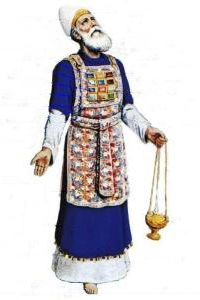
\includegraphics[width=50mm,scale=1.5]{Extras/Melchisedec.jpg}
\vspace{0.4in}  % Create a title for the document and write it in bold font
\LARGE{\textbf{\date}} % Again, do a line break
\linebreak 
% Create a subtitle \large{with Outlines, Statistics, Cross References, and Notes}
\vspace{0.5in}
\begin{flushleft}
\LARGE{Day \#29: Saturday, 29 January 2022   \\}\vspace{0.25in}
\LARGE{Exodus 34-36 Psalm 29 Proverb 29}
\end{flushleft}
\vspace{0.6in}
\bigskip

\normalsize{Xenia, Oh.\\}
\normalsize{created: \today}
\vspace{1.3in}

\end{flushright}
\end{titlepage}

%%%%%%%%%%%%
%%%%%%%%%%%%
%%%%%%%%%%%%

%\titleJE

\newpage 

\tableofcontents\hypertarget{TOC}{}
\listoffigures
\listoftables

\hyphenation{A-bim-e-lech bre-thren E-phra-im  Gib-e-o-nites Jer-u-sa-lem through-out Phil-i-stines The-o-phil-us Am-a-le-kites ven-geance Mesh-el-e-mi-ah onan-ism Phar-a-oh thoughts grev-ous-ness Hach-a-liah adul-ter-er Shad-rach}

%\fcolorbox{black}{bone}{TEXT}
%%%%%%%%%%%%%%%%% EXTRA COLORS
%%%%%%%%%%%%%%%%% EXTRA COLORS
%%%%%%%%%%%%%%%%% EXTRA COLORS
\definecolor{champagne}{rgb}{0.97,0.91,0.81}
\definecolor{bone}{rgb}{0.89,0.85,0.79}

\definecolor{ForestGreen}{rgb}{0.00,0.29,0.098}
\definecolor{GIVING}{cmyk}{1,0.0,0.72,.1}

\definecolor{MLPE}{cmyk}{1,1,0,.45}
\definecolor{SOCCER}{cmyk}{.77, 0, .42, .49}
\definecolor{PAYBILL}{cmyk}{0,0.83,0.76,0.07}
\definecolor{SERMON}{cmyk}{.14,.9,0,.30} % aka seance \href{http://www.flatuicolorpicker.com/purple-cmyk-color-model/}{seance}
\definecolor{BIBLE}{cmyk}{0,.17,.74,.17}
\definecolor{WORKBLUE}{cmyk}{1, .5, 0, .6}
\definecolor{myOrange}{cmyk}{0, .4, .98, .03}
\definecolor{myTan}{cmyk}{0.0,.07,.17,.10}
\definecolor{myRed}{cmyk}{0,1,1,0}
\definecolor{myWhite}{cmyk}{0,0,0,0}
\definecolor{BLUESoD}{cmyk}{.97,.84,0,.04}
\definecolor{WHITE}{cmyk}{0,0,0,0}
\definecolor{OLDGOLD}{cmyk}{0.05,0.3,1.00,0}
\definecolor{CASTLETON}{cmyk}{1,0,0.31,0.66}
\definecolor{cadmiumgreen}{rgb}{0.0, 0.42, 0.24}
\definecolor{jungle}{rgb}{0.203,0.4882,0.1718}
\definecolor{MYGOLD}{rgb}{1,.84,0}

\definecolor{MYLIGHTGRAY}{rgb}{.85,.85,.85}

\definecolor{codegreen}{rgb}{0,0.6,0}
\definecolor{codegray}{rgb}{0.5,0.5,0.5}
\definecolor{codepurple}{rgb}{0.58,0,0.82}
\definecolor{backcolour}{rgb}{0.95,0.95,0.92}



\mdfdefinestyle{MyFrame}{%
    linecolor=blue,
    outerlinewidth=2pt,
    roundcorner=5pt,
    innertopmargin=\baselineskip,
    innerbottommargin=\baselineskip,
    innerrightmargin=10pt,
    innerleftmargin=10pt,
    backgroundcolor=gray!25!white}


\mdfdefinestyle{MyFrame2}{%
    linecolor=black,
    outerlinewidth=2pt,
    roundcorner=5pt,
    innertopmargin=\baselineskip,
    innerbottommargin=\baselineskip,
    innerrightmargin=10pt,
    innerleftmargin=10pt,
    backgroundcolor=yellow!25!white}



%%%%%
%% for PFTTIS list
%%%%%

%%% And Joseph said unto
\index[PFTTIS]{And Joseph said unto!Genesis!Gen 40:008}
\index[PFTTIS]{And Joseph said unto!Genesis!Gen 40:012}
\index[PFTTIS]{And Joseph said unto!Genesis!Gen 41:025}
\index[PFTTIS]{And Joseph said unto!Genesis!Gen 42:014}
\index[PFTTIS]{And Joseph said unto!Genesis!Gen 42:018}
\index[PFTTIS]{And Joseph said unto!Genesis!Gen 44:015}
\index[PFTTIS]{And Joseph said unto!Genesis!Gen 45:003}
\index[PFTTIS]{And Joseph said unto!Genesis!Gen 45:004}
\index[PFTTIS]{And Joseph said unto!Genesis!Gen 46:031}
\index[PFTTIS]{And Joseph said unto!Genesis!Gen 48:009}
\index[PFTTIS]{And Joseph said unto!Genesis!Gen 48:018}
\index[PFTTIS]{And Joseph said unto!Genesis!Gen 50:019}
\index[PFTTIS]{And Joseph said unto!Genesis!Gen 50:024}


%%% a shadow
\index[PFTTIS]{a shadow!1Chronicles!1Chr 029:15}
\index[PFTTIS]{a shadow!Job!Job 008:09}
\index[PFTTIS]{a shadow!Job!Job 014:02}
\index[PFTTIS]{a shadow!Job!Job 017:07}
\index[PFTTIS]{a shadow!Psalm!Psa 102:011}
\index[PFTTIS]{a shadow!Psalm!Psa 144:004}
\index[PFTTIS]{a shadow!Ecclesiastes!Eccl 006:012}
\index[PFTTIS]{a shadow!Ecclesiastes!Eccl 008:013}
\index[PFTTIS]{a shadow!Isaiah!Isa 04:006}
\index[PFTTIS]{a shadow!Isaiah!Isa 25:004}
\index[PFTTIS]{a shadow!Jonah!Jnh 04:06}
\index[PFTTIS]{a shadow!Colossians!Col 02:017}
\index[PFTTIS]{a shadow!Hebews!Heb 10:001}

%%% blessed is the man
\index[PFTTIS]{blessed is the man!Psalm!Psa 001:001}
\index[PFTTIS]{blessed is the man!Psalm!Psa 032:002}
\index[PFTTIS]{blessed is the man!Psalm!Psa 034:008}
\index[PFTTIS]{blessed is the man!Psalm!Psa 065:004}
\index[PFTTIS]{blessed is the man!Psalm!Psa 084:005}
\index[PFTTIS]{blessed is the man!Psalm!Psa 084:012}
\index[PFTTIS]{blessed is the man!Psalm!Psa 094:012}
\index[PFTTIS]{blessed is the man!Psalm!Psa 112:001}
\index[PFTTIS]{blessed is the man!Proverbs!Pro 008:034}
\index[PFTTIS]{blessed is the man!Isaiah!Isa 056:002}
\index[PFTTIS]{blessed is the man!Jeremiah!Jer 017:007}
\index[PFTTIS]{blessed is the man!Romans!Rom 004:008}
\index[PFTTIS]{blessed is the man!James!Jam 001:012}


%%% carry them
\index[PFTTIS]{carry them!Leviticus!Lev 14:045}
\index[PFTTIS]{carry them!Numbers!Num 11:012}
\index[PFTTIS]{carry them!Joshua!Jsh 04:003}
\index[PFTTIS]{carry them!1Samuel!1Sam 20:040}
\index[PFTTIS]{carry them!1Kings!1Kng 08:046}
\index[PFTTIS]{carry them!2Chronicles!2Chr 06:036}
\index[PFTTIS]{carry them!Ezra!Ezra 05:015}
\index[PFTTIS]{carry them!Isaiah!Isa 40:011}
\index[PFTTIS]{carry them!Isaiah!Isa 41:016}
\index[PFTTIS]{carry them!Isaiah!Isa 57:013}
\index[PFTTIS]{carry them!Jeremiah!Jer 20:004}
\index[PFTTIS]{carry them!Jeremiah!Jer 20:005}
\index[PFTTIS]{carry them!Jeremiah!Jer 43:012}


\index[PFTTIS]{good tidings!2Samuel!2Sam 18:027}
\index[PFTTIS]{good tidings!1Kings!1Ki 01:042}
\index[PFTTIS]{good tidings!2Kings!2Ki 07:009 (2x)}
\index[PFTTIS]{good tidings!Isaiah!Isa 40:009 (2x)}
\index[PFTTIS]{good tidings!Isaiah!Isa 41:007}
\index[PFTTIS]{good tidings!Isaiah!Isa 52:007}
\index[PFTTIS]{good tidings!Isaiah!Isa 61:001}
\index[PFTTIS]{good tidings!Nahum!Nah 01:005}
\index[PFTTIS]{good tidings!Luke!Lk 02:010}
\index[PFTTIS]{good tidings!1Thessalonians!1Thess 03:006}


%%% dead body
\index[PFTTIS]{dead body!Leviticus!Lev 21:011}
\index[PFTTIS]{dead body!Numbers!Num 06:006}
\index[PFTTIS]{dead body!Numbers!Num 09:006}
\index[PFTTIS]{dead body!Numbers!Num 09:007}
\index[PFTTIS]{dead body!Numbers!Num 09:010}
\index[PFTTIS]{dead body!Numbers!Num 09:011}
\index[PFTTIS]{dead body!Numbers!Num 09:013}
\index[PFTTIS]{dead body!Numbers!Num 09:016}
\index[PFTTIS]{dead body!2Kings!2Ki 08:005}
\index[PFTTIS]{dead body!Isaiah!Isa 26:019}
\index[PFTTIS]{dead body!Jeremiah!Jer 26:023}
\index[PFTTIS]{dead body!Jeremiah!Jer 36:030}
\index[PFTTIS]{dead body!Haggai!Hag 02:013}

%%% great sea
\index[PFTTIS]{great sea!Numbers!Num 34:006}
\index[PFTTIS]{great sea!Numbers!Num 34:007}
\index[PFTTIS]{great sea!Joshua!Jos 01:004}
\index[PFTTIS]{great sea!Joshua!Jos 09:001}
\index[PFTTIS]{great sea!Joshua!Jos 15:012}
\index[PFTTIS]{great sea!Joshua!Jos 15:047}
\index[PFTTIS]{great sea!Joshua!Jos 23:004}
\index[PFTTIS]{great sea!Ezekiel!Eze 47:010}
\index[PFTTIS]{great sea!Ezekiel!Eze 47:015}
\index[PFTTIS]{great sea!Ezekiel!Eze 47:019}
\index[PFTTIS]{great sea!Ezekiel!Eze 47:020}
\index[PFTTIS]{great sea!Ezekiel!Eze 48:028}
\index[PFTTIS]{great sea!Daniel!Dan 07:002}


%%% have forsaken me
\index[PFTTIS]{have forsaken me!Judges!Jdg 10:013}
\index[PFTTIS]{have forsaken me!1Samuel!1Sam 08:008}
\index[PFTTIS]{have forsaken me!1Kings!1Ki 11:033}
\index[PFTTIS]{have forsaken me!2Kings!2Ki 22:017}
\index[PFTTIS]{have forsaken me!2Chronicles!2Chr 12:005}
\index[PFTTIS]{have forsaken me!2Chronicles!2Chr 34:025}
\index[PFTTIS]{have forsaken me!Jeremiah!Jer 01:016}
\index[PFTTIS]{have forsaken me!Jeremiah!Jer 02:013}
\index[PFTTIS]{have forsaken me!Jeremiah!Jer 05:007}
\index[PFTTIS]{have forsaken me!Jeremiah!Jer 05:019}
\index[PFTTIS]{have forsaken me!Jeremiah!Jer 16:011 (2x)}
\index[PFTTIS]{have forsaken me!Jeremiah!Jer 19:004}

%%% no king
\index[PFTTIS]{no king!Judges!Jdg 17:06}
\index[PFTTIS]{no king!Judges!Jdg 18:01}
\index[PFTTIS]{no king!Judges!Jdg 19:01}
\index[PFTTIS]{no king!Judges!Jdg 21:25}
\index[PFTTIS]{no king!1Kings!1Ki 22:47}
\index[PFTTIS]{no king!2Kings!2Ki 23:25}
\index[PFTTIS]{no king!Nehemiah!Neh 13:26}
\index[PFTTIS]{no king!Psalms!Psa 033:016}
\index[PFTTIS]{no king!Proverbs!Pro 30:27}
\index[PFTTIS]{no king!Daniel!Dan 02:10}
\index[PFTTIS]{no king!Hosea!Hos 10:03}
\index[PFTTIS]{no king!Micah!Mic 04:09}
\index[PFTTIS]{no king!John!Jhn 19:15}


%%% rebellious house
\index[PFTTIS]{rebellious house!Exodus!Exo 02:005}
\index[PFTTIS]{rebellious house!Exodus!Exo 02:006}
\index[PFTTIS]{rebellious house!Exodus!Exo 02:008}
\index[PFTTIS]{rebellious house!Exodus!Exo 03:009}
\index[PFTTIS]{rebellious house!Exodus!Exo 03:026}
\index[PFTTIS]{rebellious house!Exodus!Exo 03:027}
\index[PFTTIS]{rebellious house!Exodus!Exo 12:002 (2x)}
\index[PFTTIS]{rebellious house!Exodus!Exo 12:003}
\index[PFTTIS]{rebellious house!Exodus!Exo 12:009}
\index[PFTTIS]{rebellious house!Exodus!Exo 12:025}
\index[PFTTIS]{rebellious house!Exodus!Exo 17:012}
\index[PFTTIS]{rebellious house!Exodus!Exo 24:003}

%%% seek him
\index[PFTTIS]{seek him!Deuteronomy!Deu 04:029}\index[PFTTIS]{seek him!1Samuel!1Sam 23:025}
\index[PFTTIS]{seek him!1Chronicles!1Chr 28:009}
\index[PFTTIS]{seek him!2Chronicles!1Chr 15:002}
\index[PFTTIS]{seek him!Ezra!Ezr 08:022}
\index[PFTTIS]{seek him!Psalms!Psa 022:026}
\index[PFTTIS]{seek him!Psalms!Psa 024:006}
\index[PFTTIS]{seek him!Psalms!Psa 119:002}
\index[PFTTIS]{seek him!SoS!SoS 03:002}
\index[PFTTIS]{seek him!SoS!SoS 06:001}
\index[PFTTIS]{seek him!Hosea!Hos 07:010}
\index[PFTTIS]{seek him!Amos!Amo 05:008}
\index[PFTTIS]{seek him!Hebrews!Heb 11:0063}


%%% seek ye
\index[PFTTIS]{seek ye!Isaiah!Isa 34:016}
\index[PFTTIS]{seek ye!Isaiah!Isa 45:019}
\index[PFTTIS]{seek ye!Isaiah!Isa 55:006}
\index[PFTTIS]{seek ye!Amos!Amos 5:004}
\index[PFTTIS]{seek ye!John!John 1:38}
\index[PFTTIS]{seek ye!John!John 18:4}
\index[PFTTIS]{seek ye!John!John 18:7}
\index[PFTTIS]{seek ye!Matthew!Matt 6:33}
\index[PFTTIS]{seek ye!Numbers!Num 16:10}
\index[PFTTIS]{seek ye!Luke!Luke 12:31}
\index[PFTTIS]{seek ye!Luke!Luke 24:5}
\index[PFTTIS]{seek ye!Psalm!Psa 27:8}
\index[PFTTIS]{seek ye!Zephaniah!Zeph 2:3}

%%% the uncircumcised
\index[PFTTIS]{the uncircumcised!Genesis!Gen 17:014}
\index[PFTTIS]{the uncircumcised!Judges!Jdg 14:003}
\index[PFTTIS]{the uncircumcised!Judges!Jdg 15:018}
\index[PFTTIS]{the uncircumcised!2Samuel!2Sam 01:020}
\index[PFTTIS]{the uncircumcised!Isaiah!Isa 02:001}
\index[PFTTIS]{the uncircumcised!Jeremiah!Jer 09:025}
\index[PFTTIS]{the uncircumcised!Ezekiel!Eze 28:010}
\index[PFTTIS]{the uncircumcised!Ezekiel!Eze 31:018}
\index[PFTTIS]{the uncircumcised!Ezekiel!Eze 32:019}
\index[PFTTIS]{the uncircumcised!Ezekiel!Eze 32:027}
\index[PFTTIS]{the uncircumcised!Ezekiel!Eze 32:028}
\index[PFTTIS]{the uncircumcised!Ezekiel!Eze 32:029}
\index[PFTTIS]{the uncircumcised!Ezekiel!Eze 32:032}

%%% worship him
\index[PFTTIS]{worship him!Psalms!Psa 97:007}
\index[PFTTIS]{worship him!Zephaniah!Zeph 02:011}
\index[PFTTIS]{worship him!Matthew!Matt 02:002}
\index[PFTTIS]{worship him!Matthew!Matt 02:008}
\index[PFTTIS]{worship him!John!John 04:023}
\index[PFTTIS]{worship him!John!John 04:024 (2x)} 
\index[PFTTIS]{worship him!Acts!Acts 17:023}
\index[PFTTIS]{worship him!Hebrews!Heb 01:006}
\index[PFTTIS]{worship him!Revelation!Rev 04:010}
\index[PFTTIS]{worship him!Revelation!Rev 13:008}
\index[PFTTIS]{worship him!Revelation!Rev 14:007}
\index[PFTTIS]{worship him!Revelation!Rev 19:010}


%%%%%
%% for PFTTIS list
%%%%%

%%% afflictions
\index[WFTTIS]{afflictions!Psalms!Psa 34:019}
\index[WFTTIS]{afflictions!Psalms!Psa 132:001}
\index[WFTTIS]{afflictions!Acts!Acts 07:010}
\index[WFTTIS]{afflictions!Acts!Acts 20:023}
\index[WFTTIS]{afflictions!2Corinthians!2Cor 06:004}
\index[WFTTIS]{afflictions!Colossians!Col 01:024}
\index[WFTTIS]{afflictions!1Thessalonians!1Thess 03:003}
\index[WFTTIS]{afflictions!2Timothy!2Tim 01:008}
\index[WFTTIS]{afflictions!2Timothy!2Tim 03:011}
\index[WFTTIS]{afflictions!2Timothy!2Tim 04:005}
\index[WFTTIS]{afflictions!Hebrews!Heb 10:032}
\index[WFTTIS]{afflictions!Hebrews!Heb 10:033}
\index[WFTTIS]{afflictions!1Peter!1Pet 05:009}

%%% acsend
\index[WFTTIS]{acsend!Joshua!Jos 06:05}
\index[WFTTIS]{acsend!Psalm!Psa 024:003}
\index[WFTTIS]{acsend!Psalm!Psa 135:007}
\index[WFTTIS]{acsend!Psalm!Psa 139:008}
\index[WFTTIS]{acsend!Isaiah!Isa 14:013}
\index[WFTTIS]{acsend!Isaiah!Isa 14:014}
\index[WFTTIS]{acsend!Jeremiah!Jer 10:013}
\index[WFTTIS]{acsend!Jeremiah!Jer 51:016}
\index[WFTTIS]{acsend!Ezekiel!Eze 38:009}
\index[WFTTIS]{acsend!John!John 06:062}
\index[WFTTIS]{acsend!John!John 20:017}
\index[WFTTIS]{acsend!Romans!Rom 10:006}
\index[WFTTIS]{acsend!Revelation!Rev 17:008}

%%% Assyrian
\index[WFTTIS]{Assyrian!Isaiah!Isa 10:005}
\index[WFTTIS]{Assyrian!Isaiah!Isa 10:024}
\index[WFTTIS]{Assyrian!Isaiah!Isa 14:025}
\index[WFTTIS]{Assyrian!Isaiah!Isa 19:023}
\index[WFTTIS]{Assyrian!Isaiah!Isa 23:013}
\index[WFTTIS]{Assyrian!Isaiah!Isa 30:031}
\index[WFTTIS]{Assyrian!Isaiah!Isa 31:008}
\index[WFTTIS]{Assyrian!Isaiah!Isa 52:004}
\index[WFTTIS]{Assyrian!Ezekiel!Eze 31:003}
\index[WFTTIS]{Assyrian!Hosea!Hos 05:013}
\index[WFTTIS]{Assyrian!Hosea!Hos 11:005}
\index[WFTTIS]{Assyrian!Micah!Hos 05:005}
\index[WFTTIS]{Assyrian!Micah!Hos 05:006}

%%% blot
\index[WFTTIS]{blot!Exodus!Exo 32:032}
\index[WFTTIS]{blot!Exodus!Exo 32:033}
\index[WFTTIS]{blot!Numbers!Num 05:026}
\index[WFTTIS]{blot!Deuteronomy!Deut 09:014}
\index[WFTTIS]{blot!Deuteronomy!Deut 25:019}
\index[WFTTIS]{blot!Deuteronomy!Deut 29:020}
\index[WFTTIS]{blot!2Kings!2Ki 14:027}
\index[WFTTIS]{blot!Job!Job 31:007}
\index[WFTTIS]{blot!Psalms!Psa 51:001}
\index[WFTTIS]{blot!Psalms!Psa 51:009}
\index[WFTTIS]{blot!Proverbs!Pro 09:007}
\index[WFTTIS]{blot!Jeremiah!Jer 18:023}
\index[WFTTIS]{blot!Revelation!Rev 03:005}


%%% chain
\index[WFTTIS]{chain!Genesis!Gen 41:042}
\index[WFTTIS]{chain!1Kings!1Ki 07:017}
\index[WFTTIS]{chain!Psalms!Psa 73:006}
\index[WFTTIS]{chain!SoS!Sos 04:009}
\index[WFTTIS]{chain!Lamentations!Lam 03:007}
\index[WFTTIS]{chain!Ezekiel!Eze 07:023}
\index[WFTTIS]{chain!Ezekiel!Eze 16:011}
\index[WFTTIS]{chain!Daniel!Dan 05:007}
\index[WFTTIS]{chain!Daniel!Dan 05:016}
\index[WFTTIS]{chain!Daniel!Dan 05:029}
\index[WFTTIS]{chain!Acts!Acts 28:020}
\index[WFTTIS]{chain!2Timothy!2Tim 01:016}
\index[WFTTIS]{chain!Revelation!Rev 20:001}


%%% controversy
\index[WFTTIS]{controversy!Deuteronomy!Deu 17:008}
\index[WFTTIS]{controversy!Deuteronomy!Deu 19:017}
\index[WFTTIS]{controversy!Deuteronomy!Deu 21:005}
\index[WFTTIS]{controversy!Deuteronomy!Deu 25:001}
\index[WFTTIS]{controversy!2Samuel!2Sam 15:002}
\index[WFTTIS]{controversy!Isaiah!Isa 34:008}
\index[WFTTIS]{controversy!Jeremiah!Jer 25:031}
\index[WFTTIS]{controversy!Ezekiel!Eze 44:024}
\index[WFTTIS]{controversy!Hosea!Hos 04:001}
\index[WFTTIS]{controversy!Hosea!Hos 12:002}
\index[WFTTIS]{controversy!Micah!Mic 06:002 (2x)}
\index[WFTTIS]{controversy!1Timothy!1Tim 03:016}


%%% Dagon/Dagon's
\index[WFTTIS]{Dagon!Judges!Jdg 16:023}
\index[WFTTIS]{Dagon!1Samuel!1Sam 05:002 (2x)}
\index[WFTTIS]{Dagon!1Samuel!1Sam 05:003 (2x)}
\index[WFTTIS]{Dagon!1Samuel!1Sam 05:004 (3x)}
\index[WFTTIS]{Dagon!1Samuel!1Sam 05:005 (3x)}
\index[WFTTIS]{Dagon!1Samuel!1Sam 05:007}
\index[WFTTIS]{Dagon!1Chronicles!1Chr 10:010}

%%% disobedient
\index[WFTTIS]{disobedient!1Kings!1Ki 13:026}
\index[WFTTIS]{disobedient!Nehemiah!Neh 09:026}
\index[WFTTIS]{disobedient!Luke!Luke 01:017}
\index[WFTTIS]{disobedient!Acts!Acts 26:019}
\index[WFTTIS]{disobedient!Romans!Rom 01:030}
\index[WFTTIS]{disobedient!Romans!Rom 10:021}
\index[WFTTIS]{disobedient!1Timothy!1Tim 01:009}
\index[WFTTIS]{disobedient!2Timothy!2Tim 03:002}
\index[WFTTIS]{disobedient!Titus!Titus 01:016}
\index[WFTTIS]{disobedient!Titus!Titus 03:003}
\index[WFTTIS]{disobedient!1Peter!1Pet 02:007}
\index[WFTTIS]{disobedient!1Peter!1Pet 02:008}
\index[WFTTIS]{disobedient!1Peter!1Pet 03:020}


%%% doubt
\index[WFTTIS]{doubt!Genesis!Gen 37:033}
\index[WFTTIS]{doubt!Deuteronomy!Deu 28:066}
\index[WFTTIS]{doubt!Job!Job 12:002}
\index[WFTTIS]{doubt!Matthew!Matt 14:031}
\index[WFTTIS]{doubt!Matthew!Matt 21:021}
\index[WFTTIS]{doubt!Mark!Mk 11:023}
\index[WFTTIS]{doubt!Luke!Lk 11:020}
\index[WFTTIS]{doubt!John!Jhn 10:024}
\index[WFTTIS]{doubt!Acts!Acts 02:012}
\index[WFTTIS]{doubt!Acts!Acts 28:004}
\index[WFTTIS]{doubt!1Corinthians!1Cor 09:010}
\index[WFTTIS]{doubt!Galatians!Gal 04:020}
\index[WFTTIS]{doubt!1John!1Jhn 02:019}


%%% dungeon
\index[WFTTIS]{dungeon!Genesis!Gen 40:015}
\index[WFTTIS]{dungeon!Genesis!Gen 41:014}
\index[WFTTIS]{dungeon!Exodus!Exo 12:029}
\index[WFTTIS]{dungeon!Jeremiah!Jer 37:016}
\index[WFTTIS]{dungeon!Jeremiah!Jer 38:006 (2x)}
\index[WFTTIS]{dungeon!Jeremiah!Jer 38:007}
\index[WFTTIS]{dungeon!Jeremiah!Jer 38:009}
\index[WFTTIS]{dungeon!Jeremiah!Jer 38:010}
\index[WFTTIS]{dungeon!Jeremiah!Jer 38:011}
\index[WFTTIS]{dungeon!Jeremiah!Jer 38:013}
\index[WFTTIS]{dungeon!Lamentations!Lam 03:053}
\index[WFTTIS]{dungeon!Lamentations!Lam 03:055}


%%% error
\index[WFTTIS]{error!2Samuel!2Sam 06:007}
\index[WFTTIS]{error!Job!Job 19:004}
\index[WFTTIS]{error!Ecclesiastes!Ecc 05:006}
\index[WFTTIS]{error!Ecclesiastes!Ecc 10:005}
\index[WFTTIS]{error!Isaiah!Isa 32:006}
\index[WFTTIS]{error!Daniel!Dan 06:004}
\index[WFTTIS]{error!Matthew!Matt 27:064}
\index[WFTTIS]{error!Romans!Rom 01:027}
\index[WFTTIS]{error!James!Jam 05:020}
\index[WFTTIS]{error!2Peter!2Pet 02:018}
\index[WFTTIS]{error!2Peter!2Pet 03:017}
\index[WFTTIS]{error!1John!1Jn 04:006}
\index[WFTTIS]{error!Jude!Jude 01:011}

%%% fourish
\index[WFTTIS]{fourish!Psalms!Psa 072:007}
\index[WFTTIS]{fourish!Psalms!Psa 072:016}
\index[WFTTIS]{fourish!Psalms!Psa 092:007}
\index[WFTTIS]{fourish!Psalms!Psa 092:012}
\index[WFTTIS]{fourish!Psalms!Psa 092:013}
\index[WFTTIS]{fourish!Psalms!Psa 132:018}
\index[WFTTIS]{fourish!Proverbs!Pro 11:28}
\index[WFTTIS]{fourish!Proverbs!Pro 14:11}
\index[WFTTIS]{fourish!Ecclesiastes!Ecc 12:05}
\index[WFTTIS]{fourish!SongOfSolomon!SOS 07:12}
\index[WFTTIS]{fourish!Isaiah!Isa 17:11}
\index[WFTTIS]{fourish!Isaiah!Isa 66:14}
\index[WFTTIS]{fourish!Ezekiel!Eze 17:24}




%%% giants
\index[WFTTIS]{giants!Genesis!Gen 06:004}
\index[WFTTIS]{giants!Numbers!Num 13:033}
\index[WFTTIS]{giants!Deuteronomy!Deut 02:011}
\index[WFTTIS]{giants!Deuteronomy!Deut 02:021}
\index[WFTTIS]{giants!Deuteronomy!Deut 03:011}
\index[WFTTIS]{giants!Deuteronomy!Deut 03:013}
\index[WFTTIS]{giants!Joshua!Josh 12:004}
\index[WFTTIS]{giants!Joshua!Josh 13:012}
\index[WFTTIS]{giants!Joshua!Josh 15:008}
\index[WFTTIS]{giants!Joshua!Josh 17:015}
\index[WFTTIS]{giants!Joshua!Josh 16:016}

%%% good man
\index[WFTTIS]{good man!2 Samuel!2Sa 18:27}
%(1) Psalms 37:23 [5]
%(1) Psalms 112:5 [2]
%(1) Proverbs 12:2 [2]
%(1) Proverbs 13:22 [2]
%(1) Proverbs 14:14 [14]
%(1) Micah 7:2 [2]
%(1) Matthew 12:35 [2]
%(1) Luke 6:45 [2]
%(1) Luke 23:50 [15]
%(1) John 7:12 [17]
%(1) Acts 11:24 [5]
%(1) Romans 5:7 [14]

%%% Hinnom
\index[WFTTIS]{Hinnom!Joshua!Jsh 15:008}
\index[WFTTIS]{Hinnom!Joshua!Jsh 18:016}
\index[WFTTIS]{Hinnom!2Kings!2Ki 23:010}
\index[WFTTIS]{Hinnom!2Chronicles!2Chr 28:003}
\index[WFTTIS]{Hinnom!2Chronicles!2Chr 33:006}
\index[WFTTIS]{Hinnom!Nehemiah!Neh 11:030}
\index[WFTTIS]{Hinnom!Jeremiah!Jer 07:031}
\index[WFTTIS]{Hinnom!Jeremiah!Jer 07:032}
\index[WFTTIS]{Hinnom!Jeremiah!Jer 19:002}
\index[WFTTIS]{Hinnom!Jeremiah!Jer 19:006}
\index[WFTTIS]{Hinnom!Jeremiah!Jer 32:035}

%%% inclined
\index[WFTTIS]{inclined!Judges!Jdg 09:003}
\index[WFTTIS]{inclined!Psalms!Psa 040:001}
\index[WFTTIS]{inclined!Psalms!Psa 116:002}
\index[WFTTIS]{inclined!Psalms!Psa 119:112}
\index[WFTTIS]{inclined!Proverbs!Pro 05:13}
\index[WFTTIS]{inclined!Jeremiah!Jer 07:24}
\index[WFTTIS]{inclined!Jeremiah!Jer 07:26}
\index[WFTTIS]{inclined!Jeremiah!Jer 11:08}
\index[WFTTIS]{inclined!Jeremiah!Jer 17:23}
\index[WFTTIS]{inclined!Jeremiah!Jer 25:04}
\index[WFTTIS]{inclined!Jeremiah!Jer 34:14}
\index[WFTTIS]{inclined!Jeremiah!Jer 35:15}
\index[WFTTIS]{inclined!Jeremiah!Jer 44:05}


%%% laughed
\index[WFTTIS]{laughed!Genesis!Gen 17:017}
\index[WFTTIS]{laughed!Genesis!Gen 18:012}
\index[WFTTIS]{laughed!Genesis!Gen 18:015}
\index[WFTTIS]{laughed!2Kings!2Ki 19:021}
\index[WFTTIS]{laughed!2Chronicles!2Chr 30:010}
\index[WFTTIS]{laughed!Nehemiah!Neh 02:019}
\index[WFTTIS]{laughed!Job!Job 12:004}
\index[WFTTIS]{laughed!Job!Job 29:024}
\index[WFTTIS]{laughed!Isaiah!Isa 37:022}
\index[WFTTIS]{laughed!Ezekiel!Ezek 23:032}
\index[WFTTIS]{laughed!Matthew!Matt 09:024}
\index[WFTTIS]{laughed!Mark!Mk 05:040}
\index[WFTTIS]{laughed!Luke!Lk 08:053}

%%% liar
\index[WFTTIS]{liar!Job!Job 24:025}
\index[WFTTIS]{liar!Proverbs!Pro 17:004}
\index[WFTTIS]{liar!Proverbs!Pro 19:022}
\index[WFTTIS]{liar!Proverbs!Pro 30:006}
\index[WFTTIS]{liar!Jeremiah!Jer 15:018}
\index[WFTTIS]{liar!John!Jhn 08:044}
\index[WFTTIS]{liar!John!Jhn 08:055}
\index[WFTTIS]{liar!Romans!Rom 03:004}
\index[WFTTIS]{liar!1John!1Jhn 01:010}
\index[WFTTIS]{liar!1John!1Jhn 02:004}
\index[WFTTIS]{liar!1John!1Jhn 02:022}
\index[WFTTIS]{liar!1John!1Jhn 04:020}
\index[WFTTIS]{liar!1John!1Jhn 05:010}

%%% palsy
\index[WFTTIS]{palsy!Matthew!Matt 04:024}
\index[WFTTIS]{palsy!Matthew!Matt 08:006}
\index[WFTTIS]{palsy!Matthew!Matt 09:002}
\index[WFTTIS]{palsy!Matthew!Matt 09:006}
\index[WFTTIS]{palsy!Mark!Mk 02:003}
\index[WFTTIS]{palsy!Mark!Mk 02:004}
\index[WFTTIS]{palsy!Mark!Mk 02:005}
\index[WFTTIS]{palsy!Mark!Mk 02:009}
\index[WFTTIS]{palsy!Mark!Mk 02:010}
\index[WFTTIS]{palsy!Luke!Lk 05:018}
\index[WFTTIS]{palsy!Luke!Lk 05:024}
\index[WFTTIS]{palsy!Acts!Acts 09:033}

%%% Profitable
\index[WFTTIS]{profitable!Job!Job 22:002 (2x)}
\index[WFTTIS]{profitable!Ecclesiastes!Ecc 10:010}
\index[WFTTIS]{profitable!Isaiah!Isa 44:010}
\index[WFTTIS]{profitable!Jeremiah!Jer 13:007}
\index[WFTTIS]{profitable!Matthew!Matt 05:029}
\index[WFTTIS]{profitable!Matthew!Matt 05:030}
\index[WFTTIS]{profitable!Acts!Acts 20:020}
\index[WFTTIS]{profitable!1Timothy!1Tim 04:008}
\index[WFTTIS]{profitable!2Timothy!2Tim 03:016}
\index[WFTTIS]{profitable!2Timothy!2Tim 04:011}
\index[WFTTIS]{profitable!Titus!Titus 03:008}
\index[WFTTIS]{profitable!Philemon!Phlm 01:011}

%%% Rechab
\index[WFTTIS]{Rechab!2Samuel!2Sam 04:002}
\index[WFTTIS]{Rechab!2Samuel!2Sam 04:005}
\index[WFTTIS]{Rechab!2Samuel!2Sam 04:006}
\index[WFTTIS]{Rechab!2Samuel!2Sam 04:009}
\index[WFTTIS]{Rechab!2KIngs!2Ki 10:015}
\index[WFTTIS]{Rechab!2KIngs!2Ki 10:023}
\index[WFTTIS]{Rechab!1Chronicles!1Chr 02:055}
\index[WFTTIS]{Rechab!Nehemiah!Neh 03:014}
\index[WFTTIS]{Rechab!Jeremiah!Jer 35:006}
\index[WFTTIS]{Rechab!Jeremiah!Jer 35:008}
\index[WFTTIS]{Rechab!Jeremiah!Jer 35:014}
\index[WFTTIS]{Rechab!Jeremiah!Jer 35:016}
\index[WFTTIS]{Rechab!Jeremiah!Jer 35:019}

%%% serpents
\index[WFTTIS]{serpents!Exodus!Exo 07:012}
\index[WFTTIS]{serpents!Numbers!Num 21:006}
\index[WFTTIS]{serpents!Numbers!Num 21:007}
\index[WFTTIS]{serpents!Deuteronomy!Deu 08:015}
\index[WFTTIS]{serpents!Deuteronomy!Deu 32:024}
\index[WFTTIS]{serpents!Jeremiah!Jer 08:017}
\index[WFTTIS]{serpents!Matthew!Matt 10:016}
\index[WFTTIS]{serpents!Matthew!Matt 23:033}
\index[WFTTIS]{serpents!Mark!Mk 16:018}
\index[WFTTIS]{serpents!Luke!Lk 10:019}
\index[WFTTIS]{serpents!1Corinthians!1Cor 10:009}
\index[WFTTIS]{serpents!James!Jas 03:007}
\index[WFTTIS]{serpents!Revelation!Rev 09:019}

%%% short
\index[WFTTIS]{short!Numbers!Num 11:023}
\index[WFTTIS]{short!2Kings!2Ki 10:032}
\index[WFTTIS]{short!Job!Job 17:012}
\index[WFTTIS]{short!Job!Job 20:005}
\index[WFTTIS]{short!Psalms!Psa 89:047}
\index[WFTTIS]{short!Romans!Rom 03:023}
\index[WFTTIS]{short!Romans!Rom 09:028  (2x)}
\index[WFTTIS]{short!1Corinthians!1Cor 07:029}
\index[WFTTIS]{short!1Thessalonians!1Thess 02:017}
\index[WFTTIS]{short!Hebrews!Heb 04:001}
\index[WFTTIS]{short!Revelation!Rev 12:012}
\index[WFTTIS]{short!Revelation!Rev 17:010}

%%% smiteth
\index[WFTTIS]{smiteth!Exodus!Exo 21:012}
\index[WFTTIS]{smiteth!Exodus!Exo 21:15}
\index[WFTTIS]{smiteth!Deuteronomy!Dt 25:11}
\index[WFTTIS]{smiteth!Deuteronomy!Dt 27:24}
\index[WFTTIS]{smiteth!Joshua!Jsh 15:16}
\index[WFTTIS]{smiteth!Judges!Jdg 15:16}
\index[WFTTIS]{smiteth!2 Samuel!2Sa 05:08}
\index[WFTTIS]{smiteth!1Chronicles!1Chr 11:06}
\index[WFTTIS]{smiteth!Job!1Chr 26:12}
\index[WFTTIS]{smiteth!Isaiah!Isa 09:13}
\index[WFTTIS]{smiteth!Lamentations!Lam 03:30}
\index[WFTTIS]{smiteth!Ezekiel!Eze 07:09}
\index[WFTTIS]{smiteth!Luke!Lk 06:29}



%%% vanities
\index[WFTTIS]{vanities!Deuteronomy!Deut 21:021}
\index[WFTTIS]{vanities!1Kings!1Ki 16:013}
\index[WFTTIS]{vanities!1Kings!1Ki 16:026}
\index[WFTTIS]{vanities!Psalms!Psa 031:006}
\index[WFTTIS]{vanities!Ecclesiastes!Ecc 01:002 (2x)}
\index[WFTTIS]{vanities!Ecclesiastes!Ecc 05:007}
\index[WFTTIS]{vanities!Ecclesiastes!Ecc 12:008}
\index[WFTTIS]{vanities!Jeremiah!Jer 08:019}
\index[WFTTIS]{vanities!Jeremiah!Jer 10:008}
\index[WFTTIS]{vanities!Jeremiah!Jer 14:022}
\index[WFTTIS]{vanities!Jonah!Jnh 02:008}
\index[WFTTIS]{vanities!Acts!Acts 14:015}



%%%%%
%% for PFTTIS list
%%%%%

%%% worm
\index[WFITV]{worm!Exodus!Exo 16:024}
\index[WFITV]{worm!Job!Job 17:014}
\index[WFITV]{worm!Job!Job 24:029}
\index[WFITV]{worm!Job!Job 25:005 (2x)}
\index[WFITV]{worm!Psalms!Psa 022:006}
\index[WFITV]{worm!Isaiah!Isa 14:011}
\index[WFITV]{worm!Isaiah!Isa 41:014}
\index[WFITV]{worm!Isaiah!Isa 51:008}
\index[WFITV]{worm!Isaiah!Isa 66:024}
\index[WFITV]{worm!Jonah!Jnh 04:007}
\index[WFITV]{worm!Mark!Mk 09:044}
\index[WFITV]{worm!Mark!Mk 09:046}
\index[WFITV]{worm!Mark!Mk 09:048}


%\subsubsection{Title}
%\textbf{Introduction:} Isaiah 46 
%\index[speaker]{Speaker!Isaiah 49 (Title}
%\index[series]{Book (Speaker)!IPassage (Title)}
%\index[date]{2017/07/09!Isaiah 49 (Title)}
%\begin{compactenum}[I.]
%    \item  \textbf{Point} \index[scripture]{Isaiah!IPassage} (IPassage)
%\end{compactenum}




  

\chapter{Today's Readings}

\normalsize
 
\begin{center}
\begin{longtable}{|p{0.45in}|p{0.25in}|p{0.4in}|p{2.8in}|c|c|}
\caption[Today's Chapters]{Today's Chapters}\label{table:Today's Chapters} \\
\hline 
\multicolumn{1}{|c|}{\textbf{Chap}} & 
\multicolumn{1}{|c|}{\textbf{\#}} & 
\multicolumn{1}{|c|}{\textbf{Rvrs} } & 
\multicolumn{1}{|c|}{\textbf{address numerics}} & 
\multicolumn{1}{|c|}{\textbf{Vss}} & 
\multicolumn{1}{|c|}{\textbf{wds}}  \\ 
\hline 
\endfirsthead

 
\multicolumn{6}{c}
{{\bfseries \tablename\ \thetable{} -- continued from previous page}} \\  
\hline \multicolumn{1}{|c|}{\textbf{Chap}} & \multicolumn{1}{|c|}{\textbf{\#}} & \multicolumn{1}{|c|}{\textbf{Rev}} & \multicolumn{1}{|c|}{\textbf{addr Num}} & \multicolumn{1}{|c|}{\textbf{Verses}} & \multicolumn{1}{|c|}{\textbf{words}}  \\ \hline \endhead
 
%\hline \multicolumn{6}{|r|}{{Continued}} \\ \hline
\endfoot 
%Exo 20 & 70 & 1120 & 70 = 2 * 5 * 7; 1120 = 2 * 2 * 2 * 2 * 2 * 5 * 7 & 26 & 561 \\ \hline
%Exo 21 & 71 & 1119 & 71 is prime; 1119 = 3 * 373 & 36 & 893 \\ \hline \hline
%Exo 22 & 72 & 1118 &72 = 2 * 2 * 3 * 3; 1118 = 2 * 13 * 17 & 31 & 790 \\ \hline
%Exo 23 & 73 & 1117 & 73 is prime; 1117 is & 33 & 827 \\ \hline
%Exo 24 & 74 & 1116 & 74 = 2 * 37; 1116 = 2 8 2 * 3 * 3 * 31 & 18 & 492 \\ \hline \hline
%Exo 25 & 75 & 1115 & 75 = 3 * 5 * 5; 1115 = 5 * 223 & 40 & 926 \\ \hline
%Exo 26 & 76 & 1114 & 76 = 2 * 2 * 19; 1114 = 2 * 557 & 37 & 937 \\ \hline
%Exo 27 & 77 & 1113 & 77 = 7 * 11; 1113 = 3 * 7 * 53 & 18 & 492 \\ \hline \hline
%Exo 28 & 78 & 1112 & 78 = 2 * 3 * 13; 1112 = 2 * 2 * 2 * 139 & 43 & 1235 \\ \hline
%Exo 28 & 79 & 1111 & 79 is prime; 1111 = 11 * 101 & 46 & 1341 \\ \hline
%Exo 30 & 80 & 1110 & 80 = 2 * 2 * 2 * 2 * 5; 1110 = 2 * 3 * 5 * 37 & 38 & 970 \\ \hline \hline
%Exo 31 & 81 & 1109 & 81 = 3 * 3 * 3 * 3; 1109 is prime & 18 & 438 \\ \hline
%Exo 32 & 82 & 1108 & 82 = 1 * 41; 1108 = 2 * 2 * 277 & 35 & 1093 \\ \hline
%Exo 33 & 83 & 1107 & 83 is prime; 1107 = 3 * 3 * 3 * 41  & 23 & 710 \\ \hline \hline
Exo 34 & 84 & 1106 & 84 = 2 * 2 * 3 * 7; 1106 = 3 * 7 * 79 & 18 & 438 \\ \hline
Exo 35 & 85 & 1105 & 85 = 5 * 17; 1105 = 5 * 13 * 17 & 35 & 1093 \\ \hline
Exo 36 & 86 & 1104 & 86 = 2 * 43; 1104 = 2 * 2 * 2 * 2 * 3 * 23 & 23 & 710 \\ \hline \hline

%Psa 23 & 501 & 690 & 501 is prime; 690 = 2 * 3 * 5 * 23 & 31 & 246 \\ \hline \hline
%Psa 24 & 502 & 689 & 502 = 2 * 251 ; 689  = 13 * 53 & 10 & 178 \\ \hline \hline
%Psa 25 & 503 & 688 &  503 is prime ; 688  = 2 * 2 * 2 * 2 * 43 & 22 & 342 \\ \hline 
%Psa 27 & 504 & 687 &  504 = 2 * 2 * 2 * 3 * 3 * 7 ; 687  = 3 * 229 & 14 & 340 \\ \hline \hline
%Psa 28 & 505 & 686 &  505 = 5 * 101 ; 686  = 2 * 7 * 7 * 7 & 9 & 201 \\ \hline \hline
Psa 29 & 506 & 685 &  506 = 2 * 11 * 23 ; 685 = 5 * 137 & 11 & 179 \\ \hline \hline

%Pro 23 & 651 & 539 & 651 = 3 * 7 * 31; 539 = 7 * 7 * 11 & 35 & 566 \\ \hline \hline
%Pro 24 & 652 & 538 & 652 = 2 * 2 * 163; 538 = 2 * 269 & 34 & 580 \\ \hline \hline
%Pro 25 & 653 & 537 & 653 is prime; 537 = 3 * 179 & 28 & 522 \\ \hline \hline
%Pro 27 & 654 & 536 & 654 = 2 * 3 * 109; 536 = 2 * 2 * 2 * 67 & 23 & 460 \\ \hline 
%Pro 28 & 655 & 535 & 655 = 5 * 131; 535 = 5 * 107& 28 & 527 \\ \hline 
Pro 29 & 656 & 534 & 656 = 2 * 2 * 2 * 2 * 41; 534 = 2 * 3 * 89 & 27 & 425 \\ \hline 

\end{longtable}
\end{center}

%%%%%%%%%%%%%%%%%%%%%%%%%%%%%%%%%%%%%%%%%%%%
%%%%%%%%%%%%%%%%%%%%%%%%%%%%%%%%%%%%%%%%%%%%

\begin{center}
\begin{longtable}{|p{0.7in}|p{3.8in}|}
\caption[Today's Chapter Summaries]{Today's Chapter Summaries}\label{table:Today's Chapter Summaries} \\
\hline \multicolumn{1}{|c|}{\textbf{Chap}} & \multicolumn{1}{|c|}{\textbf{comments}}  \\ \hline 
\endfirsthead
 
\multicolumn{2}{c}
{{\bfseries \tablename\ \thetable{} -- continued from previous page}} \\  
\hline \multicolumn{1}{|c|}{\textbf{Chap}} & \multicolumn{1}{|c|}{\textbf{comments}}  \\ \hline 
 \\ \hline 
\endhead
 
%\hline \multicolumn{2}{|r|}{{}} \\ \hline
\endfoot 
Exo 34 & Moses made new tablets for the law. The LORD spoke to him and made a covenant with Israel. When Moses returned his face was shining.  \\ \hline
Exo 35 & Moses told the Israelites to keep the Sabbath. He called for craftsmen to make the tabernacle. The people gave gifts for the work. \\ \hline
Exo 36 & The people gave more than enough. The craftsmen made the curtains. Bezalel made the curtains, the boards, the veil and the pillars. \\ \hline

Psa 29 &  The people gave more than enough. The craftsmen made the curtains. Bezalel made the curtains, the boards, the veil and the pillars. \\ \hline
Prov 29 & By justice a king builds up the land. Whether a fool rages or laughs, there is no peace. Correct your son and he will give you rest.\\ \hline

\end{longtable}
\end{center}



%%%%%%%%%%%%%%%%%%%%%%%%%%%

\chapter{Exodus Introduction}

\begin{center}
\begin{longtable}{p{0.25in}|p{1.5in}|p{2.75in}}
\caption[Words  Thirteen Times in the Exodus Chapters]{Words Thirteen Times in the Exodus Chapters} \label{table:Stats-EXO-13-TIC} \\ 
\hline \multicolumn{1}{|c|}{\textbf{Chapter}} & 
\multicolumn{1}{|c|}{\textbf{Word(s)}} & 
\multicolumn{1}{|c|}{\textbf{Comment}}   \\ \hline 
\endfirsthead
 
\multicolumn{3}{c}
{{\bfseries \tablename\ \thetable{} -- continued from previous page}} \\  
\hline \multicolumn{1}{|c|}{\textbf{Chapter}} & 
\multicolumn{1}{|c|}{\textbf{Word(s)}} & 
\multicolumn{1}{|c|}{\textbf{Comment}}  \\ \hline 
\endhead
 
\hline \multicolumn{3}{|r|}{{Continued as needed}} \\ \hline
\endfoot 
3 & said &  \\ \hline
4 & hand, it &   \\ \hline
6 & LORD, Moses &   \\ \hline
8 & said, shall, that &   \\ \hline
9 & Moses, all , not, unto &   \\ \hline
10 & said &   \\ \hline
12 & day, land, unto, LORD &   \\  \hline
13 & shall &   \\ \hline  
16 & said, shall &   \\ \hline
18 & law, that, they &   \\ \hline
19 & to &   \\ \hline
21 & ox, that &   \\ \hline
26 & shall & \\ \hline
28 & ephod, that, them, LORD & \\ \hline
29 & LORD, that, unto & \\ \hline
30 & LORD, that  & \\ \hline
32 & he, that  & \\ \hline
33 & thou  & \\ \hline
34 & Moses  & \\ \hline
35 & all  & \\ \hline
36 & tabernacle  & \\ \hline
37 & of  & \\ \hline
38 & were, pillars, sockets  & \\ \hline
39 & gold, it  & \\ \hline
40 & Moses, put, tent  & \\ \hline
\hline \hline
%Total & 594 & 224 & 22 & 12



\end{longtable}
\end{center}


\begin{center}
\begin{longtable}{c|c|p{3.5in}}
\caption[Verses with 13 Words]{Verses with 13 Words} \label{table:Stats-EXO-13-VWTW} \\ 
\hline \multicolumn{1}{|c|}{\textbf{Chapter}} & 
\multicolumn{1}{|c|}{\textbf{Verse}} & 
\multicolumn{1}{|l|}{\textbf{Comment}}   \\ \hline 
\endfirsthead
 
\multicolumn{3}{c}
{{\bfseries \tablename\ \thetable{} -- continued from previous page}} \\  
\hline \multicolumn{1}{|c|}{\textbf{Chapter}} & 
\multicolumn{1}{|c|}{\textbf{Verse}} & 
\multicolumn{1}{|l|}{\textbf{Comment}}  \\ \hline 
\endhead
 
\hline \multicolumn{3}{|r|}{{Continued as needed}} \\ \hline
\endfoot 
1 & 1:8 & a new king in Egypt, who knew not Joseph \\ \hline
6 & 6:2 & God says, ``I am the LORD.'' \\ \hline
7 & 7:6 & Moses and Aaron did as the LORD commanded them \\ 
7 & 2:25 & Seven days fulfilled after the Lord had smitten the river \\ \hline
9 & 9:2 & If Pharaoh refuses to the Israel go  \\ \hline
10 & 10:27 & But the LORD hardened Pharaoh’s heart, and he would not let them go.  \\ \hline
13 & 13:10 &  Thou shalt therefore keep this ordinance in his season from year to year. \\ \hline
15 & 15:05 &  The depths have covered them: they sank into the bottom as a stone. \\ \hline
16 & 16:17& And the children of Israel did so, and gathered, some more, some less. \\ \hline
17 & 17:13 & And Joshua discomfited Amalek and his people with the edge of the sword.\\ \hline
22 & 22:28 &  Thou shalt not revile the gods, nor curse the ruler of thy people.\\ \hline
24 & 24:15 &  And Moses went up into the mount, and a cloud covered the mount.\\ \hline
25 & 25:8 &  And let them make me a sanctuary; that I may dwell among them.\\ 
25 & 25:13 &  And thou shalt make staves of shittim wood, and overlay them with gold.\\ 
25 & 25:38 &  And the tongs thereof, and the snuffdishes thereof, shall be of pure gold.\\ \hline
26 & 26:15 &  And thou shalt make boards for the tabernacle of shittim wood standing up.\\ 
26 & 26:22 & And for the sides of the tabernacle westward thou shalt make six boards.\\ \hline
28 & 28:18 & And the second row shall be an emerald, a sapphire, and a diamond.\\ \hline
30 & 30:19 & For Aaron and his sons shall wash their hands and their feet
thereat:\\ \hline
%34 &  & none \\ \hline
%35 &  & none \\ \hline
%36 &  & none \\ \hline
37 & 37:28  &And he made the staves of shittim wood, and overlaid them with brass. \\ \hline
38 & 38:06  & And he made the staves of shittim wood, and overlaid them with brass. \\ \hline
39 & 39:35  & The ark of the testimony, and the staves thereof, and the mercy seat, \\ \hline
40 & 40:25  &  \\ \hline


\hline \hline
%Total & 594 & 224 & 22 & 12



\end{longtable}
\end{center}

\newpage
\begin{figure}
\begin{center}
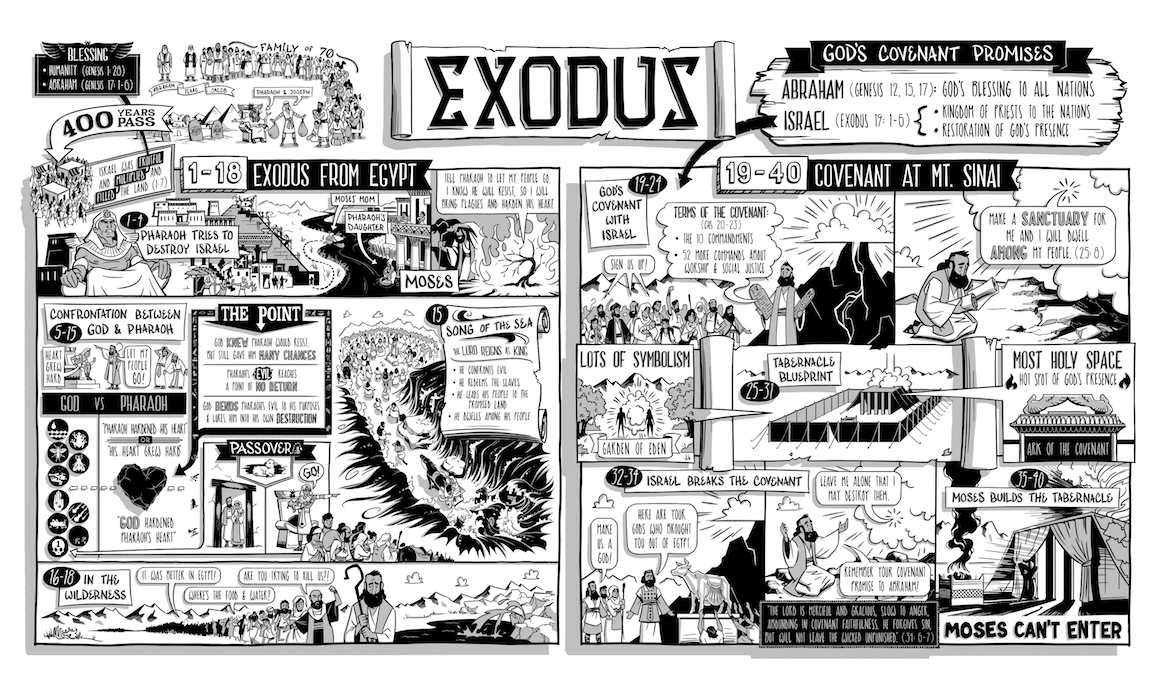
\includegraphics[scale=0.5, angle=90]{02OT-Exodus/References/BibleProject-Exodus.png}
\caption[Exodus from the Bible Project]{Exodus from the Bible Project}
\label{fig:Exodus from the Bible Project}
\end{center}
\end{figure}

\newpage
\begin{figure}
\begin{center}
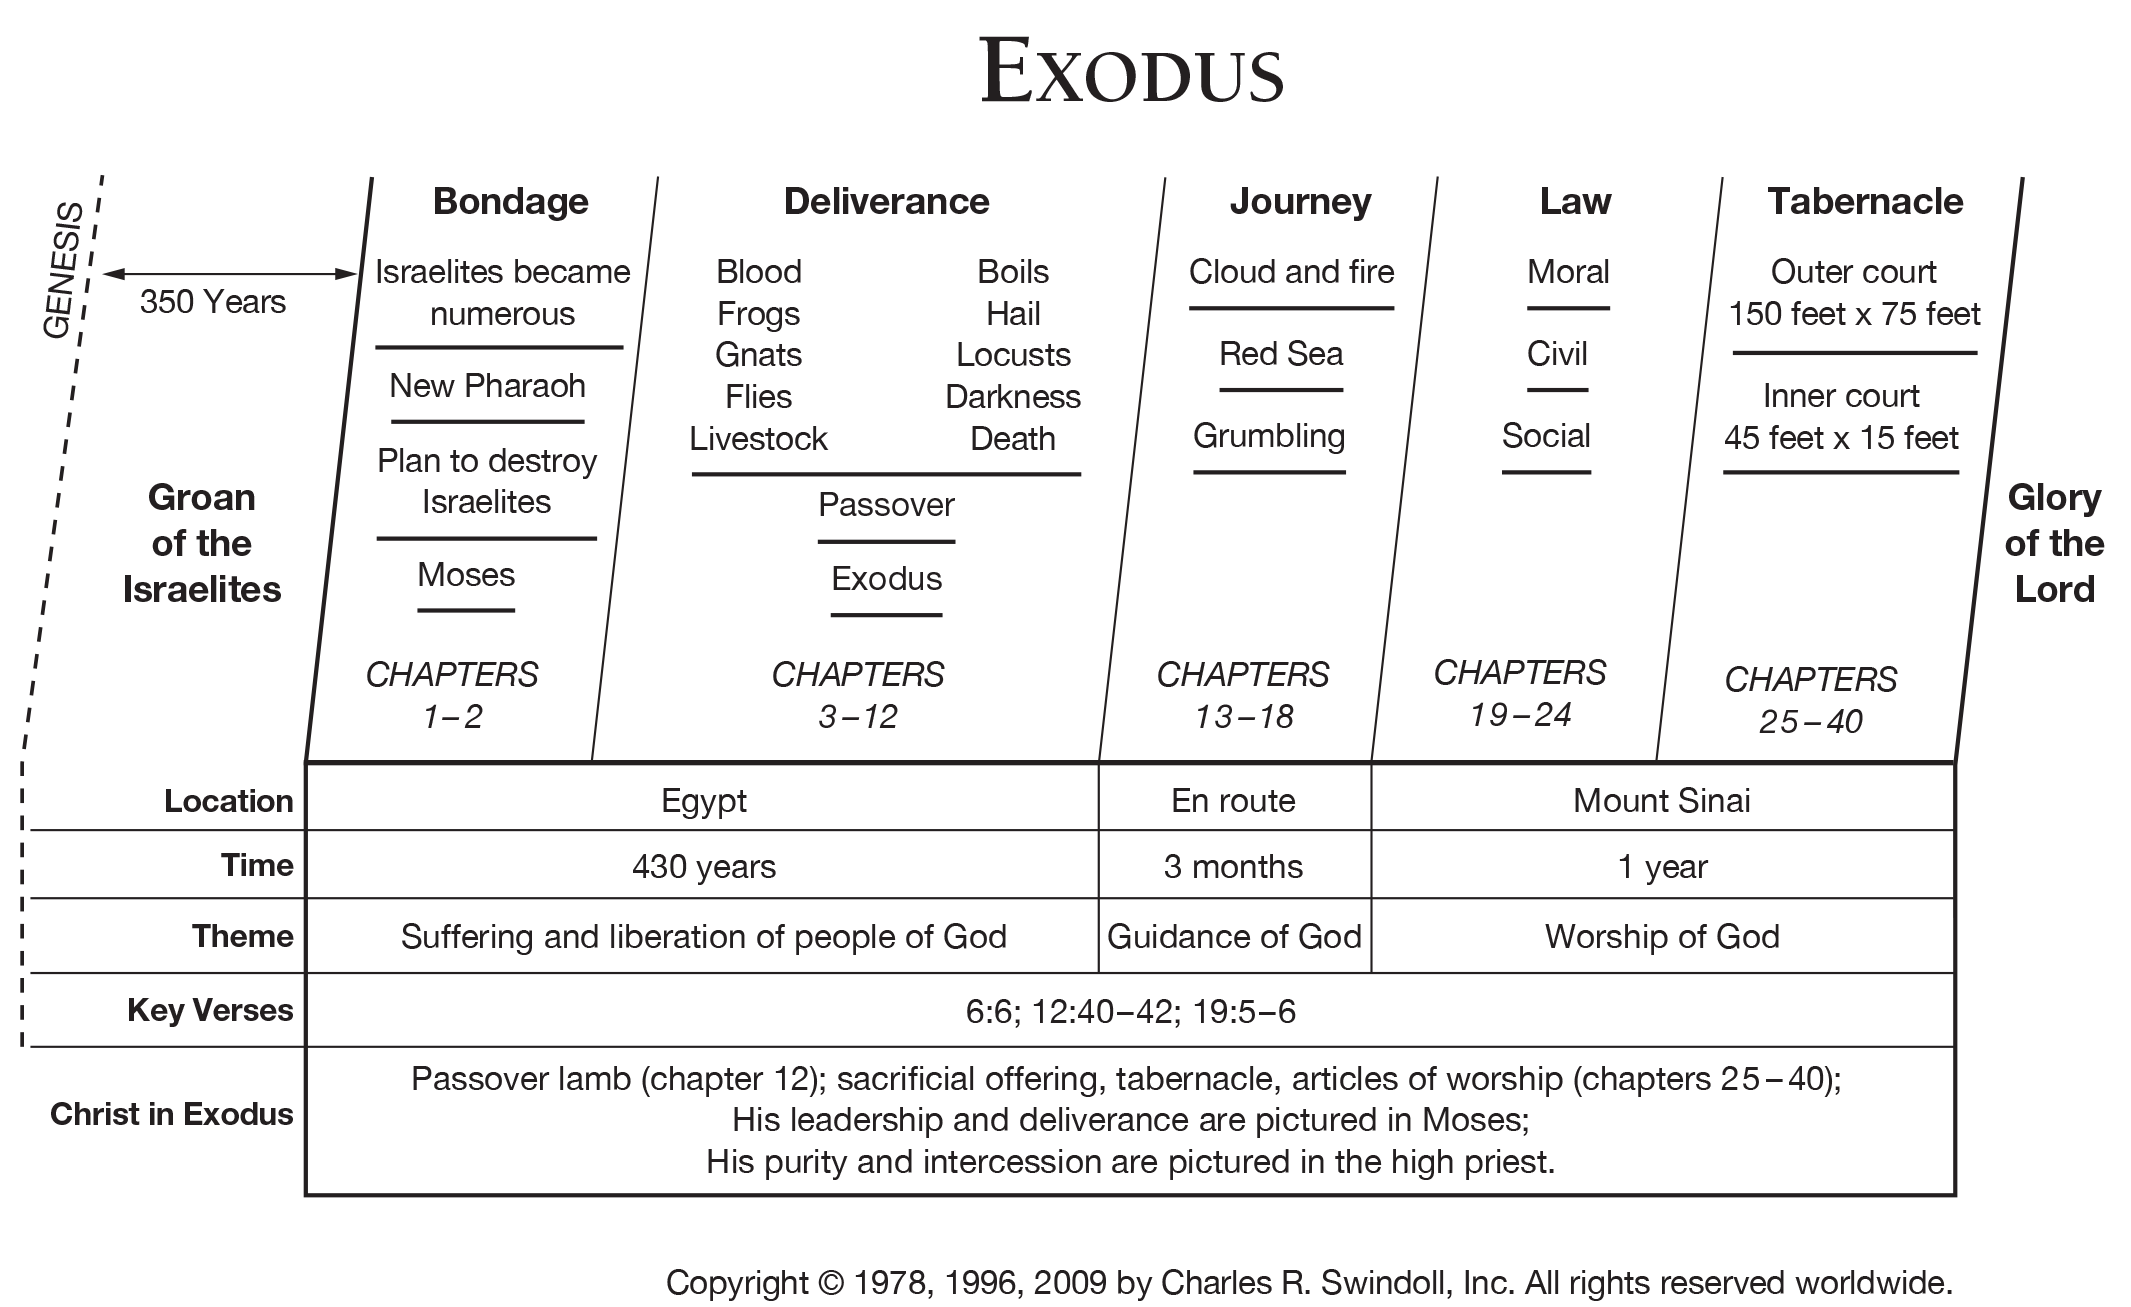
\includegraphics[scale=0.3, angle=90]{02OT-Exodus/References/Swindoll-Exodus.png}
\caption[Exodus by Swindoll]{Genesis by Exodus}
\label{fig:Exodus by Swindoll}
\end{center}
\end{figure}

\newpage
\begin{figure}
\begin{center}
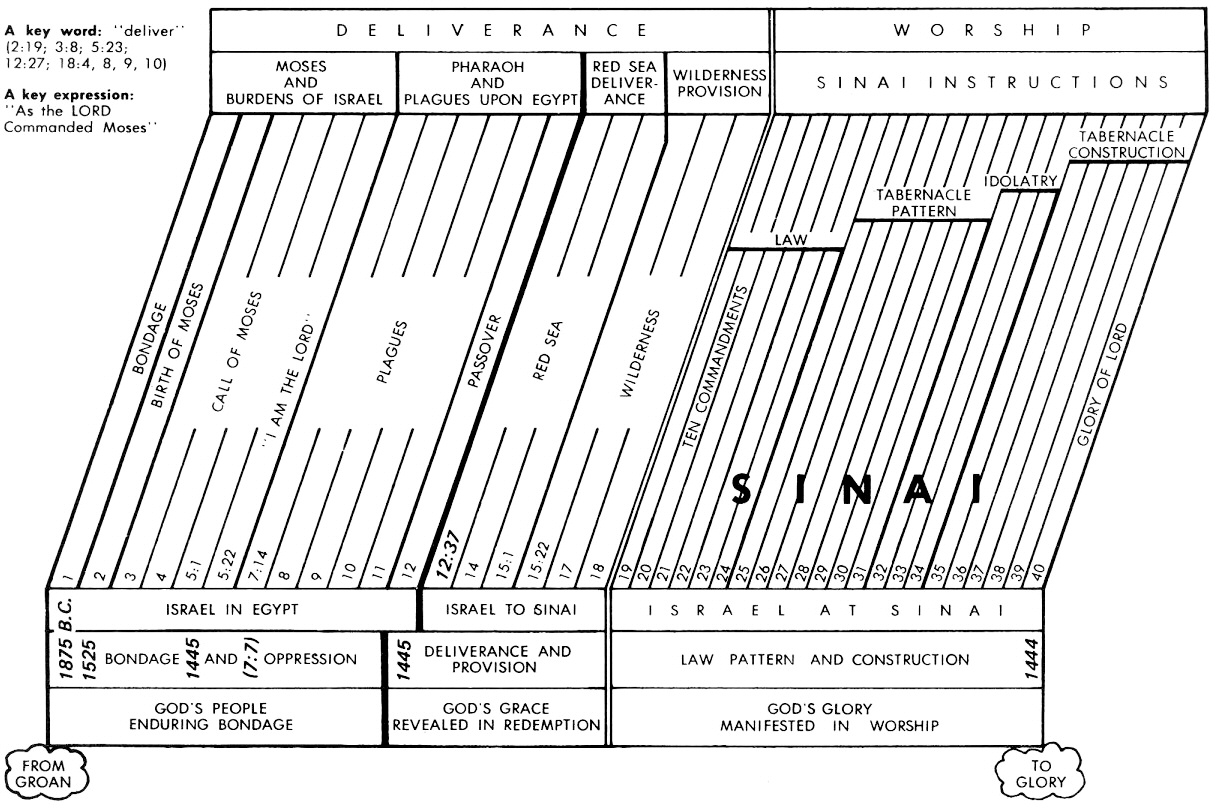
\includegraphics[scale=1.7, angle=90]{02OT-Exodus/References/Jensen-Exodus.png}
\caption[Exodus by Jensen]{Exodus by Jensen}
\label{fig:Exodus by Jensen}
\end{center}
\end{figure}

\newpage
\begin{figure}
\begin{center}
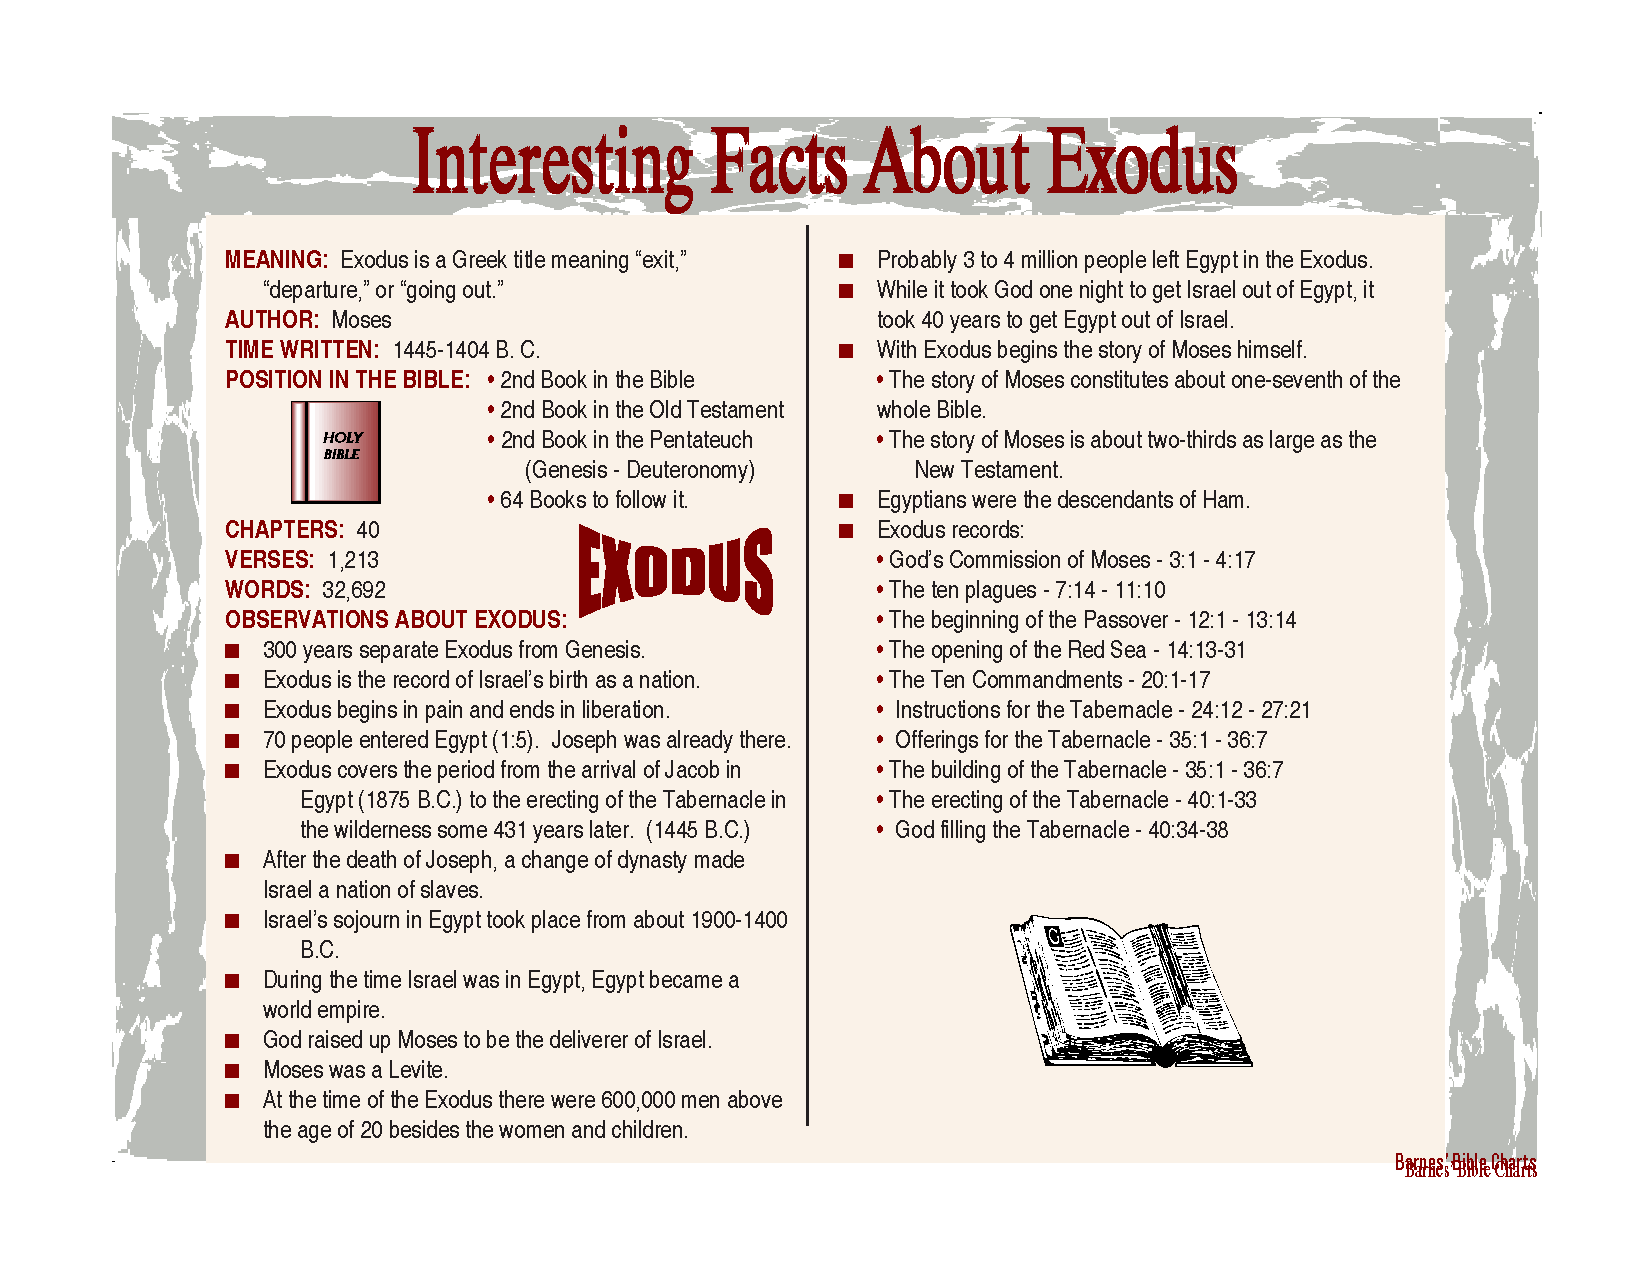
\includegraphics[scale=0.6, angle=90]{02OT-Exodus/References/interestingfactsaboutexodus.pdf}
\caption[Interesting Facts About Exodus]{Interesting Facts About Exodus}
\label{fig:Interesting Facts About Exodus}
\end{center}
\end{figure}




\chapter{Exodus 34}

\begin{figure}
  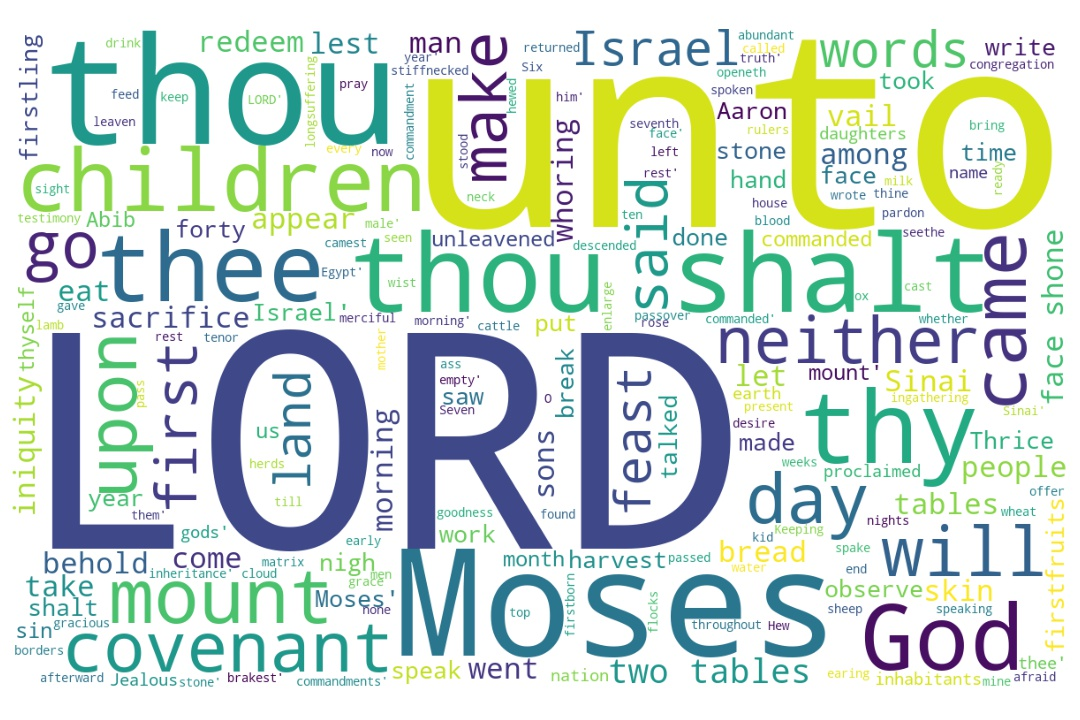
\includegraphics[width=\linewidth]{02OT-Exodus/Exodus34-WordCloud.jpg}
  \caption{Exodus 34 Word Cloud}
  \label{fig:Exodus 34 word Cloud}
\end{figure}



\marginpar{\scriptsize \centering \fcolorbox{bone}{lime}{\textbf{BE READY}}\\ (Exodus 34:1-35) \begin{compactenum}[I.][8]
    \item To \textbf{Receive Instruction} from God \index[scripture]{Exodus!Exo 34:02}(Exodus 34:2)
    \item To be \textbf{Visited} by God\index[scripture]{Exodus!Exo  19:11}(Exo 19:11)
    \item To be \textbf{Rescued} by God \index[scripture]{Esther!Est 08:13}(Est 8:13)
    \item For a \textbf{Revelation} \index[scripture]{Job!Job 18:12}(Job 18:12)
    \item To \textbf{Reject} False gods \index[scripture]{Daniel!Dan 03:15}(Dan 3:15)
    \item To \textbf{Render} Gifts \index[scripture]{2 Corinthians!2Cor 09:03}\index[scripture]{2 Corinthians!2 Corinthians 09:05}(2 Cor 9:3, 5)
   \item To \textbf{Respond} for God \index[scripture]{1 Peter!1Pet 03:15}(1 Pet 3:15)
%    \item A \textbf{Service} \index[scripture]{Exodus!Exodus 27:19}(Exodus 27:19)
%    \item A \textbf{Statute} \index[scripture]{Exodus!Exodus 27:21}(Exodus 27:21)
%    \item The \textbf{Sons} \index[scripture]{Exodus!Exodus 27:21}(Exodus 27:21)
\end{compactenum}}

%%%%%%%%%%%%%%%%%%%%%%%%%%%%%%%%%%%%%%
%%%%%%%%%%%%%%%%%%%%%%%%%%%%%%%%%%%%%
\footnote{\textcolor[cmyk]{0.99998,1,0,0}{\hyperlink{TOC}{Return to end of Table of Contents.}}}\footnote{\href{https://audiobible.com/bible/exodus_34.html}{\textcolor[cmyk]{0.99998,1,0,0}{Exodus 34 Audio}}}\textcolor[cmyk]{0.99998,1,0,0}{And the LORD said unto \fcolorbox{bone}{bone}{Moses}, Hew thee two tables of stone like unto the first: and I will write upon \emph{these} tables the words that were in the first tables, which thou brakest.}
[2] \textcolor[cmyk]{0.99998,1,0,0}{And \fcolorbox{bone}{lime}{be ready} in the morning, and come up in the morning unto mount Sinai, and present thyself there to me in the top of the mount.}
[3] \textcolor[cmyk]{0.99998,1,0,0}{And no man shall come up with thee, neither let any man be seen throughout all the mount; neither let the flocks nor herds feed before that mount.}\\
\\
\P \textcolor[cmyk]{0.99998,1,0,0}{And he hewed two tables of stone like unto the first; and \fcolorbox{bone}{bone}{Moses} rose up early in the morning, and went up unto mount Sinai, as the LORD had commanded him, and took in his hand the two tables of stone.}
[5] \textcolor[cmyk]{0.99998,1,0,0}{And the LORD descended in the cloud, and stood with him there, and proclaimed the name of the LORD.}
[6] \textcolor[cmyk]{0.99998,1,0,0}{And the LORD passed by before him, and proclaimed, The LORD, The LORD God, merciful and gracious, longsuffering, and abundant in goodness and truth,}
[7] \textcolor[cmyk]{0.99998,1,0,0}{Keeping mercy for thousands, forgiving iniquity and transgression and sin, and that will by no means clear \emph{the} \emph{guilty}; visiting the iniquity of the fathers upon the children, and upon the children's children, unto the third and to the fourth \emph{generation}.}
[8] \textcolor[cmyk]{0.99998,1,0,0}{And \fcolorbox{bone}{bone}{Moses} made haste, and bowed his head toward the earth, and worshipped.}
[9] \textcolor[cmyk]{0.99998,1,0,0}{And he said, If now I have found grace in thy sight, O Lord, let my Lord, I pray thee, go among us; for it \emph{is} a stiffnecked people; and pardon our iniquity and our sin, and take us for thine inheritance.}
[10] \textcolor[cmyk]{0.99998,1,0,0}{And he said, Behold, I make a covenant: before all thy people I will do marvels, such as have not been done in all the earth, nor in any nation: and all the people among which thou \emph{art} shall see the work of the LORD: for it \emph{is} a terrible thing that I will do with thee.}
[11] \textcolor[cmyk]{0.99998,1,0,0}{Observe thou that which I command thee \fcolorbox{bone}{lime}{this day}: behold, I drive out before thee the Amorite, and the Canaanite, and the Hittite, and the Perizzite, and the Hivite, and the Jebusite.}
[12] \textcolor[cmyk]{0.99998,1,0,0}{Take heed to thyself, lest thou make a covenant with the inhabitants of the land whither thou goest, lest it be for a snare in the midst of thee:}
[13] \textcolor[cmyk]{0.99998,1,0,0}{But ye shall destroy their altars, break their images, and cut down their groves:}
[14] \textcolor[cmyk]{0.99998,1,0,0}{For thou shalt worship no other god: for the LORD, whose name \emph{is} Jealous, \emph{is} a jealous God:}
[15] \textcolor[cmyk]{0.99998,1,0,0}{Lest thou make a covenant with the inhabitants of the land, and they go a whoring after their gods, and do sacrifice unto their gods, and \emph{one} call thee, and thou eat of his sacrifice;}
[16] \textcolor[cmyk]{0.99998,1,0,0}{And thou take of their daughters unto thy sons, and their daughters go a whoring after their gods, and make thy sons go a whoring after their gods.}
[17] \textcolor[cmyk]{0.99998,1,0,0}{Thou shalt make thee no molten gods.}\\
\\
\P \textcolor[cmyk]{0.99998,1,0,0}{The feast of unleavened bread shalt thou keep. Seven days thou shalt eat unleavened bread, as I commanded thee, in the time of the month Abib: for in the month Abib thou camest out from Egypt.}
[19] \textcolor[cmyk]{0.99998,1,0,0}{All that openeth the matrix \emph{is} mine; and every firstling among thy cattle, \emph{whether} ox or sheep, \emph{that} \emph{is} \emph{male}.}
[20] \textcolor[cmyk]{0.99998,1,0,0}{But the firstling of an ass thou shalt redeem with a lamb: and if thou redeem \emph{him} not, then shalt thou break his neck. All the firstborn of thy sons thou shalt redeem. And none shall appear before me empty.}\\
\\
\P \textcolor[cmyk]{0.99998,1,0,0}{Six days thou shalt work, but on the seventh day thou shalt rest: in earing time and in harvest thou shalt rest.}\\
\\
\P \textcolor[cmyk]{0.99998,1,0,0}{And thou shalt observe the feast of weeks, of the firstfruits of wheat harvest, and the feast of ingathering at the year's end.}\\
\\
\P \textcolor[cmyk]{0.99998,1,0,0}{Thrice in the year shall all your men children appear before the Lord GOD, the God of Israel.}
[24] \textcolor[cmyk]{0.99998,1,0,0}{For I will cast out the nations before thee, and enlarge thy borders: neither shall any man desire thy land, when thou shalt go up to appear before the LORD thy God thrice in the year.}
[25] \textcolor[cmyk]{0.99998,1,0,0}{Thou shalt not offer the blood of my sacrifice with leaven; neither shall the sacrifice of the feast of the passover be left unto the morning.}
[26] \textcolor[cmyk]{0.99998,1,0,0}{The first of the firstfruits of thy land thou shalt bring unto the house of the LORD thy God. Thou shalt not seethe a kid in his mother's milk.}
[27] \textcolor[cmyk]{0.99998,1,0,0}{And the LORD said unto \fcolorbox{bone}{bone}{Moses}, Write thou these words: for after the tenor of these words I have made a covenant with thee and with Israel.}
[28] \textcolor[cmyk]{0.99998,1,0,0}{And he was there with the LORD forty days and forty nights; he did neither eat bread, nor drink water. And he wrote upon the tables the words of the covenant, the ten commandments.}\\
\\
\P \textcolor[cmyk]{0.99998,1,0,0}{And it came to pass, when \fcolorbox{bone}{bone}{Moses} came down from mount Sinai with the two tables of testimony in Moses' hand, when he came down from the mount, that \fcolorbox{bone}{bone}{Moses} wist not that the skin of his face shone while he talked with him.}
[30] \textcolor[cmyk]{0.99998,1,0,0}{And when Aaron and all the children of Israel saw \fcolorbox{bone}{bone}{Moses}, behold, the skin of his face shone; and they were afraid to come nigh him.}
[31] \textcolor[cmyk]{0.99998,1,0,0}{And \fcolorbox{bone}{bone}{Moses} called unto them; and Aaron and all the rulers of the congregation returned unto him: and \fcolorbox{bone}{bone}{Moses} talked with them.}
[32] \textcolor[cmyk]{0.99998,1,0,0}{And afterward all the children of Israel came nigh: and he gave them in commandment all that the LORD had spoken with him in mount Sinai.}
[33] \textcolor[cmyk]{0.99998,1,0,0}{And \emph{till} \fcolorbox{bone}{bone}{Moses} had done speaking with them, he put a vail on his face.}
[34] \textcolor[cmyk]{0.99998,1,0,0}{But when \fcolorbox{bone}{bone}{Moses} went in before the LORD to speak with him, he took the vail off, until he came out. And he came out, and spake unto the children of Israel \emph{that} which he was commanded.}
[35] \textcolor[cmyk]{0.99998,1,0,0}{And the children of Israel saw the face of \fcolorbox{bone}{bone}{Moses}, that the skin of Moses' face shone: and \fcolorbox{bone}{bone}{Moses} put the vail upon his face again, until he went in to speak with him.}
\index[NWIV]{34!Exodus!Exo 34:1}\index[AWIP]{And!Exodus!Exo 34:1}\index[AWIP]{the!Exodus!Exo 34:1}\index[AWIP]{the!Exodus!Exo 34:1 (2)}\index[AWIP]{the!Exodus!Exo 34:1 (3)}\index[AWIP]{the!Exodus!Exo 34:1 (4)}\index[AWIP]{LORD!Exodus!Exo 34:1}\index[AWIP]{said!Exodus!Exo 34:1}\index[AWIP]{unto!Exodus!Exo 34:1}\index[AWIP]{unto!Exodus!Exo 34:1 (2)}\index[AWIP]{Moses!Exodus!Exo 34:1}\index[AWIP]{Hew!Exodus!Exo 34:1}\index[AWIP]{thee!Exodus!Exo 34:1}\index[AWIP]{two!Exodus!Exo 34:1}\index[AWIP]{tables!Exodus!Exo 34:1}\index[AWIP]{tables!Exodus!Exo 34:1 (2)}\index[AWIP]{tables!Exodus!Exo 34:1 (3)}\index[AWIP]{of!Exodus!Exo 34:1}\index[AWIP]{stone!Exodus!Exo 34:1}\index[AWIP]{like!Exodus!Exo 34:1}\index[AWIP]{first!Exodus!Exo 34:1}\index[AWIP]{first!Exodus!Exo 34:1 (2)}\index[AWIP]{and!Exodus!Exo 34:1}\index[AWIP]{I!Exodus!Exo 34:1}\index[AWIP]{will!Exodus!Exo 34:1}\index[AWIP]{write!Exodus!Exo 34:1}\index[AWIP]{upon!Exodus!Exo 34:1}\index[AWIP]{\emph{these}!Exodus!Exo 34:1}\index[AWIP]{words!Exodus!Exo 34:1}\index[AWIP]{that!Exodus!Exo 34:1}\index[AWIP]{were!Exodus!Exo 34:1}\index[AWIP]{in!Exodus!Exo 34:1}\index[AWIP]{which!Exodus!Exo 34:1}\index[AWIP]{thou!Exodus!Exo 34:1}\index[AWIP]{brakest!Exodus!Exo 34:1}\index[AWIP]{\emph{these}!Exodus!Exo 34:1}

\index[NWIV]{27!Exodus!Exo 34:2}\index[AWIP]{And!Exodus!Exo 34:2}\index[AWIP]{be!Exodus!Exo 34:2}\index[AWIP]{ready!Exodus!Exo 34:2}\index[AWIP]{in!Exodus!Exo 34:2}\index[AWIP]{in!Exodus!Exo 34:2 (2)}\index[AWIP]{in!Exodus!Exo 34:2 (3)}\index[AWIP]{the!Exodus!Exo 34:2}\index[AWIP]{the!Exodus!Exo 34:2 (2)}\index[AWIP]{the!Exodus!Exo 34:2 (3)}\index[AWIP]{the!Exodus!Exo 34:2 (4)}\index[AWIP]{morning!Exodus!Exo 34:2}\index[AWIP]{morning!Exodus!Exo 34:2 (2)}\index[AWIP]{and!Exodus!Exo 34:2}\index[AWIP]{and!Exodus!Exo 34:2 (2)}\index[AWIP]{come!Exodus!Exo 34:2}\index[AWIP]{up!Exodus!Exo 34:2}\index[AWIP]{unto!Exodus!Exo 34:2}\index[AWIP]{mount!Exodus!Exo 34:2}\index[AWIP]{mount!Exodus!Exo 34:2 (2)}\index[AWIP]{Sinai!Exodus!Exo 34:2}\index[AWIP]{present!Exodus!Exo 34:2}\index[AWIP]{thyself!Exodus!Exo 34:2}\index[AWIP]{there!Exodus!Exo 34:2}\index[AWIP]{to!Exodus!Exo 34:2}\index[AWIP]{me!Exodus!Exo 34:2}\index[AWIP]{top!Exodus!Exo 34:2}\index[AWIP]{of!Exodus!Exo 34:2}

\index[NWIV]{28!Exodus!Exo 34:3}\index[AWIP]{And!Exodus!Exo 34:3}\index[AWIP]{no!Exodus!Exo 34:3}\index[AWIP]{man!Exodus!Exo 34:3}\index[AWIP]{man!Exodus!Exo 34:3 (2)}\index[AWIP]{shall!Exodus!Exo 34:3}\index[AWIP]{come!Exodus!Exo 34:3}\index[AWIP]{up!Exodus!Exo 34:3}\index[AWIP]{with!Exodus!Exo 34:3}\index[AWIP]{thee!Exodus!Exo 34:3}\index[AWIP]{neither!Exodus!Exo 34:3}\index[AWIP]{neither!Exodus!Exo 34:3 (2)}\index[AWIP]{let!Exodus!Exo 34:3}\index[AWIP]{let!Exodus!Exo 34:3 (2)}\index[AWIP]{any!Exodus!Exo 34:3}\index[AWIP]{be!Exodus!Exo 34:3}\index[AWIP]{seen!Exodus!Exo 34:3}\index[AWIP]{throughout!Exodus!Exo 34:3}\index[AWIP]{all!Exodus!Exo 34:3}\index[AWIP]{the!Exodus!Exo 34:3}\index[AWIP]{the!Exodus!Exo 34:3 (2)}\index[AWIP]{mount!Exodus!Exo 34:3}\index[AWIP]{mount!Exodus!Exo 34:3 (2)}\index[AWIP]{flocks!Exodus!Exo 34:3}\index[AWIP]{nor!Exodus!Exo 34:3}\index[AWIP]{herds!Exodus!Exo 34:3}\index[AWIP]{feed!Exodus!Exo 34:3}\index[AWIP]{before!Exodus!Exo 34:3}\index[AWIP]{that!Exodus!Exo 34:3}

\index[NWIV]{41!Exodus!Exo 34:4}\index[AWIP]{And!Exodus!Exo 34:4}\index[AWIP]{he!Exodus!Exo 34:4}\index[AWIP]{hewed!Exodus!Exo 34:4}\index[AWIP]{two!Exodus!Exo 34:4}\index[AWIP]{two!Exodus!Exo 34:4 (2)}\index[AWIP]{tables!Exodus!Exo 34:4}\index[AWIP]{tables!Exodus!Exo 34:4 (2)}\index[AWIP]{of!Exodus!Exo 34:4}\index[AWIP]{of!Exodus!Exo 34:4 (2)}\index[AWIP]{stone!Exodus!Exo 34:4}\index[AWIP]{stone!Exodus!Exo 34:4 (2)}\index[AWIP]{like!Exodus!Exo 34:4}\index[AWIP]{unto!Exodus!Exo 34:4}\index[AWIP]{unto!Exodus!Exo 34:4 (2)}\index[AWIP]{the!Exodus!Exo 34:4}\index[AWIP]{the!Exodus!Exo 34:4 (2)}\index[AWIP]{the!Exodus!Exo 34:4 (3)}\index[AWIP]{the!Exodus!Exo 34:4 (4)}\index[AWIP]{first!Exodus!Exo 34:4}\index[AWIP]{and!Exodus!Exo 34:4}\index[AWIP]{and!Exodus!Exo 34:4 (2)}\index[AWIP]{and!Exodus!Exo 34:4 (3)}\index[AWIP]{Moses!Exodus!Exo 34:4}\index[AWIP]{rose!Exodus!Exo 34:4}\index[AWIP]{up!Exodus!Exo 34:4}\index[AWIP]{up!Exodus!Exo 34:4 (2)}\index[AWIP]{early!Exodus!Exo 34:4}\index[AWIP]{in!Exodus!Exo 34:4}\index[AWIP]{in!Exodus!Exo 34:4 (2)}\index[AWIP]{morning!Exodus!Exo 34:4}\index[AWIP]{went!Exodus!Exo 34:4}\index[AWIP]{mount!Exodus!Exo 34:4}\index[AWIP]{Sinai!Exodus!Exo 34:4}\index[AWIP]{as!Exodus!Exo 34:4}\index[AWIP]{LORD!Exodus!Exo 34:4}\index[AWIP]{had!Exodus!Exo 34:4}\index[AWIP]{commanded!Exodus!Exo 34:4}\index[AWIP]{him!Exodus!Exo 34:4}\index[AWIP]{took!Exodus!Exo 34:4}\index[AWIP]{his!Exodus!Exo 34:4}\index[AWIP]{hand!Exodus!Exo 34:4}

\index[NWIV]{19!Exodus!Exo 34:5}\index[AWIP]{And!Exodus!Exo 34:5}\index[AWIP]{the!Exodus!Exo 34:5}\index[AWIP]{the!Exodus!Exo 34:5 (2)}\index[AWIP]{the!Exodus!Exo 34:5 (3)}\index[AWIP]{the!Exodus!Exo 34:5 (4)}\index[AWIP]{LORD!Exodus!Exo 34:5}\index[AWIP]{LORD!Exodus!Exo 34:5 (2)}\index[AWIP]{descended!Exodus!Exo 34:5}\index[AWIP]{in!Exodus!Exo 34:5}\index[AWIP]{cloud!Exodus!Exo 34:5}\index[AWIP]{and!Exodus!Exo 34:5}\index[AWIP]{and!Exodus!Exo 34:5 (2)}\index[AWIP]{stood!Exodus!Exo 34:5}\index[AWIP]{with!Exodus!Exo 34:5}\index[AWIP]{him!Exodus!Exo 34:5}\index[AWIP]{there!Exodus!Exo 34:5}\index[AWIP]{proclaimed!Exodus!Exo 34:5}\index[AWIP]{name!Exodus!Exo 34:5}\index[AWIP]{of!Exodus!Exo 34:5}

\index[NWIV]{24!Exodus!Exo 34:6}\index[AWIP]{And!Exodus!Exo 34:6}\index[AWIP]{the!Exodus!Exo 34:6}\index[AWIP]{LORD!Exodus!Exo 34:6}\index[AWIP]{LORD!Exodus!Exo 34:6 (2)}\index[AWIP]{LORD!Exodus!Exo 34:6 (3)}\index[AWIP]{passed!Exodus!Exo 34:6}\index[AWIP]{by!Exodus!Exo 34:6}\index[AWIP]{before!Exodus!Exo 34:6}\index[AWIP]{him!Exodus!Exo 34:6}\index[AWIP]{and!Exodus!Exo 34:6}\index[AWIP]{and!Exodus!Exo 34:6 (2)}\index[AWIP]{and!Exodus!Exo 34:6 (3)}\index[AWIP]{and!Exodus!Exo 34:6 (4)}\index[AWIP]{proclaimed!Exodus!Exo 34:6}\index[AWIP]{The!Exodus!Exo 34:6}\index[AWIP]{The!Exodus!Exo 34:6 (2)}\index[AWIP]{God!Exodus!Exo 34:6}\index[AWIP]{merciful!Exodus!Exo 34:6}\index[AWIP]{gracious!Exodus!Exo 34:6}\index[AWIP]{longsuffering!Exodus!Exo 34:6}\index[AWIP]{abundant!Exodus!Exo 34:6}\index[AWIP]{in!Exodus!Exo 34:6}\index[AWIP]{goodness!Exodus!Exo 34:6}\index[AWIP]{truth!Exodus!Exo 34:6}

\index[NWIV]{41!Exodus!Exo 34:7}\index[AWIP]{Keeping!Exodus!Exo 34:7}\index[AWIP]{mercy!Exodus!Exo 34:7}\index[AWIP]{for!Exodus!Exo 34:7}\index[AWIP]{thousands!Exodus!Exo 34:7}\index[AWIP]{forgiving!Exodus!Exo 34:7}\index[AWIP]{iniquity!Exodus!Exo 34:7}\index[AWIP]{iniquity!Exodus!Exo 34:7 (2)}\index[AWIP]{and!Exodus!Exo 34:7}\index[AWIP]{and!Exodus!Exo 34:7 (2)}\index[AWIP]{and!Exodus!Exo 34:7 (3)}\index[AWIP]{and!Exodus!Exo 34:7 (4)}\index[AWIP]{and!Exodus!Exo 34:7 (5)}\index[AWIP]{transgression!Exodus!Exo 34:7}\index[AWIP]{sin!Exodus!Exo 34:7}\index[AWIP]{that!Exodus!Exo 34:7}\index[AWIP]{will!Exodus!Exo 34:7}\index[AWIP]{by!Exodus!Exo 34:7}\index[AWIP]{no!Exodus!Exo 34:7}\index[AWIP]{means!Exodus!Exo 34:7}\index[AWIP]{clear!Exodus!Exo 34:7}\index[AWIP]{\emph{the}!Exodus!Exo 34:7}\index[AWIP]{\emph{guilty}!Exodus!Exo 34:7}\index[AWIP]{visiting!Exodus!Exo 34:7}\index[AWIP]{the!Exodus!Exo 34:7}\index[AWIP]{the!Exodus!Exo 34:7 (2)}\index[AWIP]{the!Exodus!Exo 34:7 (3)}\index[AWIP]{the!Exodus!Exo 34:7 (4)}\index[AWIP]{the!Exodus!Exo 34:7 (5)}\index[AWIP]{the!Exodus!Exo 34:7 (6)}\index[AWIP]{of!Exodus!Exo 34:7}\index[AWIP]{fathers!Exodus!Exo 34:7}\index[AWIP]{upon!Exodus!Exo 34:7}\index[AWIP]{upon!Exodus!Exo 34:7 (2)}\index[AWIP]{children!Exodus!Exo 34:7}\index[AWIP]{children!Exodus!Exo 34:7 (2)}\index[AWIP]{children's!Exodus!Exo 34:7}\index[AWIP]{unto!Exodus!Exo 34:7}\index[AWIP]{third!Exodus!Exo 34:7}\index[AWIP]{to!Exodus!Exo 34:7}\index[AWIP]{fourth!Exodus!Exo 34:7}\index[AWIP]{\emph{generation}!Exodus!Exo 34:7}\index[AWIP]{\emph{the}!Exodus!Exo 34:7}\index[AWIP]{\emph{guilty}!Exodus!Exo 34:7}\index[AWIP]{\emph{generation}!Exodus!Exo 34:7}

\index[NWIV]{13!Exodus!Exo 34:8}\index[AWIP]{And!Exodus!Exo 34:8}\index[AWIP]{Moses!Exodus!Exo 34:8}\index[AWIP]{made!Exodus!Exo 34:8}\index[AWIP]{haste!Exodus!Exo 34:8}\index[AWIP]{and!Exodus!Exo 34:8}\index[AWIP]{and!Exodus!Exo 34:8 (2)}\index[AWIP]{bowed!Exodus!Exo 34:8}\index[AWIP]{his!Exodus!Exo 34:8}\index[AWIP]{head!Exodus!Exo 34:8}\index[AWIP]{toward!Exodus!Exo 34:8}\index[AWIP]{the!Exodus!Exo 34:8}\index[AWIP]{earth!Exodus!Exo 34:8}\index[AWIP]{worshipped!Exodus!Exo 34:8}

\index[NWIV]{42!Exodus!Exo 34:9}\index[AWIP]{And!Exodus!Exo 34:9}\index[AWIP]{he!Exodus!Exo 34:9}\index[AWIP]{said!Exodus!Exo 34:9}\index[AWIP]{If!Exodus!Exo 34:9}\index[AWIP]{now!Exodus!Exo 34:9}\index[AWIP]{I!Exodus!Exo 34:9}\index[AWIP]{I!Exodus!Exo 34:9 (2)}\index[AWIP]{have!Exodus!Exo 34:9}\index[AWIP]{found!Exodus!Exo 34:9}\index[AWIP]{grace!Exodus!Exo 34:9}\index[AWIP]{in!Exodus!Exo 34:9}\index[AWIP]{thy!Exodus!Exo 34:9}\index[AWIP]{sight!Exodus!Exo 34:9}\index[AWIP]{O!Exodus!Exo 34:9}\index[AWIP]{Lord!Exodus!Exo 34:9}\index[AWIP]{Lord!Exodus!Exo 34:9 (2)}\index[AWIP]{let!Exodus!Exo 34:9}\index[AWIP]{my!Exodus!Exo 34:9}\index[AWIP]{pray!Exodus!Exo 34:9}\index[AWIP]{thee!Exodus!Exo 34:9}\index[AWIP]{go!Exodus!Exo 34:9}\index[AWIP]{among!Exodus!Exo 34:9}\index[AWIP]{us!Exodus!Exo 34:9}\index[AWIP]{us!Exodus!Exo 34:9 (2)}\index[AWIP]{for!Exodus!Exo 34:9}\index[AWIP]{for!Exodus!Exo 34:9 (2)}\index[AWIP]{it!Exodus!Exo 34:9}\index[AWIP]{\emph{is}!Exodus!Exo 34:9}\index[AWIP]{a!Exodus!Exo 34:9}\index[AWIP]{stiffnecked!Exodus!Exo 34:9}\index[AWIP]{people!Exodus!Exo 34:9}\index[AWIP]{and!Exodus!Exo 34:9}\index[AWIP]{and!Exodus!Exo 34:9 (2)}\index[AWIP]{and!Exodus!Exo 34:9 (3)}\index[AWIP]{pardon!Exodus!Exo 34:9}\index[AWIP]{our!Exodus!Exo 34:9}\index[AWIP]{our!Exodus!Exo 34:9 (2)}\index[AWIP]{iniquity!Exodus!Exo 34:9}\index[AWIP]{sin!Exodus!Exo 34:9}\index[AWIP]{take!Exodus!Exo 34:9}\index[AWIP]{thine!Exodus!Exo 34:9}\index[AWIP]{inheritance!Exodus!Exo 34:9}\index[AWIP]{\emph{is}!Exodus!Exo 34:9}

\index[NWIV]{57!Exodus!Exo 34:10}\index[AWIP]{And!Exodus!Exo 34:10}\index[AWIP]{he!Exodus!Exo 34:10}\index[AWIP]{said!Exodus!Exo 34:10}\index[AWIP]{Behold!Exodus!Exo 34:10}\index[AWIP]{I!Exodus!Exo 34:10}\index[AWIP]{I!Exodus!Exo 34:10 (2)}\index[AWIP]{I!Exodus!Exo 34:10 (3)}\index[AWIP]{make!Exodus!Exo 34:10}\index[AWIP]{a!Exodus!Exo 34:10}\index[AWIP]{a!Exodus!Exo 34:10 (2)}\index[AWIP]{covenant!Exodus!Exo 34:10}\index[AWIP]{before!Exodus!Exo 34:10}\index[AWIP]{all!Exodus!Exo 34:10}\index[AWIP]{all!Exodus!Exo 34:10 (2)}\index[AWIP]{all!Exodus!Exo 34:10 (3)}\index[AWIP]{thy!Exodus!Exo 34:10}\index[AWIP]{people!Exodus!Exo 34:10}\index[AWIP]{people!Exodus!Exo 34:10 (2)}\index[AWIP]{will!Exodus!Exo 34:10}\index[AWIP]{will!Exodus!Exo 34:10 (2)}\index[AWIP]{do!Exodus!Exo 34:10}\index[AWIP]{do!Exodus!Exo 34:10 (2)}\index[AWIP]{marvels!Exodus!Exo 34:10}\index[AWIP]{such!Exodus!Exo 34:10}\index[AWIP]{as!Exodus!Exo 34:10}\index[AWIP]{have!Exodus!Exo 34:10}\index[AWIP]{not!Exodus!Exo 34:10}\index[AWIP]{been!Exodus!Exo 34:10}\index[AWIP]{done!Exodus!Exo 34:10}\index[AWIP]{in!Exodus!Exo 34:10}\index[AWIP]{in!Exodus!Exo 34:10 (2)}\index[AWIP]{the!Exodus!Exo 34:10}\index[AWIP]{the!Exodus!Exo 34:10 (2)}\index[AWIP]{the!Exodus!Exo 34:10 (3)}\index[AWIP]{the!Exodus!Exo 34:10 (4)}\index[AWIP]{earth!Exodus!Exo 34:10}\index[AWIP]{nor!Exodus!Exo 34:10}\index[AWIP]{any!Exodus!Exo 34:10}\index[AWIP]{nation!Exodus!Exo 34:10}\index[AWIP]{and!Exodus!Exo 34:10}\index[AWIP]{among!Exodus!Exo 34:10}\index[AWIP]{which!Exodus!Exo 34:10}\index[AWIP]{thou!Exodus!Exo 34:10}\index[AWIP]{\emph{art}!Exodus!Exo 34:10}\index[AWIP]{shall!Exodus!Exo 34:10}\index[AWIP]{see!Exodus!Exo 34:10}\index[AWIP]{work!Exodus!Exo 34:10}\index[AWIP]{of!Exodus!Exo 34:10}\index[AWIP]{LORD!Exodus!Exo 34:10}\index[AWIP]{for!Exodus!Exo 34:10}\index[AWIP]{it!Exodus!Exo 34:10}\index[AWIP]{\emph{is}!Exodus!Exo 34:10}\index[AWIP]{terrible!Exodus!Exo 34:10}\index[AWIP]{thing!Exodus!Exo 34:10}\index[AWIP]{that!Exodus!Exo 34:10}\index[AWIP]{with!Exodus!Exo 34:10}\index[AWIP]{thee!Exodus!Exo 34:10}\index[AWIP]{\emph{art}!Exodus!Exo 34:10}\index[AWIP]{\emph{is}!Exodus!Exo 34:10}

\index[NWIV]{32!Exodus!Exo 34:11}\index[AWIP]{Observe!Exodus!Exo 34:11}\index[AWIP]{thou!Exodus!Exo 34:11}\index[AWIP]{that!Exodus!Exo 34:11}\index[AWIP]{which!Exodus!Exo 34:11}\index[AWIP]{I!Exodus!Exo 34:11}\index[AWIP]{I!Exodus!Exo 34:11 (2)}\index[AWIP]{command!Exodus!Exo 34:11}\index[AWIP]{thee!Exodus!Exo 34:11}\index[AWIP]{thee!Exodus!Exo 34:11 (2)}\index[AWIP]{this!Exodus!Exo 34:11}\index[AWIP]{day!Exodus!Exo 34:11}\index[AWIP]{behold!Exodus!Exo 34:11}\index[AWIP]{drive!Exodus!Exo 34:11}\index[AWIP]{out!Exodus!Exo 34:11}\index[AWIP]{before!Exodus!Exo 34:11}\index[AWIP]{the!Exodus!Exo 34:11}\index[AWIP]{the!Exodus!Exo 34:11 (2)}\index[AWIP]{the!Exodus!Exo 34:11 (3)}\index[AWIP]{the!Exodus!Exo 34:11 (4)}\index[AWIP]{the!Exodus!Exo 34:11 (5)}\index[AWIP]{the!Exodus!Exo 34:11 (6)}\index[AWIP]{Amorite!Exodus!Exo 34:11}\index[AWIP]{and!Exodus!Exo 34:11}\index[AWIP]{and!Exodus!Exo 34:11 (2)}\index[AWIP]{and!Exodus!Exo 34:11 (3)}\index[AWIP]{and!Exodus!Exo 34:11 (4)}\index[AWIP]{and!Exodus!Exo 34:11 (5)}\index[AWIP]{Canaanite!Exodus!Exo 34:11}\index[AWIP]{Hittite!Exodus!Exo 34:11}\index[AWIP]{Perizzite!Exodus!Exo 34:11}\index[AWIP]{Hivite!Exodus!Exo 34:11}\index[AWIP]{Jebusite!Exodus!Exo 34:11}

\index[NWIV]{29!Exodus!Exo 34:12}\index[AWIP]{Take!Exodus!Exo 34:12}\index[AWIP]{heed!Exodus!Exo 34:12}\index[AWIP]{to!Exodus!Exo 34:12}\index[AWIP]{thyself!Exodus!Exo 34:12}\index[AWIP]{lest!Exodus!Exo 34:12}\index[AWIP]{lest!Exodus!Exo 34:12 (2)}\index[AWIP]{thou!Exodus!Exo 34:12}\index[AWIP]{thou!Exodus!Exo 34:12 (2)}\index[AWIP]{make!Exodus!Exo 34:12}\index[AWIP]{a!Exodus!Exo 34:12}\index[AWIP]{a!Exodus!Exo 34:12 (2)}\index[AWIP]{covenant!Exodus!Exo 34:12}\index[AWIP]{with!Exodus!Exo 34:12}\index[AWIP]{the!Exodus!Exo 34:12}\index[AWIP]{the!Exodus!Exo 34:12 (2)}\index[AWIP]{the!Exodus!Exo 34:12 (3)}\index[AWIP]{inhabitants!Exodus!Exo 34:12}\index[AWIP]{of!Exodus!Exo 34:12}\index[AWIP]{of!Exodus!Exo 34:12 (2)}\index[AWIP]{land!Exodus!Exo 34:12}\index[AWIP]{whither!Exodus!Exo 34:12}\index[AWIP]{goest!Exodus!Exo 34:12}\index[AWIP]{it!Exodus!Exo 34:12}\index[AWIP]{be!Exodus!Exo 34:12}\index[AWIP]{for!Exodus!Exo 34:12}\index[AWIP]{snare!Exodus!Exo 34:12}\index[AWIP]{in!Exodus!Exo 34:12}\index[AWIP]{midst!Exodus!Exo 34:12}\index[AWIP]{thee!Exodus!Exo 34:12}

\index[NWIV]{14!Exodus!Exo 34:13}\index[AWIP]{But!Exodus!Exo 34:13}\index[AWIP]{ye!Exodus!Exo 34:13}\index[AWIP]{shall!Exodus!Exo 34:13}\index[AWIP]{destroy!Exodus!Exo 34:13}\index[AWIP]{their!Exodus!Exo 34:13}\index[AWIP]{their!Exodus!Exo 34:13 (2)}\index[AWIP]{their!Exodus!Exo 34:13 (3)}\index[AWIP]{altars!Exodus!Exo 34:13}\index[AWIP]{break!Exodus!Exo 34:13}\index[AWIP]{images!Exodus!Exo 34:13}\index[AWIP]{and!Exodus!Exo 34:13}\index[AWIP]{cut!Exodus!Exo 34:13}\index[AWIP]{down!Exodus!Exo 34:13}\index[AWIP]{groves!Exodus!Exo 34:13}

\index[NWIV]{18!Exodus!Exo 34:14}\index[AWIP]{For!Exodus!Exo 34:14}\index[AWIP]{thou!Exodus!Exo 34:14}\index[AWIP]{shalt!Exodus!Exo 34:14}\index[AWIP]{worship!Exodus!Exo 34:14}\index[AWIP]{no!Exodus!Exo 34:14}\index[AWIP]{other!Exodus!Exo 34:14}\index[AWIP]{god!Exodus!Exo 34:14}\index[AWIP]{for!Exodus!Exo 34:14}\index[AWIP]{the!Exodus!Exo 34:14}\index[AWIP]{LORD!Exodus!Exo 34:14}\index[AWIP]{whose!Exodus!Exo 34:14}\index[AWIP]{name!Exodus!Exo 34:14}\index[AWIP]{\emph{is}!Exodus!Exo 34:14}\index[AWIP]{\emph{is}!Exodus!Exo 34:14 (2)}\index[AWIP]{Jealous!Exodus!Exo 34:14}\index[AWIP]{a!Exodus!Exo 34:14}\index[AWIP]{jealous!Exodus!Exo 34:14}\index[AWIP]{God!Exodus!Exo 34:14}\index[AWIP]{\emph{is}!Exodus!Exo 34:14}\index[AWIP]{\emph{is}!Exodus!Exo 34:14 (2)}

\index[NWIV]{35!Exodus!Exo 34:15}\index[AWIP]{Lest!Exodus!Exo 34:15}\index[AWIP]{thou!Exodus!Exo 34:15}\index[AWIP]{thou!Exodus!Exo 34:15 (2)}\index[AWIP]{make!Exodus!Exo 34:15}\index[AWIP]{a!Exodus!Exo 34:15}\index[AWIP]{a!Exodus!Exo 34:15 (2)}\index[AWIP]{covenant!Exodus!Exo 34:15}\index[AWIP]{with!Exodus!Exo 34:15}\index[AWIP]{the!Exodus!Exo 34:15}\index[AWIP]{the!Exodus!Exo 34:15 (2)}\index[AWIP]{inhabitants!Exodus!Exo 34:15}\index[AWIP]{of!Exodus!Exo 34:15}\index[AWIP]{of!Exodus!Exo 34:15 (2)}\index[AWIP]{land!Exodus!Exo 34:15}\index[AWIP]{and!Exodus!Exo 34:15}\index[AWIP]{and!Exodus!Exo 34:15 (2)}\index[AWIP]{and!Exodus!Exo 34:15 (3)}\index[AWIP]{and!Exodus!Exo 34:15 (4)}\index[AWIP]{they!Exodus!Exo 34:15}\index[AWIP]{go!Exodus!Exo 34:15}\index[AWIP]{whoring!Exodus!Exo 34:15}\index[AWIP]{after!Exodus!Exo 34:15}\index[AWIP]{their!Exodus!Exo 34:15}\index[AWIP]{their!Exodus!Exo 34:15 (2)}\index[AWIP]{gods!Exodus!Exo 34:15}\index[AWIP]{gods!Exodus!Exo 34:15 (2)}\index[AWIP]{do!Exodus!Exo 34:15}\index[AWIP]{sacrifice!Exodus!Exo 34:15}\index[AWIP]{sacrifice!Exodus!Exo 34:15 (2)}\index[AWIP]{unto!Exodus!Exo 34:15}\index[AWIP]{\emph{one}!Exodus!Exo 34:15}\index[AWIP]{call!Exodus!Exo 34:15}\index[AWIP]{thee!Exodus!Exo 34:15}\index[AWIP]{eat!Exodus!Exo 34:15}\index[AWIP]{his!Exodus!Exo 34:15}\index[AWIP]{\emph{one}!Exodus!Exo 34:15}

\index[NWIV]{28!Exodus!Exo 34:16}\index[AWIP]{And!Exodus!Exo 34:16}\index[AWIP]{thou!Exodus!Exo 34:16}\index[AWIP]{take!Exodus!Exo 34:16}\index[AWIP]{of!Exodus!Exo 34:16}\index[AWIP]{their!Exodus!Exo 34:16}\index[AWIP]{their!Exodus!Exo 34:16 (2)}\index[AWIP]{their!Exodus!Exo 34:16 (3)}\index[AWIP]{their!Exodus!Exo 34:16 (4)}\index[AWIP]{daughters!Exodus!Exo 34:16}\index[AWIP]{daughters!Exodus!Exo 34:16 (2)}\index[AWIP]{unto!Exodus!Exo 34:16}\index[AWIP]{thy!Exodus!Exo 34:16}\index[AWIP]{thy!Exodus!Exo 34:16 (2)}\index[AWIP]{sons!Exodus!Exo 34:16}\index[AWIP]{sons!Exodus!Exo 34:16 (2)}\index[AWIP]{and!Exodus!Exo 34:16}\index[AWIP]{and!Exodus!Exo 34:16 (2)}\index[AWIP]{go!Exodus!Exo 34:16}\index[AWIP]{go!Exodus!Exo 34:16 (2)}\index[AWIP]{a!Exodus!Exo 34:16}\index[AWIP]{a!Exodus!Exo 34:16 (2)}\index[AWIP]{whoring!Exodus!Exo 34:16}\index[AWIP]{whoring!Exodus!Exo 34:16 (2)}\index[AWIP]{after!Exodus!Exo 34:16}\index[AWIP]{after!Exodus!Exo 34:16 (2)}\index[AWIP]{gods!Exodus!Exo 34:16}\index[AWIP]{gods!Exodus!Exo 34:16 (2)}\index[AWIP]{make!Exodus!Exo 34:16}

\index[NWIV]{7!Exodus!Exo 34:17}\index[AWIP]{Thou!Exodus!Exo 34:17}\index[AWIP]{shalt!Exodus!Exo 34:17}\index[AWIP]{make!Exodus!Exo 34:17}\index[AWIP]{thee!Exodus!Exo 34:17}\index[AWIP]{no!Exodus!Exo 34:17}\index[AWIP]{molten!Exodus!Exo 34:17}\index[AWIP]{gods!Exodus!Exo 34:17}

\index[NWIV]{36!Exodus!Exo 34:18}\index[AWIP]{The!Exodus!Exo 34:18}\index[AWIP]{feast!Exodus!Exo 34:18}\index[AWIP]{of!Exodus!Exo 34:18}\index[AWIP]{of!Exodus!Exo 34:18 (2)}\index[AWIP]{unleavened!Exodus!Exo 34:18}\index[AWIP]{unleavened!Exodus!Exo 34:18 (2)}\index[AWIP]{bread!Exodus!Exo 34:18}\index[AWIP]{bread!Exodus!Exo 34:18 (2)}\index[AWIP]{shalt!Exodus!Exo 34:18}\index[AWIP]{shalt!Exodus!Exo 34:18 (2)}\index[AWIP]{thou!Exodus!Exo 34:18}\index[AWIP]{thou!Exodus!Exo 34:18 (2)}\index[AWIP]{thou!Exodus!Exo 34:18 (3)}\index[AWIP]{keep!Exodus!Exo 34:18}\index[AWIP]{Seven!Exodus!Exo 34:18}\index[AWIP]{days!Exodus!Exo 34:18}\index[AWIP]{eat!Exodus!Exo 34:18}\index[AWIP]{as!Exodus!Exo 34:18}\index[AWIP]{I!Exodus!Exo 34:18}\index[AWIP]{commanded!Exodus!Exo 34:18}\index[AWIP]{thee!Exodus!Exo 34:18}\index[AWIP]{in!Exodus!Exo 34:18}\index[AWIP]{in!Exodus!Exo 34:18 (2)}\index[AWIP]{the!Exodus!Exo 34:18}\index[AWIP]{the!Exodus!Exo 34:18 (2)}\index[AWIP]{the!Exodus!Exo 34:18 (3)}\index[AWIP]{time!Exodus!Exo 34:18}\index[AWIP]{month!Exodus!Exo 34:18}\index[AWIP]{month!Exodus!Exo 34:18 (2)}\index[AWIP]{Abib!Exodus!Exo 34:18}\index[AWIP]{Abib!Exodus!Exo 34:18 (2)}\index[AWIP]{for!Exodus!Exo 34:18}\index[AWIP]{camest!Exodus!Exo 34:18}\index[AWIP]{out!Exodus!Exo 34:18}\index[AWIP]{from!Exodus!Exo 34:18}\index[AWIP]{Egypt!Exodus!Exo 34:18}

\index[NWIV]{20!Exodus!Exo 34:19}\index[AWIP]{All!Exodus!Exo 34:19}\index[AWIP]{that!Exodus!Exo 34:19}\index[AWIP]{openeth!Exodus!Exo 34:19}\index[AWIP]{the!Exodus!Exo 34:19}\index[AWIP]{matrix!Exodus!Exo 34:19}\index[AWIP]{\emph{is}!Exodus!Exo 34:19}\index[AWIP]{\emph{is}!Exodus!Exo 34:19 (2)}\index[AWIP]{mine!Exodus!Exo 34:19}\index[AWIP]{and!Exodus!Exo 34:19}\index[AWIP]{every!Exodus!Exo 34:19}\index[AWIP]{firstling!Exodus!Exo 34:19}\index[AWIP]{among!Exodus!Exo 34:19}\index[AWIP]{thy!Exodus!Exo 34:19}\index[AWIP]{cattle!Exodus!Exo 34:19}\index[AWIP]{\emph{whether}!Exodus!Exo 34:19}\index[AWIP]{ox!Exodus!Exo 34:19}\index[AWIP]{or!Exodus!Exo 34:19}\index[AWIP]{sheep!Exodus!Exo 34:19}\index[AWIP]{\emph{that}!Exodus!Exo 34:19}\index[AWIP]{\emph{male}!Exodus!Exo 34:19}\index[AWIP]{\emph{is}!Exodus!Exo 34:19}\index[AWIP]{\emph{is}!Exodus!Exo 34:19 (2)}\index[AWIP]{\emph{whether}!Exodus!Exo 34:19}\index[AWIP]{\emph{that}!Exodus!Exo 34:19}\index[AWIP]{\emph{male}!Exodus!Exo 34:19}

\index[NWIV]{40!Exodus!Exo 34:20}\index[AWIP]{But!Exodus!Exo 34:20}\index[AWIP]{the!Exodus!Exo 34:20}\index[AWIP]{the!Exodus!Exo 34:20 (2)}\index[AWIP]{firstling!Exodus!Exo 34:20}\index[AWIP]{of!Exodus!Exo 34:20}\index[AWIP]{of!Exodus!Exo 34:20 (2)}\index[AWIP]{an!Exodus!Exo 34:20}\index[AWIP]{ass!Exodus!Exo 34:20}\index[AWIP]{thou!Exodus!Exo 34:20}\index[AWIP]{thou!Exodus!Exo 34:20 (2)}\index[AWIP]{thou!Exodus!Exo 34:20 (3)}\index[AWIP]{thou!Exodus!Exo 34:20 (4)}\index[AWIP]{shalt!Exodus!Exo 34:20}\index[AWIP]{shalt!Exodus!Exo 34:20 (2)}\index[AWIP]{shalt!Exodus!Exo 34:20 (3)}\index[AWIP]{redeem!Exodus!Exo 34:20}\index[AWIP]{redeem!Exodus!Exo 34:20 (2)}\index[AWIP]{redeem!Exodus!Exo 34:20 (3)}\index[AWIP]{with!Exodus!Exo 34:20}\index[AWIP]{a!Exodus!Exo 34:20}\index[AWIP]{lamb!Exodus!Exo 34:20}\index[AWIP]{and!Exodus!Exo 34:20}\index[AWIP]{if!Exodus!Exo 34:20}\index[AWIP]{\emph{him}!Exodus!Exo 34:20}\index[AWIP]{not!Exodus!Exo 34:20}\index[AWIP]{then!Exodus!Exo 34:20}\index[AWIP]{break!Exodus!Exo 34:20}\index[AWIP]{his!Exodus!Exo 34:20}\index[AWIP]{neck!Exodus!Exo 34:20}\index[AWIP]{All!Exodus!Exo 34:20}\index[AWIP]{firstborn!Exodus!Exo 34:20}\index[AWIP]{thy!Exodus!Exo 34:20}\index[AWIP]{sons!Exodus!Exo 34:20}\index[AWIP]{And!Exodus!Exo 34:20}\index[AWIP]{none!Exodus!Exo 34:20}\index[AWIP]{shall!Exodus!Exo 34:20}\index[AWIP]{appear!Exodus!Exo 34:20}\index[AWIP]{before!Exodus!Exo 34:20}\index[AWIP]{me!Exodus!Exo 34:20}\index[AWIP]{empty!Exodus!Exo 34:20}\index[AWIP]{\emph{him}!Exodus!Exo 34:20}

\index[NWIV]{22!Exodus!Exo 34:21}\index[AWIP]{Six!Exodus!Exo 34:21}\index[AWIP]{days!Exodus!Exo 34:21}\index[AWIP]{thou!Exodus!Exo 34:21}\index[AWIP]{thou!Exodus!Exo 34:21 (2)}\index[AWIP]{thou!Exodus!Exo 34:21 (3)}\index[AWIP]{shalt!Exodus!Exo 34:21}\index[AWIP]{shalt!Exodus!Exo 34:21 (2)}\index[AWIP]{shalt!Exodus!Exo 34:21 (3)}\index[AWIP]{work!Exodus!Exo 34:21}\index[AWIP]{but!Exodus!Exo 34:21}\index[AWIP]{on!Exodus!Exo 34:21}\index[AWIP]{the!Exodus!Exo 34:21}\index[AWIP]{seventh!Exodus!Exo 34:21}\index[AWIP]{day!Exodus!Exo 34:21}\index[AWIP]{rest!Exodus!Exo 34:21}\index[AWIP]{rest!Exodus!Exo 34:21 (2)}\index[AWIP]{in!Exodus!Exo 34:21}\index[AWIP]{in!Exodus!Exo 34:21 (2)}\index[AWIP]{earing!Exodus!Exo 34:21}\index[AWIP]{time!Exodus!Exo 34:21}\index[AWIP]{and!Exodus!Exo 34:21}\index[AWIP]{harvest!Exodus!Exo 34:21}

\index[NWIV]{23!Exodus!Exo 34:22}\index[AWIP]{And!Exodus!Exo 34:22}\index[AWIP]{thou!Exodus!Exo 34:22}\index[AWIP]{shalt!Exodus!Exo 34:22}\index[AWIP]{observe!Exodus!Exo 34:22}\index[AWIP]{the!Exodus!Exo 34:22}\index[AWIP]{the!Exodus!Exo 34:22 (2)}\index[AWIP]{the!Exodus!Exo 34:22 (3)}\index[AWIP]{the!Exodus!Exo 34:22 (4)}\index[AWIP]{feast!Exodus!Exo 34:22}\index[AWIP]{feast!Exodus!Exo 34:22 (2)}\index[AWIP]{of!Exodus!Exo 34:22}\index[AWIP]{of!Exodus!Exo 34:22 (2)}\index[AWIP]{of!Exodus!Exo 34:22 (3)}\index[AWIP]{of!Exodus!Exo 34:22 (4)}\index[AWIP]{weeks!Exodus!Exo 34:22}\index[AWIP]{firstfruits!Exodus!Exo 34:22}\index[AWIP]{wheat!Exodus!Exo 34:22}\index[AWIP]{harvest!Exodus!Exo 34:22}\index[AWIP]{and!Exodus!Exo 34:22}\index[AWIP]{ingathering!Exodus!Exo 34:22}\index[AWIP]{at!Exodus!Exo 34:22}\index[AWIP]{year's!Exodus!Exo 34:22}\index[AWIP]{end!Exodus!Exo 34:22}

\index[NWIV]{18!Exodus!Exo 34:23}\index[AWIP]{Thrice!Exodus!Exo 34:23}\index[AWIP]{in!Exodus!Exo 34:23}\index[AWIP]{the!Exodus!Exo 34:23}\index[AWIP]{the!Exodus!Exo 34:23 (2)}\index[AWIP]{the!Exodus!Exo 34:23 (3)}\index[AWIP]{year!Exodus!Exo 34:23}\index[AWIP]{shall!Exodus!Exo 34:23}\index[AWIP]{all!Exodus!Exo 34:23}\index[AWIP]{your!Exodus!Exo 34:23}\index[AWIP]{men!Exodus!Exo 34:23}\index[AWIP]{children!Exodus!Exo 34:23}\index[AWIP]{appear!Exodus!Exo 34:23}\index[AWIP]{before!Exodus!Exo 34:23}\index[AWIP]{Lord!Exodus!Exo 34:23}\index[AWIP]{GOD!Exodus!Exo 34:23}\index[AWIP]{God!Exodus!Exo 34:23}\index[AWIP]{of!Exodus!Exo 34:23}\index[AWIP]{Israel!Exodus!Exo 34:23}

\index[NWIV]{36!Exodus!Exo 34:24}\index[AWIP]{For!Exodus!Exo 34:24}\index[AWIP]{I!Exodus!Exo 34:24}\index[AWIP]{will!Exodus!Exo 34:24}\index[AWIP]{cast!Exodus!Exo 34:24}\index[AWIP]{out!Exodus!Exo 34:24}\index[AWIP]{the!Exodus!Exo 34:24}\index[AWIP]{the!Exodus!Exo 34:24 (2)}\index[AWIP]{the!Exodus!Exo 34:24 (3)}\index[AWIP]{nations!Exodus!Exo 34:24}\index[AWIP]{before!Exodus!Exo 34:24}\index[AWIP]{before!Exodus!Exo 34:24 (2)}\index[AWIP]{thee!Exodus!Exo 34:24}\index[AWIP]{and!Exodus!Exo 34:24}\index[AWIP]{enlarge!Exodus!Exo 34:24}\index[AWIP]{thy!Exodus!Exo 34:24}\index[AWIP]{thy!Exodus!Exo 34:24 (2)}\index[AWIP]{thy!Exodus!Exo 34:24 (3)}\index[AWIP]{borders!Exodus!Exo 34:24}\index[AWIP]{neither!Exodus!Exo 34:24}\index[AWIP]{shall!Exodus!Exo 34:24}\index[AWIP]{any!Exodus!Exo 34:24}\index[AWIP]{man!Exodus!Exo 34:24}\index[AWIP]{desire!Exodus!Exo 34:24}\index[AWIP]{land!Exodus!Exo 34:24}\index[AWIP]{when!Exodus!Exo 34:24}\index[AWIP]{thou!Exodus!Exo 34:24}\index[AWIP]{shalt!Exodus!Exo 34:24}\index[AWIP]{go!Exodus!Exo 34:24}\index[AWIP]{up!Exodus!Exo 34:24}\index[AWIP]{to!Exodus!Exo 34:24}\index[AWIP]{appear!Exodus!Exo 34:24}\index[AWIP]{LORD!Exodus!Exo 34:24}\index[AWIP]{God!Exodus!Exo 34:24}\index[AWIP]{thrice!Exodus!Exo 34:24}\index[AWIP]{in!Exodus!Exo 34:24}\index[AWIP]{year!Exodus!Exo 34:24}

\index[NWIV]{26!Exodus!Exo 34:25}\index[AWIP]{Thou!Exodus!Exo 34:25}\index[AWIP]{shalt!Exodus!Exo 34:25}\index[AWIP]{not!Exodus!Exo 34:25}\index[AWIP]{offer!Exodus!Exo 34:25}\index[AWIP]{the!Exodus!Exo 34:25}\index[AWIP]{the!Exodus!Exo 34:25 (2)}\index[AWIP]{the!Exodus!Exo 34:25 (3)}\index[AWIP]{the!Exodus!Exo 34:25 (4)}\index[AWIP]{the!Exodus!Exo 34:25 (5)}\index[AWIP]{blood!Exodus!Exo 34:25}\index[AWIP]{of!Exodus!Exo 34:25}\index[AWIP]{of!Exodus!Exo 34:25 (2)}\index[AWIP]{of!Exodus!Exo 34:25 (3)}\index[AWIP]{my!Exodus!Exo 34:25}\index[AWIP]{sacrifice!Exodus!Exo 34:25}\index[AWIP]{sacrifice!Exodus!Exo 34:25 (2)}\index[AWIP]{with!Exodus!Exo 34:25}\index[AWIP]{leaven!Exodus!Exo 34:25}\index[AWIP]{neither!Exodus!Exo 34:25}\index[AWIP]{shall!Exodus!Exo 34:25}\index[AWIP]{feast!Exodus!Exo 34:25}\index[AWIP]{passover!Exodus!Exo 34:25}\index[AWIP]{be!Exodus!Exo 34:25}\index[AWIP]{left!Exodus!Exo 34:25}\index[AWIP]{unto!Exodus!Exo 34:25}\index[AWIP]{morning!Exodus!Exo 34:25}

\index[NWIV]{29!Exodus!Exo 34:26}\index[AWIP]{The!Exodus!Exo 34:26}\index[AWIP]{first!Exodus!Exo 34:26}\index[AWIP]{of!Exodus!Exo 34:26}\index[AWIP]{of!Exodus!Exo 34:26 (2)}\index[AWIP]{of!Exodus!Exo 34:26 (3)}\index[AWIP]{the!Exodus!Exo 34:26}\index[AWIP]{the!Exodus!Exo 34:26 (2)}\index[AWIP]{the!Exodus!Exo 34:26 (3)}\index[AWIP]{firstfruits!Exodus!Exo 34:26}\index[AWIP]{thy!Exodus!Exo 34:26}\index[AWIP]{thy!Exodus!Exo 34:26 (2)}\index[AWIP]{land!Exodus!Exo 34:26}\index[AWIP]{thou!Exodus!Exo 34:26}\index[AWIP]{shalt!Exodus!Exo 34:26}\index[AWIP]{shalt!Exodus!Exo 34:26 (2)}\index[AWIP]{bring!Exodus!Exo 34:26}\index[AWIP]{unto!Exodus!Exo 34:26}\index[AWIP]{house!Exodus!Exo 34:26}\index[AWIP]{LORD!Exodus!Exo 34:26}\index[AWIP]{God!Exodus!Exo 34:26}\index[AWIP]{Thou!Exodus!Exo 34:26}\index[AWIP]{not!Exodus!Exo 34:26}\index[AWIP]{seethe!Exodus!Exo 34:26}\index[AWIP]{a!Exodus!Exo 34:26}\index[AWIP]{kid!Exodus!Exo 34:26}\index[AWIP]{in!Exodus!Exo 34:26}\index[AWIP]{his!Exodus!Exo 34:26}\index[AWIP]{mother's!Exodus!Exo 34:26}\index[AWIP]{milk!Exodus!Exo 34:26}

\index[NWIV]{27!Exodus!Exo 34:27}\index[AWIP]{And!Exodus!Exo 34:27}\index[AWIP]{the!Exodus!Exo 34:27}\index[AWIP]{the!Exodus!Exo 34:27 (2)}\index[AWIP]{LORD!Exodus!Exo 34:27}\index[AWIP]{said!Exodus!Exo 34:27}\index[AWIP]{unto!Exodus!Exo 34:27}\index[AWIP]{Moses!Exodus!Exo 34:27}\index[AWIP]{Write!Exodus!Exo 34:27}\index[AWIP]{thou!Exodus!Exo 34:27}\index[AWIP]{these!Exodus!Exo 34:27}\index[AWIP]{these!Exodus!Exo 34:27 (2)}\index[AWIP]{words!Exodus!Exo 34:27}\index[AWIP]{words!Exodus!Exo 34:27 (2)}\index[AWIP]{for!Exodus!Exo 34:27}\index[AWIP]{after!Exodus!Exo 34:27}\index[AWIP]{tenor!Exodus!Exo 34:27}\index[AWIP]{of!Exodus!Exo 34:27}\index[AWIP]{I!Exodus!Exo 34:27}\index[AWIP]{have!Exodus!Exo 34:27}\index[AWIP]{made!Exodus!Exo 34:27}\index[AWIP]{a!Exodus!Exo 34:27}\index[AWIP]{covenant!Exodus!Exo 34:27}\index[AWIP]{with!Exodus!Exo 34:27}\index[AWIP]{with!Exodus!Exo 34:27 (2)}\index[AWIP]{thee!Exodus!Exo 34:27}\index[AWIP]{and!Exodus!Exo 34:27}\index[AWIP]{Israel!Exodus!Exo 34:27}

\index[NWIV]{34!Exodus!Exo 34:28}\index[AWIP]{And!Exodus!Exo 34:28}\index[AWIP]{And!Exodus!Exo 34:28 (2)}\index[AWIP]{he!Exodus!Exo 34:28}\index[AWIP]{he!Exodus!Exo 34:28 (2)}\index[AWIP]{he!Exodus!Exo 34:28 (3)}\index[AWIP]{was!Exodus!Exo 34:28}\index[AWIP]{there!Exodus!Exo 34:28}\index[AWIP]{with!Exodus!Exo 34:28}\index[AWIP]{the!Exodus!Exo 34:28}\index[AWIP]{the!Exodus!Exo 34:28 (2)}\index[AWIP]{the!Exodus!Exo 34:28 (3)}\index[AWIP]{the!Exodus!Exo 34:28 (4)}\index[AWIP]{the!Exodus!Exo 34:28 (5)}\index[AWIP]{LORD!Exodus!Exo 34:28}\index[AWIP]{forty!Exodus!Exo 34:28}\index[AWIP]{forty!Exodus!Exo 34:28 (2)}\index[AWIP]{days!Exodus!Exo 34:28}\index[AWIP]{and!Exodus!Exo 34:28}\index[AWIP]{nights!Exodus!Exo 34:28}\index[AWIP]{did!Exodus!Exo 34:28}\index[AWIP]{neither!Exodus!Exo 34:28}\index[AWIP]{eat!Exodus!Exo 34:28}\index[AWIP]{bread!Exodus!Exo 34:28}\index[AWIP]{nor!Exodus!Exo 34:28}\index[AWIP]{drink!Exodus!Exo 34:28}\index[AWIP]{water!Exodus!Exo 34:28}\index[AWIP]{wrote!Exodus!Exo 34:28}\index[AWIP]{upon!Exodus!Exo 34:28}\index[AWIP]{tables!Exodus!Exo 34:28}\index[AWIP]{words!Exodus!Exo 34:28}\index[AWIP]{of!Exodus!Exo 34:28}\index[AWIP]{covenant!Exodus!Exo 34:28}\index[AWIP]{ten!Exodus!Exo 34:28}\index[AWIP]{commandments!Exodus!Exo 34:28}

\index[NWIV]{44!Exodus!Exo 34:29}\index[AWIP]{And!Exodus!Exo 34:29}\index[AWIP]{it!Exodus!Exo 34:29}\index[AWIP]{came!Exodus!Exo 34:29}\index[AWIP]{came!Exodus!Exo 34:29 (2)}\index[AWIP]{came!Exodus!Exo 34:29 (3)}\index[AWIP]{to!Exodus!Exo 34:29}\index[AWIP]{pass!Exodus!Exo 34:29}\index[AWIP]{when!Exodus!Exo 34:29}\index[AWIP]{when!Exodus!Exo 34:29 (2)}\index[AWIP]{Moses!Exodus!Exo 34:29}\index[AWIP]{Moses!Exodus!Exo 34:29 (2)}\index[AWIP]{down!Exodus!Exo 34:29}\index[AWIP]{down!Exodus!Exo 34:29 (2)}\index[AWIP]{from!Exodus!Exo 34:29}\index[AWIP]{from!Exodus!Exo 34:29 (2)}\index[AWIP]{mount!Exodus!Exo 34:29}\index[AWIP]{mount!Exodus!Exo 34:29 (2)}\index[AWIP]{Sinai!Exodus!Exo 34:29}\index[AWIP]{with!Exodus!Exo 34:29}\index[AWIP]{with!Exodus!Exo 34:29 (2)}\index[AWIP]{the!Exodus!Exo 34:29}\index[AWIP]{the!Exodus!Exo 34:29 (2)}\index[AWIP]{the!Exodus!Exo 34:29 (3)}\index[AWIP]{two!Exodus!Exo 34:29}\index[AWIP]{tables!Exodus!Exo 34:29}\index[AWIP]{of!Exodus!Exo 34:29}\index[AWIP]{of!Exodus!Exo 34:29 (2)}\index[AWIP]{testimony!Exodus!Exo 34:29}\index[AWIP]{in!Exodus!Exo 34:29}\index[AWIP]{Moses'!Exodus!Exo 34:29}\index[AWIP]{hand!Exodus!Exo 34:29}\index[AWIP]{he!Exodus!Exo 34:29}\index[AWIP]{he!Exodus!Exo 34:29 (2)}\index[AWIP]{that!Exodus!Exo 34:29}\index[AWIP]{that!Exodus!Exo 34:29 (2)}\index[AWIP]{wist!Exodus!Exo 34:29}\index[AWIP]{not!Exodus!Exo 34:29}\index[AWIP]{skin!Exodus!Exo 34:29}\index[AWIP]{his!Exodus!Exo 34:29}\index[AWIP]{face!Exodus!Exo 34:29}\index[AWIP]{shone!Exodus!Exo 34:29}\index[AWIP]{while!Exodus!Exo 34:29}\index[AWIP]{talked!Exodus!Exo 34:29}\index[AWIP]{him!Exodus!Exo 34:29}

\index[NWIV]{26!Exodus!Exo 34:30}\index[AWIP]{And!Exodus!Exo 34:30}\index[AWIP]{when!Exodus!Exo 34:30}\index[AWIP]{Aaron!Exodus!Exo 34:30}\index[AWIP]{and!Exodus!Exo 34:30}\index[AWIP]{and!Exodus!Exo 34:30 (2)}\index[AWIP]{all!Exodus!Exo 34:30}\index[AWIP]{the!Exodus!Exo 34:30}\index[AWIP]{the!Exodus!Exo 34:30 (2)}\index[AWIP]{children!Exodus!Exo 34:30}\index[AWIP]{of!Exodus!Exo 34:30}\index[AWIP]{of!Exodus!Exo 34:30 (2)}\index[AWIP]{Israel!Exodus!Exo 34:30}\index[AWIP]{saw!Exodus!Exo 34:30}\index[AWIP]{Moses!Exodus!Exo 34:30}\index[AWIP]{behold!Exodus!Exo 34:30}\index[AWIP]{skin!Exodus!Exo 34:30}\index[AWIP]{his!Exodus!Exo 34:30}\index[AWIP]{face!Exodus!Exo 34:30}\index[AWIP]{shone!Exodus!Exo 34:30}\index[AWIP]{they!Exodus!Exo 34:30}\index[AWIP]{were!Exodus!Exo 34:30}\index[AWIP]{afraid!Exodus!Exo 34:30}\index[AWIP]{to!Exodus!Exo 34:30}\index[AWIP]{come!Exodus!Exo 34:30}\index[AWIP]{nigh!Exodus!Exo 34:30}\index[AWIP]{him!Exodus!Exo 34:30}

\index[NWIV]{22!Exodus!Exo 34:31}\index[AWIP]{And!Exodus!Exo 34:31}\index[AWIP]{Moses!Exodus!Exo 34:31}\index[AWIP]{Moses!Exodus!Exo 34:31 (2)}\index[AWIP]{called!Exodus!Exo 34:31}\index[AWIP]{unto!Exodus!Exo 34:31}\index[AWIP]{unto!Exodus!Exo 34:31 (2)}\index[AWIP]{them!Exodus!Exo 34:31}\index[AWIP]{them!Exodus!Exo 34:31 (2)}\index[AWIP]{and!Exodus!Exo 34:31}\index[AWIP]{and!Exodus!Exo 34:31 (2)}\index[AWIP]{and!Exodus!Exo 34:31 (3)}\index[AWIP]{Aaron!Exodus!Exo 34:31}\index[AWIP]{all!Exodus!Exo 34:31}\index[AWIP]{the!Exodus!Exo 34:31}\index[AWIP]{the!Exodus!Exo 34:31 (2)}\index[AWIP]{rulers!Exodus!Exo 34:31}\index[AWIP]{of!Exodus!Exo 34:31}\index[AWIP]{congregation!Exodus!Exo 34:31}\index[AWIP]{returned!Exodus!Exo 34:31}\index[AWIP]{him!Exodus!Exo 34:31}\index[AWIP]{talked!Exodus!Exo 34:31}\index[AWIP]{with!Exodus!Exo 34:31}

\index[NWIV]{26!Exodus!Exo 34:32}\index[AWIP]{And!Exodus!Exo 34:32}\index[AWIP]{afterward!Exodus!Exo 34:32}\index[AWIP]{all!Exodus!Exo 34:32}\index[AWIP]{all!Exodus!Exo 34:32 (2)}\index[AWIP]{the!Exodus!Exo 34:32}\index[AWIP]{the!Exodus!Exo 34:32 (2)}\index[AWIP]{children!Exodus!Exo 34:32}\index[AWIP]{of!Exodus!Exo 34:32}\index[AWIP]{Israel!Exodus!Exo 34:32}\index[AWIP]{came!Exodus!Exo 34:32}\index[AWIP]{nigh!Exodus!Exo 34:32}\index[AWIP]{and!Exodus!Exo 34:32}\index[AWIP]{he!Exodus!Exo 34:32}\index[AWIP]{gave!Exodus!Exo 34:32}\index[AWIP]{them!Exodus!Exo 34:32}\index[AWIP]{in!Exodus!Exo 34:32}\index[AWIP]{in!Exodus!Exo 34:32 (2)}\index[AWIP]{commandment!Exodus!Exo 34:32}\index[AWIP]{that!Exodus!Exo 34:32}\index[AWIP]{LORD!Exodus!Exo 34:32}\index[AWIP]{had!Exodus!Exo 34:32}\index[AWIP]{spoken!Exodus!Exo 34:32}\index[AWIP]{with!Exodus!Exo 34:32}\index[AWIP]{him!Exodus!Exo 34:32}\index[AWIP]{mount!Exodus!Exo 34:32}\index[AWIP]{Sinai!Exodus!Exo 34:32}

\index[NWIV]{15!Exodus!Exo 34:33}\index[AWIP]{And!Exodus!Exo 34:33}\index[AWIP]{\emph{till}!Exodus!Exo 34:33}\index[AWIP]{Moses!Exodus!Exo 34:33}\index[AWIP]{had!Exodus!Exo 34:33}\index[AWIP]{done!Exodus!Exo 34:33}\index[AWIP]{speaking!Exodus!Exo 34:33}\index[AWIP]{with!Exodus!Exo 34:33}\index[AWIP]{them!Exodus!Exo 34:33}\index[AWIP]{he!Exodus!Exo 34:33}\index[AWIP]{put!Exodus!Exo 34:33}\index[AWIP]{a!Exodus!Exo 34:33}\index[AWIP]{vail!Exodus!Exo 34:33}\index[AWIP]{on!Exodus!Exo 34:33}\index[AWIP]{his!Exodus!Exo 34:33}\index[AWIP]{face!Exodus!Exo 34:33}\index[AWIP]{\emph{till}!Exodus!Exo 34:33}

\index[NWIV]{37!Exodus!Exo 34:34}\index[AWIP]{But!Exodus!Exo 34:34}\index[AWIP]{when!Exodus!Exo 34:34}\index[AWIP]{Moses!Exodus!Exo 34:34}\index[AWIP]{went!Exodus!Exo 34:34}\index[AWIP]{in!Exodus!Exo 34:34}\index[AWIP]{before!Exodus!Exo 34:34}\index[AWIP]{the!Exodus!Exo 34:34}\index[AWIP]{the!Exodus!Exo 34:34 (2)}\index[AWIP]{the!Exodus!Exo 34:34 (3)}\index[AWIP]{LORD!Exodus!Exo 34:34}\index[AWIP]{to!Exodus!Exo 34:34}\index[AWIP]{speak!Exodus!Exo 34:34}\index[AWIP]{with!Exodus!Exo 34:34}\index[AWIP]{him!Exodus!Exo 34:34}\index[AWIP]{he!Exodus!Exo 34:34}\index[AWIP]{he!Exodus!Exo 34:34 (2)}\index[AWIP]{he!Exodus!Exo 34:34 (3)}\index[AWIP]{he!Exodus!Exo 34:34 (4)}\index[AWIP]{took!Exodus!Exo 34:34}\index[AWIP]{vail!Exodus!Exo 34:34}\index[AWIP]{off!Exodus!Exo 34:34}\index[AWIP]{until!Exodus!Exo 34:34}\index[AWIP]{came!Exodus!Exo 34:34}\index[AWIP]{came!Exodus!Exo 34:34 (2)}\index[AWIP]{out!Exodus!Exo 34:34}\index[AWIP]{out!Exodus!Exo 34:34 (2)}\index[AWIP]{And!Exodus!Exo 34:34}\index[AWIP]{and!Exodus!Exo 34:34}\index[AWIP]{spake!Exodus!Exo 34:34}\index[AWIP]{unto!Exodus!Exo 34:34}\index[AWIP]{children!Exodus!Exo 34:34}\index[AWIP]{of!Exodus!Exo 34:34}\index[AWIP]{Israel!Exodus!Exo 34:34}\index[AWIP]{\emph{that}!Exodus!Exo 34:34}\index[AWIP]{which!Exodus!Exo 34:34}\index[AWIP]{was!Exodus!Exo 34:34}\index[AWIP]{commanded!Exodus!Exo 34:34}\index[AWIP]{\emph{that}!Exodus!Exo 34:34}

\index[NWIV]{34!Exodus!Exo 34:35}\index[AWIP]{And!Exodus!Exo 34:35}\index[AWIP]{the!Exodus!Exo 34:35}\index[AWIP]{the!Exodus!Exo 34:35 (2)}\index[AWIP]{the!Exodus!Exo 34:35 (3)}\index[AWIP]{the!Exodus!Exo 34:35 (4)}\index[AWIP]{children!Exodus!Exo 34:35}\index[AWIP]{of!Exodus!Exo 34:35}\index[AWIP]{of!Exodus!Exo 34:35 (2)}\index[AWIP]{of!Exodus!Exo 34:35 (3)}\index[AWIP]{Israel!Exodus!Exo 34:35}\index[AWIP]{saw!Exodus!Exo 34:35}\index[AWIP]{face!Exodus!Exo 34:35}\index[AWIP]{face!Exodus!Exo 34:35 (2)}\index[AWIP]{face!Exodus!Exo 34:35 (3)}\index[AWIP]{Moses!Exodus!Exo 34:35}\index[AWIP]{Moses!Exodus!Exo 34:35 (2)}\index[AWIP]{that!Exodus!Exo 34:35}\index[AWIP]{skin!Exodus!Exo 34:35}\index[AWIP]{Moses'!Exodus!Exo 34:35}\index[AWIP]{shone!Exodus!Exo 34:35}\index[AWIP]{and!Exodus!Exo 34:35}\index[AWIP]{put!Exodus!Exo 34:35}\index[AWIP]{vail!Exodus!Exo 34:35}\index[AWIP]{upon!Exodus!Exo 34:35}\index[AWIP]{his!Exodus!Exo 34:35}\index[AWIP]{again!Exodus!Exo 34:35}\index[AWIP]{until!Exodus!Exo 34:35}\index[AWIP]{he!Exodus!Exo 34:35}\index[AWIP]{went!Exodus!Exo 34:35}\index[AWIP]{in!Exodus!Exo 34:35}\index[AWIP]{to!Exodus!Exo 34:35}\index[AWIP]{speak!Exodus!Exo 34:35}\index[AWIP]{with!Exodus!Exo 34:35}\index[AWIP]{him!Exodus!Exo 34:35}


\section{Exodus 34 Outlines}

\subsection{My Outlines}

\subsubsection{Be Ready}
\index[speaker]{Keith Anthony!Exodus 34 (The Altar, Court, and Oil)}
\index[series]{Exodus (Keith Anthony)!Exodus 34 (The Altar, Court, and Oil)}
\index[date]{2017/01/29!Exodus 34 (The Altar, Court, and Oil) (Keith Anthony)}
\begin{compactenum}[I.][8]
    \item To be \textbf{Visited} by God \index[scripture]{Exodus!Exo  19:11} (V 19:11)
    \item To \textbf{Receive Instruction} from God \index[scripture]{Exodus!Exo 34:02} (Exo 34:2)
    \item To be \textbf{Rescued} by God \index[scripture]{Esther!Esther 08:13} (Est 8:13)
    \item For a \textbf{Revelation} \index[scripture]{Job!Job 18:12} (Job 18:12)
    \item To \textbf{Reject} False gods \index[scripture]{Daniel!Daniel 03:15} (Dan 3:15)
    \item To \textbf{Render} Gifts \index[scripture]{2 Corinthians!2Cor 09:03}\index[scripture]{2 Corinthians!2Cor 09:05}(2Cor 9:3, 5)
   \item To \textbf{Respond} for God \index[scripture]{1 Peter!1Pet 03:15}(1Pet 3:15)
%    \item A \textbf{Service} \index[scripture]{Exodus!Exodus 27:19}(Exodus 27:19)
%    \item A \textbf{Statute} \index[scripture]{Exodus!Exodus 27:21}(Exodus 27:21)
%    \item The \textbf{Sons} \index[scripture]{Exodus!Exodus 27:21}(Exodus 27:21)
\end{compactenum}

\subsection{Outlines from Others}
\section{Exodus 34 Comments}

\subsection{Numeric Nuggets}
The word ``Moses'' is used 13 times in the chapter. (The word ``Moses' '' is found twice.)  The 13-letter words ``longsuffering'' (1x) and  ``transgression'' (1x) are used in the chapter. There are 13 words in Exodus 34:8.

\subsection{Exodus34 Repeated Phrases}


%%%%%%%%%%
%%%%%%%%%%
\normalsize
 
\begin{center}
\begin{longtable}{|c|c|}
\caption[Exodus34 Repeated Phrases]{Exodus34 Repeated Phrases}\label{table:Repeated Phrases Exodus34} \\
\hline \multicolumn{1}{|c|}{\textbf{Phrase}} & \multicolumn{1}{c|}{\textbf{Frequency}} \\ \hline 
\endfirsthead
 
\multicolumn{2}{c}
{{\bfseries \tablename\ \thetable{} -- continued from previous page}} \\  
\hline \multicolumn{1}{|c|}{\textbf{Phrase}} & \multicolumn{1}{c|}{\textbf{Frequency}} \\ \hline 
\endhead
 
\hline \multicolumn{2}{c}{{ }} \\ \hline
\endfoot 
of the & 14\\ \hline 
the LORD & 13\\ \hline 
in the & 11\\ \hline 
thou shalt & 10\\ \hline 
unto the & 6\\ \hline 
all the & 6\\ \hline 
And he & 6\\ \hline 
and the & 6\\ \hline 
And the & 5\\ \hline 
with him & 5\\ \hline 
the children & 5\\ \hline 
of Israel & 5\\ \hline 
And the LORD & 4\\ \hline 
two tables & 4\\ \hline 
two tables of & 4\\ \hline 
tables of & 4\\ \hline 
I will & 4\\ \hline 
the morning & 4\\ \hline 
mount Sinai & 4\\ \hline 
a covenant & 4\\ \hline 
with the & 4\\ \hline 
their gods & 4\\ \hline 
feast of & 4\\ \hline 
his face & 4\\ \hline 
the children of & 4\\ \hline 
the children of Israel & 4\\ \hline 
children of & 4\\ \hline 
children of Israel & 4\\ \hline 
two tables of stone & 3\\ \hline 
tables of stone & 3\\ \hline 
of stone & 3\\ \hline 
the first & 3\\ \hline 
in the morning & 3\\ \hline 
the mount & 3\\ \hline 
with thee & 3\\ \hline 
and Moses & 3\\ \hline 
him and & 3\\ \hline 
of the LORD & 3\\ \hline 
upon the & 3\\ \hline 
\emph{is} a & 3\\ \hline 
make a & 3\\ \hline 
make a covenant & 3\\ \hline 
and all & 3\\ \hline 
and all the & 3\\ \hline 
a covenant with & 3\\ \hline 
covenant with & 3\\ \hline 
go a & 3\\ \hline 
go a whoring & 3\\ \hline 
go a whoring after & 3\\ \hline 
go a whoring after their & 3\\ \hline 
go a whoring after their gods & 3\\ \hline 
a whoring & 3\\ \hline 
a whoring after & 3\\ \hline 
a whoring after their & 3\\ \hline 
a whoring after their gods & 3\\ \hline 
whoring after & 3\\ \hline 
whoring after their & 3\\ \hline 
whoring after their gods & 3\\ \hline 
after their & 3\\ \hline 
after their gods & 3\\ \hline 
their gods and & 3\\ \hline 
gods and & 3\\ \hline 
thee and & 3\\ \hline 
of his & 3\\ \hline 
thy sons & 3\\ \hline 
Thou shalt & 3\\ \hline 
appear before & 3\\ \hline 
the feast & 3\\ \hline 
the feast of & 3\\ \hline 
before the & 3\\ \hline 
he came & 3\\ \hline 
that the & 3\\ \hline 
the skin & 3\\ \hline 
the skin of & 3\\ \hline 
skin of & 3\\ \hline 
face shone & 3\\ \hline 
\end{longtable}
\end{center}



%%%%%%%%%%
%%%%%%%%%%



\section{Exodus 34 Statistics}

%%%%%%%%%%%%%%%%%%%%%%%%%%%
%%%%% Word Statistics
%%%%%%%%%%%%%%%%%%%%%%%%%%


\normalsize



\subsection{Chapter Word Statistics}


%%%%%%%%%%
%%%%%%%%%%
 
\begin{center}
\begin{longtable}{l|c|c|c|c}
\caption[Stats for Exodus 34]{Stats for Exodus 34} \label{table:Stats for Exodus 34} \\ 
\hline \multicolumn{1}{|c|}{\textbf{Verse(s)}} & \multicolumn{1}{|c|}{\textbf{Count}} & \multicolumn{1}{|c|}{\textbf{Unique}} & \multicolumn{1}{|c|}{\textbf{Italics}} & \multicolumn{1}{|c|}{\textbf{Uniq Italic}}  \\ \hline 
\endfirsthead
 
\multicolumn{5}{c}
{{\bfseries \tablename\ \thetable{} -- continued from previous page}} \\  
\hline \multicolumn{1}{|c|}{\textbf{Verse(s)}} & \multicolumn{1}{|c|}{\textbf{Count}} & \multicolumn{1}{|c|}{\textbf{Unique}} & \multicolumn{1}{|c|}{\textbf{Italics}} & \multicolumn{1}{|c|}{\textbf{Uniq Italic}}  \\ \hline 
\endhead
 
\hline \multicolumn{5}{|r|}{{Continued if needed}} \\ \hline
\endfoot 
1 & 34 & 27 & 1 & 1\\ \hline
2 & 27 & 19 & 0 & 0\\ \hline
3 & 28 & 23 & 0 & 0\\ \hline
4 & 41 & 29 & 0 & 0\\ \hline
5 & 19 & 14 & 0 & 0\\ \hline
6 & 24 & 18 & 0 & 0\\ \hline
7 & 41 & 29 & 3 & 3\\ \hline
8 & 13 & 12 & 0 & 0\\ \hline
9 & 42 & 35 & 1 & 1\\ \hline
10 & 57 & 45 & 2 & 2\\ \hline
11 & 32 & 21 & 0 & 0\\ \hline
12 & 29 & 23 & 0 & 0\\ \hline
13 & 14 & 12 & 0 & 0\\ \hline
14 & 18 & 17 & 2 & 1\\ \hline
15 & 35 & 25 & 1 & 1\\ \hline
16 & 28 & 16 & 0 & 0\\ \hline
17 & 7 & 7 & 0 & 0\\ \hline
18 & 36 & 25 & 0 & 0\\ \hline
19 & 20 & 19 & 5 & 4\\ \hline
20 & 40 & 31 & 1 & 1\\ \hline
21 & 22 & 16 & 0 & 0\\ \hline
22 & 23 & 16 & 0 & 0\\ \hline
23 & 18 & 16 & 0 & 0\\ \hline
24 & 36 & 31 & 0 & 0\\ \hline
25 & 26 & 19 & 0 & 0\\ \hline
26 & 29 & 23 & 0 & 0\\ \hline
27 & 27 & 23 & 0 & 0\\ \hline
28 & 34 & 26 & 0 & 0\\ \hline
29 & 44 & 31 & 0 & 0\\ \hline
30 & 26 & 23 & 0 & 0\\ \hline
31 & 22 & 16 & 0 & 0\\ \hline
32 & 26 & 23 & 0 & 0\\ \hline
33 & 15 & 15 & 1 & 1\\ \hline
34 & 37 & 30 & 1 & 1\\ \hline
35 & 34 & 26 & 0 & 0\\ \hline
\hline \hline
Total & 1004 & 320 & 18 & 12



\end{longtable}
\end{center}

%%%%%%%%%%
%%%%%%%%%%
 
\subsection{Words by Frequency}
\scriptsize
\begin{center}
\begin{longtable}{l|r}
\caption[Word Frequencies in Exodus 34]{Word Frequencies in Exodus 34} \label{table:WordsIn-Exodus-34} \\ 
\hline \multicolumn{1}{|c|}{\textbf{Word}} & \multicolumn{1}{c|}{\textbf{Frequency}} \\ \hline 
\endfirsthead
 
\multicolumn{2}{c}
{{\bfseries \tablename\ \thetable{} -- continued from previous page}} \\ 
\hline \multicolumn{1}{|c|}{\textbf{Word}} & \multicolumn{1}{c|}{\textbf{Frequency}} \\ \hline 
\endhead
 
\hline \multicolumn{2}{|r|}{{Continued if needed}} \\ \hline
\endfoot
 
\hline \hline
\endlastfoot
the & 90 \\ \hline
and & 50 \\ \hline
of & 39 \\ \hline
in & 24 \\ \hline
thou & 23 \\ \hline
And & 22 \\ \hline
with & 17 \\ \hline
LORD & 15 \\ \hline
he & 15 \\ \hline
shalt & 15 \\ \hline
unto & 14 \\ \hline
a & 14 \\ \hline
Moses & 13 \\ \hline
thee & 12 \\ \hline
I & 11 \\ \hline
thy & 11 \\ \hline
that & 10 \\ \hline
all & 9 \\ \hline
before & 9 \\ \hline
him & 9 \\ \hline
his & 9 \\ \hline
their & 9 \\ \hline
mount & 8 \\ \hline
to & 8 \\ \hline
for & 8 \\ \hline
tables & 7 \\ \hline
shall & 7 \\ \hline
children & 7 \\ \hline
\emph{is} & 6 \\ \hline
Israel & 6 \\ \hline
came & 6 \\ \hline
face & 6 \\ \hline
will & 5 \\ \hline
upon & 5 \\ \hline
up & 5 \\ \hline
neither & 5 \\ \hline
God & 5 \\ \hline
go & 5 \\ \hline
make & 5 \\ \hline
covenant & 5 \\ \hline
not & 5 \\ \hline
out & 5 \\ \hline
gods & 5 \\ \hline
when & 5 \\ \hline
said & 4 \\ \hline
two & 4 \\ \hline
first & 4 \\ \hline
words & 4 \\ \hline
which & 4 \\ \hline
be & 4 \\ \hline
morning & 4 \\ \hline
Sinai & 4 \\ \hline
no & 4 \\ \hline
The & 4 \\ \hline
it & 4 \\ \hline
land & 4 \\ \hline
after & 4 \\ \hline
sacrifice & 4 \\ \hline
feast & 4 \\ \hline
them & 4 \\ \hline
stone & 3 \\ \hline
come & 3 \\ \hline
there & 3 \\ \hline
man & 3 \\ \hline
let & 3 \\ \hline
any & 3 \\ \hline
nor & 3 \\ \hline
went & 3 \\ \hline
as & 3 \\ \hline
had & 3 \\ \hline
commanded & 3 \\ \hline
iniquity & 3 \\ \hline
have & 3 \\ \hline
Lord & 3 \\ \hline
among & 3 \\ \hline
people & 3 \\ \hline
do & 3 \\ \hline
But & 3 \\ \hline
down & 3 \\ \hline
whoring & 3 \\ \hline
eat & 3 \\ \hline
sons & 3 \\ \hline
Thou & 3 \\ \hline
bread & 3 \\ \hline
days & 3 \\ \hline
from & 3 \\ \hline
redeem & 3 \\ \hline
appear & 3 \\ \hline
skin & 3 \\ \hline
shone & 3 \\ \hline
vail & 3 \\ \hline
like & 2 \\ \hline
were & 2 \\ \hline
thyself & 2 \\ \hline
me & 2 \\ \hline
took & 2 \\ \hline
hand & 2 \\ \hline
proclaimed & 2 \\ \hline
name & 2 \\ \hline
by & 2 \\ \hline
sin & 2 \\ \hline
made & 2 \\ \hline
earth & 2 \\ \hline
my & 2 \\ \hline
us & 2 \\ \hline
our & 2 \\ \hline
take & 2 \\ \hline
done & 2 \\ \hline
work & 2 \\ \hline
day & 2 \\ \hline
behold & 2 \\ \hline
lest & 2 \\ \hline
inhabitants & 2 \\ \hline
break & 2 \\ \hline
For & 2 \\ \hline
they & 2 \\ \hline
daughters & 2 \\ \hline
unleavened & 2 \\ \hline
time & 2 \\ \hline
month & 2 \\ \hline
Abib & 2 \\ \hline
All & 2 \\ \hline
firstling & 2 \\ \hline
\emph{that} & 2 \\ \hline
on & 2 \\ \hline
rest & 2 \\ \hline
harvest & 2 \\ \hline
firstfruits & 2 \\ \hline
year & 2 \\ \hline
these & 2 \\ \hline
was & 2 \\ \hline
forty & 2 \\ \hline
Moses' & 2 \\ \hline
talked & 2 \\ \hline
Aaron & 2 \\ \hline
saw & 2 \\ \hline
nigh & 2 \\ \hline
put & 2 \\ \hline
speak & 2 \\ \hline
until & 2 \\ \hline
Hew & 1 \\ \hline
write & 1 \\ \hline
\emph{these} & 1 \\ \hline
brakest & 1 \\ \hline
ready & 1 \\ \hline
present & 1 \\ \hline
top & 1 \\ \hline
seen & 1 \\ \hline
throughout & 1 \\ \hline
flocks & 1 \\ \hline
herds & 1 \\ \hline
feed & 1 \\ \hline
hewed & 1 \\ \hline
rose & 1 \\ \hline
early & 1 \\ \hline
descended & 1 \\ \hline
cloud & 1 \\ \hline
stood & 1 \\ \hline
passed & 1 \\ \hline
merciful & 1 \\ \hline
gracious & 1 \\ \hline
longsuffering & 1 \\ \hline
abundant & 1 \\ \hline
goodness & 1 \\ \hline
truth & 1 \\ \hline
Keeping & 1 \\ \hline
mercy & 1 \\ \hline
thousands & 1 \\ \hline
forgiving & 1 \\ \hline
transgression & 1 \\ \hline
means & 1 \\ \hline
clear & 1 \\ \hline
\emph{the} & 1 \\ \hline
\emph{guilty} & 1 \\ \hline
visiting & 1 \\ \hline
fathers & 1 \\ \hline
children's & 1 \\ \hline
third & 1 \\ \hline
fourth & 1 \\ \hline
\emph{generation} & 1 \\ \hline
haste & 1 \\ \hline
bowed & 1 \\ \hline
head & 1 \\ \hline
toward & 1 \\ \hline
worshipped & 1 \\ \hline
If & 1 \\ \hline
now & 1 \\ \hline
found & 1 \\ \hline
grace & 1 \\ \hline
sight & 1 \\ \hline
O & 1 \\ \hline
pray & 1 \\ \hline
stiffnecked & 1 \\ \hline
pardon & 1 \\ \hline
thine & 1 \\ \hline
inheritance & 1 \\ \hline
Behold & 1 \\ \hline
marvels & 1 \\ \hline
such & 1 \\ \hline
been & 1 \\ \hline
nation & 1 \\ \hline
\emph{art} & 1 \\ \hline
see & 1 \\ \hline
terrible & 1 \\ \hline
thing & 1 \\ \hline
Observe & 1 \\ \hline
command & 1 \\ \hline
this & 1 \\ \hline
drive & 1 \\ \hline
Amorite & 1 \\ \hline
Canaanite & 1 \\ \hline
Hittite & 1 \\ \hline
Perizzite & 1 \\ \hline
Hivite & 1 \\ \hline
Jebusite & 1 \\ \hline
Take & 1 \\ \hline
heed & 1 \\ \hline
whither & 1 \\ \hline
goest & 1 \\ \hline
snare & 1 \\ \hline
midst & 1 \\ \hline
ye & 1 \\ \hline
destroy & 1 \\ \hline
altars & 1 \\ \hline
images & 1 \\ \hline
cut & 1 \\ \hline
groves & 1 \\ \hline
worship & 1 \\ \hline
other & 1 \\ \hline
god & 1 \\ \hline
whose & 1 \\ \hline
Jealous & 1 \\ \hline
jealous & 1 \\ \hline
Lest & 1 \\ \hline
\emph{one} & 1 \\ \hline
call & 1 \\ \hline
molten & 1 \\ \hline
keep & 1 \\ \hline
Seven & 1 \\ \hline
camest & 1 \\ \hline
Egypt & 1 \\ \hline
openeth & 1 \\ \hline
matrix & 1 \\ \hline
mine & 1 \\ \hline
every & 1 \\ \hline
cattle & 1 \\ \hline
\emph{whether} & 1 \\ \hline
ox & 1 \\ \hline
or & 1 \\ \hline
sheep & 1 \\ \hline
\emph{male} & 1 \\ \hline
an & 1 \\ \hline
ass & 1 \\ \hline
lamb & 1 \\ \hline
if & 1 \\ \hline
\emph{him} & 1 \\ \hline
then & 1 \\ \hline
neck & 1 \\ \hline
firstborn & 1 \\ \hline
none & 1 \\ \hline
empty & 1 \\ \hline
Six & 1 \\ \hline
but & 1 \\ \hline
seventh & 1 \\ \hline
earing & 1 \\ \hline
observe & 1 \\ \hline
weeks & 1 \\ \hline
wheat & 1 \\ \hline
ingathering & 1 \\ \hline
at & 1 \\ \hline
year's & 1 \\ \hline
end & 1 \\ \hline
Thrice & 1 \\ \hline
your & 1 \\ \hline
men & 1 \\ \hline
GOD & 1 \\ \hline
cast & 1 \\ \hline
nations & 1 \\ \hline
enlarge & 1 \\ \hline
borders & 1 \\ \hline
desire & 1 \\ \hline
thrice & 1 \\ \hline
offer & 1 \\ \hline
blood & 1 \\ \hline
leaven & 1 \\ \hline
passover & 1 \\ \hline
left & 1 \\ \hline
bring & 1 \\ \hline
house & 1 \\ \hline
seethe & 1 \\ \hline
kid & 1 \\ \hline
mother's & 1 \\ \hline
milk & 1 \\ \hline
Write & 1 \\ \hline
tenor & 1 \\ \hline
nights & 1 \\ \hline
did & 1 \\ \hline
drink & 1 \\ \hline
water & 1 \\ \hline
wrote & 1 \\ \hline
ten & 1 \\ \hline
commandments & 1 \\ \hline
pass & 1 \\ \hline
testimony & 1 \\ \hline
wist & 1 \\ \hline
while & 1 \\ \hline
afraid & 1 \\ \hline
called & 1 \\ \hline
rulers & 1 \\ \hline
congregation & 1 \\ \hline
returned & 1 \\ \hline
afterward & 1 \\ \hline
gave & 1 \\ \hline
commandment & 1 \\ \hline
spoken & 1 \\ \hline
\emph{till} & 1 \\ \hline
speaking & 1 \\ \hline
off & 1 \\ \hline
spake & 1 \\ \hline
again & 1 \\ \hline
\end{longtable}
\end{center}



\normalsize



\subsection{Words Alphabetically}
\scriptsize
\begin{center}
\begin{longtable}{l|r}
\caption[Word Alphabetically in Exodus 34]{Word Alphabetically in Exodus 34} \label{table:WordsIn-Exodus-34} \\ 
\hline \multicolumn{1}{|c|}{\textbf{Word}} & \multicolumn{1}{c|}{\textbf{Frequency}} \\ \hline 
\endfirsthead
 
\multicolumn{2}{c}
{{\bfseries \tablename\ \thetable{} -- continued from previous page}} \\ 
\hline \multicolumn{1}{|c|}{\textbf{Word}} & \multicolumn{1}{c|}{\textbf{Frequency}} \\ \hline 
\endhead
 
\hline \multicolumn{2}{|r|}{{Continued if needed}} \\ \hline
\endfoot
 
\hline \hline
\endlastfoot
Aaron & 2 \\ \hline
Abib & 2 \\ \hline
All & 2 \\ \hline
Amorite & 1 \\ \hline
And & 22 \\ \hline
Behold & 1 \\ \hline
But & 3 \\ \hline
Canaanite & 1 \\ \hline
Egypt & 1 \\ \hline
For & 2 \\ \hline
GOD & 1 \\ \hline
God & 5 \\ \hline
Hew & 1 \\ \hline
Hittite & 1 \\ \hline
Hivite & 1 \\ \hline
I & 11 \\ \hline
If & 1 \\ \hline
Israel & 6 \\ \hline
Jealous & 1 \\ \hline
Jebusite & 1 \\ \hline
Keeping & 1 \\ \hline
LORD & 15 \\ \hline
Lest & 1 \\ \hline
Lord & 3 \\ \hline
Moses & 13 \\ \hline
Moses' & 2 \\ \hline
O & 1 \\ \hline
Observe & 1 \\ \hline
Perizzite & 1 \\ \hline
Seven & 1 \\ \hline
Sinai & 4 \\ \hline
Six & 1 \\ \hline
Take & 1 \\ \hline
The & 4 \\ \hline
Thou & 3 \\ \hline
Thrice & 1 \\ \hline
Write & 1 \\ \hline
\emph{art} & 1 \\ \hline
\emph{generation} & 1 \\ \hline
\emph{guilty} & 1 \\ \hline
\emph{him} & 1 \\ \hline
\emph{is} & 6 \\ \hline
\emph{male} & 1 \\ \hline
\emph{one} & 1 \\ \hline
\emph{that} & 2 \\ \hline
\emph{these} & 1 \\ \hline
\emph{the} & 1 \\ \hline
\emph{till} & 1 \\ \hline
\emph{whether} & 1 \\ \hline
a & 14 \\ \hline
abundant & 1 \\ \hline
afraid & 1 \\ \hline
after & 4 \\ \hline
afterward & 1 \\ \hline
again & 1 \\ \hline
all & 9 \\ \hline
altars & 1 \\ \hline
among & 3 \\ \hline
an & 1 \\ \hline
and & 50 \\ \hline
any & 3 \\ \hline
appear & 3 \\ \hline
as & 3 \\ \hline
ass & 1 \\ \hline
at & 1 \\ \hline
be & 4 \\ \hline
been & 1 \\ \hline
before & 9 \\ \hline
behold & 2 \\ \hline
blood & 1 \\ \hline
borders & 1 \\ \hline
bowed & 1 \\ \hline
brakest & 1 \\ \hline
bread & 3 \\ \hline
break & 2 \\ \hline
bring & 1 \\ \hline
but & 1 \\ \hline
by & 2 \\ \hline
call & 1 \\ \hline
called & 1 \\ \hline
came & 6 \\ \hline
camest & 1 \\ \hline
cast & 1 \\ \hline
cattle & 1 \\ \hline
children & 7 \\ \hline
children's & 1 \\ \hline
clear & 1 \\ \hline
cloud & 1 \\ \hline
come & 3 \\ \hline
command & 1 \\ \hline
commanded & 3 \\ \hline
commandment & 1 \\ \hline
commandments & 1 \\ \hline
congregation & 1 \\ \hline
covenant & 5 \\ \hline
cut & 1 \\ \hline
daughters & 2 \\ \hline
day & 2 \\ \hline
days & 3 \\ \hline
descended & 1 \\ \hline
desire & 1 \\ \hline
destroy & 1 \\ \hline
did & 1 \\ \hline
do & 3 \\ \hline
done & 2 \\ \hline
down & 3 \\ \hline
drink & 1 \\ \hline
drive & 1 \\ \hline
earing & 1 \\ \hline
early & 1 \\ \hline
earth & 2 \\ \hline
eat & 3 \\ \hline
empty & 1 \\ \hline
end & 1 \\ \hline
enlarge & 1 \\ \hline
every & 1 \\ \hline
face & 6 \\ \hline
fathers & 1 \\ \hline
feast & 4 \\ \hline
feed & 1 \\ \hline
first & 4 \\ \hline
firstborn & 1 \\ \hline
firstfruits & 2 \\ \hline
firstling & 2 \\ \hline
flocks & 1 \\ \hline
for & 8 \\ \hline
forgiving & 1 \\ \hline
forty & 2 \\ \hline
found & 1 \\ \hline
fourth & 1 \\ \hline
from & 3 \\ \hline
gave & 1 \\ \hline
go & 5 \\ \hline
god & 1 \\ \hline
gods & 5 \\ \hline
goest & 1 \\ \hline
goodness & 1 \\ \hline
grace & 1 \\ \hline
gracious & 1 \\ \hline
groves & 1 \\ \hline
had & 3 \\ \hline
hand & 2 \\ \hline
harvest & 2 \\ \hline
haste & 1 \\ \hline
have & 3 \\ \hline
he & 15 \\ \hline
head & 1 \\ \hline
heed & 1 \\ \hline
herds & 1 \\ \hline
hewed & 1 \\ \hline
him & 9 \\ \hline
his & 9 \\ \hline
house & 1 \\ \hline
if & 1 \\ \hline
images & 1 \\ \hline
in & 24 \\ \hline
ingathering & 1 \\ \hline
inhabitants & 2 \\ \hline
inheritance & 1 \\ \hline
iniquity & 3 \\ \hline
it & 4 \\ \hline
jealous & 1 \\ \hline
keep & 1 \\ \hline
kid & 1 \\ \hline
lamb & 1 \\ \hline
land & 4 \\ \hline
leaven & 1 \\ \hline
left & 1 \\ \hline
lest & 2 \\ \hline
let & 3 \\ \hline
like & 2 \\ \hline
longsuffering & 1 \\ \hline
made & 2 \\ \hline
make & 5 \\ \hline
man & 3 \\ \hline
marvels & 1 \\ \hline
matrix & 1 \\ \hline
me & 2 \\ \hline
means & 1 \\ \hline
men & 1 \\ \hline
merciful & 1 \\ \hline
mercy & 1 \\ \hline
midst & 1 \\ \hline
milk & 1 \\ \hline
mine & 1 \\ \hline
molten & 1 \\ \hline
month & 2 \\ \hline
morning & 4 \\ \hline
mother's & 1 \\ \hline
mount & 8 \\ \hline
my & 2 \\ \hline
name & 2 \\ \hline
nation & 1 \\ \hline
nations & 1 \\ \hline
neck & 1 \\ \hline
neither & 5 \\ \hline
nigh & 2 \\ \hline
nights & 1 \\ \hline
no & 4 \\ \hline
none & 1 \\ \hline
nor & 3 \\ \hline
not & 5 \\ \hline
now & 1 \\ \hline
observe & 1 \\ \hline
of & 39 \\ \hline
off & 1 \\ \hline
offer & 1 \\ \hline
on & 2 \\ \hline
openeth & 1 \\ \hline
or & 1 \\ \hline
other & 1 \\ \hline
our & 2 \\ \hline
out & 5 \\ \hline
ox & 1 \\ \hline
pardon & 1 \\ \hline
pass & 1 \\ \hline
passed & 1 \\ \hline
passover & 1 \\ \hline
people & 3 \\ \hline
pray & 1 \\ \hline
present & 1 \\ \hline
proclaimed & 2 \\ \hline
put & 2 \\ \hline
ready & 1 \\ \hline
redeem & 3 \\ \hline
rest & 2 \\ \hline
returned & 1 \\ \hline
rose & 1 \\ \hline
rulers & 1 \\ \hline
sacrifice & 4 \\ \hline
said & 4 \\ \hline
saw & 2 \\ \hline
see & 1 \\ \hline
seen & 1 \\ \hline
seethe & 1 \\ \hline
seventh & 1 \\ \hline
shall & 7 \\ \hline
shalt & 15 \\ \hline
sheep & 1 \\ \hline
shone & 3 \\ \hline
sight & 1 \\ \hline
sin & 2 \\ \hline
skin & 3 \\ \hline
snare & 1 \\ \hline
sons & 3 \\ \hline
spake & 1 \\ \hline
speak & 2 \\ \hline
speaking & 1 \\ \hline
spoken & 1 \\ \hline
stiffnecked & 1 \\ \hline
stone & 3 \\ \hline
stood & 1 \\ \hline
such & 1 \\ \hline
tables & 7 \\ \hline
take & 2 \\ \hline
talked & 2 \\ \hline
ten & 1 \\ \hline
tenor & 1 \\ \hline
terrible & 1 \\ \hline
testimony & 1 \\ \hline
that & 10 \\ \hline
the & 90 \\ \hline
thee & 12 \\ \hline
their & 9 \\ \hline
them & 4 \\ \hline
then & 1 \\ \hline
there & 3 \\ \hline
these & 2 \\ \hline
they & 2 \\ \hline
thine & 1 \\ \hline
thing & 1 \\ \hline
third & 1 \\ \hline
this & 1 \\ \hline
thou & 23 \\ \hline
thousands & 1 \\ \hline
thrice & 1 \\ \hline
throughout & 1 \\ \hline
thy & 11 \\ \hline
thyself & 2 \\ \hline
time & 2 \\ \hline
to & 8 \\ \hline
took & 2 \\ \hline
top & 1 \\ \hline
toward & 1 \\ \hline
transgression & 1 \\ \hline
truth & 1 \\ \hline
two & 4 \\ \hline
unleavened & 2 \\ \hline
until & 2 \\ \hline
unto & 14 \\ \hline
up & 5 \\ \hline
upon & 5 \\ \hline
us & 2 \\ \hline
vail & 3 \\ \hline
visiting & 1 \\ \hline
was & 2 \\ \hline
water & 1 \\ \hline
weeks & 1 \\ \hline
went & 3 \\ \hline
were & 2 \\ \hline
wheat & 1 \\ \hline
when & 5 \\ \hline
which & 4 \\ \hline
while & 1 \\ \hline
whither & 1 \\ \hline
whoring & 3 \\ \hline
whose & 1 \\ \hline
will & 5 \\ \hline
wist & 1 \\ \hline
with & 17 \\ \hline
words & 4 \\ \hline
work & 2 \\ \hline
worship & 1 \\ \hline
worshipped & 1 \\ \hline
write & 1 \\ \hline
wrote & 1 \\ \hline
ye & 1 \\ \hline
year & 2 \\ \hline
year's & 1 \\ \hline
your & 1 \\ \hline
\end{longtable}
\end{center}



\normalsize



\subsection{Word Lengths in Chapter}
\normalsize
\begin{longtable}{l|p{3.75in}}
\caption[Words by Length in Exodus 34]{Words by Length in Exodus 34} \label{table:WordsIn-Exodus-34} \\ 
\hline \multicolumn{1}{|c|}{\textbf{Length}} & \multicolumn{1}{c|}{\textbf{Words}} \\ \hline 
\endfirsthead
 
\multicolumn{2}{c}
{{\bfseries \tablename\ \thetable{} -- continued from previous page}} \\ 
\hline \multicolumn{1}{|c|}{\textbf{Length}} & \multicolumn{1}{c|}{\textbf{Words}} \\ \hline 
\endhead
 
\hline \multicolumn{2}{|r|}{{Continued if needed}} \\ \hline
\endfoot
 
\hline \hline
\endlastfoot
1 & I, O, a \\ \hline
2 & of, in, be, up, to, me, no, he, as, by, If, my, go, us, it, \emph{is}, do, ye, ox, or, an, if, on, at \\ \hline
3 & And, the, Hew, two, and, top, man, let, any, all, nor, had, him, his, The, God, for, sin, \emph{the}, now, thy, our, not, \emph{art}, see, day, out, But, cut, For, god, \emph{one}, eat, All, ass, \emph{him}, Six, but, end, men, GOD, kid, was, did, ten, saw, put, off \\ \hline
4 & LORD, said, unto, thee, like, will, upon, that, were, thou, come, with, seen, feed, rose, went, took, hand, name, made, head, have, Lord, pray, take, make, such, been, done, work, this, Take, heed, lest, land, down, Lest, they, gods, call, sons, Thou, keep, days, time, Abib, from, mine, \emph{that}, \emph{male}, lamb, then, neck, none, rest, year, your, cast, when, left, milk, came, pass, wist, skin, face, nigh, them, gave, \emph{till}, vail \\ \hline
5 & Moses, stone, first, write, \emph{these}, words, which, ready, mount, Sinai, there, shall, herds, hewed, early, cloud, stood, truth, mercy, means, clear, third, haste, bowed, earth, found, grace, sight, among, thine, thing, drive, goest, snare, midst, their, break, shalt, other, whose, after, feast, bread, Seven, month, Egypt, every, sheep, empty, weeks, wheat, offer, blood, bring, house, Write, these, tenor, forty, drink, water, wrote, shone, while, Aaron, speak, until, spake, again \\ \hline
6 & tables, flocks, before, passed, \emph{guilty}, fourth, toward, people, pardon, Behold, nation, behold, Hivite, altars, images, groves, molten, camest, matrix, cattle, redeem, appear, earing, year's, Thrice, Israel, desire, thrice, leaven, seethe, nights, Moses', talked, afraid, called, rulers, spoken \\ \hline
7 & brakest, morning, present, thyself, neither, Keeping, fathers, marvels, Observe, command, Amorite, Hittite, whither, destroy, worship, Jealous, jealous, whoring, openeth, \emph{whether}, seventh, harvest, observe, nations, enlarge, borders \\ \hline
8 & merciful, gracious, abundant, goodness, iniquity, visiting, children, covenant, terrible, Jebusite, passover, mother's, returned, speaking \\ \hline
9 & commanded, descended, thousands, forgiving, Canaanite, Perizzite, sacrifice, daughters, firstling, firstborn, testimony, afterward \\ \hline
10 & throughout, proclaimed, children's, \emph{generation}, worshipped, unleavened \\ \hline
11 & stiffnecked, inheritance, inhabitants, firstfruits, ingathering, commandment \\ \hline
12 & commandments, congregation \\ \hline
13 & longsuffering, transgression \\ \hline
\end{longtable}






%%%%%%%%%%
%%%%%%%%%%
 



%%%%%%%%%%
%%%%%%%%%%
\subsection{Verses with 13 Words in Chapter}
\normalsize
\begin{longtable}{l|p{3.75in}}
\caption[Verses with 13 Words  in Exodus 34]{Verses with 13 Words  in Exodus 34} \label{table:Verses with 13 Words in-Exodus-34} \\ 
\hline \multicolumn{1}{|c|}{\textbf{Reference}} & \multicolumn{1}{c|}{\textbf{Verse}} \\ \hline 
\endfirsthead
 
\multicolumn{2}{c}
{{\bfseries \tablename\ \thetable{} -- continued from previous page}} \\ 
\hline \multicolumn{1}{|c|}{\textbf{Reference}} & \multicolumn{1}{c|}{\textbf{Verse}} \\ \hline 
\endhead
 
\hline \multicolumn{2}{|r|}{{Continued if needed}} \\ \hline
\endfoot
 
\hline \hline
\endlastfoot
Exodus 34:8 & And Moses made haste, and bowed his head toward the earth, and worshipped. \\ \hline
\end{longtable}






%%%%%%%%%%
%%%%%%%%%%
 



%%%%%%%%%%
%%%%%%%%%%
\subsection{Verses with 18 Words in Chapter}
\normalsize
\begin{longtable}{l|p{3.75in}}
\caption[Verses with 18 Words  in Exodus 34]{Verses with 18 Words  in Exodus 34} \label{table:Verses with 18 Words in-Exodus-34} \\ 
\hline \multicolumn{1}{|c|}{\textbf{Reference}} & \multicolumn{1}{c|}{\textbf{Verse}} \\ \hline 
\endfirsthead
 
\multicolumn{2}{c}
{{\bfseries \tablename\ \thetable{} -- continued from previous page}} \\ 
\hline \multicolumn{1}{|c|}{\textbf{Reference}} & \multicolumn{1}{c|}{\textbf{Verse}} \\ \hline 
\endhead
 
\hline \multicolumn{2}{|r|}{{Continued if needed}} \\ \hline
\endfoot
 
\hline \hline
\endlastfoot
Exodus 34:14 & For thou shalt worship no other god: for the LORD, whose name \emph{is} Jealous, \emph{is} a jealous God: \\ \hline
Exodus 34:23 & Thrice in the year shall all your men children appear before the Lord GOD, the God of Israel. \\ \hline
\end{longtable}






%%%%%%%%%%
%%%%%%%%%%

\chapter{Exodus 35}


\begin{figure}
  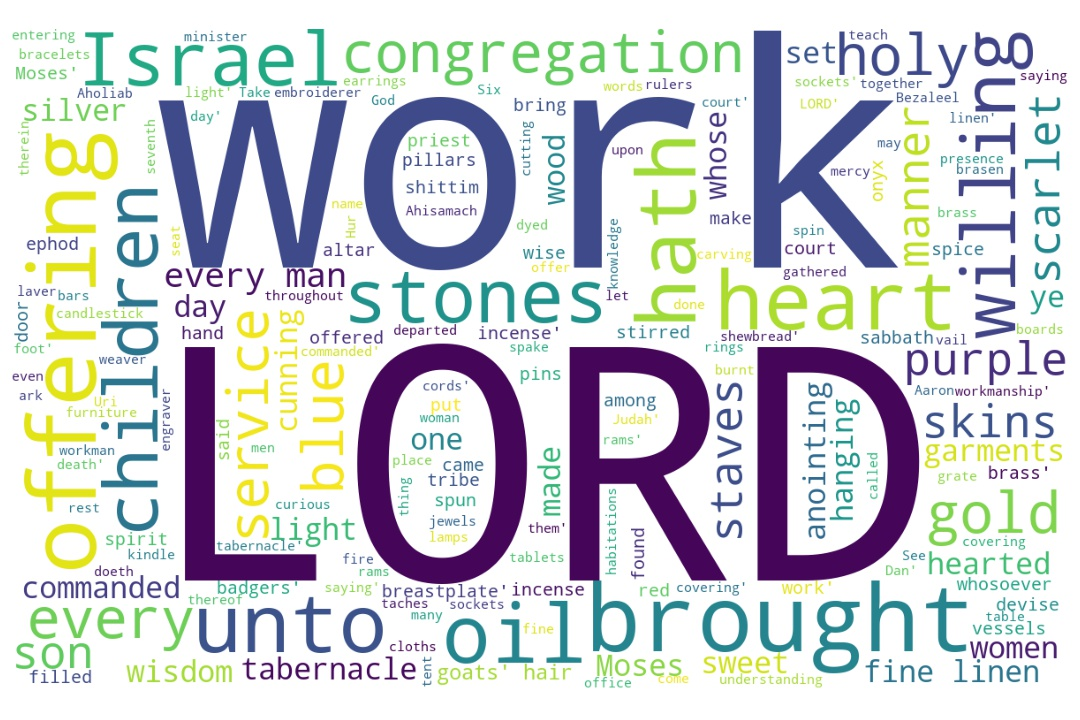
\includegraphics[width=\linewidth]{02OT-Exodus/Exodus35-WordCloud.jpg}
  \caption{Exodus 35 Word Cloud}
  \label{fig:Exodus 35 word Cloud}
\end{figure}


\marginpar{\scriptsize \centering \fcolorbox{bone}{lime}{\textbf{BUILDING A CHURCH}}\\ (Exodus 35:1-35) \begin{compactenum}[I.][8]
    \item A \textbf{Drawing} Together \index[scripture]{Exodus!Exo 35:01}(Exo 35:1)
    \item \textbf{Distinct} Rules \index[scripture]{Exodus!Exo 35:02}(Exo 35:2)
    \item \textbf{Devotion} \index[scripture]{Exodus!Exodus 35:05}(Exo 35:5)
    \item \textbf{Dedication} %\index[scripture]{Exodus!Exodus 35:02}(Exodus 35:2)
    \item A \textbf{Display} of Interest \& Involvment  \index[scripture]{Exodus!Exodus 35:10}(Exo 35:10)
    \item \textbf{Decisions} to be part of the effort %\index[scripture]{Exodus!Exodus 35:02}(Exo 35:2)
    \item \textbf{Departure} back into real life 
\end{compactenum}}










\footnote{\textcolor[cmyk]{0.99998,1,0,0}{\hyperlink{TOC}{Return to end of Table of Contents.}}}\footnote{\href{https://audiobible.com/bible/exodus_35.html}{\textcolor[cmyk]{0.99998,1,0,0}{Exodus 35 Audio}}}\textcolor[cmyk]{0.99998,1,0,0}{And Moses \fcolorbox{bone}{lime}{gathered}  \fcolorbox{bone}{bone}{all} the congregation of the children of Israel together, and said unto them, These \emph{are} the words which the LORD hath commanded, that \emph{ye} should do them.}
[2] \textcolor[cmyk]{0.99998,1,0,0}{Six days shall work be done, but on the seventh day \fcolorbox{bone}{lime}{there shall be} to you an holy day, a sabbath of rest to the LORD: whosoever doeth work therein shall be put to death.}
[3] \textcolor[cmyk]{0.99998,1,0,0}{Ye shall kindle no fire throughout your habitations upon the sabbath day.}\\
\\
\P \textcolor[cmyk]{0.99998,1,0,0}{And Moses spake unto  \fcolorbox{bone}{bone}{all} the congregation of the children of Israel, saying, This \emph{is} the thing which the LORD commanded, saying,}
[5] \textcolor[cmyk]{0.99998,1,0,0}{Take ye from among you an offering unto the LORD: whosoever \emph{is} of a \fcolorbox{bone}{lime}{willing heart}, let him bring it, an offering of the LORD; gold, and silver, and brass,}
[6] \textcolor[cmyk]{0.99998,1,0,0}{And blue, and purple, and scarlet, and fine linen, and goats' \emph{hair},}
[7] \textcolor[cmyk]{0.99998,1,0,0}{And rams' skins dyed red, and badgers' skins, and shittim wood,}
[8] \textcolor[cmyk]{0.99998,1,0,0}{And oil for the light, and spices for anointing oil, and for the sweet incense,}
[9] \textcolor[cmyk]{0.99998,1,0,0}{And onyx stones, and stones to be set for the ephod, and for the breastplate.}
[10] \textcolor[cmyk]{0.99998,1,0,0}{And every wise hearted among you shall come, and make  \fcolorbox{bone}{bone}{all} that the LORD hath commanded;}
[11] \textcolor[cmyk]{0.99998,1,0,0}{The tabernacle, his tent, and his covering, his taches, and his boards, his bars, his pillars, and his sockets,}
[12] \textcolor[cmyk]{0.99998,1,0,0}{The ark, and the staves thereof, \emph{with} the mercy seat, and the vail of the covering,}
[13] \textcolor[cmyk]{0.99998,1,0,0}{The table, and his staves, and  \fcolorbox{bone}{bone}{all} his vessels, and the shewbread,}
[14] \textcolor[cmyk]{0.99998,1,0,0}{The candlestick also for the light, and his furniture, and his lamps, with the oil for the light,}
[15] \textcolor[cmyk]{0.99998,1,0,0}{And the incense altar, and his staves, and the anointing oil, and the sweet incense, and the hanging for the door at the entering in of the tabernacle,}
[16] \textcolor[cmyk]{0.99998,1,0,0}{The altar of burnt offering, with his brasen grate, his staves, and  \fcolorbox{bone}{bone}{all} his vessels, the laver and his foot,}
[17] \textcolor[cmyk]{0.99998,1,0,0}{The hangings of the court, his pillars, and their sockets, and the hanging for the door of the court,}
[18] \textcolor[cmyk]{0.99998,1,0,0}{The pins of the tabernacle, and the pins of the court, and their cords,}
[19] \textcolor[cmyk]{0.99998,1,0,0}{The cloths of service, to do service in the holy \emph{place}, the holy garments for Aaron the priest, and the garments of his sons, to minister in the priest's office.}\\
\\
\P \textcolor[cmyk]{0.99998,1,0,0}{And  \fcolorbox{bone}{bone}{all} the congregation of the children of Israel departed from the presence of Moses.}
[21] \textcolor[cmyk]{0.99998,1,0,0}{And they came, every one whose heart stirred him up, and every one whom his spirit made willing, \emph{and} they brought the LORD'S offering to the work of the tabernacle of the congregation, and for  \fcolorbox{bone}{bone}{all} his service, and for the holy garments.}
[22] \textcolor[cmyk]{0.99998,1,0,0}{And they came, both men and women, as many as were willing hearted, \emph{and} brought bracelets, and earrings, and rings, and tablets,  \fcolorbox{bone}{bone}{all} jewels of gold: and every man that offered \emph{offered} an offering of gold unto the LORD.}
[23] \textcolor[cmyk]{0.99998,1,0,0}{And every man, with whom was found blue, and purple, and scarlet, and fine linen, and goats' \emph{hair}, and red skins of rams, and badgers' skins, brought \emph{them}.}
[24] \textcolor[cmyk]{0.99998,1,0,0}{Every one that did offer an offering of silver and brass brought the LORD'S offering: and every man, with whom was found shittim wood for any work of the service, brought \emph{it}.}
[25] \textcolor[cmyk]{0.99998,1,0,0}{And  \fcolorbox{bone}{bone}{all} the women that were wise hearted did spin with their hands, and brought that which they had spun, \emph{both} of blue, and of purple, \emph{and} of scarlet, and of fine linen.}
[26] \textcolor[cmyk]{0.99998,1,0,0}{And  \fcolorbox{bone}{bone}{all} the women whose heart stirred them up in wisdom spun goats' \emph{hair}.}
[27] \textcolor[cmyk]{0.99998,1,0,0}{And the rulers brought onyx stones, and stones to be set, for the ephod, and for the breastplate;}
[28] \textcolor[cmyk]{0.99998,1,0,0}{And spice, and oil for the light, and for the anointing oil, and for the sweet incense.}
[29] \textcolor[cmyk]{0.99998,1,0,0}{The children of Israel brought a willing offering unto the LORD, every man and woman, whose heart made them willing to bring for  \fcolorbox{bone}{bone}{all} manner of work, which the LORD had commanded to be made by the hand of Moses.}\\
\\
\P \textcolor[cmyk]{0.99998,1,0,0}{And Moses said unto the children of Israel, See, the LORD hath called by name Bezaleel the son of Uri, the son of Hur, of the tribe of Judah;}
[31] \textcolor[cmyk]{0.99998,1,0,0}{And he hath filled him with the spirit of God, in wisdom, in understanding, and in knowledge, and in  \fcolorbox{bone}{bone}{all} manner of workmanship;}
[32] \textcolor[cmyk]{0.99998,1,0,0}{And to devise curious works, to work in gold, and in silver, and in brass,}
[33] \textcolor[cmyk]{0.99998,1,0,0}{And in the cutting of stones, to set \emph{them}, and in carving of wood, to make any manner of cunning work.}
[34] \textcolor[cmyk]{0.99998,1,0,0}{And he hath put in his heart that he may teach, \emph{both} he, and Aholiab, the son of Ahisamach, of the tribe of Dan.}
[35] \textcolor[cmyk]{0.99998,1,0,0}{Them hath he filled with wisdom of heart, to work  \fcolorbox{bone}{bone}{all} manner of work, of the engraver, and of the cunning workman, and of the embroiderer, in blue, and in purple, in scarlet, and in fine linen, and of the weaver, \emph{even} of them that do any work, and of those that devise cunning work.}
\index[NWIV]{30!Exodus!Exo 35:1}\index[AWIP]{And!Exodus!Exo 35:1}\index[AWIP]{Moses!Exodus!Exo 35:1}\index[AWIP]{gathered!Exodus!Exo 35:1}\index[AWIP]{all!Exodus!Exo 35:1}\index[AWIP]{the!Exodus!Exo 35:1}\index[AWIP]{the!Exodus!Exo 35:1 (2)}\index[AWIP]{the!Exodus!Exo 35:1 (3)}\index[AWIP]{the!Exodus!Exo 35:1 (4)}\index[AWIP]{congregation!Exodus!Exo 35:1}\index[AWIP]{of!Exodus!Exo 35:1}\index[AWIP]{of!Exodus!Exo 35:1 (2)}\index[AWIP]{children!Exodus!Exo 35:1}\index[AWIP]{Israel!Exodus!Exo 35:1}\index[AWIP]{together!Exodus!Exo 35:1}\index[AWIP]{and!Exodus!Exo 35:1}\index[AWIP]{said!Exodus!Exo 35:1}\index[AWIP]{unto!Exodus!Exo 35:1}\index[AWIP]{them!Exodus!Exo 35:1}\index[AWIP]{them!Exodus!Exo 35:1 (2)}\index[AWIP]{These!Exodus!Exo 35:1}\index[AWIP]{\emph{are}!Exodus!Exo 35:1}\index[AWIP]{words!Exodus!Exo 35:1}\index[AWIP]{which!Exodus!Exo 35:1}\index[AWIP]{LORD!Exodus!Exo 35:1}\index[AWIP]{hath!Exodus!Exo 35:1}\index[AWIP]{commanded!Exodus!Exo 35:1}\index[AWIP]{that!Exodus!Exo 35:1}\index[AWIP]{\emph{ye}!Exodus!Exo 35:1}\index[AWIP]{should!Exodus!Exo 35:1}\index[AWIP]{do!Exodus!Exo 35:1}\index[AWIP]{\emph{are}!Exodus!Exo 35:1}\index[AWIP]{\emph{ye}!Exodus!Exo 35:1}

\index[NWIV]{35!Exodus!Exo 35:2}\index[AWIP]{Six!Exodus!Exo 35:2}\index[AWIP]{days!Exodus!Exo 35:2}\index[AWIP]{shall!Exodus!Exo 35:2}\index[AWIP]{shall!Exodus!Exo 35:2 (2)}\index[AWIP]{shall!Exodus!Exo 35:2 (3)}\index[AWIP]{work!Exodus!Exo 35:2}\index[AWIP]{work!Exodus!Exo 35:2 (2)}\index[AWIP]{be!Exodus!Exo 35:2}\index[AWIP]{be!Exodus!Exo 35:2 (2)}\index[AWIP]{be!Exodus!Exo 35:2 (3)}\index[AWIP]{done!Exodus!Exo 35:2}\index[AWIP]{but!Exodus!Exo 35:2}\index[AWIP]{on!Exodus!Exo 35:2}\index[AWIP]{the!Exodus!Exo 35:2}\index[AWIP]{the!Exodus!Exo 35:2 (2)}\index[AWIP]{seventh!Exodus!Exo 35:2}\index[AWIP]{day!Exodus!Exo 35:2}\index[AWIP]{day!Exodus!Exo 35:2 (2)}\index[AWIP]{there!Exodus!Exo 35:2}\index[AWIP]{to!Exodus!Exo 35:2}\index[AWIP]{to!Exodus!Exo 35:2 (2)}\index[AWIP]{to!Exodus!Exo 35:2 (3)}\index[AWIP]{you!Exodus!Exo 35:2}\index[AWIP]{an!Exodus!Exo 35:2}\index[AWIP]{holy!Exodus!Exo 35:2}\index[AWIP]{a!Exodus!Exo 35:2}\index[AWIP]{sabbath!Exodus!Exo 35:2}\index[AWIP]{of!Exodus!Exo 35:2}\index[AWIP]{rest!Exodus!Exo 35:2}\index[AWIP]{LORD!Exodus!Exo 35:2}\index[AWIP]{whosoever!Exodus!Exo 35:2}\index[AWIP]{doeth!Exodus!Exo 35:2}\index[AWIP]{therein!Exodus!Exo 35:2}\index[AWIP]{put!Exodus!Exo 35:2}\index[AWIP]{death!Exodus!Exo 35:2}

\index[NWIV]{12!Exodus!Exo 35:3}\index[AWIP]{Ye!Exodus!Exo 35:3}\index[AWIP]{shall!Exodus!Exo 35:3}\index[AWIP]{kindle!Exodus!Exo 35:3}\index[AWIP]{no!Exodus!Exo 35:3}\index[AWIP]{fire!Exodus!Exo 35:3}\index[AWIP]{throughout!Exodus!Exo 35:3}\index[AWIP]{your!Exodus!Exo 35:3}\index[AWIP]{habitations!Exodus!Exo 35:3}\index[AWIP]{upon!Exodus!Exo 35:3}\index[AWIP]{the!Exodus!Exo 35:3}\index[AWIP]{sabbath!Exodus!Exo 35:3}\index[AWIP]{day!Exodus!Exo 35:3}

\index[NWIV]{22!Exodus!Exo 35:4}\index[AWIP]{And!Exodus!Exo 35:4}\index[AWIP]{Moses!Exodus!Exo 35:4}\index[AWIP]{spake!Exodus!Exo 35:4}\index[AWIP]{unto!Exodus!Exo 35:4}\index[AWIP]{all!Exodus!Exo 35:4}\index[AWIP]{the!Exodus!Exo 35:4}\index[AWIP]{the!Exodus!Exo 35:4 (2)}\index[AWIP]{the!Exodus!Exo 35:4 (3)}\index[AWIP]{the!Exodus!Exo 35:4 (4)}\index[AWIP]{congregation!Exodus!Exo 35:4}\index[AWIP]{of!Exodus!Exo 35:4}\index[AWIP]{of!Exodus!Exo 35:4 (2)}\index[AWIP]{children!Exodus!Exo 35:4}\index[AWIP]{Israel!Exodus!Exo 35:4}\index[AWIP]{saying!Exodus!Exo 35:4}\index[AWIP]{saying!Exodus!Exo 35:4 (2)}\index[AWIP]{This!Exodus!Exo 35:4}\index[AWIP]{\emph{is}!Exodus!Exo 35:4}\index[AWIP]{thing!Exodus!Exo 35:4}\index[AWIP]{which!Exodus!Exo 35:4}\index[AWIP]{LORD!Exodus!Exo 35:4}\index[AWIP]{commanded!Exodus!Exo 35:4}\index[AWIP]{\emph{is}!Exodus!Exo 35:4}

\index[NWIV]{30!Exodus!Exo 35:5}\index[AWIP]{Take!Exodus!Exo 35:5}\index[AWIP]{ye!Exodus!Exo 35:5}\index[AWIP]{from!Exodus!Exo 35:5}\index[AWIP]{among!Exodus!Exo 35:5}\index[AWIP]{you!Exodus!Exo 35:5}\index[AWIP]{an!Exodus!Exo 35:5}\index[AWIP]{an!Exodus!Exo 35:5 (2)}\index[AWIP]{offering!Exodus!Exo 35:5}\index[AWIP]{offering!Exodus!Exo 35:5 (2)}\index[AWIP]{unto!Exodus!Exo 35:5}\index[AWIP]{the!Exodus!Exo 35:5}\index[AWIP]{the!Exodus!Exo 35:5 (2)}\index[AWIP]{LORD!Exodus!Exo 35:5}\index[AWIP]{LORD!Exodus!Exo 35:5 (2)}\index[AWIP]{whosoever!Exodus!Exo 35:5}\index[AWIP]{\emph{is}!Exodus!Exo 35:5}\index[AWIP]{of!Exodus!Exo 35:5}\index[AWIP]{of!Exodus!Exo 35:5 (2)}\index[AWIP]{a!Exodus!Exo 35:5}\index[AWIP]{willing!Exodus!Exo 35:5}\index[AWIP]{heart!Exodus!Exo 35:5}\index[AWIP]{let!Exodus!Exo 35:5}\index[AWIP]{him!Exodus!Exo 35:5}\index[AWIP]{bring!Exodus!Exo 35:5}\index[AWIP]{it!Exodus!Exo 35:5}\index[AWIP]{gold!Exodus!Exo 35:5}\index[AWIP]{and!Exodus!Exo 35:5}\index[AWIP]{and!Exodus!Exo 35:5 (2)}\index[AWIP]{silver!Exodus!Exo 35:5}\index[AWIP]{brass!Exodus!Exo 35:5}\index[AWIP]{\emph{is}!Exodus!Exo 35:5}

\index[NWIV]{12!Exodus!Exo 35:6}\index[AWIP]{And!Exodus!Exo 35:6}\index[AWIP]{blue!Exodus!Exo 35:6}\index[AWIP]{and!Exodus!Exo 35:6}\index[AWIP]{and!Exodus!Exo 35:6 (2)}\index[AWIP]{and!Exodus!Exo 35:6 (3)}\index[AWIP]{and!Exodus!Exo 35:6 (4)}\index[AWIP]{purple!Exodus!Exo 35:6}\index[AWIP]{scarlet!Exodus!Exo 35:6}\index[AWIP]{fine!Exodus!Exo 35:6}\index[AWIP]{linen!Exodus!Exo 35:6}\index[AWIP]{goats'!Exodus!Exo 35:6}\index[AWIP]{\emph{hair}!Exodus!Exo 35:6}\index[AWIP]{\emph{hair}!Exodus!Exo 35:6}

\index[NWIV]{11!Exodus!Exo 35:7}\index[AWIP]{And!Exodus!Exo 35:7}\index[AWIP]{rams'!Exodus!Exo 35:7}\index[AWIP]{skins!Exodus!Exo 35:7}\index[AWIP]{skins!Exodus!Exo 35:7 (2)}\index[AWIP]{dyed!Exodus!Exo 35:7}\index[AWIP]{red!Exodus!Exo 35:7}\index[AWIP]{and!Exodus!Exo 35:7}\index[AWIP]{and!Exodus!Exo 35:7 (2)}\index[AWIP]{badgers'!Exodus!Exo 35:7}\index[AWIP]{shittim!Exodus!Exo 35:7}\index[AWIP]{wood!Exodus!Exo 35:7}

\index[NWIV]{15!Exodus!Exo 35:8}\index[AWIP]{And!Exodus!Exo 35:8}\index[AWIP]{oil!Exodus!Exo 35:8}\index[AWIP]{oil!Exodus!Exo 35:8 (2)}\index[AWIP]{for!Exodus!Exo 35:8}\index[AWIP]{for!Exodus!Exo 35:8 (2)}\index[AWIP]{for!Exodus!Exo 35:8 (3)}\index[AWIP]{the!Exodus!Exo 35:8}\index[AWIP]{the!Exodus!Exo 35:8 (2)}\index[AWIP]{light!Exodus!Exo 35:8}\index[AWIP]{and!Exodus!Exo 35:8}\index[AWIP]{and!Exodus!Exo 35:8 (2)}\index[AWIP]{spices!Exodus!Exo 35:8}\index[AWIP]{anointing!Exodus!Exo 35:8}\index[AWIP]{sweet!Exodus!Exo 35:8}\index[AWIP]{incense!Exodus!Exo 35:8}

\index[NWIV]{15!Exodus!Exo 35:9}\index[AWIP]{And!Exodus!Exo 35:9}\index[AWIP]{onyx!Exodus!Exo 35:9}\index[AWIP]{stones!Exodus!Exo 35:9}\index[AWIP]{stones!Exodus!Exo 35:9 (2)}\index[AWIP]{and!Exodus!Exo 35:9}\index[AWIP]{and!Exodus!Exo 35:9 (2)}\index[AWIP]{to!Exodus!Exo 35:9}\index[AWIP]{be!Exodus!Exo 35:9}\index[AWIP]{set!Exodus!Exo 35:9}\index[AWIP]{for!Exodus!Exo 35:9}\index[AWIP]{for!Exodus!Exo 35:9 (2)}\index[AWIP]{the!Exodus!Exo 35:9}\index[AWIP]{the!Exodus!Exo 35:9 (2)}\index[AWIP]{ephod!Exodus!Exo 35:9}\index[AWIP]{breastplate!Exodus!Exo 35:9}

\index[NWIV]{16!Exodus!Exo 35:10}\index[AWIP]{And!Exodus!Exo 35:10}\index[AWIP]{every!Exodus!Exo 35:10}\index[AWIP]{wise!Exodus!Exo 35:10}\index[AWIP]{hearted!Exodus!Exo 35:10}\index[AWIP]{among!Exodus!Exo 35:10}\index[AWIP]{you!Exodus!Exo 35:10}\index[AWIP]{shall!Exodus!Exo 35:10}\index[AWIP]{come!Exodus!Exo 35:10}\index[AWIP]{and!Exodus!Exo 35:10}\index[AWIP]{make!Exodus!Exo 35:10}\index[AWIP]{all!Exodus!Exo 35:10}\index[AWIP]{that!Exodus!Exo 35:10}\index[AWIP]{the!Exodus!Exo 35:10}\index[AWIP]{LORD!Exodus!Exo 35:10}\index[AWIP]{hath!Exodus!Exo 35:10}\index[AWIP]{commanded!Exodus!Exo 35:10}

\index[NWIV]{19!Exodus!Exo 35:11}\index[AWIP]{The!Exodus!Exo 35:11}\index[AWIP]{tabernacle!Exodus!Exo 35:11}\index[AWIP]{his!Exodus!Exo 35:11}\index[AWIP]{his!Exodus!Exo 35:11 (2)}\index[AWIP]{his!Exodus!Exo 35:11 (3)}\index[AWIP]{his!Exodus!Exo 35:11 (4)}\index[AWIP]{his!Exodus!Exo 35:11 (5)}\index[AWIP]{his!Exodus!Exo 35:11 (6)}\index[AWIP]{his!Exodus!Exo 35:11 (7)}\index[AWIP]{tent!Exodus!Exo 35:11}\index[AWIP]{and!Exodus!Exo 35:11}\index[AWIP]{and!Exodus!Exo 35:11 (2)}\index[AWIP]{and!Exodus!Exo 35:11 (3)}\index[AWIP]{covering!Exodus!Exo 35:11}\index[AWIP]{taches!Exodus!Exo 35:11}\index[AWIP]{boards!Exodus!Exo 35:11}\index[AWIP]{bars!Exodus!Exo 35:11}\index[AWIP]{pillars!Exodus!Exo 35:11}\index[AWIP]{sockets!Exodus!Exo 35:11}

\index[NWIV]{16!Exodus!Exo 35:12}\index[AWIP]{The!Exodus!Exo 35:12}\index[AWIP]{ark!Exodus!Exo 35:12}\index[AWIP]{and!Exodus!Exo 35:12}\index[AWIP]{and!Exodus!Exo 35:12 (2)}\index[AWIP]{the!Exodus!Exo 35:12}\index[AWIP]{the!Exodus!Exo 35:12 (2)}\index[AWIP]{the!Exodus!Exo 35:12 (3)}\index[AWIP]{the!Exodus!Exo 35:12 (4)}\index[AWIP]{staves!Exodus!Exo 35:12}\index[AWIP]{thereof!Exodus!Exo 35:12}\index[AWIP]{\emph{with}!Exodus!Exo 35:12}\index[AWIP]{mercy!Exodus!Exo 35:12}\index[AWIP]{seat!Exodus!Exo 35:12}\index[AWIP]{vail!Exodus!Exo 35:12}\index[AWIP]{of!Exodus!Exo 35:12}\index[AWIP]{covering!Exodus!Exo 35:12}\index[AWIP]{\emph{with}!Exodus!Exo 35:12}

\index[NWIV]{12!Exodus!Exo 35:13}\index[AWIP]{The!Exodus!Exo 35:13}\index[AWIP]{table!Exodus!Exo 35:13}\index[AWIP]{and!Exodus!Exo 35:13}\index[AWIP]{and!Exodus!Exo 35:13 (2)}\index[AWIP]{and!Exodus!Exo 35:13 (3)}\index[AWIP]{his!Exodus!Exo 35:13}\index[AWIP]{his!Exodus!Exo 35:13 (2)}\index[AWIP]{staves!Exodus!Exo 35:13}\index[AWIP]{all!Exodus!Exo 35:13}\index[AWIP]{vessels!Exodus!Exo 35:13}\index[AWIP]{the!Exodus!Exo 35:13}\index[AWIP]{shewbread!Exodus!Exo 35:13}

\index[NWIV]{18!Exodus!Exo 35:14}\index[AWIP]{The!Exodus!Exo 35:14}\index[AWIP]{candlestick!Exodus!Exo 35:14}\index[AWIP]{also!Exodus!Exo 35:14}\index[AWIP]{for!Exodus!Exo 35:14}\index[AWIP]{for!Exodus!Exo 35:14 (2)}\index[AWIP]{the!Exodus!Exo 35:14}\index[AWIP]{the!Exodus!Exo 35:14 (2)}\index[AWIP]{the!Exodus!Exo 35:14 (3)}\index[AWIP]{light!Exodus!Exo 35:14}\index[AWIP]{light!Exodus!Exo 35:14 (2)}\index[AWIP]{and!Exodus!Exo 35:14}\index[AWIP]{and!Exodus!Exo 35:14 (2)}\index[AWIP]{his!Exodus!Exo 35:14}\index[AWIP]{his!Exodus!Exo 35:14 (2)}\index[AWIP]{furniture!Exodus!Exo 35:14}\index[AWIP]{lamps!Exodus!Exo 35:14}\index[AWIP]{with!Exodus!Exo 35:14}\index[AWIP]{oil!Exodus!Exo 35:14}

\index[NWIV]{28!Exodus!Exo 35:15}\index[AWIP]{And!Exodus!Exo 35:15}\index[AWIP]{the!Exodus!Exo 35:15}\index[AWIP]{the!Exodus!Exo 35:15 (2)}\index[AWIP]{the!Exodus!Exo 35:15 (3)}\index[AWIP]{the!Exodus!Exo 35:15 (4)}\index[AWIP]{the!Exodus!Exo 35:15 (5)}\index[AWIP]{the!Exodus!Exo 35:15 (6)}\index[AWIP]{the!Exodus!Exo 35:15 (7)}\index[AWIP]{incense!Exodus!Exo 35:15}\index[AWIP]{incense!Exodus!Exo 35:15 (2)}\index[AWIP]{altar!Exodus!Exo 35:15}\index[AWIP]{and!Exodus!Exo 35:15}\index[AWIP]{and!Exodus!Exo 35:15 (2)}\index[AWIP]{and!Exodus!Exo 35:15 (3)}\index[AWIP]{and!Exodus!Exo 35:15 (4)}\index[AWIP]{his!Exodus!Exo 35:15}\index[AWIP]{staves!Exodus!Exo 35:15}\index[AWIP]{anointing!Exodus!Exo 35:15}\index[AWIP]{oil!Exodus!Exo 35:15}\index[AWIP]{sweet!Exodus!Exo 35:15}\index[AWIP]{hanging!Exodus!Exo 35:15}\index[AWIP]{for!Exodus!Exo 35:15}\index[AWIP]{door!Exodus!Exo 35:15}\index[AWIP]{at!Exodus!Exo 35:15}\index[AWIP]{entering!Exodus!Exo 35:15}\index[AWIP]{in!Exodus!Exo 35:15}\index[AWIP]{of!Exodus!Exo 35:15}\index[AWIP]{tabernacle!Exodus!Exo 35:15}

\index[NWIV]{20!Exodus!Exo 35:16}\index[AWIP]{The!Exodus!Exo 35:16}\index[AWIP]{altar!Exodus!Exo 35:16}\index[AWIP]{of!Exodus!Exo 35:16}\index[AWIP]{burnt!Exodus!Exo 35:16}\index[AWIP]{offering!Exodus!Exo 35:16}\index[AWIP]{with!Exodus!Exo 35:16}\index[AWIP]{his!Exodus!Exo 35:16}\index[AWIP]{his!Exodus!Exo 35:16 (2)}\index[AWIP]{his!Exodus!Exo 35:16 (3)}\index[AWIP]{his!Exodus!Exo 35:16 (4)}\index[AWIP]{brasen!Exodus!Exo 35:16}\index[AWIP]{grate!Exodus!Exo 35:16}\index[AWIP]{staves!Exodus!Exo 35:16}\index[AWIP]{and!Exodus!Exo 35:16}\index[AWIP]{and!Exodus!Exo 35:16 (2)}\index[AWIP]{all!Exodus!Exo 35:16}\index[AWIP]{vessels!Exodus!Exo 35:16}\index[AWIP]{the!Exodus!Exo 35:16}\index[AWIP]{laver!Exodus!Exo 35:16}\index[AWIP]{foot!Exodus!Exo 35:16}

\index[NWIV]{19!Exodus!Exo 35:17}\index[AWIP]{The!Exodus!Exo 35:17}\index[AWIP]{hangings!Exodus!Exo 35:17}\index[AWIP]{of!Exodus!Exo 35:17}\index[AWIP]{of!Exodus!Exo 35:17 (2)}\index[AWIP]{the!Exodus!Exo 35:17}\index[AWIP]{the!Exodus!Exo 35:17 (2)}\index[AWIP]{the!Exodus!Exo 35:17 (3)}\index[AWIP]{the!Exodus!Exo 35:17 (4)}\index[AWIP]{court!Exodus!Exo 35:17}\index[AWIP]{court!Exodus!Exo 35:17 (2)}\index[AWIP]{his!Exodus!Exo 35:17}\index[AWIP]{pillars!Exodus!Exo 35:17}\index[AWIP]{and!Exodus!Exo 35:17}\index[AWIP]{and!Exodus!Exo 35:17 (2)}\index[AWIP]{their!Exodus!Exo 35:17}\index[AWIP]{sockets!Exodus!Exo 35:17}\index[AWIP]{hanging!Exodus!Exo 35:17}\index[AWIP]{for!Exodus!Exo 35:17}\index[AWIP]{door!Exodus!Exo 35:17}

\index[NWIV]{14!Exodus!Exo 35:18}\index[AWIP]{The!Exodus!Exo 35:18}\index[AWIP]{pins!Exodus!Exo 35:18}\index[AWIP]{pins!Exodus!Exo 35:18 (2)}\index[AWIP]{of!Exodus!Exo 35:18}\index[AWIP]{of!Exodus!Exo 35:18 (2)}\index[AWIP]{the!Exodus!Exo 35:18}\index[AWIP]{the!Exodus!Exo 35:18 (2)}\index[AWIP]{the!Exodus!Exo 35:18 (3)}\index[AWIP]{tabernacle!Exodus!Exo 35:18}\index[AWIP]{and!Exodus!Exo 35:18}\index[AWIP]{and!Exodus!Exo 35:18 (2)}\index[AWIP]{court!Exodus!Exo 35:18}\index[AWIP]{their!Exodus!Exo 35:18}\index[AWIP]{cords!Exodus!Exo 35:18}

\index[NWIV]{30!Exodus!Exo 35:19}\index[AWIP]{The!Exodus!Exo 35:19}\index[AWIP]{cloths!Exodus!Exo 35:19}\index[AWIP]{of!Exodus!Exo 35:19}\index[AWIP]{of!Exodus!Exo 35:19 (2)}\index[AWIP]{service!Exodus!Exo 35:19}\index[AWIP]{service!Exodus!Exo 35:19 (2)}\index[AWIP]{to!Exodus!Exo 35:19}\index[AWIP]{to!Exodus!Exo 35:19 (2)}\index[AWIP]{do!Exodus!Exo 35:19}\index[AWIP]{in!Exodus!Exo 35:19}\index[AWIP]{in!Exodus!Exo 35:19 (2)}\index[AWIP]{the!Exodus!Exo 35:19}\index[AWIP]{the!Exodus!Exo 35:19 (2)}\index[AWIP]{the!Exodus!Exo 35:19 (3)}\index[AWIP]{the!Exodus!Exo 35:19 (4)}\index[AWIP]{the!Exodus!Exo 35:19 (5)}\index[AWIP]{holy!Exodus!Exo 35:19}\index[AWIP]{holy!Exodus!Exo 35:19 (2)}\index[AWIP]{\emph{place}!Exodus!Exo 35:19}\index[AWIP]{garments!Exodus!Exo 35:19}\index[AWIP]{garments!Exodus!Exo 35:19 (2)}\index[AWIP]{for!Exodus!Exo 35:19}\index[AWIP]{Aaron!Exodus!Exo 35:19}\index[AWIP]{priest!Exodus!Exo 35:19}\index[AWIP]{and!Exodus!Exo 35:19}\index[AWIP]{his!Exodus!Exo 35:19}\index[AWIP]{sons!Exodus!Exo 35:19}\index[AWIP]{minister!Exodus!Exo 35:19}\index[AWIP]{priest's!Exodus!Exo 35:19}\index[AWIP]{office!Exodus!Exo 35:19}\index[AWIP]{\emph{place}!Exodus!Exo 35:19}

\index[NWIV]{15!Exodus!Exo 35:20}\index[AWIP]{And!Exodus!Exo 35:20}\index[AWIP]{all!Exodus!Exo 35:20}\index[AWIP]{the!Exodus!Exo 35:20}\index[AWIP]{the!Exodus!Exo 35:20 (2)}\index[AWIP]{the!Exodus!Exo 35:20 (3)}\index[AWIP]{congregation!Exodus!Exo 35:20}\index[AWIP]{of!Exodus!Exo 35:20}\index[AWIP]{of!Exodus!Exo 35:20 (2)}\index[AWIP]{of!Exodus!Exo 35:20 (3)}\index[AWIP]{children!Exodus!Exo 35:20}\index[AWIP]{Israel!Exodus!Exo 35:20}\index[AWIP]{departed!Exodus!Exo 35:20}\index[AWIP]{from!Exodus!Exo 35:20}\index[AWIP]{presence!Exodus!Exo 35:20}\index[AWIP]{Moses!Exodus!Exo 35:20}

\index[NWIV]{43!Exodus!Exo 35:21}\index[AWIP]{And!Exodus!Exo 35:21}\index[AWIP]{they!Exodus!Exo 35:21}\index[AWIP]{they!Exodus!Exo 35:21 (2)}\index[AWIP]{came!Exodus!Exo 35:21}\index[AWIP]{every!Exodus!Exo 35:21}\index[AWIP]{every!Exodus!Exo 35:21 (2)}\index[AWIP]{one!Exodus!Exo 35:21}\index[AWIP]{one!Exodus!Exo 35:21 (2)}\index[AWIP]{whose!Exodus!Exo 35:21}\index[AWIP]{heart!Exodus!Exo 35:21}\index[AWIP]{stirred!Exodus!Exo 35:21}\index[AWIP]{him!Exodus!Exo 35:21}\index[AWIP]{up!Exodus!Exo 35:21}\index[AWIP]{and!Exodus!Exo 35:21}\index[AWIP]{and!Exodus!Exo 35:21 (2)}\index[AWIP]{and!Exodus!Exo 35:21 (3)}\index[AWIP]{whom!Exodus!Exo 35:21}\index[AWIP]{his!Exodus!Exo 35:21}\index[AWIP]{his!Exodus!Exo 35:21 (2)}\index[AWIP]{spirit!Exodus!Exo 35:21}\index[AWIP]{made!Exodus!Exo 35:21}\index[AWIP]{willing!Exodus!Exo 35:21}\index[AWIP]{\emph{and}!Exodus!Exo 35:21}\index[AWIP]{brought!Exodus!Exo 35:21}\index[AWIP]{the!Exodus!Exo 35:21}\index[AWIP]{the!Exodus!Exo 35:21 (2)}\index[AWIP]{the!Exodus!Exo 35:21 (3)}\index[AWIP]{the!Exodus!Exo 35:21 (4)}\index[AWIP]{the!Exodus!Exo 35:21 (5)}\index[AWIP]{LORD'S!Exodus!Exo 35:21}\index[AWIP]{offering!Exodus!Exo 35:21}\index[AWIP]{to!Exodus!Exo 35:21}\index[AWIP]{work!Exodus!Exo 35:21}\index[AWIP]{of!Exodus!Exo 35:21}\index[AWIP]{of!Exodus!Exo 35:21 (2)}\index[AWIP]{tabernacle!Exodus!Exo 35:21}\index[AWIP]{congregation!Exodus!Exo 35:21}\index[AWIP]{for!Exodus!Exo 35:21}\index[AWIP]{for!Exodus!Exo 35:21 (2)}\index[AWIP]{all!Exodus!Exo 35:21}\index[AWIP]{service!Exodus!Exo 35:21}\index[AWIP]{holy!Exodus!Exo 35:21}\index[AWIP]{garments!Exodus!Exo 35:21}\index[AWIP]{\emph{and}!Exodus!Exo 35:21}

\index[NWIV]{39!Exodus!Exo 35:22}\index[AWIP]{And!Exodus!Exo 35:22}\index[AWIP]{they!Exodus!Exo 35:22}\index[AWIP]{came!Exodus!Exo 35:22}\index[AWIP]{both!Exodus!Exo 35:22}\index[AWIP]{men!Exodus!Exo 35:22}\index[AWIP]{and!Exodus!Exo 35:22}\index[AWIP]{and!Exodus!Exo 35:22 (2)}\index[AWIP]{and!Exodus!Exo 35:22 (3)}\index[AWIP]{and!Exodus!Exo 35:22 (4)}\index[AWIP]{and!Exodus!Exo 35:22 (5)}\index[AWIP]{women!Exodus!Exo 35:22}\index[AWIP]{as!Exodus!Exo 35:22}\index[AWIP]{as!Exodus!Exo 35:22 (2)}\index[AWIP]{many!Exodus!Exo 35:22}\index[AWIP]{were!Exodus!Exo 35:22}\index[AWIP]{willing!Exodus!Exo 35:22}\index[AWIP]{hearted!Exodus!Exo 35:22}\index[AWIP]{\emph{and}!Exodus!Exo 35:22}\index[AWIP]{brought!Exodus!Exo 35:22}\index[AWIP]{bracelets!Exodus!Exo 35:22}\index[AWIP]{earrings!Exodus!Exo 35:22}\index[AWIP]{rings!Exodus!Exo 35:22}\index[AWIP]{tablets!Exodus!Exo 35:22}\index[AWIP]{all!Exodus!Exo 35:22}\index[AWIP]{jewels!Exodus!Exo 35:22}\index[AWIP]{of!Exodus!Exo 35:22}\index[AWIP]{of!Exodus!Exo 35:22 (2)}\index[AWIP]{gold!Exodus!Exo 35:22}\index[AWIP]{gold!Exodus!Exo 35:22 (2)}\index[AWIP]{every!Exodus!Exo 35:22}\index[AWIP]{man!Exodus!Exo 35:22}\index[AWIP]{that!Exodus!Exo 35:22}\index[AWIP]{offered!Exodus!Exo 35:22}\index[AWIP]{\emph{offered}!Exodus!Exo 35:22}\index[AWIP]{an!Exodus!Exo 35:22}\index[AWIP]{offering!Exodus!Exo 35:22}\index[AWIP]{unto!Exodus!Exo 35:22}\index[AWIP]{the!Exodus!Exo 35:22}\index[AWIP]{LORD!Exodus!Exo 35:22}\index[AWIP]{\emph{and}!Exodus!Exo 35:22}\index[AWIP]{\emph{offered}!Exodus!Exo 35:22}

\index[NWIV]{28!Exodus!Exo 35:23}\index[AWIP]{And!Exodus!Exo 35:23}\index[AWIP]{every!Exodus!Exo 35:23}\index[AWIP]{man!Exodus!Exo 35:23}\index[AWIP]{with!Exodus!Exo 35:23}\index[AWIP]{whom!Exodus!Exo 35:23}\index[AWIP]{was!Exodus!Exo 35:23}\index[AWIP]{found!Exodus!Exo 35:23}\index[AWIP]{blue!Exodus!Exo 35:23}\index[AWIP]{and!Exodus!Exo 35:23}\index[AWIP]{and!Exodus!Exo 35:23 (2)}\index[AWIP]{and!Exodus!Exo 35:23 (3)}\index[AWIP]{and!Exodus!Exo 35:23 (4)}\index[AWIP]{and!Exodus!Exo 35:23 (5)}\index[AWIP]{and!Exodus!Exo 35:23 (6)}\index[AWIP]{purple!Exodus!Exo 35:23}\index[AWIP]{scarlet!Exodus!Exo 35:23}\index[AWIP]{fine!Exodus!Exo 35:23}\index[AWIP]{linen!Exodus!Exo 35:23}\index[AWIP]{goats'!Exodus!Exo 35:23}\index[AWIP]{\emph{hair}!Exodus!Exo 35:23}\index[AWIP]{red!Exodus!Exo 35:23}\index[AWIP]{skins!Exodus!Exo 35:23}\index[AWIP]{skins!Exodus!Exo 35:23 (2)}\index[AWIP]{of!Exodus!Exo 35:23}\index[AWIP]{rams!Exodus!Exo 35:23}\index[AWIP]{badgers'!Exodus!Exo 35:23}\index[AWIP]{brought!Exodus!Exo 35:23}\index[AWIP]{\emph{them}!Exodus!Exo 35:23}\index[AWIP]{\emph{hair}!Exodus!Exo 35:23}\index[AWIP]{\emph{them}!Exodus!Exo 35:23}

\index[NWIV]{32!Exodus!Exo 35:24}\index[AWIP]{Every!Exodus!Exo 35:24}\index[AWIP]{one!Exodus!Exo 35:24}\index[AWIP]{that!Exodus!Exo 35:24}\index[AWIP]{did!Exodus!Exo 35:24}\index[AWIP]{offer!Exodus!Exo 35:24}\index[AWIP]{an!Exodus!Exo 35:24}\index[AWIP]{offering!Exodus!Exo 35:24}\index[AWIP]{offering!Exodus!Exo 35:24 (2)}\index[AWIP]{of!Exodus!Exo 35:24}\index[AWIP]{of!Exodus!Exo 35:24 (2)}\index[AWIP]{silver!Exodus!Exo 35:24}\index[AWIP]{and!Exodus!Exo 35:24}\index[AWIP]{and!Exodus!Exo 35:24 (2)}\index[AWIP]{brass!Exodus!Exo 35:24}\index[AWIP]{brought!Exodus!Exo 35:24}\index[AWIP]{brought!Exodus!Exo 35:24 (2)}\index[AWIP]{the!Exodus!Exo 35:24}\index[AWIP]{the!Exodus!Exo 35:24 (2)}\index[AWIP]{LORD'S!Exodus!Exo 35:24}\index[AWIP]{every!Exodus!Exo 35:24}\index[AWIP]{man!Exodus!Exo 35:24}\index[AWIP]{with!Exodus!Exo 35:24}\index[AWIP]{whom!Exodus!Exo 35:24}\index[AWIP]{was!Exodus!Exo 35:24}\index[AWIP]{found!Exodus!Exo 35:24}\index[AWIP]{shittim!Exodus!Exo 35:24}\index[AWIP]{wood!Exodus!Exo 35:24}\index[AWIP]{for!Exodus!Exo 35:24}\index[AWIP]{any!Exodus!Exo 35:24}\index[AWIP]{work!Exodus!Exo 35:24}\index[AWIP]{service!Exodus!Exo 35:24}\index[AWIP]{\emph{it}!Exodus!Exo 35:24}\index[AWIP]{\emph{it}!Exodus!Exo 35:24}

\index[NWIV]{33!Exodus!Exo 35:25}\index[AWIP]{And!Exodus!Exo 35:25}\index[AWIP]{all!Exodus!Exo 35:25}\index[AWIP]{the!Exodus!Exo 35:25}\index[AWIP]{women!Exodus!Exo 35:25}\index[AWIP]{that!Exodus!Exo 35:25}\index[AWIP]{that!Exodus!Exo 35:25 (2)}\index[AWIP]{were!Exodus!Exo 35:25}\index[AWIP]{wise!Exodus!Exo 35:25}\index[AWIP]{hearted!Exodus!Exo 35:25}\index[AWIP]{did!Exodus!Exo 35:25}\index[AWIP]{spin!Exodus!Exo 35:25}\index[AWIP]{with!Exodus!Exo 35:25}\index[AWIP]{their!Exodus!Exo 35:25}\index[AWIP]{hands!Exodus!Exo 35:25}\index[AWIP]{and!Exodus!Exo 35:25}\index[AWIP]{and!Exodus!Exo 35:25 (2)}\index[AWIP]{and!Exodus!Exo 35:25 (3)}\index[AWIP]{brought!Exodus!Exo 35:25}\index[AWIP]{which!Exodus!Exo 35:25}\index[AWIP]{they!Exodus!Exo 35:25}\index[AWIP]{had!Exodus!Exo 35:25}\index[AWIP]{spun!Exodus!Exo 35:25}\index[AWIP]{\emph{both}!Exodus!Exo 35:25}\index[AWIP]{of!Exodus!Exo 35:25}\index[AWIP]{of!Exodus!Exo 35:25 (2)}\index[AWIP]{of!Exodus!Exo 35:25 (3)}\index[AWIP]{of!Exodus!Exo 35:25 (4)}\index[AWIP]{blue!Exodus!Exo 35:25}\index[AWIP]{purple!Exodus!Exo 35:25}\index[AWIP]{\emph{and}!Exodus!Exo 35:25}\index[AWIP]{scarlet!Exodus!Exo 35:25}\index[AWIP]{fine!Exodus!Exo 35:25}\index[AWIP]{linen!Exodus!Exo 35:25}\index[AWIP]{\emph{both}!Exodus!Exo 35:25}\index[AWIP]{\emph{and}!Exodus!Exo 35:25}

\index[NWIV]{14!Exodus!Exo 35:26}\index[AWIP]{And!Exodus!Exo 35:26}\index[AWIP]{all!Exodus!Exo 35:26}\index[AWIP]{the!Exodus!Exo 35:26}\index[AWIP]{women!Exodus!Exo 35:26}\index[AWIP]{whose!Exodus!Exo 35:26}\index[AWIP]{heart!Exodus!Exo 35:26}\index[AWIP]{stirred!Exodus!Exo 35:26}\index[AWIP]{them!Exodus!Exo 35:26}\index[AWIP]{up!Exodus!Exo 35:26}\index[AWIP]{in!Exodus!Exo 35:26}\index[AWIP]{wisdom!Exodus!Exo 35:26}\index[AWIP]{spun!Exodus!Exo 35:26}\index[AWIP]{goats'!Exodus!Exo 35:26}\index[AWIP]{\emph{hair}!Exodus!Exo 35:26}\index[AWIP]{\emph{hair}!Exodus!Exo 35:26}

\index[NWIV]{18!Exodus!Exo 35:27}\index[AWIP]{And!Exodus!Exo 35:27}\index[AWIP]{the!Exodus!Exo 35:27}\index[AWIP]{the!Exodus!Exo 35:27 (2)}\index[AWIP]{the!Exodus!Exo 35:27 (3)}\index[AWIP]{rulers!Exodus!Exo 35:27}\index[AWIP]{brought!Exodus!Exo 35:27}\index[AWIP]{onyx!Exodus!Exo 35:27}\index[AWIP]{stones!Exodus!Exo 35:27}\index[AWIP]{stones!Exodus!Exo 35:27 (2)}\index[AWIP]{and!Exodus!Exo 35:27}\index[AWIP]{and!Exodus!Exo 35:27 (2)}\index[AWIP]{to!Exodus!Exo 35:27}\index[AWIP]{be!Exodus!Exo 35:27}\index[AWIP]{set!Exodus!Exo 35:27}\index[AWIP]{for!Exodus!Exo 35:27}\index[AWIP]{for!Exodus!Exo 35:27 (2)}\index[AWIP]{ephod!Exodus!Exo 35:27}\index[AWIP]{breastplate!Exodus!Exo 35:27}

\index[NWIV]{17!Exodus!Exo 35:28}\index[AWIP]{And!Exodus!Exo 35:28}\index[AWIP]{spice!Exodus!Exo 35:28}\index[AWIP]{and!Exodus!Exo 35:28}\index[AWIP]{and!Exodus!Exo 35:28 (2)}\index[AWIP]{and!Exodus!Exo 35:28 (3)}\index[AWIP]{oil!Exodus!Exo 35:28}\index[AWIP]{oil!Exodus!Exo 35:28 (2)}\index[AWIP]{for!Exodus!Exo 35:28}\index[AWIP]{for!Exodus!Exo 35:28 (2)}\index[AWIP]{for!Exodus!Exo 35:28 (3)}\index[AWIP]{the!Exodus!Exo 35:28}\index[AWIP]{the!Exodus!Exo 35:28 (2)}\index[AWIP]{the!Exodus!Exo 35:28 (3)}\index[AWIP]{light!Exodus!Exo 35:28}\index[AWIP]{anointing!Exodus!Exo 35:28}\index[AWIP]{sweet!Exodus!Exo 35:28}\index[AWIP]{incense!Exodus!Exo 35:28}

\index[NWIV]{40!Exodus!Exo 35:29}\index[AWIP]{The!Exodus!Exo 35:29}\index[AWIP]{children!Exodus!Exo 35:29}\index[AWIP]{of!Exodus!Exo 35:29}\index[AWIP]{of!Exodus!Exo 35:29 (2)}\index[AWIP]{of!Exodus!Exo 35:29 (3)}\index[AWIP]{Israel!Exodus!Exo 35:29}\index[AWIP]{brought!Exodus!Exo 35:29}\index[AWIP]{a!Exodus!Exo 35:29}\index[AWIP]{willing!Exodus!Exo 35:29}\index[AWIP]{willing!Exodus!Exo 35:29 (2)}\index[AWIP]{offering!Exodus!Exo 35:29}\index[AWIP]{unto!Exodus!Exo 35:29}\index[AWIP]{the!Exodus!Exo 35:29}\index[AWIP]{the!Exodus!Exo 35:29 (2)}\index[AWIP]{the!Exodus!Exo 35:29 (3)}\index[AWIP]{LORD!Exodus!Exo 35:29}\index[AWIP]{LORD!Exodus!Exo 35:29 (2)}\index[AWIP]{every!Exodus!Exo 35:29}\index[AWIP]{man!Exodus!Exo 35:29}\index[AWIP]{and!Exodus!Exo 35:29}\index[AWIP]{woman!Exodus!Exo 35:29}\index[AWIP]{whose!Exodus!Exo 35:29}\index[AWIP]{heart!Exodus!Exo 35:29}\index[AWIP]{made!Exodus!Exo 35:29}\index[AWIP]{made!Exodus!Exo 35:29 (2)}\index[AWIP]{them!Exodus!Exo 35:29}\index[AWIP]{to!Exodus!Exo 35:29}\index[AWIP]{to!Exodus!Exo 35:29 (2)}\index[AWIP]{bring!Exodus!Exo 35:29}\index[AWIP]{for!Exodus!Exo 35:29}\index[AWIP]{all!Exodus!Exo 35:29}\index[AWIP]{manner!Exodus!Exo 35:29}\index[AWIP]{work!Exodus!Exo 35:29}\index[AWIP]{which!Exodus!Exo 35:29}\index[AWIP]{had!Exodus!Exo 35:29}\index[AWIP]{commanded!Exodus!Exo 35:29}\index[AWIP]{be!Exodus!Exo 35:29}\index[AWIP]{by!Exodus!Exo 35:29}\index[AWIP]{hand!Exodus!Exo 35:29}\index[AWIP]{Moses!Exodus!Exo 35:29}

\index[NWIV]{29!Exodus!Exo 35:30}\index[AWIP]{And!Exodus!Exo 35:30}\index[AWIP]{Moses!Exodus!Exo 35:30}\index[AWIP]{said!Exodus!Exo 35:30}\index[AWIP]{unto!Exodus!Exo 35:30}\index[AWIP]{the!Exodus!Exo 35:30}\index[AWIP]{the!Exodus!Exo 35:30 (2)}\index[AWIP]{the!Exodus!Exo 35:30 (3)}\index[AWIP]{the!Exodus!Exo 35:30 (4)}\index[AWIP]{the!Exodus!Exo 35:30 (5)}\index[AWIP]{children!Exodus!Exo 35:30}\index[AWIP]{of!Exodus!Exo 35:30}\index[AWIP]{of!Exodus!Exo 35:30 (2)}\index[AWIP]{of!Exodus!Exo 35:30 (3)}\index[AWIP]{of!Exodus!Exo 35:30 (4)}\index[AWIP]{of!Exodus!Exo 35:30 (5)}\index[AWIP]{Israel!Exodus!Exo 35:30}\index[AWIP]{See!Exodus!Exo 35:30}\index[AWIP]{LORD!Exodus!Exo 35:30}\index[AWIP]{hath!Exodus!Exo 35:30}\index[AWIP]{called!Exodus!Exo 35:30}\index[AWIP]{by!Exodus!Exo 35:30}\index[AWIP]{name!Exodus!Exo 35:30}\index[AWIP]{Bezaleel!Exodus!Exo 35:30}\index[AWIP]{son!Exodus!Exo 35:30}\index[AWIP]{son!Exodus!Exo 35:30 (2)}\index[AWIP]{Uri!Exodus!Exo 35:30}\index[AWIP]{Hur!Exodus!Exo 35:30}\index[AWIP]{tribe!Exodus!Exo 35:30}\index[AWIP]{Judah!Exodus!Exo 35:30}

\index[NWIV]{23!Exodus!Exo 35:31}\index[AWIP]{And!Exodus!Exo 35:31}\index[AWIP]{he!Exodus!Exo 35:31}\index[AWIP]{hath!Exodus!Exo 35:31}\index[AWIP]{filled!Exodus!Exo 35:31}\index[AWIP]{him!Exodus!Exo 35:31}\index[AWIP]{with!Exodus!Exo 35:31}\index[AWIP]{the!Exodus!Exo 35:31}\index[AWIP]{spirit!Exodus!Exo 35:31}\index[AWIP]{of!Exodus!Exo 35:31}\index[AWIP]{of!Exodus!Exo 35:31 (2)}\index[AWIP]{God!Exodus!Exo 35:31}\index[AWIP]{in!Exodus!Exo 35:31}\index[AWIP]{in!Exodus!Exo 35:31 (2)}\index[AWIP]{in!Exodus!Exo 35:31 (3)}\index[AWIP]{in!Exodus!Exo 35:31 (4)}\index[AWIP]{wisdom!Exodus!Exo 35:31}\index[AWIP]{understanding!Exodus!Exo 35:31}\index[AWIP]{and!Exodus!Exo 35:31}\index[AWIP]{and!Exodus!Exo 35:31 (2)}\index[AWIP]{knowledge!Exodus!Exo 35:31}\index[AWIP]{all!Exodus!Exo 35:31}\index[AWIP]{manner!Exodus!Exo 35:31}\index[AWIP]{workmanship!Exodus!Exo 35:31}

\index[NWIV]{15!Exodus!Exo 35:32}\index[AWIP]{And!Exodus!Exo 35:32}\index[AWIP]{to!Exodus!Exo 35:32}\index[AWIP]{to!Exodus!Exo 35:32 (2)}\index[AWIP]{devise!Exodus!Exo 35:32}\index[AWIP]{curious!Exodus!Exo 35:32}\index[AWIP]{works!Exodus!Exo 35:32}\index[AWIP]{work!Exodus!Exo 35:32}\index[AWIP]{in!Exodus!Exo 35:32}\index[AWIP]{in!Exodus!Exo 35:32 (2)}\index[AWIP]{in!Exodus!Exo 35:32 (3)}\index[AWIP]{gold!Exodus!Exo 35:32}\index[AWIP]{and!Exodus!Exo 35:32}\index[AWIP]{and!Exodus!Exo 35:32 (2)}\index[AWIP]{silver!Exodus!Exo 35:32}\index[AWIP]{brass!Exodus!Exo 35:32}

\index[NWIV]{21!Exodus!Exo 35:33}\index[AWIP]{And!Exodus!Exo 35:33}\index[AWIP]{in!Exodus!Exo 35:33}\index[AWIP]{in!Exodus!Exo 35:33 (2)}\index[AWIP]{the!Exodus!Exo 35:33}\index[AWIP]{cutting!Exodus!Exo 35:33}\index[AWIP]{of!Exodus!Exo 35:33}\index[AWIP]{of!Exodus!Exo 35:33 (2)}\index[AWIP]{of!Exodus!Exo 35:33 (3)}\index[AWIP]{stones!Exodus!Exo 35:33}\index[AWIP]{to!Exodus!Exo 35:33}\index[AWIP]{to!Exodus!Exo 35:33 (2)}\index[AWIP]{set!Exodus!Exo 35:33}\index[AWIP]{\emph{them}!Exodus!Exo 35:33}\index[AWIP]{and!Exodus!Exo 35:33}\index[AWIP]{carving!Exodus!Exo 35:33}\index[AWIP]{wood!Exodus!Exo 35:33}\index[AWIP]{make!Exodus!Exo 35:33}\index[AWIP]{any!Exodus!Exo 35:33}\index[AWIP]{manner!Exodus!Exo 35:33}\index[AWIP]{cunning!Exodus!Exo 35:33}\index[AWIP]{work!Exodus!Exo 35:33}\index[AWIP]{\emph{them}!Exodus!Exo 35:33}

\index[NWIV]{24!Exodus!Exo 35:34}\index[AWIP]{And!Exodus!Exo 35:34}\index[AWIP]{he!Exodus!Exo 35:34}\index[AWIP]{he!Exodus!Exo 35:34 (2)}\index[AWIP]{he!Exodus!Exo 35:34 (3)}\index[AWIP]{hath!Exodus!Exo 35:34}\index[AWIP]{put!Exodus!Exo 35:34}\index[AWIP]{in!Exodus!Exo 35:34}\index[AWIP]{his!Exodus!Exo 35:34}\index[AWIP]{heart!Exodus!Exo 35:34}\index[AWIP]{that!Exodus!Exo 35:34}\index[AWIP]{may!Exodus!Exo 35:34}\index[AWIP]{teach!Exodus!Exo 35:34}\index[AWIP]{\emph{both}!Exodus!Exo 35:34}\index[AWIP]{and!Exodus!Exo 35:34}\index[AWIP]{Aholiab!Exodus!Exo 35:34}\index[AWIP]{the!Exodus!Exo 35:34}\index[AWIP]{the!Exodus!Exo 35:34 (2)}\index[AWIP]{son!Exodus!Exo 35:34}\index[AWIP]{of!Exodus!Exo 35:34}\index[AWIP]{of!Exodus!Exo 35:34 (2)}\index[AWIP]{of!Exodus!Exo 35:34 (3)}\index[AWIP]{Ahisamach!Exodus!Exo 35:34}\index[AWIP]{tribe!Exodus!Exo 35:34}\index[AWIP]{Dan!Exodus!Exo 35:34}\index[AWIP]{\emph{both}!Exodus!Exo 35:34}

\index[NWIV]{55!Exodus!Exo 35:35}\index[AWIP]{Them!Exodus!Exo 35:35}\index[AWIP]{hath!Exodus!Exo 35:35}\index[AWIP]{he!Exodus!Exo 35:35}\index[AWIP]{filled!Exodus!Exo 35:35}\index[AWIP]{with!Exodus!Exo 35:35}\index[AWIP]{wisdom!Exodus!Exo 35:35}\index[AWIP]{of!Exodus!Exo 35:35}\index[AWIP]{of!Exodus!Exo 35:35 (2)}\index[AWIP]{of!Exodus!Exo 35:35 (3)}\index[AWIP]{of!Exodus!Exo 35:35 (4)}\index[AWIP]{of!Exodus!Exo 35:35 (5)}\index[AWIP]{of!Exodus!Exo 35:35 (6)}\index[AWIP]{of!Exodus!Exo 35:35 (7)}\index[AWIP]{of!Exodus!Exo 35:35 (8)}\index[AWIP]{heart!Exodus!Exo 35:35}\index[AWIP]{to!Exodus!Exo 35:35}\index[AWIP]{work!Exodus!Exo 35:35}\index[AWIP]{work!Exodus!Exo 35:35 (2)}\index[AWIP]{work!Exodus!Exo 35:35 (3)}\index[AWIP]{work!Exodus!Exo 35:35 (4)}\index[AWIP]{all!Exodus!Exo 35:35}\index[AWIP]{manner!Exodus!Exo 35:35}\index[AWIP]{the!Exodus!Exo 35:35}\index[AWIP]{the!Exodus!Exo 35:35 (2)}\index[AWIP]{the!Exodus!Exo 35:35 (3)}\index[AWIP]{the!Exodus!Exo 35:35 (4)}\index[AWIP]{engraver!Exodus!Exo 35:35}\index[AWIP]{and!Exodus!Exo 35:35}\index[AWIP]{and!Exodus!Exo 35:35 (2)}\index[AWIP]{and!Exodus!Exo 35:35 (3)}\index[AWIP]{and!Exodus!Exo 35:35 (4)}\index[AWIP]{and!Exodus!Exo 35:35 (5)}\index[AWIP]{and!Exodus!Exo 35:35 (6)}\index[AWIP]{cunning!Exodus!Exo 35:35}\index[AWIP]{cunning!Exodus!Exo 35:35 (2)}\index[AWIP]{workman!Exodus!Exo 35:35}\index[AWIP]{embroiderer!Exodus!Exo 35:35}\index[AWIP]{in!Exodus!Exo 35:35}\index[AWIP]{in!Exodus!Exo 35:35 (2)}\index[AWIP]{in!Exodus!Exo 35:35 (3)}\index[AWIP]{in!Exodus!Exo 35:35 (4)}\index[AWIP]{blue!Exodus!Exo 35:35}\index[AWIP]{purple!Exodus!Exo 35:35}\index[AWIP]{scarlet!Exodus!Exo 35:35}\index[AWIP]{fine!Exodus!Exo 35:35}\index[AWIP]{linen!Exodus!Exo 35:35}\index[AWIP]{weaver!Exodus!Exo 35:35}\index[AWIP]{\emph{even}!Exodus!Exo 35:35}\index[AWIP]{them!Exodus!Exo 35:35}\index[AWIP]{that!Exodus!Exo 35:35}\index[AWIP]{that!Exodus!Exo 35:35 (2)}\index[AWIP]{do!Exodus!Exo 35:35}\index[AWIP]{any!Exodus!Exo 35:35}\index[AWIP]{those!Exodus!Exo 35:35}\index[AWIP]{devise!Exodus!Exo 35:35}\index[AWIP]{\emph{even}!Exodus!Exo 35:35}


\section{Exodus 35 Outlines}

\subsection{My Outlines}

\subsubsection{Building a Church}
\index[speaker]{Keith Anthony!Exodus 35 (Building a Church)}
\index[series]{Exodus (Keith Anthony)!Exodus 35 (Building a Church)}
\index[date]{2017/01/29!Exodus 35 (Building a Church) (Keith Anthony)}

\begin{compactenum}[I.][10]
    \item A \textbf{Drawing} Together \index[scripture]{Exodus!Exo 35:01}(Exo 35:1)
    \item \textbf{Distinct} Rules \index[scripture]{Exodus!Exo 35:02}(Exo 35:2)
    \item \textbf{Devotion} \index[scripture]{Exodus!Exodus 35:05}(Exo 35:5)
    \item \textbf{Dedication} %\index[scripture]{Exodus!Exodus 35:02}(Exodus 35:2)
    \item A \textbf{Display} of Interest \& Involvment  \index[scripture]{Exodus!Exodus 35:10}(Exo 35:10)
    \item \textbf{Decisions} to be part of the effort %\index[scripture]{Exodus!Exodus 35:02}(Exodus 35:2)
    \item \textbf{Departure} back into real life 
\end{compactenum}

\subsection{Outlines from Others}

\section{Exodus 35 Comments}

\subsection{Numeric Nuggets}
There is a single 13-letter word in the chapter, ``understanding,'' used once. The word ``all'' is found 13 times.


\subsection{Exodu35 Repeated Phrases}


%%%%%%%%%%
%%%%%%%%%%
\normalsize
 
\begin{center}
\begin{longtable}{|c|c|}
\caption[Exodus 35 Repeated Phrases]{Exodus 35 Repeated Phrases}\label{table:Repeated Phrases Exodus 35} \\
\hline \multicolumn{1}{|c|}{\textbf{Phrase}} & \multicolumn{1}{c|}{\textbf{Frequency}} \\ \hline 
\endfirsthead
 
\multicolumn{2}{c}
{{\bfseries \tablename\ \thetable{} -- continued from previous page}} \\  
\hline \multicolumn{1}{|c|}{\textbf{Phrase}} & \multicolumn{1}{c|}{\textbf{Frequency}} \\ \hline 
\endhead
 
\hline \multicolumn{2}{c}{{ }} \\ \hline
\endfoot 
of the & 19\\ \hline 
for the & 14\\ \hline 
the LORD & 10\\ \hline 
and the & 9\\ \hline 
and his & 8\\ \hline 
and for & 7\\ \hline 
and in & 7\\ \hline 
and for the & 6\\ \hline 
and of & 6\\ \hline 
all the & 5\\ \hline 
children of & 5\\ \hline 
children of Israel & 5\\ \hline 
of Israel & 5\\ \hline 
the congregation & 4\\ \hline 
the children & 4\\ \hline 
the children of & 4\\ \hline 
the children of Israel & 4\\ \hline 
an offering & 4\\ \hline 
unto the & 4\\ \hline 
blue and & 4\\ \hline 
scarlet and & 4\\ \hline 
fine linen & 4\\ \hline 
for the light & 4\\ \hline 
the light & 4\\ \hline 
every man & 4\\ \hline 
manner of & 4\\ \hline 
And Moses & 3\\ \hline 
all the congregation & 3\\ \hline 
all the congregation of & 3\\ \hline 
all the congregation of the & 3\\ \hline 
all the congregation of the children & 3\\ \hline 
all the congregation of the children of & 3\\ \hline 
all the congregation of the children of Israel & 3\\ \hline 
the congregation of & 3\\ \hline 
the congregation of the & 3\\ \hline 
the congregation of the children & 3\\ \hline 
the congregation of the children of & 3\\ \hline 
the congregation of the children of Israel & 3\\ \hline 
congregation of & 3\\ \hline 
congregation of the & 3\\ \hline 
congregation of the children & 3\\ \hline 
congregation of the children of & 3\\ \hline 
congregation of the children of Israel & 3\\ \hline 
of the children & 3\\ \hline 
of the children of & 3\\ \hline 
of the children of Israel & 3\\ \hline 
which the & 3\\ \hline 
which the LORD & 3\\ \hline 
the LORD hath & 3\\ \hline 
LORD hath & 3\\ \hline 
unto the LORD & 3\\ \hline 
an offering of & 3\\ \hline 
offering of & 3\\ \hline 
gold and & 3\\ \hline 
silver and & 3\\ \hline 
fine linen and & 3\\ \hline 
linen and & 3\\ \hline 
goats' \emph{hair} & 3\\ \hline 
oil for & 3\\ \hline 
oil for the & 3\\ \hline 
oil for the light & 3\\ \hline 
for the light and & 3\\ \hline 
the light and & 3\\ \hline 
light and & 3\\ \hline 
anointing oil & 3\\ \hline 
anointing oil and & 3\\ \hline 
oil and & 3\\ \hline 
the sweet & 3\\ \hline 
the sweet incense & 3\\ \hline 
sweet incense & 3\\ \hline 
stones to & 3\\ \hline 
to be & 3\\ \hline 
his staves & 3\\ \hline 
his staves and & 3\\ \hline 
staves and & 3\\ \hline 
all his & 3\\ \hline 
of the tabernacle & 3\\ \hline 
the tabernacle & 3\\ \hline 
of the court & 3\\ \hline 
the court & 3\\ \hline 
in the & 3\\ \hline 
the holy & 3\\ \hline 
And all & 3\\ \hline 
And all the & 3\\ \hline 
whose heart & 3\\ \hline 
and every & 3\\ \hline 
work of & 3\\ \hline 
work of the & 3\\ \hline 
all manner & 3\\ \hline 
all manner of & 3\\ \hline 
the son & 3\\ \hline 
the son of & 3\\ \hline 
son of & 3\\ \hline 
and of the & 3\\ \hline 
\end{longtable}
\end{center}



%%%%%%%%%%
%%%%%%%%%%



\section{Exodus 35 Statistics}


%%%%%%%%%%%%%%%%%%%%%%%%%%%
%%%%% Word Statistics
%%%%%%%%%%%%%%%%%%%%%%%%%%


\normalsize



\subsection{Chapter Word Statistics}


%%%%%%%%%%
%%%%%%%%%%
 
\begin{center}
\begin{longtable}{l|c|c|c|c}
\caption[Stats for Exodus 35]{Stats for Exodus 35} \label{table:Stats for Exodus 35} \\ 
\hline \multicolumn{1}{|c|}{\textbf{Verse(s)}} & \multicolumn{1}{|c|}{\textbf{Count}} & \multicolumn{1}{|c|}{\textbf{Unique}} & \multicolumn{1}{|c|}{\textbf{Italics}} & \multicolumn{1}{|c|}{\textbf{Uniq Italic}}  \\ \hline 
\endfirsthead
 
\multicolumn{5}{c}
{{\bfseries \tablename\ \thetable{} -- continued from previous page}} \\  
\hline \multicolumn{1}{|c|}{\textbf{Verse(s)}} & \multicolumn{1}{|c|}{\textbf{Count}} & \multicolumn{1}{|c|}{\textbf{Unique}} & \multicolumn{1}{|c|}{\textbf{Italics}} & \multicolumn{1}{|c|}{\textbf{Uniq Italic}}  \\ \hline 
\endhead
 
\hline \multicolumn{5}{|r|}{{Continued if needed}} \\ \hline
\endfoot 
1 & 30 & 25 & 2 & 2\\ \hline
2 & 35 & 26 & 0 & 0\\ \hline
3 & 12 & 12 & 0 & 0\\ \hline
4 & 22 & 17 & 1 & 1\\ \hline
5 & 30 & 24 & 1 & 1\\ \hline
6 & 12 & 9 & 1 & 1\\ \hline
7 & 11 & 9 & 0 & 0\\ \hline
8 & 15 & 10 & 0 & 0\\ \hline
9 & 15 & 11 & 0 & 0\\ \hline
10 & 16 & 16 & 0 & 0\\ \hline
11 & 19 & 11 & 0 & 0\\ \hline
12 & 16 & 12 & 1 & 1\\ \hline
13 & 12 & 9 & 0 & 0\\ \hline
14 & 18 & 12 & 0 & 0\\ \hline
15 & 28 & 18 & 0 & 0\\ \hline
16 & 20 & 16 & 0 & 0\\ \hline
17 & 19 & 13 & 0 & 0\\ \hline
18 & 14 & 9 & 0 & 0\\ \hline
19 & 30 & 20 & 1 & 1\\ \hline
20 & 15 & 11 & 0 & 0\\ \hline
21 & 43 & 31 & 1 & 1\\ \hline
22 & 39 & 32 & 2 & 2\\ \hline
23 & 28 & 22 & 2 & 2\\ \hline
24 & 32 & 27 & 1 & 1\\ \hline
25 & 33 & 27 & 2 & 2\\ \hline
26 & 14 & 14 & 1 & 1\\ \hline
27 & 18 & 13 & 0 & 0\\ \hline
28 & 17 & 10 & 0 & 0\\ \hline
29 & 40 & 32 & 0 & 0\\ \hline
30 & 29 & 20 & 0 & 0\\ \hline
31 & 23 & 18 & 0 & 0\\ \hline
32 & 15 & 11 & 0 & 0\\ \hline
33 & 21 & 17 & 1 & 1\\ \hline
34 & 24 & 19 & 1 & 1\\ \hline
35 & 55 & 32 & 1 & 1\\ \hline
\hline \hline
Total & 820 & 239 & 19 & 12



\end{longtable}
\end{center}

%%%%%%%%%%
%%%%%%%%%%
 
\subsection{Words by Frequency}

\begin{center}
\begin{longtable}{l|r}
\caption[Word Frequencies in Exodus 35]{Word Frequencies in Exodus 35} \label{table:WordsIn-Exodus-35} \\ 
\hline \multicolumn{1}{|c|}{\textbf{Word}} & \multicolumn{1}{c|}{\textbf{Frequency}} \\ \hline 
\endfirsthead
 
\multicolumn{2}{c}
{{\bfseries \tablename\ \thetable{} -- continued from previous page}} \\ 
\hline \multicolumn{1}{|c|}{\textbf{Word}} & \multicolumn{1}{c|}{\textbf{Frequency}} \\ \hline 
\endhead
 
\hline \multicolumn{2}{|r|}{{Continued if needed}} \\ \hline
\endfoot
 
\hline \hline
\endlastfoot
the & 81 \\ \hline
and & 72 \\ \hline
of & 54 \\ \hline
And & 21 \\ \hline
his & 21 \\ \hline
for & 19 \\ \hline
in & 18 \\ \hline
to & 15 \\ \hline
all & 13 \\ \hline
work & 11 \\ \hline
LORD & 10 \\ \hline
that & 9 \\ \hline
The & 9 \\ \hline
offering & 8 \\ \hline
brought & 8 \\ \hline
every & 7 \\ \hline
with & 7 \\ \hline
unto & 6 \\ \hline
hath & 6 \\ \hline
be & 6 \\ \hline
heart & 6 \\ \hline
oil & 6 \\ \hline
Moses & 5 \\ \hline
children & 5 \\ \hline
Israel & 5 \\ \hline
them & 5 \\ \hline
shall & 5 \\ \hline
an & 5 \\ \hline
willing & 5 \\ \hline
stones & 5 \\ \hline
he & 5 \\ \hline
congregation & 4 \\ \hline
which & 4 \\ \hline
commanded & 4 \\ \hline
holy & 4 \\ \hline
gold & 4 \\ \hline
blue & 4 \\ \hline
purple & 4 \\ \hline
scarlet & 4 \\ \hline
fine & 4 \\ \hline
linen & 4 \\ \hline
skins & 4 \\ \hline
light & 4 \\ \hline
incense & 4 \\ \hline
tabernacle & 4 \\ \hline
staves & 4 \\ \hline
service & 4 \\ \hline
they & 4 \\ \hline
man & 4 \\ \hline
manner & 4 \\ \hline
do & 3 \\ \hline
day & 3 \\ \hline
you & 3 \\ \hline
a & 3 \\ \hline
him & 3 \\ \hline
silver & 3 \\ \hline
brass & 3 \\ \hline
goats' & 3 \\ \hline
\emph{hair} & 3 \\ \hline
wood & 3 \\ \hline
anointing & 3 \\ \hline
sweet & 3 \\ \hline
set & 3 \\ \hline
hearted & 3 \\ \hline
court & 3 \\ \hline
their & 3 \\ \hline
garments & 3 \\ \hline
one & 3 \\ \hline
whose & 3 \\ \hline
whom & 3 \\ \hline
made & 3 \\ \hline
\emph{and} & 3 \\ \hline
women & 3 \\ \hline
any & 3 \\ \hline
wisdom & 3 \\ \hline
son & 3 \\ \hline
cunning & 3 \\ \hline
said & 2 \\ \hline
sabbath & 2 \\ \hline
whosoever & 2 \\ \hline
put & 2 \\ \hline
saying & 2 \\ \hline
\emph{is} & 2 \\ \hline
from & 2 \\ \hline
among & 2 \\ \hline
bring & 2 \\ \hline
red & 2 \\ \hline
badgers' & 2 \\ \hline
shittim & 2 \\ \hline
onyx & 2 \\ \hline
ephod & 2 \\ \hline
breastplate & 2 \\ \hline
wise & 2 \\ \hline
make & 2 \\ \hline
covering & 2 \\ \hline
pillars & 2 \\ \hline
sockets & 2 \\ \hline
vessels & 2 \\ \hline
altar & 2 \\ \hline
hanging & 2 \\ \hline
door & 2 \\ \hline
pins & 2 \\ \hline
came & 2 \\ \hline
stirred & 2 \\ \hline
up & 2 \\ \hline
spirit & 2 \\ \hline
LORD'S & 2 \\ \hline
as & 2 \\ \hline
were & 2 \\ \hline
was & 2 \\ \hline
found & 2 \\ \hline
\emph{them} & 2 \\ \hline
did & 2 \\ \hline
had & 2 \\ \hline
spun & 2 \\ \hline
\emph{both} & 2 \\ \hline
by & 2 \\ \hline
tribe & 2 \\ \hline
filled & 2 \\ \hline
devise & 2 \\ \hline
gathered & 1 \\ \hline
together & 1 \\ \hline
These & 1 \\ \hline
\emph{are} & 1 \\ \hline
words & 1 \\ \hline
\emph{ye} & 1 \\ \hline
should & 1 \\ \hline
Six & 1 \\ \hline
days & 1 \\ \hline
done & 1 \\ \hline
but & 1 \\ \hline
on & 1 \\ \hline
seventh & 1 \\ \hline
there & 1 \\ \hline
rest & 1 \\ \hline
doeth & 1 \\ \hline
therein & 1 \\ \hline
death & 1 \\ \hline
Ye & 1 \\ \hline
kindle & 1 \\ \hline
no & 1 \\ \hline
fire & 1 \\ \hline
throughout & 1 \\ \hline
your & 1 \\ \hline
habitations & 1 \\ \hline
upon & 1 \\ \hline
spake & 1 \\ \hline
This & 1 \\ \hline
thing & 1 \\ \hline
Take & 1 \\ \hline
ye & 1 \\ \hline
let & 1 \\ \hline
it & 1 \\ \hline
rams' & 1 \\ \hline
dyed & 1 \\ \hline
spices & 1 \\ \hline
come & 1 \\ \hline
tent & 1 \\ \hline
taches & 1 \\ \hline
boards & 1 \\ \hline
bars & 1 \\ \hline
ark & 1 \\ \hline
thereof & 1 \\ \hline
\emph{with} & 1 \\ \hline
mercy & 1 \\ \hline
seat & 1 \\ \hline
vail & 1 \\ \hline
table & 1 \\ \hline
shewbread & 1 \\ \hline
candlestick & 1 \\ \hline
also & 1 \\ \hline
furniture & 1 \\ \hline
lamps & 1 \\ \hline
at & 1 \\ \hline
entering & 1 \\ \hline
burnt & 1 \\ \hline
brasen & 1 \\ \hline
grate & 1 \\ \hline
laver & 1 \\ \hline
foot & 1 \\ \hline
hangings & 1 \\ \hline
cords & 1 \\ \hline
cloths & 1 \\ \hline
\emph{place} & 1 \\ \hline
Aaron & 1 \\ \hline
priest & 1 \\ \hline
sons & 1 \\ \hline
minister & 1 \\ \hline
priest's & 1 \\ \hline
office & 1 \\ \hline
departed & 1 \\ \hline
presence & 1 \\ \hline
both & 1 \\ \hline
men & 1 \\ \hline
many & 1 \\ \hline
bracelets & 1 \\ \hline
earrings & 1 \\ \hline
rings & 1 \\ \hline
tablets & 1 \\ \hline
jewels & 1 \\ \hline
offered & 1 \\ \hline
\emph{offered} & 1 \\ \hline
rams & 1 \\ \hline
Every & 1 \\ \hline
offer & 1 \\ \hline
\emph{it} & 1 \\ \hline
spin & 1 \\ \hline
hands & 1 \\ \hline
rulers & 1 \\ \hline
spice & 1 \\ \hline
woman & 1 \\ \hline
hand & 1 \\ \hline
See & 1 \\ \hline
called & 1 \\ \hline
name & 1 \\ \hline
Bezaleel & 1 \\ \hline
Uri & 1 \\ \hline
Hur & 1 \\ \hline
Judah & 1 \\ \hline
God & 1 \\ \hline
understanding & 1 \\ \hline
knowledge & 1 \\ \hline
workmanship & 1 \\ \hline
curious & 1 \\ \hline
works & 1 \\ \hline
cutting & 1 \\ \hline
carving & 1 \\ \hline
may & 1 \\ \hline
teach & 1 \\ \hline
Aholiab & 1 \\ \hline
Ahisamach & 1 \\ \hline
Dan & 1 \\ \hline
Them & 1 \\ \hline
engraver & 1 \\ \hline
workman & 1 \\ \hline
embroiderer & 1 \\ \hline
weaver & 1 \\ \hline
\emph{even} & 1 \\ \hline
those & 1 \\ \hline
\end{longtable}
\end{center}



\normalsize



\subsection{Words Alphabetically}

\begin{center}
\begin{longtable}{l|r}
\caption[Word Alphabetically in Exodus 35]{Word Alphabetically in Exodus 35} \label{table:WordsIn-Exodus-35} \\ 
\hline \multicolumn{1}{|c|}{\textbf{Word}} & \multicolumn{1}{c|}{\textbf{Frequency}} \\ \hline 
\endfirsthead
 
\multicolumn{2}{c}
{{\bfseries \tablename\ \thetable{} -- continued from previous page}} \\ 
\hline \multicolumn{1}{|c|}{\textbf{Word}} & \multicolumn{1}{c|}{\textbf{Frequency}} \\ \hline 
\endhead
 
\hline \multicolumn{2}{|r|}{{Continued if needed}} \\ \hline
\endfoot
 
\hline \hline
\endlastfoot
Aaron & 1 \\ \hline
Ahisamach & 1 \\ \hline
Aholiab & 1 \\ \hline
And & 21 \\ \hline
Bezaleel & 1 \\ \hline
Dan & 1 \\ \hline
Every & 1 \\ \hline
God & 1 \\ \hline
Hur & 1 \\ \hline
Israel & 5 \\ \hline
Judah & 1 \\ \hline
LORD & 10 \\ \hline
LORD'S & 2 \\ \hline
Moses & 5 \\ \hline
See & 1 \\ \hline
Six & 1 \\ \hline
Take & 1 \\ \hline
The & 9 \\ \hline
Them & 1 \\ \hline
These & 1 \\ \hline
This & 1 \\ \hline
Uri & 1 \\ \hline
Ye & 1 \\ \hline
\emph{and} & 3 \\ \hline
\emph{are} & 1 \\ \hline
\emph{both} & 2 \\ \hline
\emph{even} & 1 \\ \hline
\emph{hair} & 3 \\ \hline
\emph{is} & 2 \\ \hline
\emph{it} & 1 \\ \hline
\emph{offered} & 1 \\ \hline
\emph{place} & 1 \\ \hline
\emph{them} & 2 \\ \hline
\emph{with} & 1 \\ \hline
\emph{ye} & 1 \\ \hline
a & 3 \\ \hline
all & 13 \\ \hline
also & 1 \\ \hline
altar & 2 \\ \hline
among & 2 \\ \hline
an & 5 \\ \hline
and & 72 \\ \hline
anointing & 3 \\ \hline
any & 3 \\ \hline
ark & 1 \\ \hline
as & 2 \\ \hline
at & 1 \\ \hline
badgers' & 2 \\ \hline
bars & 1 \\ \hline
be & 6 \\ \hline
blue & 4 \\ \hline
boards & 1 \\ \hline
both & 1 \\ \hline
bracelets & 1 \\ \hline
brasen & 1 \\ \hline
brass & 3 \\ \hline
breastplate & 2 \\ \hline
bring & 2 \\ \hline
brought & 8 \\ \hline
burnt & 1 \\ \hline
but & 1 \\ \hline
by & 2 \\ \hline
called & 1 \\ \hline
came & 2 \\ \hline
candlestick & 1 \\ \hline
carving & 1 \\ \hline
children & 5 \\ \hline
cloths & 1 \\ \hline
come & 1 \\ \hline
commanded & 4 \\ \hline
congregation & 4 \\ \hline
cords & 1 \\ \hline
court & 3 \\ \hline
covering & 2 \\ \hline
cunning & 3 \\ \hline
curious & 1 \\ \hline
cutting & 1 \\ \hline
day & 3 \\ \hline
days & 1 \\ \hline
death & 1 \\ \hline
departed & 1 \\ \hline
devise & 2 \\ \hline
did & 2 \\ \hline
do & 3 \\ \hline
doeth & 1 \\ \hline
done & 1 \\ \hline
door & 2 \\ \hline
dyed & 1 \\ \hline
earrings & 1 \\ \hline
embroiderer & 1 \\ \hline
engraver & 1 \\ \hline
entering & 1 \\ \hline
ephod & 2 \\ \hline
every & 7 \\ \hline
filled & 2 \\ \hline
fine & 4 \\ \hline
fire & 1 \\ \hline
foot & 1 \\ \hline
for & 19 \\ \hline
found & 2 \\ \hline
from & 2 \\ \hline
furniture & 1 \\ \hline
garments & 3 \\ \hline
gathered & 1 \\ \hline
goats' & 3 \\ \hline
gold & 4 \\ \hline
grate & 1 \\ \hline
habitations & 1 \\ \hline
had & 2 \\ \hline
hand & 1 \\ \hline
hands & 1 \\ \hline
hanging & 2 \\ \hline
hangings & 1 \\ \hline
hath & 6 \\ \hline
he & 5 \\ \hline
heart & 6 \\ \hline
hearted & 3 \\ \hline
him & 3 \\ \hline
his & 21 \\ \hline
holy & 4 \\ \hline
in & 18 \\ \hline
incense & 4 \\ \hline
it & 1 \\ \hline
jewels & 1 \\ \hline
kindle & 1 \\ \hline
knowledge & 1 \\ \hline
lamps & 1 \\ \hline
laver & 1 \\ \hline
let & 1 \\ \hline
light & 4 \\ \hline
linen & 4 \\ \hline
made & 3 \\ \hline
make & 2 \\ \hline
man & 4 \\ \hline
manner & 4 \\ \hline
many & 1 \\ \hline
may & 1 \\ \hline
men & 1 \\ \hline
mercy & 1 \\ \hline
minister & 1 \\ \hline
name & 1 \\ \hline
no & 1 \\ \hline
of & 54 \\ \hline
offer & 1 \\ \hline
offered & 1 \\ \hline
offering & 8 \\ \hline
office & 1 \\ \hline
oil & 6 \\ \hline
on & 1 \\ \hline
one & 3 \\ \hline
onyx & 2 \\ \hline
pillars & 2 \\ \hline
pins & 2 \\ \hline
presence & 1 \\ \hline
priest & 1 \\ \hline
priest's & 1 \\ \hline
purple & 4 \\ \hline
put & 2 \\ \hline
rams & 1 \\ \hline
rams' & 1 \\ \hline
red & 2 \\ \hline
rest & 1 \\ \hline
rings & 1 \\ \hline
rulers & 1 \\ \hline
sabbath & 2 \\ \hline
said & 2 \\ \hline
saying & 2 \\ \hline
scarlet & 4 \\ \hline
seat & 1 \\ \hline
service & 4 \\ \hline
set & 3 \\ \hline
seventh & 1 \\ \hline
shall & 5 \\ \hline
shewbread & 1 \\ \hline
shittim & 2 \\ \hline
should & 1 \\ \hline
silver & 3 \\ \hline
skins & 4 \\ \hline
sockets & 2 \\ \hline
son & 3 \\ \hline
sons & 1 \\ \hline
spake & 1 \\ \hline
spice & 1 \\ \hline
spices & 1 \\ \hline
spin & 1 \\ \hline
spirit & 2 \\ \hline
spun & 2 \\ \hline
staves & 4 \\ \hline
stirred & 2 \\ \hline
stones & 5 \\ \hline
sweet & 3 \\ \hline
tabernacle & 4 \\ \hline
table & 1 \\ \hline
tablets & 1 \\ \hline
taches & 1 \\ \hline
teach & 1 \\ \hline
tent & 1 \\ \hline
that & 9 \\ \hline
the & 81 \\ \hline
their & 3 \\ \hline
them & 5 \\ \hline
there & 1 \\ \hline
therein & 1 \\ \hline
thereof & 1 \\ \hline
they & 4 \\ \hline
thing & 1 \\ \hline
those & 1 \\ \hline
throughout & 1 \\ \hline
to & 15 \\ \hline
together & 1 \\ \hline
tribe & 2 \\ \hline
understanding & 1 \\ \hline
unto & 6 \\ \hline
up & 2 \\ \hline
upon & 1 \\ \hline
vail & 1 \\ \hline
vessels & 2 \\ \hline
was & 2 \\ \hline
weaver & 1 \\ \hline
were & 2 \\ \hline
which & 4 \\ \hline
whom & 3 \\ \hline
whose & 3 \\ \hline
whosoever & 2 \\ \hline
willing & 5 \\ \hline
wisdom & 3 \\ \hline
wise & 2 \\ \hline
with & 7 \\ \hline
woman & 1 \\ \hline
women & 3 \\ \hline
wood & 3 \\ \hline
words & 1 \\ \hline
work & 11 \\ \hline
workman & 1 \\ \hline
workmanship & 1 \\ \hline
works & 1 \\ \hline
ye & 1 \\ \hline
you & 3 \\ \hline
your & 1 \\ \hline
\end{longtable}
\end{center}



\normalsize



\subsection{Word Lengths in Chapter}
\normalsize
\begin{longtable}{l|p{3.75in}}
\caption[Words by Length in Exodus 35]{Words by Length in Exodus 35} \label{table:WordsIn-Exodus-35} \\ 
\hline \multicolumn{1}{|c|}{\textbf{Length}} & \multicolumn{1}{c|}{\textbf{Words}} \\ \hline 
\endfirsthead
 
\multicolumn{2}{c}
{{\bfseries \tablename\ \thetable{} -- continued from previous page}} \\ 
\hline \multicolumn{1}{|c|}{\textbf{Length}} & \multicolumn{1}{c|}{\textbf{Words}} \\ \hline 
\endhead
 
\hline \multicolumn{2}{|r|}{{Continued if needed}} \\ \hline
\endfoot
 
\hline \hline
\endlastfoot
1 & a \\ \hline
2 & of, \emph{ye}, do, be, on, to, an, Ye, no, \emph{is}, ye, it, at, in, up, as, \emph{it}, by, he \\ \hline
3 & And, all, the, and, \emph{are}, Six, but, day, you, put, let, him, red, oil, for, set, The, his, ark, one, \emph{and}, men, man, was, did, any, had, See, son, Uri, Hur, God, may, Dan \\ \hline
4 & said, unto, them, LORD, hath, that, days, work, done, holy, rest, fire, your, upon, This, Take, from, gold, blue, fine, \emph{hair}, dyed, wood, onyx, wise, come, make, tent, bars, \emph{with}, seat, vail, also, with, door, foot, pins, sons, they, came, whom, made, both, many, were, rams, \emph{them}, spin, spun, \emph{both}, hand, name, Them, \emph{even} \\ \hline
5 & Moses, These, words, which, shall, there, doeth, death, spake, thing, among, heart, bring, brass, linen, rams', skins, light, sweet, ephod, every, mercy, table, lamps, altar, burnt, grate, laver, court, their, cords, \emph{place}, Aaron, whose, women, rings, found, Every, offer, hands, spice, woman, tribe, Judah, works, teach, those \\ \hline
6 & Israel, should, kindle, saying, silver, purple, goats', spices, stones, taches, boards, staves, brasen, cloths, priest, office, spirit, LORD'S, jewels, wisdom, rulers, manner, called, filled, devise, weaver \\ \hline
7 & seventh, sabbath, therein, willing, scarlet, shittim, incense, hearted, pillars, sockets, thereof, vessels, hanging, service, stirred, brought, tablets, offered, \emph{offered}, curious, cutting, carving, cunning, Aholiab, workman \\ \hline
8 & gathered, children, together, offering, badgers', covering, entering, hangings, garments, minister, priest's, departed, presence, earrings, Bezaleel, engraver \\ \hline
9 & commanded, whosoever, anointing, shewbread, furniture, bracelets, knowledge, Ahisamach \\ \hline
10 & throughout, tabernacle \\ \hline
11 & habitations, breastplate, candlestick, workmanship, embroiderer \\ \hline
12 & congregation \\ \hline
13 & understanding \\ \hline
\end{longtable}






%%%%%%%%%%
%%%%%%%%%%
 



%%%%%%%%%%
%%%%%%%%%%
\subsection{Verses with 18 Words in Chapter}
\normalsize
\begin{longtable}{l|p{3.75in}}
\caption[Verses with 18 Words  in Exodus 35]{Verses with 18 Words  in Exodus 35} \label{table:Verses with 18 Words in-Exodus-35} \\ 
\hline \multicolumn{1}{|c|}{\textbf{Reference}} & \multicolumn{1}{c|}{\textbf{Verse}} \\ \hline 
\endfirsthead
 
\multicolumn{2}{c}
{{\bfseries \tablename\ \thetable{} -- continued from previous page}} \\ 
\hline \multicolumn{1}{|c|}{\textbf{Reference}} & \multicolumn{1}{c|}{\textbf{Verse}} \\ \hline 
\endhead
 
\hline \multicolumn{2}{|r|}{{Continued if needed}} \\ \hline
\endfoot
 
\hline \hline
\endlastfoot
Exodus 35:14 & The candlestick also for the light, and his furniture, and his lamps, with the oil for the light, \\ \hline
Exodus 35:27 & And the rulers brought onyx stones, and stones to be set, for the ephod, and for the breastplate; \\ \hline
\end{longtable}






%%%%%%%%%%
%%%%%%%%%%

\chapter{Exodus 36}

\begin{figure}
  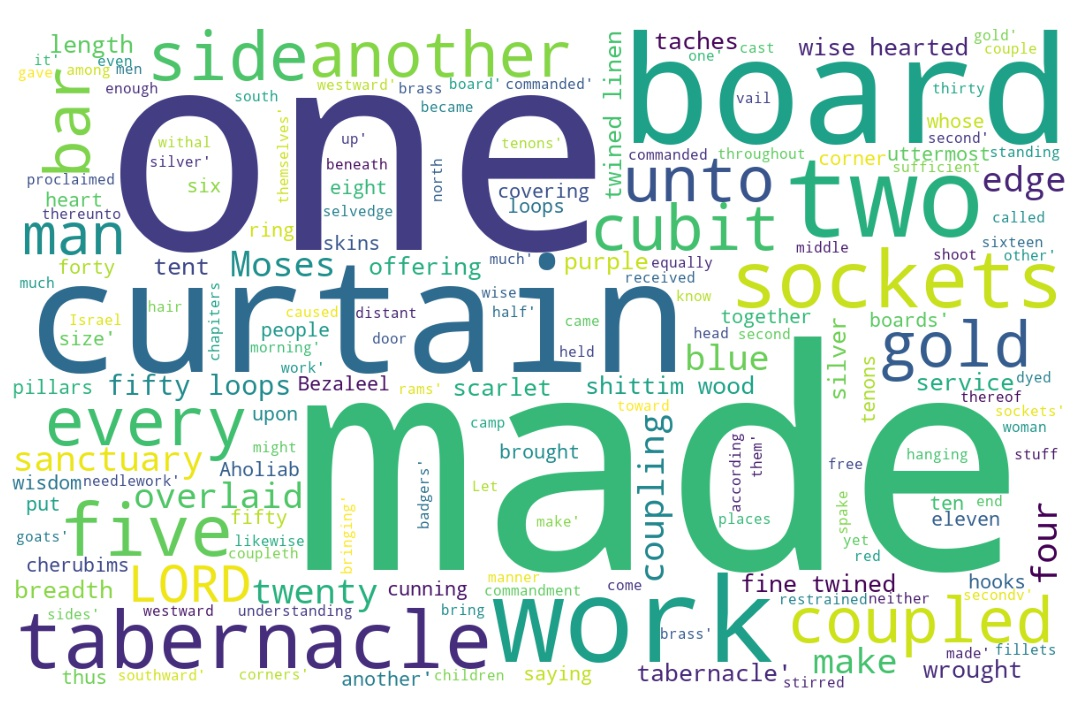
\includegraphics[width=\linewidth]{02OT-Exodus/Exodus36-WordCloud.jpg}
  \caption{Exodus 36 Word Cloud}
  \label{fig:Exodus 36 word Cloud}
\end{figure}

\marginpar{\scriptsize \centering \fcolorbox{bone}{lime}{\textbf{DOING THE WORK}}\\ (Exodus 36:1-38) \begin{compactenum}[I.][8]
    \item An \textbf{Enlightened} Group \index[scripture]{Exodus!Exo 36:01}\index[scripture]{Exodus!Exo 36:02}(Exo 36:1, 2)
    \item \textbf{Envisioned Goal} \index[scripture]{Exodus!Exo 36:02}(Exo 36:2)
    \item \textbf{Excess Giving} \index[scripture]{Exodus!Exo 36:05}(Exo 36:5)
    \item \textbf{Exhibited Grace} \index[scripture]{Exodus!Exo 36:06}(Exo 36:6) 
    \item \textbf{Echoed Guidance} \index[scripture]{Exodus!Exo 36:08-38}(Exo 36:8--38) (repeated for Exodus 26:1--37)
    \item \textbf{Employed Gold} \index[scripture]{Exodus!Exo 36:34}\index[scripture]{Exodus!Exo 36:36}(Exo 36:34, 36)
\end{compactenum}}










\footnote{\textcolor[cmyk]{0.99998,1,0,0}{\hyperlink{TOC}{Return to end of Table of Contents.}}}\footnote{\href{https://audiobible.com/bible/exodus_36.html}{\textcolor[cmyk]{0.99998,1,0,0}{Exodus 36 Audio}}}\textcolor[cmyk]{0.99998,1,0,0}{Then wrought Bezaleel and Aholiab, and every wise hearted man, in whom \fcolorbox{bone}{lime}{the LORD put wisdom and understanding} to know how to work all manner of work for the service of the sanctuary, according to all that the LORD had commanded.}
[2] \textcolor[cmyk]{0.99998,1,0,0}{And Moses called Bezaleel and Aholiab, and every wise hearted man, in whose heart the LORD \fcolorbox{bone}{lime}{had put wisdom}, \emph{even} every one whose heart \fcolorbox{bone}{lime}{stirred} him up to come unto the work to do it:}
[3] \textcolor[cmyk]{0.99998,1,0,0}{And they received of Moses all the offering, which the children of Israel had brought for the work of the service of the sanctuary, to make it \emph{withal}. And they brought yet unto him free offerings every morning.}
[4] \textcolor[cmyk]{0.99998,1,0,0}{And all the wise men, that wrought all the work of the sanctuary, came every man from his work which they made;}\\
\\
\P \textcolor[cmyk]{0.99998,1,0,0}{And they spake unto Moses, saying, The people bring much \fcolorbox{bone}{lime}{more than} \fcolorbox{bone}{lime}{enough} for the service of the work, which the LORD commanded to make.}
[6] \textcolor[cmyk]{0.99998,1,0,0}{And Moses gave commandment, and they caused it to be proclaimed throughout the camp, saying, Let neither man nor woman make any more work for the offering of the sanctuary. So the people were \fcolorbox{bone}{lime}{restrained} from bringing.}
[7] \textcolor[cmyk]{0.99998,1,0,0}{For the stuff they had was sufficient for all the work to make it, and too much.}\\
\\
\P \textcolor[cmyk]{0.99998,1,0,0}{And every wise hearted man among them that wrought the work of the \fcolorbox{bone}{bone}{tabernacle} made ten curtains \emph{of} fine twined linen, and blue, and purple, and scarlet: \emph{with} cherubims of cunning work made he them.}
[9] \textcolor[cmyk]{0.99998,1,0,0}{The length of one curtain \emph{was} twenty and eight cubits, and the breadth of one curtain four cubits: the curtains \emph{were} all of one size.}
[10] \textcolor[cmyk]{0.99998,1,0,0}{And he coupled the five curtains one unto another: and \emph{the} \emph{other} five curtains he coupled one unto another.}
[11] \textcolor[cmyk]{0.99998,1,0,0}{\fcolorbox{bone}{bone}{And he made} loops of blue on the edge of one curtain from the selvedge in the coupling: likewise he made in the uttermost side of \emph{another} curtain, in the coupling of the second.}
[12] \textcolor[cmyk]{0.99998,1,0,0}{Fifty loops made he in one curtain, and fifty loops made he in the edge of the curtain which \emph{was} in the coupling of the second: the loops held one \emph{curtain} to another.}
[13] \textcolor[cmyk]{0.99998,1,0,0}{\fcolorbox{bone}{bone}{And he made} fifty taches of gold, and coupled the curtains one unto another with the taches: so it became one \fcolorbox{bone}{bone}{tabernacle}.}\\
\\
\P \textcolor[cmyk]{0.99998,1,0,0}{\fcolorbox{bone}{bone}{And he made} curtains \emph{of} goats' \emph{hair} for the tent over the \fcolorbox{bone}{bone}{tabernacle}: eleven curtains he made them.}
[15] \textcolor[cmyk]{0.99998,1,0,0}{The length of one curtain \emph{was} thirty cubits, and four cubits \emph{was} the breadth of one curtain: the eleven curtains \emph{were} of one size.}
[16] \textcolor[cmyk]{0.99998,1,0,0}{And he coupled five curtains by themselves, and six curtains by themselves.}
[17] \textcolor[cmyk]{0.99998,1,0,0}{\fcolorbox{bone}{bone}{And he made} fifty loops upon the uttermost edge of the curtain in the coupling, and fifty loops made he upon the edge of the curtain which coupleth the second.}
[18] \textcolor[cmyk]{0.99998,1,0,0}{\fcolorbox{bone}{bone}{And he made} fifty taches \emph{of} brass to couple the tent together, that it might be one.}
[19] \textcolor[cmyk]{0.99998,1,0,0}{\fcolorbox{bone}{bone}{And he made} a covering for the tent \emph{of} rams' skins dyed red, and a covering \emph{of} badgers' skins above \emph{that}.}\\
\\
\P \textcolor[cmyk]{0.99998,1,0,0}{\fcolorbox{bone}{bone}{And he made} boards for the \fcolorbox{bone}{bone}{tabernacle} \emph{of} shittim wood, standing up.}
[21] \textcolor[cmyk]{0.99998,1,0,0}{The length of a board \emph{was} ten cubits, and the breadth of a board one cubit and a half.}
[22] \textcolor[cmyk]{0.99998,1,0,0}{One board had two tenons, equally distant one from another: thus did he make for all the boards of the \fcolorbox{bone}{bone}{tabernacle}.}
[23] \textcolor[cmyk]{0.99998,1,0,0}{\fcolorbox{bone}{bone}{And he made} boards for the \fcolorbox{bone}{bone}{tabernacle}; twenty boards for the south side southward:}
[24] \textcolor[cmyk]{0.99998,1,0,0}{And forty sockets of silver he made under the twenty boards; two sockets under one board for his two tenons, and two sockets under another board for his two tenons.}
[25] \textcolor[cmyk]{0.99998,1,0,0}{And for the other side of the \fcolorbox{bone}{bone}{tabernacle}, \emph{which} \emph{is} toward the north corner, he made twenty boards,}
[26] \textcolor[cmyk]{0.99998,1,0,0}{And their forty sockets of silver; two sockets under one board, and two sockets under another board.}
[27] \textcolor[cmyk]{0.99998,1,0,0}{And for the sides of the \fcolorbox{bone}{bone}{tabernacle} westward he made six boards.}
[28] \textcolor[cmyk]{0.99998,1,0,0}{And two boards made he for the corners of the \fcolorbox{bone}{bone}{tabernacle} in the two sides.}
[29] \textcolor[cmyk]{0.99998,1,0,0}{And they were coupled beneath, and coupled together at the head thereof, to one ring: thus he did to both of them in both the corners.}
[30] \textcolor[cmyk]{0.99998,1,0,0}{And there were eight boards; and their sockets \emph{were} sixteen sockets of silver, under every board two sockets.}\\
\\
\P \textcolor[cmyk]{0.99998,1,0,0}{\fcolorbox{bone}{bone}{And he made} bars of shittim wood; five for the boards of the one side of the \fcolorbox{bone}{bone}{tabernacle},}
[32] \textcolor[cmyk]{0.99998,1,0,0}{And five bars for the boards of the other side of the \fcolorbox{bone}{bone}{tabernacle}, and five bars for the boards of the \fcolorbox{bone}{bone}{tabernacle} for the sides westward.}
[33] \textcolor[cmyk]{0.99998,1,0,0}{\fcolorbox{bone}{bone}{And he made} the middle bar to shoot through the boards from the one end to the other.}
[34] \textcolor[cmyk]{0.99998,1,0,0}{And he overlaid the boards with \fcolorbox{bone}{lime}{gold}, and made their rings \emph{of} gold \emph{to} \emph{be} places for the bars, and overlaid the bars with \fcolorbox{bone}{lime}{gold}.}\\
\\
\P \textcolor[cmyk]{0.99998,1,0,0}{\fcolorbox{bone}{bone}{And he made} a vail \emph{of} blue, and purple, and scarlet, and fine twined linen: \emph{with} cherubims made he it of cunning work.}
[36] \textcolor[cmyk]{0.99998,1,0,0}{\fcolorbox{bone}{bone}{And he made} thereunto four pillars \emph{of} shittim \emph{wood}, and overlaid them with gold: their hooks \emph{were} \emph{of} \fcolorbox{bone}{lime}{gold}; and he cast for them four sockets of silver.}\\
\\
\P \textcolor[cmyk]{0.99998,1,0,0}{\fcolorbox{bone}{bone}{And he made} an hanging for the \fcolorbox{bone}{bone}{tabernacle} door \emph{of} blue, and purple, and scarlet, and fine twined linen, of needlework;}
[38] \textcolor[cmyk]{0.99998,1,0,0}{And the five pillars of it with their hooks: and he overlaid their chapiters and their fillets with gold: but their five sockets \emph{were} \emph{of} brass.}
\index[NWIV]{41!Exodus!Exo 36:1}\index[AWIP]{Then!Exodus!Exo 36:1}\index[AWIP]{wrought!Exodus!Exo 36:1}\index[AWIP]{Bezaleel!Exodus!Exo 36:1}\index[AWIP]{and!Exodus!Exo 36:1}\index[AWIP]{and!Exodus!Exo 36:1 (2)}\index[AWIP]{and!Exodus!Exo 36:1 (3)}\index[AWIP]{Aholiab!Exodus!Exo 36:1}\index[AWIP]{every!Exodus!Exo 36:1}\index[AWIP]{wise!Exodus!Exo 36:1}\index[AWIP]{hearted!Exodus!Exo 36:1}\index[AWIP]{man!Exodus!Exo 36:1}\index[AWIP]{in!Exodus!Exo 36:1}\index[AWIP]{whom!Exodus!Exo 36:1}\index[AWIP]{the!Exodus!Exo 36:1}\index[AWIP]{the!Exodus!Exo 36:1 (2)}\index[AWIP]{the!Exodus!Exo 36:1 (3)}\index[AWIP]{the!Exodus!Exo 36:1 (4)}\index[AWIP]{LORD!Exodus!Exo 36:1}\index[AWIP]{LORD!Exodus!Exo 36:1 (2)}\index[AWIP]{put!Exodus!Exo 36:1}\index[AWIP]{wisdom!Exodus!Exo 36:1}\index[AWIP]{understanding!Exodus!Exo 36:1}\index[AWIP]{to!Exodus!Exo 36:1}\index[AWIP]{to!Exodus!Exo 36:1 (2)}\index[AWIP]{to!Exodus!Exo 36:1 (3)}\index[AWIP]{know!Exodus!Exo 36:1}\index[AWIP]{how!Exodus!Exo 36:1}\index[AWIP]{work!Exodus!Exo 36:1}\index[AWIP]{work!Exodus!Exo 36:1 (2)}\index[AWIP]{all!Exodus!Exo 36:1}\index[AWIP]{all!Exodus!Exo 36:1 (2)}\index[AWIP]{manner!Exodus!Exo 36:1}\index[AWIP]{of!Exodus!Exo 36:1}\index[AWIP]{of!Exodus!Exo 36:1 (2)}\index[AWIP]{for!Exodus!Exo 36:1}\index[AWIP]{service!Exodus!Exo 36:1}\index[AWIP]{sanctuary!Exodus!Exo 36:1}\index[AWIP]{according!Exodus!Exo 36:1}\index[AWIP]{that!Exodus!Exo 36:1}\index[AWIP]{had!Exodus!Exo 36:1}\index[AWIP]{commanded!Exodus!Exo 36:1}

\index[NWIV]{35!Exodus!Exo 36:2}\index[AWIP]{And!Exodus!Exo 36:2}\index[AWIP]{Moses!Exodus!Exo 36:2}\index[AWIP]{called!Exodus!Exo 36:2}\index[AWIP]{Bezaleel!Exodus!Exo 36:2}\index[AWIP]{and!Exodus!Exo 36:2}\index[AWIP]{and!Exodus!Exo 36:2 (2)}\index[AWIP]{Aholiab!Exodus!Exo 36:2}\index[AWIP]{every!Exodus!Exo 36:2}\index[AWIP]{every!Exodus!Exo 36:2 (2)}\index[AWIP]{wise!Exodus!Exo 36:2}\index[AWIP]{hearted!Exodus!Exo 36:2}\index[AWIP]{man!Exodus!Exo 36:2}\index[AWIP]{in!Exodus!Exo 36:2}\index[AWIP]{whose!Exodus!Exo 36:2}\index[AWIP]{whose!Exodus!Exo 36:2 (2)}\index[AWIP]{heart!Exodus!Exo 36:2}\index[AWIP]{heart!Exodus!Exo 36:2 (2)}\index[AWIP]{the!Exodus!Exo 36:2}\index[AWIP]{the!Exodus!Exo 36:2 (2)}\index[AWIP]{LORD!Exodus!Exo 36:2}\index[AWIP]{had!Exodus!Exo 36:2}\index[AWIP]{put!Exodus!Exo 36:2}\index[AWIP]{wisdom!Exodus!Exo 36:2}\index[AWIP]{\emph{even}!Exodus!Exo 36:2}\index[AWIP]{one!Exodus!Exo 36:2}\index[AWIP]{stirred!Exodus!Exo 36:2}\index[AWIP]{him!Exodus!Exo 36:2}\index[AWIP]{up!Exodus!Exo 36:2}\index[AWIP]{to!Exodus!Exo 36:2}\index[AWIP]{to!Exodus!Exo 36:2 (2)}\index[AWIP]{come!Exodus!Exo 36:2}\index[AWIP]{unto!Exodus!Exo 36:2}\index[AWIP]{work!Exodus!Exo 36:2}\index[AWIP]{do!Exodus!Exo 36:2}\index[AWIP]{it!Exodus!Exo 36:2}\index[AWIP]{\emph{even}!Exodus!Exo 36:2}

\index[NWIV]{38!Exodus!Exo 36:3}\index[AWIP]{And!Exodus!Exo 36:3}\index[AWIP]{And!Exodus!Exo 36:3 (2)}\index[AWIP]{they!Exodus!Exo 36:3}\index[AWIP]{they!Exodus!Exo 36:3 (2)}\index[AWIP]{received!Exodus!Exo 36:3}\index[AWIP]{of!Exodus!Exo 36:3}\index[AWIP]{of!Exodus!Exo 36:3 (2)}\index[AWIP]{of!Exodus!Exo 36:3 (3)}\index[AWIP]{of!Exodus!Exo 36:3 (4)}\index[AWIP]{Moses!Exodus!Exo 36:3}\index[AWIP]{all!Exodus!Exo 36:3}\index[AWIP]{the!Exodus!Exo 36:3}\index[AWIP]{the!Exodus!Exo 36:3 (2)}\index[AWIP]{the!Exodus!Exo 36:3 (3)}\index[AWIP]{the!Exodus!Exo 36:3 (4)}\index[AWIP]{the!Exodus!Exo 36:3 (5)}\index[AWIP]{offering!Exodus!Exo 36:3}\index[AWIP]{which!Exodus!Exo 36:3}\index[AWIP]{children!Exodus!Exo 36:3}\index[AWIP]{Israel!Exodus!Exo 36:3}\index[AWIP]{had!Exodus!Exo 36:3}\index[AWIP]{brought!Exodus!Exo 36:3}\index[AWIP]{brought!Exodus!Exo 36:3 (2)}\index[AWIP]{for!Exodus!Exo 36:3}\index[AWIP]{work!Exodus!Exo 36:3}\index[AWIP]{service!Exodus!Exo 36:3}\index[AWIP]{sanctuary!Exodus!Exo 36:3}\index[AWIP]{to!Exodus!Exo 36:3}\index[AWIP]{make!Exodus!Exo 36:3}\index[AWIP]{it!Exodus!Exo 36:3}\index[AWIP]{\emph{withal}!Exodus!Exo 36:3}\index[AWIP]{yet!Exodus!Exo 36:3}\index[AWIP]{unto!Exodus!Exo 36:3}\index[AWIP]{him!Exodus!Exo 36:3}\index[AWIP]{free!Exodus!Exo 36:3}\index[AWIP]{offerings!Exodus!Exo 36:3}\index[AWIP]{every!Exodus!Exo 36:3}\index[AWIP]{morning!Exodus!Exo 36:3}\index[AWIP]{\emph{withal}!Exodus!Exo 36:3}

\index[NWIV]{22!Exodus!Exo 36:4}\index[AWIP]{And!Exodus!Exo 36:4}\index[AWIP]{all!Exodus!Exo 36:4}\index[AWIP]{all!Exodus!Exo 36:4 (2)}\index[AWIP]{the!Exodus!Exo 36:4}\index[AWIP]{the!Exodus!Exo 36:4 (2)}\index[AWIP]{the!Exodus!Exo 36:4 (3)}\index[AWIP]{wise!Exodus!Exo 36:4}\index[AWIP]{men!Exodus!Exo 36:4}\index[AWIP]{that!Exodus!Exo 36:4}\index[AWIP]{wrought!Exodus!Exo 36:4}\index[AWIP]{work!Exodus!Exo 36:4}\index[AWIP]{work!Exodus!Exo 36:4 (2)}\index[AWIP]{of!Exodus!Exo 36:4}\index[AWIP]{sanctuary!Exodus!Exo 36:4}\index[AWIP]{came!Exodus!Exo 36:4}\index[AWIP]{every!Exodus!Exo 36:4}\index[AWIP]{man!Exodus!Exo 36:4}\index[AWIP]{from!Exodus!Exo 36:4}\index[AWIP]{his!Exodus!Exo 36:4}\index[AWIP]{which!Exodus!Exo 36:4}\index[AWIP]{they!Exodus!Exo 36:4}\index[AWIP]{made!Exodus!Exo 36:4}

\index[NWIV]{25!Exodus!Exo 36:5}\index[AWIP]{And!Exodus!Exo 36:5}\index[AWIP]{they!Exodus!Exo 36:5}\index[AWIP]{spake!Exodus!Exo 36:5}\index[AWIP]{unto!Exodus!Exo 36:5}\index[AWIP]{Moses!Exodus!Exo 36:5}\index[AWIP]{saying!Exodus!Exo 36:5}\index[AWIP]{The!Exodus!Exo 36:5}\index[AWIP]{people!Exodus!Exo 36:5}\index[AWIP]{bring!Exodus!Exo 36:5}\index[AWIP]{much!Exodus!Exo 36:5}\index[AWIP]{more!Exodus!Exo 36:5}\index[AWIP]{than!Exodus!Exo 36:5}\index[AWIP]{enough!Exodus!Exo 36:5}\index[AWIP]{for!Exodus!Exo 36:5}\index[AWIP]{the!Exodus!Exo 36:5}\index[AWIP]{the!Exodus!Exo 36:5 (2)}\index[AWIP]{the!Exodus!Exo 36:5 (3)}\index[AWIP]{service!Exodus!Exo 36:5}\index[AWIP]{of!Exodus!Exo 36:5}\index[AWIP]{work!Exodus!Exo 36:5}\index[AWIP]{which!Exodus!Exo 36:5}\index[AWIP]{LORD!Exodus!Exo 36:5}\index[AWIP]{commanded!Exodus!Exo 36:5}\index[AWIP]{to!Exodus!Exo 36:5}\index[AWIP]{make!Exodus!Exo 36:5}

\index[NWIV]{37!Exodus!Exo 36:6}\index[AWIP]{And!Exodus!Exo 36:6}\index[AWIP]{Moses!Exodus!Exo 36:6}\index[AWIP]{gave!Exodus!Exo 36:6}\index[AWIP]{commandment!Exodus!Exo 36:6}\index[AWIP]{and!Exodus!Exo 36:6}\index[AWIP]{they!Exodus!Exo 36:6}\index[AWIP]{caused!Exodus!Exo 36:6}\index[AWIP]{it!Exodus!Exo 36:6}\index[AWIP]{to!Exodus!Exo 36:6}\index[AWIP]{be!Exodus!Exo 36:6}\index[AWIP]{proclaimed!Exodus!Exo 36:6}\index[AWIP]{throughout!Exodus!Exo 36:6}\index[AWIP]{the!Exodus!Exo 36:6}\index[AWIP]{the!Exodus!Exo 36:6 (2)}\index[AWIP]{the!Exodus!Exo 36:6 (3)}\index[AWIP]{the!Exodus!Exo 36:6 (4)}\index[AWIP]{camp!Exodus!Exo 36:6}\index[AWIP]{saying!Exodus!Exo 36:6}\index[AWIP]{Let!Exodus!Exo 36:6}\index[AWIP]{neither!Exodus!Exo 36:6}\index[AWIP]{man!Exodus!Exo 36:6}\index[AWIP]{nor!Exodus!Exo 36:6}\index[AWIP]{woman!Exodus!Exo 36:6}\index[AWIP]{make!Exodus!Exo 36:6}\index[AWIP]{any!Exodus!Exo 36:6}\index[AWIP]{more!Exodus!Exo 36:6}\index[AWIP]{work!Exodus!Exo 36:6}\index[AWIP]{for!Exodus!Exo 36:6}\index[AWIP]{offering!Exodus!Exo 36:6}\index[AWIP]{of!Exodus!Exo 36:6}\index[AWIP]{sanctuary!Exodus!Exo 36:6}\index[AWIP]{So!Exodus!Exo 36:6}\index[AWIP]{people!Exodus!Exo 36:6}\index[AWIP]{were!Exodus!Exo 36:6}\index[AWIP]{restrained!Exodus!Exo 36:6}\index[AWIP]{from!Exodus!Exo 36:6}\index[AWIP]{bringing!Exodus!Exo 36:6}

\index[NWIV]{17!Exodus!Exo 36:7}\index[AWIP]{For!Exodus!Exo 36:7}\index[AWIP]{the!Exodus!Exo 36:7}\index[AWIP]{the!Exodus!Exo 36:7 (2)}\index[AWIP]{stuff!Exodus!Exo 36:7}\index[AWIP]{they!Exodus!Exo 36:7}\index[AWIP]{had!Exodus!Exo 36:7}\index[AWIP]{was!Exodus!Exo 36:7}\index[AWIP]{sufficient!Exodus!Exo 36:7}\index[AWIP]{for!Exodus!Exo 36:7}\index[AWIP]{all!Exodus!Exo 36:7}\index[AWIP]{work!Exodus!Exo 36:7}\index[AWIP]{to!Exodus!Exo 36:7}\index[AWIP]{make!Exodus!Exo 36:7}\index[AWIP]{it!Exodus!Exo 36:7}\index[AWIP]{and!Exodus!Exo 36:7}\index[AWIP]{too!Exodus!Exo 36:7}\index[AWIP]{much!Exodus!Exo 36:7}

\index[NWIV]{35!Exodus!Exo 36:8}\index[AWIP]{And!Exodus!Exo 36:8}\index[AWIP]{every!Exodus!Exo 36:8}\index[AWIP]{wise!Exodus!Exo 36:8}\index[AWIP]{hearted!Exodus!Exo 36:8}\index[AWIP]{man!Exodus!Exo 36:8}\index[AWIP]{among!Exodus!Exo 36:8}\index[AWIP]{them!Exodus!Exo 36:8}\index[AWIP]{them!Exodus!Exo 36:8 (2)}\index[AWIP]{that!Exodus!Exo 36:8}\index[AWIP]{wrought!Exodus!Exo 36:8}\index[AWIP]{the!Exodus!Exo 36:8}\index[AWIP]{the!Exodus!Exo 36:8 (2)}\index[AWIP]{work!Exodus!Exo 36:8}\index[AWIP]{work!Exodus!Exo 36:8 (2)}\index[AWIP]{of!Exodus!Exo 36:8}\index[AWIP]{of!Exodus!Exo 36:8 (2)}\index[AWIP]{tabernacle!Exodus!Exo 36:8}\index[AWIP]{made!Exodus!Exo 36:8}\index[AWIP]{made!Exodus!Exo 36:8 (2)}\index[AWIP]{ten!Exodus!Exo 36:8}\index[AWIP]{curtains!Exodus!Exo 36:8}\index[AWIP]{\emph{of}!Exodus!Exo 36:8}\index[AWIP]{fine!Exodus!Exo 36:8}\index[AWIP]{twined!Exodus!Exo 36:8}\index[AWIP]{linen!Exodus!Exo 36:8}\index[AWIP]{and!Exodus!Exo 36:8}\index[AWIP]{and!Exodus!Exo 36:8 (2)}\index[AWIP]{and!Exodus!Exo 36:8 (3)}\index[AWIP]{blue!Exodus!Exo 36:8}\index[AWIP]{purple!Exodus!Exo 36:8}\index[AWIP]{scarlet!Exodus!Exo 36:8}\index[AWIP]{\emph{with}!Exodus!Exo 36:8}\index[AWIP]{cherubims!Exodus!Exo 36:8}\index[AWIP]{cunning!Exodus!Exo 36:8}\index[AWIP]{he!Exodus!Exo 36:8}\index[AWIP]{\emph{of}!Exodus!Exo 36:8}\index[AWIP]{\emph{with}!Exodus!Exo 36:8}

\index[NWIV]{25!Exodus!Exo 36:9}\index[AWIP]{The!Exodus!Exo 36:9}\index[AWIP]{length!Exodus!Exo 36:9}\index[AWIP]{of!Exodus!Exo 36:9}\index[AWIP]{of!Exodus!Exo 36:9 (2)}\index[AWIP]{of!Exodus!Exo 36:9 (3)}\index[AWIP]{one!Exodus!Exo 36:9}\index[AWIP]{one!Exodus!Exo 36:9 (2)}\index[AWIP]{one!Exodus!Exo 36:9 (3)}\index[AWIP]{curtain!Exodus!Exo 36:9}\index[AWIP]{curtain!Exodus!Exo 36:9 (2)}\index[AWIP]{\emph{was}!Exodus!Exo 36:9}\index[AWIP]{twenty!Exodus!Exo 36:9}\index[AWIP]{and!Exodus!Exo 36:9}\index[AWIP]{and!Exodus!Exo 36:9 (2)}\index[AWIP]{eight!Exodus!Exo 36:9}\index[AWIP]{cubits!Exodus!Exo 36:9}\index[AWIP]{cubits!Exodus!Exo 36:9 (2)}\index[AWIP]{the!Exodus!Exo 36:9}\index[AWIP]{the!Exodus!Exo 36:9 (2)}\index[AWIP]{breadth!Exodus!Exo 36:9}\index[AWIP]{four!Exodus!Exo 36:9}\index[AWIP]{curtains!Exodus!Exo 36:9}\index[AWIP]{\emph{were}!Exodus!Exo 36:9}\index[AWIP]{all!Exodus!Exo 36:9}\index[AWIP]{size!Exodus!Exo 36:9}\index[AWIP]{\emph{was}!Exodus!Exo 36:9}\index[AWIP]{\emph{were}!Exodus!Exo 36:9}

\index[NWIV]{19!Exodus!Exo 36:10}\index[AWIP]{And!Exodus!Exo 36:10}\index[AWIP]{he!Exodus!Exo 36:10}\index[AWIP]{he!Exodus!Exo 36:10 (2)}\index[AWIP]{coupled!Exodus!Exo 36:10}\index[AWIP]{coupled!Exodus!Exo 36:10 (2)}\index[AWIP]{the!Exodus!Exo 36:10}\index[AWIP]{five!Exodus!Exo 36:10}\index[AWIP]{five!Exodus!Exo 36:10 (2)}\index[AWIP]{curtains!Exodus!Exo 36:10}\index[AWIP]{curtains!Exodus!Exo 36:10 (2)}\index[AWIP]{one!Exodus!Exo 36:10}\index[AWIP]{one!Exodus!Exo 36:10 (2)}\index[AWIP]{unto!Exodus!Exo 36:10}\index[AWIP]{unto!Exodus!Exo 36:10 (2)}\index[AWIP]{another!Exodus!Exo 36:10}\index[AWIP]{another!Exodus!Exo 36:10 (2)}\index[AWIP]{and!Exodus!Exo 36:10}\index[AWIP]{\emph{the}!Exodus!Exo 36:10}\index[AWIP]{\emph{other}!Exodus!Exo 36:10}\index[AWIP]{\emph{the}!Exodus!Exo 36:10}\index[AWIP]{\emph{other}!Exodus!Exo 36:10}

\index[NWIV]{34!Exodus!Exo 36:11}\index[AWIP]{And!Exodus!Exo 36:11}\index[AWIP]{he!Exodus!Exo 36:11}\index[AWIP]{he!Exodus!Exo 36:11 (2)}\index[AWIP]{made!Exodus!Exo 36:11}\index[AWIP]{made!Exodus!Exo 36:11 (2)}\index[AWIP]{loops!Exodus!Exo 36:11}\index[AWIP]{of!Exodus!Exo 36:11}\index[AWIP]{of!Exodus!Exo 36:11 (2)}\index[AWIP]{of!Exodus!Exo 36:11 (3)}\index[AWIP]{of!Exodus!Exo 36:11 (4)}\index[AWIP]{blue!Exodus!Exo 36:11}\index[AWIP]{on!Exodus!Exo 36:11}\index[AWIP]{the!Exodus!Exo 36:11}\index[AWIP]{the!Exodus!Exo 36:11 (2)}\index[AWIP]{the!Exodus!Exo 36:11 (3)}\index[AWIP]{the!Exodus!Exo 36:11 (4)}\index[AWIP]{the!Exodus!Exo 36:11 (5)}\index[AWIP]{the!Exodus!Exo 36:11 (6)}\index[AWIP]{edge!Exodus!Exo 36:11}\index[AWIP]{one!Exodus!Exo 36:11}\index[AWIP]{curtain!Exodus!Exo 36:11}\index[AWIP]{curtain!Exodus!Exo 36:11 (2)}\index[AWIP]{from!Exodus!Exo 36:11}\index[AWIP]{selvedge!Exodus!Exo 36:11}\index[AWIP]{in!Exodus!Exo 36:11}\index[AWIP]{in!Exodus!Exo 36:11 (2)}\index[AWIP]{in!Exodus!Exo 36:11 (3)}\index[AWIP]{coupling!Exodus!Exo 36:11}\index[AWIP]{coupling!Exodus!Exo 36:11 (2)}\index[AWIP]{likewise!Exodus!Exo 36:11}\index[AWIP]{uttermost!Exodus!Exo 36:11}\index[AWIP]{side!Exodus!Exo 36:11}\index[AWIP]{\emph{another}!Exodus!Exo 36:11}\index[AWIP]{second!Exodus!Exo 36:11}\index[AWIP]{\emph{another}!Exodus!Exo 36:11}

\index[NWIV]{33!Exodus!Exo 36:12}\index[AWIP]{Fifty!Exodus!Exo 36:12}\index[AWIP]{loops!Exodus!Exo 36:12}\index[AWIP]{loops!Exodus!Exo 36:12 (2)}\index[AWIP]{loops!Exodus!Exo 36:12 (3)}\index[AWIP]{made!Exodus!Exo 36:12}\index[AWIP]{made!Exodus!Exo 36:12 (2)}\index[AWIP]{he!Exodus!Exo 36:12}\index[AWIP]{he!Exodus!Exo 36:12 (2)}\index[AWIP]{in!Exodus!Exo 36:12}\index[AWIP]{in!Exodus!Exo 36:12 (2)}\index[AWIP]{in!Exodus!Exo 36:12 (3)}\index[AWIP]{one!Exodus!Exo 36:12}\index[AWIP]{one!Exodus!Exo 36:12 (2)}\index[AWIP]{curtain!Exodus!Exo 36:12}\index[AWIP]{curtain!Exodus!Exo 36:12 (2)}\index[AWIP]{and!Exodus!Exo 36:12}\index[AWIP]{fifty!Exodus!Exo 36:12}\index[AWIP]{the!Exodus!Exo 36:12}\index[AWIP]{the!Exodus!Exo 36:12 (2)}\index[AWIP]{the!Exodus!Exo 36:12 (3)}\index[AWIP]{the!Exodus!Exo 36:12 (4)}\index[AWIP]{the!Exodus!Exo 36:12 (5)}\index[AWIP]{edge!Exodus!Exo 36:12}\index[AWIP]{of!Exodus!Exo 36:12}\index[AWIP]{of!Exodus!Exo 36:12 (2)}\index[AWIP]{which!Exodus!Exo 36:12}\index[AWIP]{\emph{was}!Exodus!Exo 36:12}\index[AWIP]{coupling!Exodus!Exo 36:12}\index[AWIP]{second!Exodus!Exo 36:12}\index[AWIP]{held!Exodus!Exo 36:12}\index[AWIP]{\emph{curtain}!Exodus!Exo 36:12}\index[AWIP]{to!Exodus!Exo 36:12}\index[AWIP]{another!Exodus!Exo 36:12}\index[AWIP]{\emph{was}!Exodus!Exo 36:12}\index[AWIP]{\emph{curtain}!Exodus!Exo 36:12}

\index[NWIV]{22!Exodus!Exo 36:13}\index[AWIP]{And!Exodus!Exo 36:13}\index[AWIP]{he!Exodus!Exo 36:13}\index[AWIP]{made!Exodus!Exo 36:13}\index[AWIP]{fifty!Exodus!Exo 36:13}\index[AWIP]{taches!Exodus!Exo 36:13}\index[AWIP]{taches!Exodus!Exo 36:13 (2)}\index[AWIP]{of!Exodus!Exo 36:13}\index[AWIP]{gold!Exodus!Exo 36:13}\index[AWIP]{and!Exodus!Exo 36:13}\index[AWIP]{coupled!Exodus!Exo 36:13}\index[AWIP]{the!Exodus!Exo 36:13}\index[AWIP]{the!Exodus!Exo 36:13 (2)}\index[AWIP]{curtains!Exodus!Exo 36:13}\index[AWIP]{one!Exodus!Exo 36:13}\index[AWIP]{one!Exodus!Exo 36:13 (2)}\index[AWIP]{unto!Exodus!Exo 36:13}\index[AWIP]{another!Exodus!Exo 36:13}\index[AWIP]{with!Exodus!Exo 36:13}\index[AWIP]{so!Exodus!Exo 36:13}\index[AWIP]{it!Exodus!Exo 36:13}\index[AWIP]{became!Exodus!Exo 36:13}\index[AWIP]{tabernacle!Exodus!Exo 36:13}

\index[NWIV]{18!Exodus!Exo 36:14}\index[AWIP]{And!Exodus!Exo 36:14}\index[AWIP]{he!Exodus!Exo 36:14}\index[AWIP]{he!Exodus!Exo 36:14 (2)}\index[AWIP]{made!Exodus!Exo 36:14}\index[AWIP]{made!Exodus!Exo 36:14 (2)}\index[AWIP]{curtains!Exodus!Exo 36:14}\index[AWIP]{curtains!Exodus!Exo 36:14 (2)}\index[AWIP]{\emph{of}!Exodus!Exo 36:14}\index[AWIP]{goats'!Exodus!Exo 36:14}\index[AWIP]{\emph{hair}!Exodus!Exo 36:14}\index[AWIP]{for!Exodus!Exo 36:14}\index[AWIP]{the!Exodus!Exo 36:14}\index[AWIP]{the!Exodus!Exo 36:14 (2)}\index[AWIP]{tent!Exodus!Exo 36:14}\index[AWIP]{over!Exodus!Exo 36:14}\index[AWIP]{tabernacle!Exodus!Exo 36:14}\index[AWIP]{eleven!Exodus!Exo 36:14}\index[AWIP]{them!Exodus!Exo 36:14}\index[AWIP]{\emph{of}!Exodus!Exo 36:14}\index[AWIP]{\emph{hair}!Exodus!Exo 36:14}

\index[NWIV]{24!Exodus!Exo 36:15}\index[AWIP]{The!Exodus!Exo 36:15}\index[AWIP]{length!Exodus!Exo 36:15}\index[AWIP]{of!Exodus!Exo 36:15}\index[AWIP]{of!Exodus!Exo 36:15 (2)}\index[AWIP]{of!Exodus!Exo 36:15 (3)}\index[AWIP]{one!Exodus!Exo 36:15}\index[AWIP]{one!Exodus!Exo 36:15 (2)}\index[AWIP]{one!Exodus!Exo 36:15 (3)}\index[AWIP]{curtain!Exodus!Exo 36:15}\index[AWIP]{curtain!Exodus!Exo 36:15 (2)}\index[AWIP]{\emph{was}!Exodus!Exo 36:15}\index[AWIP]{\emph{was}!Exodus!Exo 36:15 (2)}\index[AWIP]{thirty!Exodus!Exo 36:15}\index[AWIP]{cubits!Exodus!Exo 36:15}\index[AWIP]{cubits!Exodus!Exo 36:15 (2)}\index[AWIP]{and!Exodus!Exo 36:15}\index[AWIP]{four!Exodus!Exo 36:15}\index[AWIP]{the!Exodus!Exo 36:15}\index[AWIP]{the!Exodus!Exo 36:15 (2)}\index[AWIP]{breadth!Exodus!Exo 36:15}\index[AWIP]{eleven!Exodus!Exo 36:15}\index[AWIP]{curtains!Exodus!Exo 36:15}\index[AWIP]{\emph{were}!Exodus!Exo 36:15}\index[AWIP]{size!Exodus!Exo 36:15}\index[AWIP]{\emph{was}!Exodus!Exo 36:15}\index[AWIP]{\emph{was}!Exodus!Exo 36:15 (2)}\index[AWIP]{\emph{were}!Exodus!Exo 36:15}

\index[NWIV]{12!Exodus!Exo 36:16}\index[AWIP]{And!Exodus!Exo 36:16}\index[AWIP]{he!Exodus!Exo 36:16}\index[AWIP]{coupled!Exodus!Exo 36:16}\index[AWIP]{five!Exodus!Exo 36:16}\index[AWIP]{curtains!Exodus!Exo 36:16}\index[AWIP]{curtains!Exodus!Exo 36:16 (2)}\index[AWIP]{by!Exodus!Exo 36:16}\index[AWIP]{by!Exodus!Exo 36:16 (2)}\index[AWIP]{themselves!Exodus!Exo 36:16}\index[AWIP]{themselves!Exodus!Exo 36:16 (2)}\index[AWIP]{and!Exodus!Exo 36:16}\index[AWIP]{six!Exodus!Exo 36:16}

\index[NWIV]{30!Exodus!Exo 36:17}\index[AWIP]{And!Exodus!Exo 36:17}\index[AWIP]{he!Exodus!Exo 36:17}\index[AWIP]{he!Exodus!Exo 36:17 (2)}\index[AWIP]{made!Exodus!Exo 36:17}\index[AWIP]{made!Exodus!Exo 36:17 (2)}\index[AWIP]{fifty!Exodus!Exo 36:17}\index[AWIP]{fifty!Exodus!Exo 36:17 (2)}\index[AWIP]{loops!Exodus!Exo 36:17}\index[AWIP]{loops!Exodus!Exo 36:17 (2)}\index[AWIP]{upon!Exodus!Exo 36:17}\index[AWIP]{upon!Exodus!Exo 36:17 (2)}\index[AWIP]{the!Exodus!Exo 36:17}\index[AWIP]{the!Exodus!Exo 36:17 (2)}\index[AWIP]{the!Exodus!Exo 36:17 (3)}\index[AWIP]{the!Exodus!Exo 36:17 (4)}\index[AWIP]{the!Exodus!Exo 36:17 (5)}\index[AWIP]{the!Exodus!Exo 36:17 (6)}\index[AWIP]{uttermost!Exodus!Exo 36:17}\index[AWIP]{edge!Exodus!Exo 36:17}\index[AWIP]{edge!Exodus!Exo 36:17 (2)}\index[AWIP]{of!Exodus!Exo 36:17}\index[AWIP]{of!Exodus!Exo 36:17 (2)}\index[AWIP]{curtain!Exodus!Exo 36:17}\index[AWIP]{curtain!Exodus!Exo 36:17 (2)}\index[AWIP]{in!Exodus!Exo 36:17}\index[AWIP]{coupling!Exodus!Exo 36:17}\index[AWIP]{and!Exodus!Exo 36:17}\index[AWIP]{which!Exodus!Exo 36:17}\index[AWIP]{coupleth!Exodus!Exo 36:17}\index[AWIP]{secondv!Exodus!Exo 36:17}

\index[NWIV]{17!Exodus!Exo 36:18}\index[AWIP]{And!Exodus!Exo 36:18}\index[AWIP]{he!Exodus!Exo 36:18}\index[AWIP]{made!Exodus!Exo 36:18}\index[AWIP]{fifty!Exodus!Exo 36:18}\index[AWIP]{taches!Exodus!Exo 36:18}\index[AWIP]{\emph{of}!Exodus!Exo 36:18}\index[AWIP]{brass!Exodus!Exo 36:18}\index[AWIP]{to!Exodus!Exo 36:18}\index[AWIP]{couple!Exodus!Exo 36:18}\index[AWIP]{the!Exodus!Exo 36:18}\index[AWIP]{tent!Exodus!Exo 36:18}\index[AWIP]{together!Exodus!Exo 36:18}\index[AWIP]{that!Exodus!Exo 36:18}\index[AWIP]{it!Exodus!Exo 36:18}\index[AWIP]{might!Exodus!Exo 36:18}\index[AWIP]{be!Exodus!Exo 36:18}\index[AWIP]{one!Exodus!Exo 36:18}\index[AWIP]{\emph{of}!Exodus!Exo 36:18}

\index[NWIV]{21!Exodus!Exo 36:19}\index[AWIP]{And!Exodus!Exo 36:19}\index[AWIP]{he!Exodus!Exo 36:19}\index[AWIP]{made!Exodus!Exo 36:19}\index[AWIP]{a!Exodus!Exo 36:19}\index[AWIP]{a!Exodus!Exo 36:19 (2)}\index[AWIP]{covering!Exodus!Exo 36:19}\index[AWIP]{covering!Exodus!Exo 36:19 (2)}\index[AWIP]{for!Exodus!Exo 36:19}\index[AWIP]{the!Exodus!Exo 36:19}\index[AWIP]{tent!Exodus!Exo 36:19}\index[AWIP]{\emph{of}!Exodus!Exo 36:19}\index[AWIP]{\emph{of}!Exodus!Exo 36:19 (2)}\index[AWIP]{rams'!Exodus!Exo 36:19}\index[AWIP]{skins!Exodus!Exo 36:19}\index[AWIP]{skins!Exodus!Exo 36:19 (2)}\index[AWIP]{dyed!Exodus!Exo 36:19}\index[AWIP]{red!Exodus!Exo 36:19}\index[AWIP]{and!Exodus!Exo 36:19}\index[AWIP]{badgers'!Exodus!Exo 36:19}\index[AWIP]{above!Exodus!Exo 36:19}\index[AWIP]{\emph{that}!Exodus!Exo 36:19}\index[AWIP]{\emph{of}!Exodus!Exo 36:19}\index[AWIP]{\emph{of}!Exodus!Exo 36:19 (2)}\index[AWIP]{\emph{that}!Exodus!Exo 36:19}

\index[NWIV]{12!Exodus!Exo 36:20}\index[AWIP]{And!Exodus!Exo 36:20}\index[AWIP]{he!Exodus!Exo 36:20}\index[AWIP]{made!Exodus!Exo 36:20}\index[AWIP]{boards!Exodus!Exo 36:20}\index[AWIP]{for!Exodus!Exo 36:20}\index[AWIP]{the!Exodus!Exo 36:20}\index[AWIP]{tabernacle!Exodus!Exo 36:20}\index[AWIP]{\emph{of}!Exodus!Exo 36:20}\index[AWIP]{shittim!Exodus!Exo 36:20}\index[AWIP]{wood!Exodus!Exo 36:20}\index[AWIP]{standing!Exodus!Exo 36:20}\index[AWIP]{up!Exodus!Exo 36:20}\index[AWIP]{\emph{of}!Exodus!Exo 36:20}

\index[NWIV]{19!Exodus!Exo 36:21}\index[AWIP]{The!Exodus!Exo 36:21}\index[AWIP]{length!Exodus!Exo 36:21}\index[AWIP]{of!Exodus!Exo 36:21}\index[AWIP]{of!Exodus!Exo 36:21 (2)}\index[AWIP]{a!Exodus!Exo 36:21}\index[AWIP]{a!Exodus!Exo 36:21 (2)}\index[AWIP]{a!Exodus!Exo 36:21 (3)}\index[AWIP]{board!Exodus!Exo 36:21}\index[AWIP]{board!Exodus!Exo 36:21 (2)}\index[AWIP]{\emph{was}!Exodus!Exo 36:21}\index[AWIP]{ten!Exodus!Exo 36:21}\index[AWIP]{cubits!Exodus!Exo 36:21}\index[AWIP]{and!Exodus!Exo 36:21}\index[AWIP]{and!Exodus!Exo 36:21 (2)}\index[AWIP]{the!Exodus!Exo 36:21}\index[AWIP]{breadth!Exodus!Exo 36:21}\index[AWIP]{one!Exodus!Exo 36:21}\index[AWIP]{cubit!Exodus!Exo 36:21}\index[AWIP]{half!Exodus!Exo 36:21}\index[AWIP]{\emph{was}!Exodus!Exo 36:21}

\index[NWIV]{21!Exodus!Exo 36:22}\index[AWIP]{One!Exodus!Exo 36:22}\index[AWIP]{board!Exodus!Exo 36:22}\index[AWIP]{had!Exodus!Exo 36:22}\index[AWIP]{two!Exodus!Exo 36:22}\index[AWIP]{tenons!Exodus!Exo 36:22}\index[AWIP]{equally!Exodus!Exo 36:22}\index[AWIP]{distant!Exodus!Exo 36:22}\index[AWIP]{one!Exodus!Exo 36:22}\index[AWIP]{from!Exodus!Exo 36:22}\index[AWIP]{another!Exodus!Exo 36:22}\index[AWIP]{thus!Exodus!Exo 36:22}\index[AWIP]{did!Exodus!Exo 36:22}\index[AWIP]{he!Exodus!Exo 36:22}\index[AWIP]{make!Exodus!Exo 36:22}\index[AWIP]{for!Exodus!Exo 36:22}\index[AWIP]{all!Exodus!Exo 36:22}\index[AWIP]{the!Exodus!Exo 36:22}\index[AWIP]{the!Exodus!Exo 36:22 (2)}\index[AWIP]{boards!Exodus!Exo 36:22}\index[AWIP]{of!Exodus!Exo 36:22}\index[AWIP]{tabernacle!Exodus!Exo 36:22}

\index[NWIV]{14!Exodus!Exo 36:23}\index[AWIP]{And!Exodus!Exo 36:23}\index[AWIP]{he!Exodus!Exo 36:23}\index[AWIP]{made!Exodus!Exo 36:23}\index[AWIP]{boards!Exodus!Exo 36:23}\index[AWIP]{boards!Exodus!Exo 36:23 (2)}\index[AWIP]{for!Exodus!Exo 36:23}\index[AWIP]{for!Exodus!Exo 36:23 (2)}\index[AWIP]{the!Exodus!Exo 36:23}\index[AWIP]{the!Exodus!Exo 36:23 (2)}\index[AWIP]{tabernacle!Exodus!Exo 36:23}\index[AWIP]{twenty!Exodus!Exo 36:23}\index[AWIP]{south!Exodus!Exo 36:23}\index[AWIP]{side!Exodus!Exo 36:23}\index[AWIP]{southward!Exodus!Exo 36:23}

\index[NWIV]{30!Exodus!Exo 36:24}\index[AWIP]{And!Exodus!Exo 36:24}\index[AWIP]{forty!Exodus!Exo 36:24}\index[AWIP]{sockets!Exodus!Exo 36:24}\index[AWIP]{sockets!Exodus!Exo 36:24 (2)}\index[AWIP]{sockets!Exodus!Exo 36:24 (3)}\index[AWIP]{of!Exodus!Exo 36:24}\index[AWIP]{silver!Exodus!Exo 36:24}\index[AWIP]{he!Exodus!Exo 36:24}\index[AWIP]{made!Exodus!Exo 36:24}\index[AWIP]{under!Exodus!Exo 36:24}\index[AWIP]{under!Exodus!Exo 36:24 (2)}\index[AWIP]{under!Exodus!Exo 36:24 (3)}\index[AWIP]{the!Exodus!Exo 36:24}\index[AWIP]{twenty!Exodus!Exo 36:24}\index[AWIP]{boards!Exodus!Exo 36:24}\index[AWIP]{two!Exodus!Exo 36:24}\index[AWIP]{two!Exodus!Exo 36:24 (2)}\index[AWIP]{two!Exodus!Exo 36:24 (3)}\index[AWIP]{two!Exodus!Exo 36:24 (4)}\index[AWIP]{one!Exodus!Exo 36:24}\index[AWIP]{board!Exodus!Exo 36:24}\index[AWIP]{board!Exodus!Exo 36:24 (2)}\index[AWIP]{for!Exodus!Exo 36:24}\index[AWIP]{for!Exodus!Exo 36:24 (2)}\index[AWIP]{his!Exodus!Exo 36:24}\index[AWIP]{his!Exodus!Exo 36:24 (2)}\index[AWIP]{tenons!Exodus!Exo 36:24}\index[AWIP]{tenons!Exodus!Exo 36:24 (2)}\index[AWIP]{and!Exodus!Exo 36:24}\index[AWIP]{another!Exodus!Exo 36:24}

\index[NWIV]{18!Exodus!Exo 36:25}\index[AWIP]{And!Exodus!Exo 36:25}\index[AWIP]{for!Exodus!Exo 36:25}\index[AWIP]{the!Exodus!Exo 36:25}\index[AWIP]{the!Exodus!Exo 36:25 (2)}\index[AWIP]{the!Exodus!Exo 36:25 (3)}\index[AWIP]{other!Exodus!Exo 36:25}\index[AWIP]{side!Exodus!Exo 36:25}\index[AWIP]{of!Exodus!Exo 36:25}\index[AWIP]{tabernacle!Exodus!Exo 36:25}\index[AWIP]{\emph{which}!Exodus!Exo 36:25}\index[AWIP]{\emph{is}!Exodus!Exo 36:25}\index[AWIP]{toward!Exodus!Exo 36:25}\index[AWIP]{north!Exodus!Exo 36:25}\index[AWIP]{corner!Exodus!Exo 36:25}\index[AWIP]{he!Exodus!Exo 36:25}\index[AWIP]{made!Exodus!Exo 36:25}\index[AWIP]{twenty!Exodus!Exo 36:25}\index[AWIP]{boards!Exodus!Exo 36:25}\index[AWIP]{\emph{which}!Exodus!Exo 36:25}\index[AWIP]{\emph{is}!Exodus!Exo 36:25}

\index[NWIV]{17!Exodus!Exo 36:26}\index[AWIP]{And!Exodus!Exo 36:26}\index[AWIP]{their!Exodus!Exo 36:26}\index[AWIP]{forty!Exodus!Exo 36:26}\index[AWIP]{sockets!Exodus!Exo 36:26}\index[AWIP]{sockets!Exodus!Exo 36:26 (2)}\index[AWIP]{sockets!Exodus!Exo 36:26 (3)}\index[AWIP]{of!Exodus!Exo 36:26}\index[AWIP]{silver!Exodus!Exo 36:26}\index[AWIP]{two!Exodus!Exo 36:26}\index[AWIP]{two!Exodus!Exo 36:26 (2)}\index[AWIP]{under!Exodus!Exo 36:26}\index[AWIP]{under!Exodus!Exo 36:26 (2)}\index[AWIP]{one!Exodus!Exo 36:26}\index[AWIP]{board!Exodus!Exo 36:26}\index[AWIP]{board!Exodus!Exo 36:26 (2)}\index[AWIP]{and!Exodus!Exo 36:26}\index[AWIP]{another!Exodus!Exo 36:26}

\index[NWIV]{12!Exodus!Exo 36:27}\index[AWIP]{And!Exodus!Exo 36:27}\index[AWIP]{for!Exodus!Exo 36:27}\index[AWIP]{the!Exodus!Exo 36:27}\index[AWIP]{the!Exodus!Exo 36:27 (2)}\index[AWIP]{sides!Exodus!Exo 36:27}\index[AWIP]{of!Exodus!Exo 36:27}\index[AWIP]{tabernacle!Exodus!Exo 36:27}\index[AWIP]{westward!Exodus!Exo 36:27}\index[AWIP]{he!Exodus!Exo 36:27}\index[AWIP]{made!Exodus!Exo 36:27}\index[AWIP]{six!Exodus!Exo 36:27}\index[AWIP]{boards!Exodus!Exo 36:27}

\index[NWIV]{15!Exodus!Exo 36:28}\index[AWIP]{And!Exodus!Exo 36:28}\index[AWIP]{two!Exodus!Exo 36:28}\index[AWIP]{two!Exodus!Exo 36:28 (2)}\index[AWIP]{boards!Exodus!Exo 36:28}\index[AWIP]{made!Exodus!Exo 36:28}\index[AWIP]{he!Exodus!Exo 36:28}\index[AWIP]{for!Exodus!Exo 36:28}\index[AWIP]{the!Exodus!Exo 36:28}\index[AWIP]{the!Exodus!Exo 36:28 (2)}\index[AWIP]{the!Exodus!Exo 36:28 (3)}\index[AWIP]{corners!Exodus!Exo 36:28}\index[AWIP]{of!Exodus!Exo 36:28}\index[AWIP]{tabernacle!Exodus!Exo 36:28}\index[AWIP]{in!Exodus!Exo 36:28}\index[AWIP]{sides!Exodus!Exo 36:28}

\index[NWIV]{26!Exodus!Exo 36:29}\index[AWIP]{And!Exodus!Exo 36:29}\index[AWIP]{they!Exodus!Exo 36:29}\index[AWIP]{were!Exodus!Exo 36:29}\index[AWIP]{coupled!Exodus!Exo 36:29}\index[AWIP]{coupled!Exodus!Exo 36:29 (2)}\index[AWIP]{beneath!Exodus!Exo 36:29}\index[AWIP]{and!Exodus!Exo 36:29}\index[AWIP]{together!Exodus!Exo 36:29}\index[AWIP]{at!Exodus!Exo 36:29}\index[AWIP]{the!Exodus!Exo 36:29}\index[AWIP]{the!Exodus!Exo 36:29 (2)}\index[AWIP]{head!Exodus!Exo 36:29}\index[AWIP]{thereof!Exodus!Exo 36:29}\index[AWIP]{to!Exodus!Exo 36:29}\index[AWIP]{to!Exodus!Exo 36:29 (2)}\index[AWIP]{one!Exodus!Exo 36:29}\index[AWIP]{ring!Exodus!Exo 36:29}\index[AWIP]{thus!Exodus!Exo 36:29}\index[AWIP]{he!Exodus!Exo 36:29}\index[AWIP]{did!Exodus!Exo 36:29}\index[AWIP]{both!Exodus!Exo 36:29}\index[AWIP]{both!Exodus!Exo 36:29 (2)}\index[AWIP]{of!Exodus!Exo 36:29}\index[AWIP]{them!Exodus!Exo 36:29}\index[AWIP]{in!Exodus!Exo 36:29}\index[AWIP]{corners!Exodus!Exo 36:29}

\index[NWIV]{18!Exodus!Exo 36:30}\index[AWIP]{And!Exodus!Exo 36:30}\index[AWIP]{there!Exodus!Exo 36:30}\index[AWIP]{were!Exodus!Exo 36:30}\index[AWIP]{eight!Exodus!Exo 36:30}\index[AWIP]{boards!Exodus!Exo 36:30}\index[AWIP]{and!Exodus!Exo 36:30}\index[AWIP]{their!Exodus!Exo 36:30}\index[AWIP]{sockets!Exodus!Exo 36:30}\index[AWIP]{sockets!Exodus!Exo 36:30 (2)}\index[AWIP]{sockets!Exodus!Exo 36:30 (3)}\index[AWIP]{\emph{were}!Exodus!Exo 36:30}\index[AWIP]{sixteen!Exodus!Exo 36:30}\index[AWIP]{of!Exodus!Exo 36:30}\index[AWIP]{silver!Exodus!Exo 36:30}\index[AWIP]{under!Exodus!Exo 36:30}\index[AWIP]{every!Exodus!Exo 36:30}\index[AWIP]{board!Exodus!Exo 36:30}\index[AWIP]{two!Exodus!Exo 36:30}\index[AWIP]{\emph{were}!Exodus!Exo 36:30}

\index[NWIV]{18!Exodus!Exo 36:31}\index[AWIP]{And!Exodus!Exo 36:31}\index[AWIP]{he!Exodus!Exo 36:31}\index[AWIP]{made!Exodus!Exo 36:31}\index[AWIP]{bars!Exodus!Exo 36:31}\index[AWIP]{of!Exodus!Exo 36:31}\index[AWIP]{of!Exodus!Exo 36:31 (2)}\index[AWIP]{of!Exodus!Exo 36:31 (3)}\index[AWIP]{shittim!Exodus!Exo 36:31}\index[AWIP]{wood!Exodus!Exo 36:31}\index[AWIP]{five!Exodus!Exo 36:31}\index[AWIP]{for!Exodus!Exo 36:31}\index[AWIP]{the!Exodus!Exo 36:31}\index[AWIP]{the!Exodus!Exo 36:31 (2)}\index[AWIP]{the!Exodus!Exo 36:31 (3)}\index[AWIP]{boards!Exodus!Exo 36:31}\index[AWIP]{one!Exodus!Exo 36:31}\index[AWIP]{side!Exodus!Exo 36:31}\index[AWIP]{tabernacle!Exodus!Exo 36:31}

\index[NWIV]{26!Exodus!Exo 36:32}\index[AWIP]{And!Exodus!Exo 36:32}\index[AWIP]{five!Exodus!Exo 36:32}\index[AWIP]{five!Exodus!Exo 36:32 (2)}\index[AWIP]{bars!Exodus!Exo 36:32}\index[AWIP]{bars!Exodus!Exo 36:32 (2)}\index[AWIP]{for!Exodus!Exo 36:32}\index[AWIP]{for!Exodus!Exo 36:32 (2)}\index[AWIP]{for!Exodus!Exo 36:32 (3)}\index[AWIP]{the!Exodus!Exo 36:32}\index[AWIP]{the!Exodus!Exo 36:32 (2)}\index[AWIP]{the!Exodus!Exo 36:32 (3)}\index[AWIP]{the!Exodus!Exo 36:32 (4)}\index[AWIP]{the!Exodus!Exo 36:32 (5)}\index[AWIP]{the!Exodus!Exo 36:32 (6)}\index[AWIP]{boards!Exodus!Exo 36:32}\index[AWIP]{boards!Exodus!Exo 36:32 (2)}\index[AWIP]{of!Exodus!Exo 36:32}\index[AWIP]{of!Exodus!Exo 36:32 (2)}\index[AWIP]{of!Exodus!Exo 36:32 (3)}\index[AWIP]{other!Exodus!Exo 36:32}\index[AWIP]{side!Exodus!Exo 36:32}\index[AWIP]{tabernacle!Exodus!Exo 36:32}\index[AWIP]{tabernacle!Exodus!Exo 36:32 (2)}\index[AWIP]{and!Exodus!Exo 36:32}\index[AWIP]{sides!Exodus!Exo 36:32}\index[AWIP]{westward!Exodus!Exo 36:32}

\index[NWIV]{18!Exodus!Exo 36:33}\index[AWIP]{And!Exodus!Exo 36:33}\index[AWIP]{he!Exodus!Exo 36:33}\index[AWIP]{made!Exodus!Exo 36:33}\index[AWIP]{the!Exodus!Exo 36:33}\index[AWIP]{the!Exodus!Exo 36:33 (2)}\index[AWIP]{the!Exodus!Exo 36:33 (3)}\index[AWIP]{the!Exodus!Exo 36:33 (4)}\index[AWIP]{middle!Exodus!Exo 36:33}\index[AWIP]{bar!Exodus!Exo 36:33}\index[AWIP]{to!Exodus!Exo 36:33}\index[AWIP]{to!Exodus!Exo 36:33 (2)}\index[AWIP]{shoot!Exodus!Exo 36:33}\index[AWIP]{through!Exodus!Exo 36:33}\index[AWIP]{boards!Exodus!Exo 36:33}\index[AWIP]{from!Exodus!Exo 36:33}\index[AWIP]{one!Exodus!Exo 36:33}\index[AWIP]{end!Exodus!Exo 36:33}\index[AWIP]{other!Exodus!Exo 36:33}

\index[NWIV]{25!Exodus!Exo 36:34}\index[AWIP]{And!Exodus!Exo 36:34}\index[AWIP]{he!Exodus!Exo 36:34}\index[AWIP]{overlaid!Exodus!Exo 36:34}\index[AWIP]{overlaid!Exodus!Exo 36:34 (2)}\index[AWIP]{the!Exodus!Exo 36:34}\index[AWIP]{the!Exodus!Exo 36:34 (2)}\index[AWIP]{the!Exodus!Exo 36:34 (3)}\index[AWIP]{boards!Exodus!Exo 36:34}\index[AWIP]{with!Exodus!Exo 36:34}\index[AWIP]{with!Exodus!Exo 36:34 (2)}\index[AWIP]{gold!Exodus!Exo 36:34}\index[AWIP]{gold!Exodus!Exo 36:34 (2)}\index[AWIP]{gold!Exodus!Exo 36:34 (3)}\index[AWIP]{and!Exodus!Exo 36:34}\index[AWIP]{and!Exodus!Exo 36:34 (2)}\index[AWIP]{made!Exodus!Exo 36:34}\index[AWIP]{their!Exodus!Exo 36:34}\index[AWIP]{rings!Exodus!Exo 36:34}\index[AWIP]{\emph{of}!Exodus!Exo 36:34}\index[AWIP]{\emph{to}!Exodus!Exo 36:34}\index[AWIP]{\emph{be}!Exodus!Exo 36:34}\index[AWIP]{places!Exodus!Exo 36:34}\index[AWIP]{for!Exodus!Exo 36:34}\index[AWIP]{bars!Exodus!Exo 36:34}\index[AWIP]{bars!Exodus!Exo 36:34 (2)}\index[AWIP]{\emph{of}!Exodus!Exo 36:34}\index[AWIP]{\emph{to}!Exodus!Exo 36:34}\index[AWIP]{\emph{be}!Exodus!Exo 36:34}

\index[NWIV]{23!Exodus!Exo 36:35}\index[AWIP]{And!Exodus!Exo 36:35}\index[AWIP]{he!Exodus!Exo 36:35}\index[AWIP]{he!Exodus!Exo 36:35 (2)}\index[AWIP]{made!Exodus!Exo 36:35}\index[AWIP]{made!Exodus!Exo 36:35 (2)}\index[AWIP]{a!Exodus!Exo 36:35}\index[AWIP]{vail!Exodus!Exo 36:35}\index[AWIP]{\emph{of}!Exodus!Exo 36:35}\index[AWIP]{blue!Exodus!Exo 36:35}\index[AWIP]{and!Exodus!Exo 36:35}\index[AWIP]{and!Exodus!Exo 36:35 (2)}\index[AWIP]{and!Exodus!Exo 36:35 (3)}\index[AWIP]{purple!Exodus!Exo 36:35}\index[AWIP]{scarlet!Exodus!Exo 36:35}\index[AWIP]{fine!Exodus!Exo 36:35}\index[AWIP]{twined!Exodus!Exo 36:35}\index[AWIP]{linen!Exodus!Exo 36:35}\index[AWIP]{\emph{with}!Exodus!Exo 36:35}\index[AWIP]{cherubims!Exodus!Exo 36:35}\index[AWIP]{it!Exodus!Exo 36:35}\index[AWIP]{of!Exodus!Exo 36:35}\index[AWIP]{cunning!Exodus!Exo 36:35}\index[AWIP]{work!Exodus!Exo 36:35}\index[AWIP]{\emph{of}!Exodus!Exo 36:35}\index[AWIP]{\emph{with}!Exodus!Exo 36:35}

\index[NWIV]{28!Exodus!Exo 36:36}\index[AWIP]{And!Exodus!Exo 36:36}\index[AWIP]{he!Exodus!Exo 36:36}\index[AWIP]{he!Exodus!Exo 36:36 (2)}\index[AWIP]{made!Exodus!Exo 36:36}\index[AWIP]{thereunto!Exodus!Exo 36:36}\index[AWIP]{four!Exodus!Exo 36:36}\index[AWIP]{four!Exodus!Exo 36:36 (2)}\index[AWIP]{pillars!Exodus!Exo 36:36}\index[AWIP]{\emph{of}!Exodus!Exo 36:36}\index[AWIP]{\emph{of}!Exodus!Exo 36:36 (2)}\index[AWIP]{shittim!Exodus!Exo 36:36}\index[AWIP]{\emph{wood}!Exodus!Exo 36:36}\index[AWIP]{and!Exodus!Exo 36:36}\index[AWIP]{and!Exodus!Exo 36:36 (2)}\index[AWIP]{overlaid!Exodus!Exo 36:36}\index[AWIP]{them!Exodus!Exo 36:36}\index[AWIP]{them!Exodus!Exo 36:36 (2)}\index[AWIP]{with!Exodus!Exo 36:36}\index[AWIP]{gold!Exodus!Exo 36:36}\index[AWIP]{gold!Exodus!Exo 36:36 (2)}\index[AWIP]{their!Exodus!Exo 36:36}\index[AWIP]{hooks!Exodus!Exo 36:36}\index[AWIP]{\emph{were}!Exodus!Exo 36:36}\index[AWIP]{cast!Exodus!Exo 36:36}\index[AWIP]{for!Exodus!Exo 36:36}\index[AWIP]{sockets!Exodus!Exo 36:36}\index[AWIP]{of!Exodus!Exo 36:36}\index[AWIP]{silver!Exodus!Exo 36:36}\index[AWIP]{\emph{of}!Exodus!Exo 36:36}\index[AWIP]{\emph{of}!Exodus!Exo 36:36 (2)}\index[AWIP]{\emph{wood}!Exodus!Exo 36:36}\index[AWIP]{\emph{were}!Exodus!Exo 36:36}

\index[NWIV]{21!Exodus!Exo 36:37}\index[AWIP]{And!Exodus!Exo 36:37}\index[AWIP]{he!Exodus!Exo 36:37}\index[AWIP]{made!Exodus!Exo 36:37}\index[AWIP]{an!Exodus!Exo 36:37}\index[AWIP]{hanging!Exodus!Exo 36:37}\index[AWIP]{for!Exodus!Exo 36:37}\index[AWIP]{the!Exodus!Exo 36:37}\index[AWIP]{tabernacle!Exodus!Exo 36:37}\index[AWIP]{door!Exodus!Exo 36:37}\index[AWIP]{\emph{of}!Exodus!Exo 36:37}\index[AWIP]{blue!Exodus!Exo 36:37}\index[AWIP]{and!Exodus!Exo 36:37}\index[AWIP]{and!Exodus!Exo 36:37 (2)}\index[AWIP]{and!Exodus!Exo 36:37 (3)}\index[AWIP]{purple!Exodus!Exo 36:37}\index[AWIP]{scarlet!Exodus!Exo 36:37}\index[AWIP]{fine!Exodus!Exo 36:37}\index[AWIP]{twined!Exodus!Exo 36:37}\index[AWIP]{linen!Exodus!Exo 36:37}\index[AWIP]{of!Exodus!Exo 36:37}\index[AWIP]{needlework!Exodus!Exo 36:37}\index[AWIP]{\emph{of}!Exodus!Exo 36:37}

\index[NWIV]{26!Exodus!Exo 36:38}\index[AWIP]{And!Exodus!Exo 36:38}\index[AWIP]{the!Exodus!Exo 36:38}\index[AWIP]{five!Exodus!Exo 36:38}\index[AWIP]{five!Exodus!Exo 36:38 (2)}\index[AWIP]{pillars!Exodus!Exo 36:38}\index[AWIP]{of!Exodus!Exo 36:38}\index[AWIP]{it!Exodus!Exo 36:38}\index[AWIP]{with!Exodus!Exo 36:38}\index[AWIP]{with!Exodus!Exo 36:38 (2)}\index[AWIP]{their!Exodus!Exo 36:38}\index[AWIP]{their!Exodus!Exo 36:38 (2)}\index[AWIP]{their!Exodus!Exo 36:38 (3)}\index[AWIP]{their!Exodus!Exo 36:38 (4)}\index[AWIP]{hooks!Exodus!Exo 36:38}\index[AWIP]{and!Exodus!Exo 36:38}\index[AWIP]{and!Exodus!Exo 36:38 (2)}\index[AWIP]{he!Exodus!Exo 36:38}\index[AWIP]{overlaid!Exodus!Exo 36:38}\index[AWIP]{chapiters!Exodus!Exo 36:38}\index[AWIP]{fillets!Exodus!Exo 36:38}\index[AWIP]{gold!Exodus!Exo 36:38}\index[AWIP]{but!Exodus!Exo 36:38}\index[AWIP]{sockets!Exodus!Exo 36:38}\index[AWIP]{\emph{were}!Exodus!Exo 36:38}\index[AWIP]{\emph{of}!Exodus!Exo 36:38}\index[AWIP]{brass!Exodus!Exo 36:38}\index[AWIP]{\emph{were}!Exodus!Exo 36:38}\index[AWIP]{\emph{of}!Exodus!Exo 36:38}
%%%%%%%%%%%%%%%%%%%%%%%%%%%%%%%%%%%%%
%%%%%%%%%%%%%%%%%%%%%%%%%%%%%%%%%%%%%%%%

\index[DOCTRINES]{Service!Exodus!Exo 36:1}
\index[DOCTRINES]{Service!Exodus!Exo 36:2}
\index[DOCTRINES]{Service!Exodus!Exo 36:3}
\index[DOCTRINES]{Service!Exodus!Exo 36:5}

\index[DOCTRINES]{Sufficiency!Exodus!Exo 36:7}

\index[DOCTRINES]{Setting apart!Exodus!Exo 36:1}

\section{Exodus 36 Outlines}

\subsection{My Outlines}

\subsubsection{Doing the Work}
\index[speaker]{Keith Anthony!Exodus 36 (Doing the Work)}
\index[series]{Exodus (Keith Anthony)!Exodus 36 (Doing the Work)}
\index[date]{2017/01/29!Exodus 36 (Doing the Work) (Keith Anthony)}
\textbf{Introduction: }There was:
\begin{compactenum}[I.][10]
    \item An \textbf{Enlightened} Group \index[scripture]{Exodus!Exo 36:01}\index[scripture]{Exodus!Exo 36:02}(Exo 36:1, 2)
    \item \textbf{Envisioned Goal} \index[scripture]{Exodus!Exo 36:02}(Exo 36:2)
    \item \textbf{Excess Giving} \index[scripture]{Exodus!Exo 36:05}(Exo 36:5)
    \item \textbf{Exhibited Grace} \index[scripture]{Exodus!Exo 36:06}(Exo 36:6) 
    \item \textbf{Echoed Guidance} \index[scripture]{Exodus!Exo 36:08-38}(Exo 36:8--38) (repeated for Exo 26:1--37)
    \item \textbf{Employed Gold} \index[scripture]{Exodus!Exo 36:34}\index[scripture]{Exodus!Exo 36:36}(Exo 36:34, 36)
\end{compactenum}


\subsection{Outlines from Others}

\section{Exodus 36 Comments}

\subsection{Numeric Nuggets}
A single 13-letter word is used in the chapter, ``understanding,'' used once. The word ``tabernacle'' is used 13 times. THe phrase ``And he made'' is found 13 times in the chapter.


\subsection{Exodus 36 Repeated Phrases}


%%%%%%%%%%
%%%%%%%%%%
\normalsize
 
\begin{center}
\begin{longtable}{|c|c|}
\caption[Exodus 36 Repeated Phrases]{Exodus 36 Repeated Phrases}\label{table:Repeated Phrases Exodus 36} \\
\hline \multicolumn{1}{|c|}{\textbf{Phrase}} & \multicolumn{1}{c|}{\textbf{Frequency}} \\ \hline 
\endfirsthead
 
\multicolumn{2}{c}
{{\bfseries \tablename\ \thetable{} -- continued from previous page}} \\  
\hline \multicolumn{1}{|c|}{\textbf{Phrase}} & \multicolumn{1}{c|}{\textbf{Frequency}} \\ \hline 
\endhead
 
\hline \multicolumn{2}{c}{{ }} \\ \hline
\endfoot 
of the & 21\\ \hline 
for the & 18\\ \hline 
he made & 18\\ \hline 
And he & 16\\ \hline 
And he made & 13\\ \hline 
the tabernacle & 12\\ \hline 
of the tabernacle & 8\\ \hline 
of one & 7\\ \hline 
in the & 7\\ \hline 
the work & 6\\ \hline 
made he & 6\\ \hline 
one curtain & 6\\ \hline 
the boards & 6\\ \hline 
all the & 5\\ \hline 
of one curtain & 5\\ \hline 
two sockets & 5\\ \hline 
the LORD & 4\\ \hline 
of the sanctuary & 4\\ \hline 
the sanctuary & 4\\ \hline 
And they & 4\\ \hline 
edge of & 4\\ \hline 
in the coupling & 4\\ \hline 
the coupling & 4\\ \hline 
side of & 4\\ \hline 
the boards of & 4\\ \hline 
the boards of the & 4\\ \hline 
boards of & 4\\ \hline 
boards of the & 4\\ \hline 
sockets of & 4\\ \hline 
sockets of silver & 4\\ \hline 
of silver & 4\\ \hline 
two sockets under & 4\\ \hline 
sockets under & 4\\ \hline 
with gold & 4\\ \hline 
every wise & 3\\ \hline 
every wise hearted & 3\\ \hline 
every wise hearted man & 3\\ \hline 
wise hearted & 3\\ \hline 
wise hearted man & 3\\ \hline 
hearted man & 3\\ \hline 
the service & 3\\ \hline 
the service of & 3\\ \hline 
the service of the & 3\\ \hline 
service of & 3\\ \hline 
service of the & 3\\ \hline 
the work of & 3\\ \hline 
the work of the & 3\\ \hline 
work of & 3\\ \hline 
work of the & 3\\ \hline 
to make & 3\\ \hline 
fine twined & 3\\ \hline 
fine twined linen & 3\\ \hline 
twined linen & 3\\ \hline 
blue and & 3\\ \hline 
blue and purple & 3\\ \hline 
blue and purple and & 3\\ \hline 
blue and purple and scarlet & 3\\ \hline 
and purple & 3\\ \hline 
and purple and & 3\\ \hline 
and purple and scarlet & 3\\ \hline 
purple and & 3\\ \hline 
purple and scarlet & 3\\ \hline 
and scarlet & 3\\ \hline 
The length & 3\\ \hline 
The length of & 3\\ \hline 
length of & 3\\ \hline 
cubits and & 3\\ \hline 
the breadth & 3\\ \hline 
the breadth of & 3\\ \hline 
breadth of & 3\\ \hline 
he coupled & 3\\ \hline 
five curtains & 3\\ \hline 
one unto & 3\\ \hline 
one unto another & 3\\ \hline 
unto another & 3\\ \hline 
the edge & 3\\ \hline 
the edge of & 3\\ \hline 
loops made & 3\\ \hline 
loops made he & 3\\ \hline 
fifty loops & 3\\ \hline 
edge of the & 3\\ \hline 
edge of the curtain & 3\\ \hline 
of the curtain & 3\\ \hline 
the curtain & 3\\ \hline 
And he made fifty & 3\\ \hline 
he made fifty & 3\\ \hline 
made fifty & 3\\ \hline 
gold and & 3\\ \hline 
the tent & 3\\ \hline 
boards for & 3\\ \hline 
boards for the & 3\\ \hline 
for the tabernacle & 3\\ \hline 
two tenons & 3\\ \hline 
twenty boards & 3\\ \hline 
the other & 3\\ \hline 
side of the & 3\\ \hline 
side of the tabernacle & 3\\ \hline 
for the boards & 3\\ \hline 
for the boards of & 3\\ \hline 
for the boards of the & 3\\ \hline 
\end{longtable}
\end{center}



%%%%%%%%%%
%%%%%%%%%%



\section{Exodus 36 Statistics}

%%%%%%%%%%%%%%%%%%%%%%%%%%%
%%%%% Word Statistics
%%%%%%%%%%%%%%%%%%%%%%%%%%


\normalsize



\subsection{Chapter Word Statistics}


%%%%%%%%%%
%%%%%%%%%%
 
\begin{center}
\begin{longtable}{l|c|c|c|c}
\caption[Stats for Exodus 36]{Stats for Exodus 36} \label{table:Stats for Exodus 36} \\ 
\hline \multicolumn{1}{|c|}{\textbf{Verse(s)}} & \multicolumn{1}{|c|}{\textbf{Count}} & \multicolumn{1}{|c|}{\textbf{Unique}} & \multicolumn{1}{|c|}{\textbf{Italics}} & \multicolumn{1}{|c|}{\textbf{Uniq Italic}}  \\ \hline 
\endfirsthead
 
\multicolumn{5}{c}
{{\bfseries \tablename\ \thetable{} -- continued from previous page}} \\  
\hline \multicolumn{1}{|c|}{\textbf{Verse(s)}} & \multicolumn{1}{|c|}{\textbf{Count}} & \multicolumn{1}{|c|}{\textbf{Unique}} & \multicolumn{1}{|c|}{\textbf{Italics}} & \multicolumn{1}{|c|}{\textbf{Uniq Italic}}  \\ \hline 
\endhead
 
\hline \multicolumn{5}{|r|}{{Continued if needed}} \\ \hline
\endfoot 
1 & 41 & 30 & 0 & 0\\ \hline
2 & 35 & 29 & 1 & 1\\ \hline
3 & 38 & 28 & 1 & 1\\ \hline
4 & 22 & 18 & 0 & 0\\ \hline
5 & 25 & 23 & 0 & 0\\ \hline
6 & 37 & 34 & 0 & 0\\ \hline
7 & 17 & 16 & 0 & 0\\ \hline
8 & 35 & 28 & 2 & 2\\ \hline
9 & 25 & 17 & 2 & 2\\ \hline
10 & 19 & 12 & 2 & 2\\ \hline
11 & 34 & 20 & 1 & 1\\ \hline
12 & 33 & 20 & 2 & 2\\ \hline
13 & 22 & 19 & 0 & 0\\ \hline
14 & 18 & 14 & 2 & 2\\ \hline
15 & 24 & 16 & 3 & 2\\ \hline
16 & 12 & 9 & 0 & 0\\ \hline
17 & 30 & 17 & 0 & 0\\ \hline
18 & 17 & 17 & 1 & 1\\ \hline
19 & 21 & 17 & 3 & 2\\ \hline
20 & 12 & 12 & 1 & 1\\ \hline
21 & 19 & 14 & 1 & 1\\ \hline
22 & 21 & 20 & 0 & 0\\ \hline
23 & 14 & 11 & 0 & 0\\ \hline
24 & 30 & 19 & 0 & 0\\ \hline
25 & 18 & 16 & 2 & 2\\ \hline
26 & 17 & 12 & 0 & 0\\ \hline
27 & 12 & 11 & 0 & 0\\ \hline
28 & 15 & 12 & 0 & 0\\ \hline
29 & 26 & 22 & 0 & 0\\ \hline
30 & 18 & 16 & 1 & 1\\ \hline
31 & 18 & 14 & 0 & 0\\ \hline
32 & 26 & 13 & 0 & 0\\ \hline
33 & 18 & 14 & 0 & 0\\ \hline
34 & 25 & 17 & 3 & 3\\ \hline
35 & 23 & 19 & 2 & 2\\ \hline
36 & 28 & 22 & 4 & 3\\ \hline
37 & 21 & 19 & 1 & 1\\ \hline
38 & 26 & 20 & 2 & 2\\ \hline
\hline \hline
Total & 892 & 229 & 37 & 17



\end{longtable}
\end{center}

%%%%%%%%%%
%%%%%%%%%%
 
\subsection{Words by Frequency}

\begin{center}
\begin{longtable}{l|r}
\caption[Word Frequencies in Exodus 36]{Word Frequencies in Exodus 36} \label{table:WordsIn-Exodus-36} \\ 
\hline \multicolumn{1}{|c|}{\textbf{Word}} & \multicolumn{1}{c|}{\textbf{Frequency}} \\ \hline 
\endfirsthead
 
\multicolumn{2}{c}
{{\bfseries \tablename\ \thetable{} -- continued from previous page}} \\ 
\hline \multicolumn{1}{|c|}{\textbf{Word}} & \multicolumn{1}{c|}{\textbf{Frequency}} \\ \hline 
\endhead
 
\hline \multicolumn{2}{|r|}{{Continued if needed}} \\ \hline
\endfoot
 
\hline \hline
\endlastfoot
the & 88 \\ \hline
of & 46 \\ \hline
and & 38 \\ \hline
And & 32 \\ \hline
he & 32 \\ \hline
made & 27 \\ \hline
for & 23 \\ \hline
one & 22 \\ \hline
to & 15 \\ \hline
boards & 14 \\ \hline
tabernacle & 13 \\ \hline
work & 12 \\ \hline
\emph{of} & 12 \\ \hline
in & 11 \\ \hline
sockets & 11 \\ \hline
curtains & 10 \\ \hline
curtain & 10 \\ \hline
two & 10 \\ \hline
all & 8 \\ \hline
it & 8 \\ \hline
five & 8 \\ \hline
board & 8 \\ \hline
their & 8 \\ \hline
every & 7 \\ \hline
they & 7 \\ \hline
another & 7 \\ \hline
gold & 7 \\ \hline
unto & 6 \\ \hline
them & 6 \\ \hline
coupled & 6 \\ \hline
loops & 6 \\ \hline
with & 6 \\ \hline
a & 6 \\ \hline
under & 6 \\ \hline
man & 5 \\ \hline
had & 5 \\ \hline
which & 5 \\ \hline
make & 5 \\ \hline
from & 5 \\ \hline
\emph{was} & 5 \\ \hline
cubits & 5 \\ \hline
\emph{were} & 5 \\ \hline
side & 5 \\ \hline
fifty & 5 \\ \hline
bars & 5 \\ \hline
wise & 4 \\ \hline
LORD & 4 \\ \hline
sanctuary & 4 \\ \hline
that & 4 \\ \hline
Moses & 4 \\ \hline
The & 4 \\ \hline
blue & 4 \\ \hline
twenty & 4 \\ \hline
four & 4 \\ \hline
edge & 4 \\ \hline
coupling & 4 \\ \hline
silver & 4 \\ \hline
overlaid & 4 \\ \hline
wrought & 3 \\ \hline
hearted & 3 \\ \hline
service & 3 \\ \hline
his & 3 \\ \hline
were & 3 \\ \hline
fine & 3 \\ \hline
twined & 3 \\ \hline
linen & 3 \\ \hline
purple & 3 \\ \hline
scarlet & 3 \\ \hline
length & 3 \\ \hline
breadth & 3 \\ \hline
taches & 3 \\ \hline
tent & 3 \\ \hline
shittim & 3 \\ \hline
tenons & 3 \\ \hline
other & 3 \\ \hline
sides & 3 \\ \hline
Bezaleel & 2 \\ \hline
Aholiab & 2 \\ \hline
put & 2 \\ \hline
wisdom & 2 \\ \hline
commanded & 2 \\ \hline
whose & 2 \\ \hline
heart & 2 \\ \hline
him & 2 \\ \hline
up & 2 \\ \hline
offering & 2 \\ \hline
brought & 2 \\ \hline
saying & 2 \\ \hline
people & 2 \\ \hline
much & 2 \\ \hline
more & 2 \\ \hline
be & 2 \\ \hline
ten & 2 \\ \hline
\emph{with} & 2 \\ \hline
cherubims & 2 \\ \hline
cunning & 2 \\ \hline
eight & 2 \\ \hline
size & 2 \\ \hline
uttermost & 2 \\ \hline
second & 2 \\ \hline
eleven & 2 \\ \hline
by & 2 \\ \hline
themselves & 2 \\ \hline
six & 2 \\ \hline
upon & 2 \\ \hline
brass & 2 \\ \hline
together & 2 \\ \hline
covering & 2 \\ \hline
skins & 2 \\ \hline
wood & 2 \\ \hline
thus & 2 \\ \hline
did & 2 \\ \hline
forty & 2 \\ \hline
westward & 2 \\ \hline
corners & 2 \\ \hline
both & 2 \\ \hline
pillars & 2 \\ \hline
hooks & 2 \\ \hline
Then & 1 \\ \hline
whom & 1 \\ \hline
understanding & 1 \\ \hline
know & 1 \\ \hline
how & 1 \\ \hline
manner & 1 \\ \hline
according & 1 \\ \hline
called & 1 \\ \hline
\emph{even} & 1 \\ \hline
stirred & 1 \\ \hline
come & 1 \\ \hline
do & 1 \\ \hline
received & 1 \\ \hline
children & 1 \\ \hline
Israel & 1 \\ \hline
\emph{withal} & 1 \\ \hline
yet & 1 \\ \hline
free & 1 \\ \hline
offerings & 1 \\ \hline
morning & 1 \\ \hline
men & 1 \\ \hline
came & 1 \\ \hline
spake & 1 \\ \hline
bring & 1 \\ \hline
than & 1 \\ \hline
enough & 1 \\ \hline
gave & 1 \\ \hline
commandment & 1 \\ \hline
caused & 1 \\ \hline
proclaimed & 1 \\ \hline
throughout & 1 \\ \hline
camp & 1 \\ \hline
Let & 1 \\ \hline
neither & 1 \\ \hline
nor & 1 \\ \hline
woman & 1 \\ \hline
any & 1 \\ \hline
So & 1 \\ \hline
restrained & 1 \\ \hline
bringing & 1 \\ \hline
For & 1 \\ \hline
stuff & 1 \\ \hline
was & 1 \\ \hline
sufficient & 1 \\ \hline
too & 1 \\ \hline
among & 1 \\ \hline
\emph{the} & 1 \\ \hline
\emph{other} & 1 \\ \hline
on & 1 \\ \hline
selvedge & 1 \\ \hline
likewise & 1 \\ \hline
\emph{another} & 1 \\ \hline
Fifty & 1 \\ \hline
held & 1 \\ \hline
\emph{curtain} & 1 \\ \hline
so & 1 \\ \hline
became & 1 \\ \hline
goats' & 1 \\ \hline
\emph{hair} & 1 \\ \hline
over & 1 \\ \hline
thirty & 1 \\ \hline
coupleth & 1 \\ \hline
secondv & 1 \\ \hline
couple & 1 \\ \hline
might & 1 \\ \hline
rams' & 1 \\ \hline
dyed & 1 \\ \hline
red & 1 \\ \hline
badgers' & 1 \\ \hline
above & 1 \\ \hline
\emph{that} & 1 \\ \hline
standing & 1 \\ \hline
cubit & 1 \\ \hline
half & 1 \\ \hline
One & 1 \\ \hline
equally & 1 \\ \hline
distant & 1 \\ \hline
south & 1 \\ \hline
southward & 1 \\ \hline
\emph{which} & 1 \\ \hline
\emph{is} & 1 \\ \hline
toward & 1 \\ \hline
north & 1 \\ \hline
corner & 1 \\ \hline
beneath & 1 \\ \hline
at & 1 \\ \hline
head & 1 \\ \hline
thereof & 1 \\ \hline
ring & 1 \\ \hline
there & 1 \\ \hline
sixteen & 1 \\ \hline
middle & 1 \\ \hline
bar & 1 \\ \hline
shoot & 1 \\ \hline
through & 1 \\ \hline
end & 1 \\ \hline
rings & 1 \\ \hline
\emph{to} & 1 \\ \hline
\emph{be} & 1 \\ \hline
places & 1 \\ \hline
vail & 1 \\ \hline
thereunto & 1 \\ \hline
\emph{wood} & 1 \\ \hline
cast & 1 \\ \hline
an & 1 \\ \hline
hanging & 1 \\ \hline
door & 1 \\ \hline
needlework & 1 \\ \hline
chapiters & 1 \\ \hline
fillets & 1 \\ \hline
but & 1 \\ \hline
\end{longtable}
\end{center}



\normalsize



\subsection{Words Alphabetically}

\begin{center}
\begin{longtable}{l|r}
\caption[Word Alphabetically in Exodus 36]{Word Alphabetically in Exodus 36} \label{table:WordsIn-Exodus-36} \\ 
\hline \multicolumn{1}{|c|}{\textbf{Word}} & \multicolumn{1}{c|}{\textbf{Frequency}} \\ \hline 
\endfirsthead
 
\multicolumn{2}{c}
{{\bfseries \tablename\ \thetable{} -- continued from previous page}} \\ 
\hline \multicolumn{1}{|c|}{\textbf{Word}} & \multicolumn{1}{c|}{\textbf{Frequency}} \\ \hline 
\endhead
 
\hline \multicolumn{2}{|r|}{{Continued if needed}} \\ \hline
\endfoot
 
\hline \hline
\endlastfoot
Aholiab & 2 \\ \hline
And & 32 \\ \hline
Bezaleel & 2 \\ \hline
Fifty & 1 \\ \hline
For & 1 \\ \hline
Israel & 1 \\ \hline
LORD & 4 \\ \hline
Let & 1 \\ \hline
Moses & 4 \\ \hline
One & 1 \\ \hline
So & 1 \\ \hline
The & 4 \\ \hline
Then & 1 \\ \hline
\emph{another} & 1 \\ \hline
\emph{be} & 1 \\ \hline
\emph{curtain} & 1 \\ \hline
\emph{even} & 1 \\ \hline
\emph{hair} & 1 \\ \hline
\emph{is} & 1 \\ \hline
\emph{of} & 12 \\ \hline
\emph{other} & 1 \\ \hline
\emph{that} & 1 \\ \hline
\emph{the} & 1 \\ \hline
\emph{to} & 1 \\ \hline
\emph{was} & 5 \\ \hline
\emph{were} & 5 \\ \hline
\emph{which} & 1 \\ \hline
\emph{withal} & 1 \\ \hline
\emph{with} & 2 \\ \hline
\emph{wood} & 1 \\ \hline
a & 6 \\ \hline
above & 1 \\ \hline
according & 1 \\ \hline
all & 8 \\ \hline
among & 1 \\ \hline
an & 1 \\ \hline
and & 38 \\ \hline
another & 7 \\ \hline
any & 1 \\ \hline
at & 1 \\ \hline
badgers' & 1 \\ \hline
bar & 1 \\ \hline
bars & 5 \\ \hline
be & 2 \\ \hline
became & 1 \\ \hline
beneath & 1 \\ \hline
blue & 4 \\ \hline
board & 8 \\ \hline
boards & 14 \\ \hline
both & 2 \\ \hline
brass & 2 \\ \hline
breadth & 3 \\ \hline
bring & 1 \\ \hline
bringing & 1 \\ \hline
brought & 2 \\ \hline
but & 1 \\ \hline
by & 2 \\ \hline
called & 1 \\ \hline
came & 1 \\ \hline
camp & 1 \\ \hline
cast & 1 \\ \hline
caused & 1 \\ \hline
chapiters & 1 \\ \hline
cherubims & 2 \\ \hline
children & 1 \\ \hline
come & 1 \\ \hline
commanded & 2 \\ \hline
commandment & 1 \\ \hline
corner & 1 \\ \hline
corners & 2 \\ \hline
couple & 1 \\ \hline
coupled & 6 \\ \hline
coupleth & 1 \\ \hline
coupling & 4 \\ \hline
covering & 2 \\ \hline
cubit & 1 \\ \hline
cubits & 5 \\ \hline
cunning & 2 \\ \hline
curtain & 10 \\ \hline
curtains & 10 \\ \hline
did & 2 \\ \hline
distant & 1 \\ \hline
do & 1 \\ \hline
door & 1 \\ \hline
dyed & 1 \\ \hline
edge & 4 \\ \hline
eight & 2 \\ \hline
eleven & 2 \\ \hline
end & 1 \\ \hline
enough & 1 \\ \hline
equally & 1 \\ \hline
every & 7 \\ \hline
fifty & 5 \\ \hline
fillets & 1 \\ \hline
fine & 3 \\ \hline
five & 8 \\ \hline
for & 23 \\ \hline
forty & 2 \\ \hline
four & 4 \\ \hline
free & 1 \\ \hline
from & 5 \\ \hline
gave & 1 \\ \hline
goats' & 1 \\ \hline
gold & 7 \\ \hline
had & 5 \\ \hline
half & 1 \\ \hline
hanging & 1 \\ \hline
he & 32 \\ \hline
head & 1 \\ \hline
heart & 2 \\ \hline
hearted & 3 \\ \hline
held & 1 \\ \hline
him & 2 \\ \hline
his & 3 \\ \hline
hooks & 2 \\ \hline
how & 1 \\ \hline
in & 11 \\ \hline
it & 8 \\ \hline
know & 1 \\ \hline
length & 3 \\ \hline
likewise & 1 \\ \hline
linen & 3 \\ \hline
loops & 6 \\ \hline
made & 27 \\ \hline
make & 5 \\ \hline
man & 5 \\ \hline
manner & 1 \\ \hline
men & 1 \\ \hline
middle & 1 \\ \hline
might & 1 \\ \hline
more & 2 \\ \hline
morning & 1 \\ \hline
much & 2 \\ \hline
needlework & 1 \\ \hline
neither & 1 \\ \hline
nor & 1 \\ \hline
north & 1 \\ \hline
of & 46 \\ \hline
offering & 2 \\ \hline
offerings & 1 \\ \hline
on & 1 \\ \hline
one & 22 \\ \hline
other & 3 \\ \hline
over & 1 \\ \hline
overlaid & 4 \\ \hline
people & 2 \\ \hline
pillars & 2 \\ \hline
places & 1 \\ \hline
proclaimed & 1 \\ \hline
purple & 3 \\ \hline
put & 2 \\ \hline
rams' & 1 \\ \hline
received & 1 \\ \hline
red & 1 \\ \hline
restrained & 1 \\ \hline
ring & 1 \\ \hline
rings & 1 \\ \hline
sanctuary & 4 \\ \hline
saying & 2 \\ \hline
scarlet & 3 \\ \hline
second & 2 \\ \hline
secondv & 1 \\ \hline
selvedge & 1 \\ \hline
service & 3 \\ \hline
shittim & 3 \\ \hline
shoot & 1 \\ \hline
side & 5 \\ \hline
sides & 3 \\ \hline
silver & 4 \\ \hline
six & 2 \\ \hline
sixteen & 1 \\ \hline
size & 2 \\ \hline
skins & 2 \\ \hline
so & 1 \\ \hline
sockets & 11 \\ \hline
south & 1 \\ \hline
southward & 1 \\ \hline
spake & 1 \\ \hline
standing & 1 \\ \hline
stirred & 1 \\ \hline
stuff & 1 \\ \hline
sufficient & 1 \\ \hline
tabernacle & 13 \\ \hline
taches & 3 \\ \hline
ten & 2 \\ \hline
tenons & 3 \\ \hline
tent & 3 \\ \hline
than & 1 \\ \hline
that & 4 \\ \hline
the & 88 \\ \hline
their & 8 \\ \hline
them & 6 \\ \hline
themselves & 2 \\ \hline
there & 1 \\ \hline
thereof & 1 \\ \hline
thereunto & 1 \\ \hline
they & 7 \\ \hline
thirty & 1 \\ \hline
through & 1 \\ \hline
throughout & 1 \\ \hline
thus & 2 \\ \hline
to & 15 \\ \hline
together & 2 \\ \hline
too & 1 \\ \hline
toward & 1 \\ \hline
twenty & 4 \\ \hline
twined & 3 \\ \hline
two & 10 \\ \hline
under & 6 \\ \hline
understanding & 1 \\ \hline
unto & 6 \\ \hline
up & 2 \\ \hline
upon & 2 \\ \hline
uttermost & 2 \\ \hline
vail & 1 \\ \hline
was & 1 \\ \hline
were & 3 \\ \hline
westward & 2 \\ \hline
which & 5 \\ \hline
whom & 1 \\ \hline
whose & 2 \\ \hline
wisdom & 2 \\ \hline
wise & 4 \\ \hline
with & 6 \\ \hline
woman & 1 \\ \hline
wood & 2 \\ \hline
work & 12 \\ \hline
wrought & 3 \\ \hline
yet & 1 \\ \hline
\end{longtable}
\end{center}



\normalsize



\subsection{Word Lengths in Chapter}
\normalsize
\begin{longtable}{l|p{3.75in}}
\caption[Words by Length in Exodus 36]{Words by Length in Exodus 36} \label{table:WordsIn-Exodus-36} \\ 
\hline \multicolumn{1}{|c|}{\textbf{Length}} & \multicolumn{1}{c|}{\textbf{Words}} \\ \hline 
\endfirsthead
 
\multicolumn{2}{c}
{{\bfseries \tablename\ \thetable{} -- continued from previous page}} \\ 
\hline \multicolumn{1}{|c|}{\textbf{Length}} & \multicolumn{1}{c|}{\textbf{Words}} \\ \hline 
\endhead
 
\hline \multicolumn{2}{|r|}{{Continued if needed}} \\ \hline
\endfoot
 
\hline \hline
\endlastfoot
1 & a \\ \hline
2 & in, to, of, up, do, it, be, So, \emph{of}, he, on, so, by, \emph{is}, at, \emph{to}, \emph{be}, an \\ \hline
3 & and, man, the, put, how, all, for, had, And, one, him, yet, men, his, The, Let, nor, any, For, was, too, ten, \emph{was}, \emph{the}, six, red, One, two, did, bar, end, but \\ \hline
4 & Then, wise, whom, LORD, know, work, that, \emph{even}, come, unto, they, make, free, came, from, made, much, more, than, gave, camp, were, them, fine, blue, \emph{with}, four, \emph{were}, size, five, edge, side, held, gold, with, \emph{hair}, tent, over, upon, dyed, \emph{that}, wood, half, thus, head, ring, both, bars, vail, \emph{wood}, cast, door \\ \hline
5 & every, Moses, whose, heart, which, spake, bring, woman, stuff, among, linen, eight, \emph{other}, loops, Fifty, fifty, brass, might, rams', skins, above, board, cubit, south, forty, under, other, \emph{which}, north, their, sides, there, shoot, rings, hooks \\ \hline
6 & wisdom, manner, called, Israel, \emph{withal}, saying, people, enough, caused, twined, purple, length, twenty, cubits, second, taches, became, goats', eleven, thirty, couple, boards, tenons, silver, toward, corner, middle, places \\ \hline
7 & wrought, Aholiab, hearted, service, stirred, brought, morning, neither, scarlet, cunning, curtain, breadth, coupled, another, \emph{another}, \emph{curtain}, secondv, shittim, equally, distant, sockets, corners, beneath, thereof, sixteen, through, pillars, hanging, fillets \\ \hline
8 & Bezaleel, received, offering, children, bringing, curtains, selvedge, coupling, likewise, coupleth, together, covering, badgers', standing, westward, overlaid \\ \hline
9 & sanctuary, according, commanded, offerings, cherubims, uttermost, southward, thereunto, chapiters \\ \hline
10 & proclaimed, throughout, restrained, sufficient, tabernacle, themselves, needlework \\ \hline
11 & commandment \\ \hline
13 & understanding \\ \hline
\end{longtable}






%%%%%%%%%%
%%%%%%%%%%
 



%%%%%%%%%%
%%%%%%%%%%
\subsection{Verses with 18 Words in Chapter}
\normalsize
\begin{longtable}{l|p{3.75in}}
\caption[Verses with 18 Words  in Exodus 36]{Verses with 18 Words  in Exodus 36} \label{table:Verses with 18 Words in-Exodus-36} \\ 
\hline \multicolumn{1}{|c|}{\textbf{Reference}} & \multicolumn{1}{c|}{\textbf{Verse}} \\ \hline 
\endfirsthead
 
\multicolumn{2}{c}
{{\bfseries \tablename\ \thetable{} -- continued from previous page}} \\ 
\hline \multicolumn{1}{|c|}{\textbf{Reference}} & \multicolumn{1}{c|}{\textbf{Verse}} \\ \hline 
\endhead
 
\hline \multicolumn{2}{|r|}{{Continued if needed}} \\ \hline
\endfoot
 
\hline \hline
\endlastfoot
Exodus 36:14 & And he made curtains \emph{of} goats' \emph{hair} for the tent over the tabernacle: eleven curtains he made them. \\ \hline
Exodus 36:25 & And for the other side of the tabernacle, \emph{which} \emph{is} toward the north corner, he made twenty boards, \\ \hline
Exodus 36:30 & And there were eight boards; and their sockets \emph{were} sixteen sockets of silver, under every board two sockets. \\ \hline
Exodus 36:31 & And he made bars of shittim wood; five for the boards of the one side of the tabernacle, \\ \hline
Exodus 36:33 & And he made the middle bar to shoot through the boards from the one end to the other. \\ \hline
\end{longtable}






%%%%%%%%%%
%%%%%%%%%%
 

\chapter{Psalm 29}

\begin{figure}
  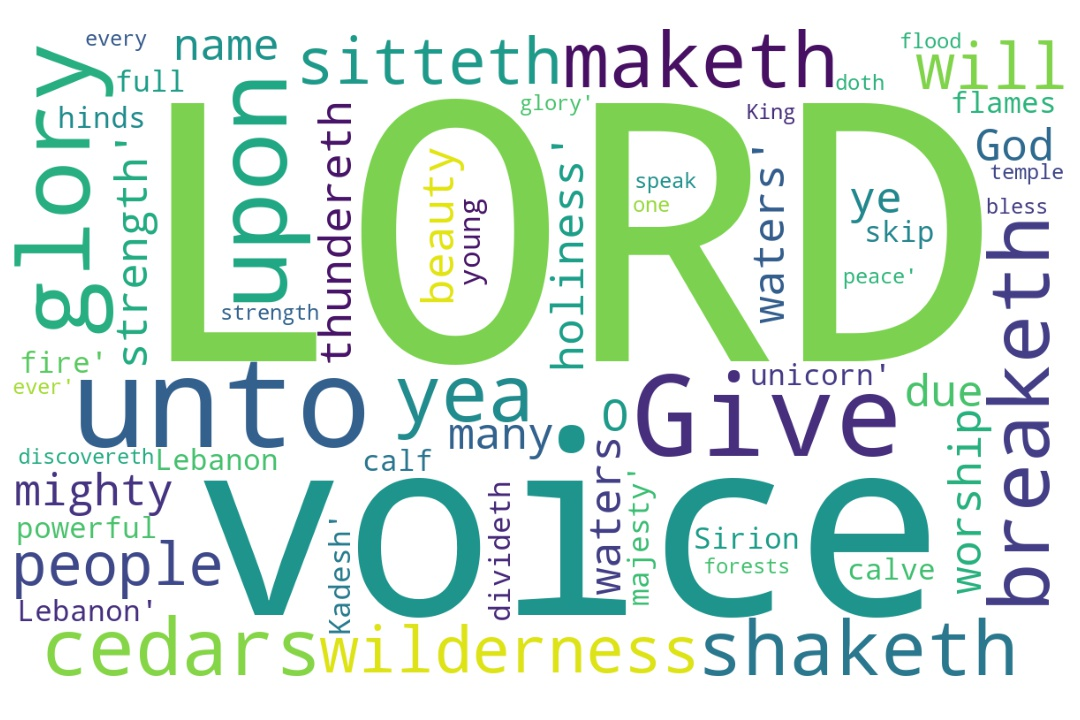
\includegraphics[width=\linewidth]{19OT-Psalms/Psalm29-WordCloud.jpg}
  \caption{Psalm 29 Word Cloud}
  \label{fig:Psalm 29 word Cloud}
\end{figure}


\marginpar{\scriptsize \centering \fcolorbox{bone}{lime}{\textbf{THE VOICE OF THE LORD}}\\ (Psalm 29:1-11) \begin{compactenum}[I.][8]
    \item \textbf{God's Place} \index[scripture]{Psalms!Psa 029:01}(Psa 29:1)
    \item \textbf{God's Presence Obvious} \index[scripture]{Psalms!Psa 029:03-09}(Psa 29:3-9)
    \item \textbf{God's Power Observed} \index[scripture]{Psalms!Psa 029:04}(Psa 29:4)
    \item \textbf{God's Peace Obtained} \index[scripture]{Psalms!Psa 029:11}(Psa 29:11)
    \item \textbf{God's People} \index[scripture]{Psalms!Psa 029:11}(Psa 29:11)
    \item \textbf{God's Preservation Ordained} \index[scripture]{Psalms!Psa 029:11}(Psa 29:11)
    \item \textbf{God's Providence}
\end{compactenum}}

\footnote{\textcolor[cmyk]{0.99998,1,0,0}{\hyperlink{TOC}{Return to end of Table of Contents.}}}\footnote{\href{https://www.audioverse.org/english/audiobibles/books/ENGKJV/O/Ps/1}{\textcolor[cmyk]{0.99998,1,0,0}{Psalms Audio}}}\textcolor[cmyk]{0.99998,1,0,0}{Give unto the LORD, O ye mighty, \fcolorbox{bone}{lime}{give unto the LORD} glory and strength.}
[2] \textcolor[cmyk]{0.99998,1,0,0}{Give unto the LORD the glory due unto his name; worship the LORD in the beauty of holiness.}
[3] \textcolor[cmyk]{0.99998,1,0,0}{The voice of the LORD \emph{is} upon the waters: the God of glory \fcolorbox{bone}{lime}{thundereth}: the LORD \emph{is} upon many waters.}
[4] \textcolor[cmyk]{0.99998,1,0,0}{The voice of the LORD \emph{is} \fcolorbox{bone}{lime}{powerful}; the voice of the LORD \emph{is} full of majesty.}
[5] \textcolor[cmyk]{0.99998,1,0,0}{The voice of the LORD breaketh the cedars; yea, the LORD breaketh the cedars of Lebanon.}
[6] \textcolor[cmyk]{0.99998,1,0,0}{He maketh them also to skip like a calf; Lebanon and Sirion like a young unicorn.}
[7] \textcolor[cmyk]{0.99998,1,0,0}{The voice of the LORD divideth the flames of fire.}
[8] \textcolor[cmyk]{0.99998,1,0,0}{The voice of the LORD shaketh the wilderness; the LORD shaketh the wilderness of Kadesh.}
[9] \textcolor[cmyk]{0.99998,1,0,0}{The voice of the LORD maketh the hinds to calve, and discovereth the forests: and in his temple doth every one speak of \emph{his} glory.}
[10] \textcolor[cmyk]{0.99998,1,0,0}{The LORD sitteth upon the flood; yea, the LORD sitteth King for ever.}
[11] \textcolor[cmyk]{0.99998,1,0,0}{The LORD will give strength unto his \fcolorbox{bone}{lime}{people}; the LORD will bless his people with \fcolorbox{bone}{lime}{peace}.}



\index[NWIV]{14!Psalms!Psa 29:1}\index[AWIP]{Give!Psalms!Psa 29:1}\index[AWIP]{unto!Psalms!Psa 29:1}\index[AWIP]{unto!Psalms!Psa 29:1 (2)}\index[AWIP]{the!Psalms!Psa 29:1}\index[AWIP]{the!Psalms!Psa 29:1 (2)}\index[AWIP]{LORD!Psalms!Psa 29:1}\index[AWIP]{LORD!Psalms!Psa 29:1 (2)}\index[AWIP]{O!Psalms!Psa 29:1}\index[AWIP]{ye!Psalms!Psa 29:1}\index[AWIP]{mighty!Psalms!Psa 29:1}\index[AWIP]{give!Psalms!Psa 29:1}\index[AWIP]{glory!Psalms!Psa 29:1}\index[AWIP]{and!Psalms!Psa 29:1}\index[AWIP]{strength!Psalms!Psa 29:1}

\index[NWIV]{18!Psalms!Psa 29:2}\index[AWIP]{Give!Psalms!Psa 29:2}\index[AWIP]{unto!Psalms!Psa 29:2}\index[AWIP]{unto!Psalms!Psa 29:2 (2)}\index[AWIP]{the!Psalms!Psa 29:2}\index[AWIP]{the!Psalms!Psa 29:2 (2)}\index[AWIP]{the!Psalms!Psa 29:2 (3)}\index[AWIP]{the!Psalms!Psa 29:2 (4)}\index[AWIP]{LORD!Psalms!Psa 29:2}\index[AWIP]{LORD!Psalms!Psa 29:2 (2)}\index[AWIP]{glory!Psalms!Psa 29:2}\index[AWIP]{due!Psalms!Psa 29:2}\index[AWIP]{his!Psalms!Psa 29:2}\index[AWIP]{name!Psalms!Psa 29:2}\index[AWIP]{worship!Psalms!Psa 29:2}\index[AWIP]{in!Psalms!Psa 29:2}\index[AWIP]{beauty!Psalms!Psa 29:2}\index[AWIP]{of!Psalms!Psa 29:2}\index[AWIP]{holiness!Psalms!Psa 29:2}

\index[NWIV]{20!Psalms!Psa 29:3}\index[AWIP]{The!Psalms!Psa 29:3}\index[AWIP]{voice!Psalms!Psa 29:3}\index[AWIP]{of!Psalms!Psa 29:3}\index[AWIP]{of!Psalms!Psa 29:3 (2)}\index[AWIP]{the!Psalms!Psa 29:3}\index[AWIP]{the!Psalms!Psa 29:3 (2)}\index[AWIP]{the!Psalms!Psa 29:3 (3)}\index[AWIP]{the!Psalms!Psa 29:3 (4)}\index[AWIP]{LORD!Psalms!Psa 29:3}\index[AWIP]{LORD!Psalms!Psa 29:3 (2)}\index[AWIP]{\emph{is}!Psalms!Psa 29:3}\index[AWIP]{\emph{is}!Psalms!Psa 29:3 (2)}\index[AWIP]{upon!Psalms!Psa 29:3}\index[AWIP]{upon!Psalms!Psa 29:3 (2)}\index[AWIP]{waters!Psalms!Psa 29:3}\index[AWIP]{waters!Psalms!Psa 29:3 (2)}\index[AWIP]{God!Psalms!Psa 29:3}\index[AWIP]{glory!Psalms!Psa 29:3}\index[AWIP]{thundereth!Psalms!Psa 29:3}\index[AWIP]{many!Psalms!Psa 29:3}\index[AWIP]{\emph{is}!Psalms!Psa 29:3}\index[AWIP]{\emph{is}!Psalms!Psa 29:3 (2)}

\index[NWIV]{16!Psalms!Psa 29:4}\index[AWIP]{The!Psalms!Psa 29:4}\index[AWIP]{voice!Psalms!Psa 29:4}\index[AWIP]{voice!Psalms!Psa 29:4 (2)}\index[AWIP]{of!Psalms!Psa 29:4}\index[AWIP]{of!Psalms!Psa 29:4 (2)}\index[AWIP]{of!Psalms!Psa 29:4 (3)}\index[AWIP]{the!Psalms!Psa 29:4}\index[AWIP]{the!Psalms!Psa 29:4 (2)}\index[AWIP]{the!Psalms!Psa 29:4 (3)}\index[AWIP]{LORD!Psalms!Psa 29:4}\index[AWIP]{LORD!Psalms!Psa 29:4 (2)}\index[AWIP]{\emph{is}!Psalms!Psa 29:4}\index[AWIP]{\emph{is}!Psalms!Psa 29:4 (2)}\index[AWIP]{powerful!Psalms!Psa 29:4}\index[AWIP]{full!Psalms!Psa 29:4}\index[AWIP]{majesty!Psalms!Psa 29:4}\index[AWIP]{\emph{is}!Psalms!Psa 29:4}\index[AWIP]{\emph{is}!Psalms!Psa 29:4 (2)}

\index[NWIV]{16!Psalms!Psa 29:5}\index[AWIP]{The!Psalms!Psa 29:5}\index[AWIP]{voice!Psalms!Psa 29:5}\index[AWIP]{of!Psalms!Psa 29:5}\index[AWIP]{of!Psalms!Psa 29:5 (2)}\index[AWIP]{the!Psalms!Psa 29:5}\index[AWIP]{the!Psalms!Psa 29:5 (2)}\index[AWIP]{the!Psalms!Psa 29:5 (3)}\index[AWIP]{the!Psalms!Psa 29:5 (4)}\index[AWIP]{LORD!Psalms!Psa 29:5}\index[AWIP]{LORD!Psalms!Psa 29:5 (2)}\index[AWIP]{breaketh!Psalms!Psa 29:5}\index[AWIP]{breaketh!Psalms!Psa 29:5 (2)}\index[AWIP]{cedars!Psalms!Psa 29:5}\index[AWIP]{cedars!Psalms!Psa 29:5 (2)}\index[AWIP]{yea!Psalms!Psa 29:5}\index[AWIP]{Lebanon!Psalms!Psa 29:5}

\index[NWIV]{16!Psalms!Psa 29:6}\index[AWIP]{He!Psalms!Psa 29:6}\index[AWIP]{maketh!Psalms!Psa 29:6}\index[AWIP]{them!Psalms!Psa 29:6}\index[AWIP]{also!Psalms!Psa 29:6}\index[AWIP]{to!Psalms!Psa 29:6}\index[AWIP]{skip!Psalms!Psa 29:6}\index[AWIP]{like!Psalms!Psa 29:6}\index[AWIP]{like!Psalms!Psa 29:6 (2)}\index[AWIP]{a!Psalms!Psa 29:6}\index[AWIP]{a!Psalms!Psa 29:6 (2)}\index[AWIP]{calf!Psalms!Psa 29:6}\index[AWIP]{Lebanon!Psalms!Psa 29:6}\index[AWIP]{and!Psalms!Psa 29:6}\index[AWIP]{Sirion!Psalms!Psa 29:6}\index[AWIP]{young!Psalms!Psa 29:6}\index[AWIP]{unicorn!Psalms!Psa 29:6}

\index[NWIV]{10!Psalms!Psa 29:7}\index[AWIP]{The!Psalms!Psa 29:7}\index[AWIP]{voice!Psalms!Psa 29:7}\index[AWIP]{of!Psalms!Psa 29:7}\index[AWIP]{of!Psalms!Psa 29:7 (2)}\index[AWIP]{the!Psalms!Psa 29:7}\index[AWIP]{the!Psalms!Psa 29:7 (2)}\index[AWIP]{LORD!Psalms!Psa 29:7}\index[AWIP]{divideth!Psalms!Psa 29:7}\index[AWIP]{flames!Psalms!Psa 29:7}\index[AWIP]{fire!Psalms!Psa 29:7}

\index[NWIV]{15!Psalms!Psa 29:8}\index[AWIP]{The!Psalms!Psa 29:8}\index[AWIP]{voice!Psalms!Psa 29:8}\index[AWIP]{of!Psalms!Psa 29:8}\index[AWIP]{of!Psalms!Psa 29:8 (2)}\index[AWIP]{the!Psalms!Psa 29:8}\index[AWIP]{the!Psalms!Psa 29:8 (2)}\index[AWIP]{the!Psalms!Psa 29:8 (3)}\index[AWIP]{the!Psalms!Psa 29:8 (4)}\index[AWIP]{LORD!Psalms!Psa 29:8}\index[AWIP]{LORD!Psalms!Psa 29:8 (2)}\index[AWIP]{shaketh!Psalms!Psa 29:8}\index[AWIP]{shaketh!Psalms!Psa 29:8 (2)}\index[AWIP]{wilderness!Psalms!Psa 29:8}\index[AWIP]{wilderness!Psalms!Psa 29:8 (2)}\index[AWIP]{Kadesh!Psalms!Psa 29:8}

\index[NWIV]{25!Psalms!Psa 29:9}\index[AWIP]{The!Psalms!Psa 29:9}\index[AWIP]{voice!Psalms!Psa 29:9}\index[AWIP]{of!Psalms!Psa 29:9}\index[AWIP]{of!Psalms!Psa 29:9 (2)}\index[AWIP]{the!Psalms!Psa 29:9}\index[AWIP]{the!Psalms!Psa 29:9 (2)}\index[AWIP]{the!Psalms!Psa 29:9 (3)}\index[AWIP]{LORD!Psalms!Psa 29:9}\index[AWIP]{maketh!Psalms!Psa 29:9}\index[AWIP]{hinds!Psalms!Psa 29:9}\index[AWIP]{to!Psalms!Psa 29:9}\index[AWIP]{calve!Psalms!Psa 29:9}\index[AWIP]{and!Psalms!Psa 29:9}\index[AWIP]{and!Psalms!Psa 29:9 (2)}\index[AWIP]{discovereth!Psalms!Psa 29:9}\index[AWIP]{forests!Psalms!Psa 29:9}\index[AWIP]{in!Psalms!Psa 29:9}\index[AWIP]{his!Psalms!Psa 29:9}\index[AWIP]{temple!Psalms!Psa 29:9}\index[AWIP]{doth!Psalms!Psa 29:9}\index[AWIP]{every!Psalms!Psa 29:9}\index[AWIP]{one!Psalms!Psa 29:9}\index[AWIP]{speak!Psalms!Psa 29:9}\index[AWIP]{\emph{his}!Psalms!Psa 29:9}\index[AWIP]{glory!Psalms!Psa 29:9}\index[AWIP]{\emph{his}!Psalms!Psa 29:9}

\index[NWIV]{13!Psalms!Psa 29:10}\index[AWIP]{The!Psalms!Psa 29:10}\index[AWIP]{LORD!Psalms!Psa 29:10}\index[AWIP]{LORD!Psalms!Psa 29:10 (2)}\index[AWIP]{sitteth!Psalms!Psa 29:10}\index[AWIP]{sitteth!Psalms!Psa 29:10 (2)}\index[AWIP]{upon!Psalms!Psa 29:10}\index[AWIP]{the!Psalms!Psa 29:10}\index[AWIP]{the!Psalms!Psa 29:10 (2)}\index[AWIP]{flood!Psalms!Psa 29:10}\index[AWIP]{yea!Psalms!Psa 29:10}\index[AWIP]{King!Psalms!Psa 29:10}\index[AWIP]{for!Psalms!Psa 29:10}\index[AWIP]{ever!Psalms!Psa 29:10}

\index[NWIV]{16!Psalms!Psa 29:11}\index[AWIP]{The!Psalms!Psa 29:11}\index[AWIP]{LORD!Psalms!Psa 29:11}\index[AWIP]{LORD!Psalms!Psa 29:11 (2)}\index[AWIP]{will!Psalms!Psa 29:11}\index[AWIP]{will!Psalms!Psa 29:11 (2)}\index[AWIP]{give!Psalms!Psa 29:11}\index[AWIP]{strength!Psalms!Psa 29:11}\index[AWIP]{unto!Psalms!Psa 29:11}\index[AWIP]{his!Psalms!Psa 29:11}\index[AWIP]{his!Psalms!Psa 29:11 (2)}\index[AWIP]{people!Psalms!Psa 29:11}\index[AWIP]{people!Psalms!Psa 29:11 (2)}\index[AWIP]{the!Psalms!Psa 29:11}\index[AWIP]{bless!Psalms!Psa 29:11}\index[AWIP]{with!Psalms!Psa 29:11}\index[AWIP]{peace!Psalms!Psa 29:11}


\section{Psalm 29 Outlines}

\subsection{My Outlines}

\subsubsection{The Voice of the Lord}

\index[speaker]{Keith Anthony!Psalm 029 (The Voice of the Lord)}
\index[series]{Psalms (Keith Anthony)!Psalm 029 (The Voice of the Lord)}
\index[date]{unknown!Psalm 029 (The Voice of the Lord) (Keith Anthony)}
\begin{compactenum}[I.]
    \item \textbf{God's Place} \index[scripture]{Psalms!Psa 029:01}(Psa 29:1)
    \item \textbf{God's Presence Obvious} \index[scripture]{Psalms!Psa 029:03-09}(Psa 29:3-9)
    \item \textbf{God's Power Observed} \index[scripture]{Psalms!Psa 029:04}(Psa 29:4)
    \item \textbf{God's Peace Obtained} \index[scripture]{Psalms!Psa 029:11}(Psa 29:11)
    \item \textbf{God's People} \index[scripture]{Psalms!Psa 029:11}(Psa 29:11)
    \item \textbf{God's Preservation Ordained} \index[scripture]{Psalms!Psa 029:11}(Psa 29:11)
    \item \textbf{God's Providence}
\end{compactenum}

\subsection{Outlines from Others}
\section{Psalm 29 Comments}

\subsection{Numeric Nuggets}
\textbf{13:} There are 13 words in Psalm 29:10. There are 13 unique words in verse 2.

\subsection{Introduction}
Compare with Psalm 1. Here David walks in integrity (Psalm 26:1), stands in an even place (Psalm 26:12), and does not sit with vain persons or evil doer (Psalm 26:4, 5).

\subsection{Psalm 29 Repeated Phrases}


%%%%%%%%%%
%%%%%%%%%%
\normalsize
 
\begin{center}
\begin{longtable}{|c|c|}
\caption[Psalm 29 Repeated Phrases]{Psalm2 9 Repeated Phrases}\label{table:Repeated Phrases Psalm 29} \\
\hline \multicolumn{1}{|c|}{\textbf{Phrase}} & \multicolumn{1}{c|}{\textbf{Frequency}} \\ \hline 
\endfirsthead
 
\multicolumn{2}{c}
{{\bfseries \tablename\ \thetable{} -- continued from previous page}} \\  
\hline \multicolumn{1}{|c|}{\textbf{Phrase}} & \multicolumn{1}{c|}{\textbf{Frequency}} \\ \hline 
\endhead
 
\hline \multicolumn{2}{c}{{ }} \\ \hline
\endfoot 
the LORD & 16\\ \hline 
voice of & 7\\ \hline 
voice of the & 7\\ \hline 
voice of the LORD & 7\\ \hline 
of the & 7\\ \hline 
of the LORD & 7\\ \hline 
The voice & 6\\ \hline 
The voice of & 6\\ \hline 
The voice of the & 6\\ \hline 
The voice of the LORD & 6\\ \hline 
the LORD \emph{is} & 4\\ \hline 
LORD \emph{is} & 4\\ \hline 
unto the & 3\\ \hline 
unto the LORD & 3\\ \hline 
voice of the LORD \emph{is} & 3\\ \hline 
of the LORD \emph{is} & 3\\ \hline 
\end{longtable}
\end{center}



%%%%%%%%%%
%%%%%%%%%%



\section{Psalm 29 Statistics}

%%%%%%%%%%%%%%%%%%%%%%%%%%%
%%%%% Word Statistics
%%%%%%%%%%%%%%%%%%%%%%%%%%


\normalsize



\subsection{Chapter Word Statistics}


%%%%%%%%%%
%%%%%%%%%%
 
\begin{center}
\begin{longtable}{l|c|c|c|c}
\caption[Stats for Psalm 29]{Stats for Psalm 29} \label{table:Stats for Psalm 29} \\ 
\hline \multicolumn{1}{|c|}{\textbf{Verse(s)}} & \multicolumn{1}{|c|}{\textbf{Count}} & \multicolumn{1}{|c|}{\textbf{Unique}} & \multicolumn{1}{|c|}{\textbf{Italics}} & \multicolumn{1}{|c|}{\textbf{Uniq Italic}}  \\ \hline 
\endfirsthead
 
\multicolumn{5}{c}
{{\bfseries \tablename\ \thetable{} -- continued from previous page}} \\  
\hline \multicolumn{1}{|c|}{\textbf{Verse(s)}} & \multicolumn{1}{|c|}{\textbf{Count}} & \multicolumn{1}{|c|}{\textbf{Unique}} & \multicolumn{1}{|c|}{\textbf{Italics}} & \multicolumn{1}{|c|}{\textbf{Uniq Italic}}  \\ \hline 
\endhead
 
\hline \multicolumn{5}{|r|}{{Continued if needed}} \\ \hline
\endfoot 
1 & 14 & 11 & 0 & 0\\ \hline
2 & 18 & 13 & 0 & 0\\ \hline
3 & 20 & 12 & 2 & 1\\ \hline
4 & 16 & 9 & 2 & 1\\ \hline
5 & 16 & 9 & 0 & 0\\ \hline
6 & 16 & 14 & 0 & 0\\ \hline
7 & 10 & 8 & 0 & 0\\ \hline
8 & 15 & 8 & 0 & 0\\ \hline
9 & 25 & 21 & 1 & 1\\ \hline
10 & 13 & 10 & 0 & 0\\ \hline
11 & 16 & 12 & 0 & 0\\ \hline
\hline \hline
Total & 179 & 72 & 5 & 2



\end{longtable}
\end{center}

%%%%%%%%%%
%%%%%%%%%%
 
\subsection{Words by Frequency}

\begin{center}
\begin{longtable}{l|r}
\caption[Word Frequencies in Psalm 29]{Word Frequencies in Psalm 29} \label{table:WordsIn-Psalm-29} \\ 
\hline \multicolumn{1}{|c|}{\textbf{Word}} & \multicolumn{1}{c|}{\textbf{Frequency}} \\ \hline 
\endfirsthead
 
\multicolumn{2}{c}
{{\bfseries \tablename\ \thetable{} -- continued from previous page}} \\ 
\hline \multicolumn{1}{|c|}{\textbf{Word}} & \multicolumn{1}{c|}{\textbf{Frequency}} \\ \hline 
\endhead
 
\hline \multicolumn{2}{|r|}{{Continued if needed}} \\ \hline
\endfoot
 
\hline \hline
\endlastfoot
the & 29 \\ \hline
LORD & 18 \\ \hline
of & 14 \\ \hline
The & 8 \\ \hline
voice & 7 \\ \hline
unto & 5 \\ \hline
glory & 4 \\ \hline
and & 4 \\ \hline
his & 4 \\ \hline
\emph{is} & 4 \\ \hline
upon & 3 \\ \hline
Give & 2 \\ \hline
give & 2 \\ \hline
strength & 2 \\ \hline
in & 2 \\ \hline
waters & 2 \\ \hline
breaketh & 2 \\ \hline
cedars & 2 \\ \hline
yea & 2 \\ \hline
Lebanon & 2 \\ \hline
maketh & 2 \\ \hline
to & 2 \\ \hline
like & 2 \\ \hline
a & 2 \\ \hline
shaketh & 2 \\ \hline
wilderness & 2 \\ \hline
sitteth & 2 \\ \hline
will & 2 \\ \hline
people & 2 \\ \hline
O & 1 \\ \hline
ye & 1 \\ \hline
mighty & 1 \\ \hline
due & 1 \\ \hline
name & 1 \\ \hline
worship & 1 \\ \hline
beauty & 1 \\ \hline
holiness & 1 \\ \hline
God & 1 \\ \hline
thundereth & 1 \\ \hline
many & 1 \\ \hline
powerful & 1 \\ \hline
full & 1 \\ \hline
majesty & 1 \\ \hline
He & 1 \\ \hline
them & 1 \\ \hline
also & 1 \\ \hline
skip & 1 \\ \hline
calf & 1 \\ \hline
Sirion & 1 \\ \hline
young & 1 \\ \hline
unicorn & 1 \\ \hline
divideth & 1 \\ \hline
flames & 1 \\ \hline
fire & 1 \\ \hline
Kadesh & 1 \\ \hline
hinds & 1 \\ \hline
calve & 1 \\ \hline
discovereth & 1 \\ \hline
forests & 1 \\ \hline
temple & 1 \\ \hline
doth & 1 \\ \hline
every & 1 \\ \hline
one & 1 \\ \hline
speak & 1 \\ \hline
\emph{his} & 1 \\ \hline
flood & 1 \\ \hline
King & 1 \\ \hline
for & 1 \\ \hline
ever & 1 \\ \hline
bless & 1 \\ \hline
with & 1 \\ \hline
peace & 1 \\ \hline
\end{longtable}
\end{center}



\normalsize



\subsection{Words Alphabetically}

\begin{center}
\begin{longtable}{l|r}
\caption[Word Alphabetically in Psalm 29]{Word Alphabetically in Psalm 29} \label{table:WordsIn-Psalm-29} \\ 
\hline \multicolumn{1}{|c|}{\textbf{Word}} & \multicolumn{1}{c|}{\textbf{Frequency}} \\ \hline 
\endfirsthead
 
\multicolumn{2}{c}
{{\bfseries \tablename\ \thetable{} -- continued from previous page}} \\ 
\hline \multicolumn{1}{|c|}{\textbf{Word}} & \multicolumn{1}{c|}{\textbf{Frequency}} \\ \hline 
\endhead
 
\hline \multicolumn{2}{|r|}{{Continued if needed}} \\ \hline
\endfoot
 
\hline \hline
\endlastfoot
Give & 2 \\ \hline
God & 1 \\ \hline
He & 1 \\ \hline
Kadesh & 1 \\ \hline
King & 1 \\ \hline
LORD & 18 \\ \hline
Lebanon & 2 \\ \hline
O & 1 \\ \hline
Sirion & 1 \\ \hline
The & 8 \\ \hline
\emph{his} & 1 \\ \hline
\emph{is} & 4 \\ \hline
a & 2 \\ \hline
also & 1 \\ \hline
and & 4 \\ \hline
beauty & 1 \\ \hline
bless & 1 \\ \hline
breaketh & 2 \\ \hline
calf & 1 \\ \hline
calve & 1 \\ \hline
cedars & 2 \\ \hline
discovereth & 1 \\ \hline
divideth & 1 \\ \hline
doth & 1 \\ \hline
due & 1 \\ \hline
ever & 1 \\ \hline
every & 1 \\ \hline
fire & 1 \\ \hline
flames & 1 \\ \hline
flood & 1 \\ \hline
for & 1 \\ \hline
forests & 1 \\ \hline
full & 1 \\ \hline
give & 2 \\ \hline
glory & 4 \\ \hline
hinds & 1 \\ \hline
his & 4 \\ \hline
holiness & 1 \\ \hline
in & 2 \\ \hline
like & 2 \\ \hline
majesty & 1 \\ \hline
maketh & 2 \\ \hline
many & 1 \\ \hline
mighty & 1 \\ \hline
name & 1 \\ \hline
of & 14 \\ \hline
one & 1 \\ \hline
peace & 1 \\ \hline
people & 2 \\ \hline
powerful & 1 \\ \hline
shaketh & 2 \\ \hline
sitteth & 2 \\ \hline
skip & 1 \\ \hline
speak & 1 \\ \hline
strength & 2 \\ \hline
temple & 1 \\ \hline
the & 29 \\ \hline
them & 1 \\ \hline
thundereth & 1 \\ \hline
to & 2 \\ \hline
unicorn & 1 \\ \hline
unto & 5 \\ \hline
upon & 3 \\ \hline
voice & 7 \\ \hline
waters & 2 \\ \hline
wilderness & 2 \\ \hline
will & 2 \\ \hline
with & 1 \\ \hline
worship & 1 \\ \hline
ye & 1 \\ \hline
yea & 2 \\ \hline
young & 1 \\ \hline
\end{longtable}
\end{center}



\normalsize



\subsection{Word Lengths in Chapter}
\normalsize
\begin{longtable}{l|p{3.75in}}
\caption[Words by Length in Psalm 29]{Words by Length in Psalm 29} \label{table:WordsIn-Psalm-29} \\ 
\hline \multicolumn{1}{|c|}{\textbf{Length}} & \multicolumn{1}{c|}{\textbf{Words}} \\ \hline 
\endfirsthead
 
\multicolumn{2}{c}
{{\bfseries \tablename\ \thetable{} -- continued from previous page}} \\ 
\hline \multicolumn{1}{|c|}{\textbf{Length}} & \multicolumn{1}{c|}{\textbf{Words}} \\ \hline 
\endhead
 
\hline \multicolumn{2}{|r|}{{Continued if needed}} \\ \hline
\endfoot
 
\hline \hline
\endlastfoot
1 & O, a \\ \hline
2 & ye, in, of, \emph{is}, He, to \\ \hline
3 & the, and, due, his, The, God, yea, one, \emph{his}, for \\ \hline
4 & Give, unto, LORD, give, name, upon, many, full, them, also, skip, like, calf, fire, doth, King, ever, will, with \\ \hline
5 & glory, voice, young, hinds, calve, every, speak, flood, bless, peace \\ \hline
6 & mighty, beauty, waters, cedars, maketh, Sirion, flames, Kadesh, temple, people \\ \hline
7 & worship, majesty, Lebanon, unicorn, shaketh, forests, sitteth \\ \hline
8 & strength, holiness, powerful, breaketh, divideth \\ \hline
10 & thundereth, wilderness \\ \hline
11 & discovereth \\ \hline
\end{longtable}






%%%%%%%%%%
%%%%%%%%%%
 



%%%%%%%%%%
%%%%%%%%%%
\subsection{Verses with 13 Words in Chapter}
\normalsize
\begin{longtable}{l|p{3.75in}}
\caption[Verses with 13 Words  in Psalm 29]{Verses with 13 Words  in Psalm 29} \label{table:Verses with 13 Words in-Psalm-29} \\ 
\hline \multicolumn{1}{|c|}{\textbf{Reference}} & \multicolumn{1}{c|}{\textbf{Verse}} \\ \hline 
\endfirsthead
 
\multicolumn{2}{c}
{{\bfseries \tablename\ \thetable{} -- continued from previous page}} \\ 
\hline \multicolumn{1}{|c|}{\textbf{Reference}} & \multicolumn{1}{c|}{\textbf{Verse}} \\ \hline 
\endhead
 
\hline \multicolumn{2}{|r|}{{Continued if needed}} \\ \hline
\endfoot
 
\hline \hline
\endlastfoot
Psalms 029:10 & The LORD sitteth upon the flood; yea, the LORD sitteth King for ever. \\ \hline
\end{longtable}






%%%%%%%%%%
%%%%%%%%%%
 



%%%%%%%%%%
%%%%%%%%%%
\subsection{Verses with 18 Words in Chapter}
\normalsize
\begin{longtable}{l|p{3.75in}}
\caption[Verses with 18 Words  in Psalm 29]{Verses with 18 Words  in Psalm 29} \label{table:Verses with 18 Words in-Psalm-29} \\ 
\hline \multicolumn{1}{|c|}{\textbf{Reference}} & \multicolumn{1}{c|}{\textbf{Verse}} \\ \hline 
\endfirsthead
 
\multicolumn{2}{c}
{{\bfseries \tablename\ \thetable{} -- continued from previous page}} \\ 
\hline \multicolumn{1}{|c|}{\textbf{Reference}} & \multicolumn{1}{c|}{\textbf{Verse}} \\ \hline 
\endhead
 
\hline \multicolumn{2}{|r|}{{Continued if needed}} \\ \hline
\endfoot
 
\hline \hline
\endlastfoot
Psalms 029:2 & Give unto the LORD the glory due unto his name; worship the LORD in the beauty of holiness. \\ \hline
\end{longtable}






%%%%%%%%%%
%%%%%%%%%%
%%%%%%%%%%

\chapter{Proverbs Introduction}

\section{Some Statistics about 13 in Proverbs}

\begin{center}
\begin{longtable}{p{0.4in}|p{1.5in}|p{2.6in}}

\caption[Words Thirteen Times in the Proverbs Chapters]{Words Thirteen Times in the Proverbs Chapters} \label{table:Stats-PRO-13-TIC} \\ 
\hline \multicolumn{1}{|c|}{\textbf{Chapter}} & 
\multicolumn{1}{|c|}{\textbf{Word}} & 
\multicolumn{1}{|c|}{\textbf{Comment}}   \\ \hline 
\endfirsthead
 
\multicolumn{3}{c}
{{\bfseries \tablename\ \thetable{} -- continued from previous page}} \\  
\hline \multicolumn{1}{|c|}{\textbf{Chapter}} & 
\multicolumn{1}{|c|}{\textbf{Word}} & 
\multicolumn{1}{|c|}{\textbf{Comment}}  \\ \hline 
\endhead
 
\hline \multicolumn{3}{|r|}{{Continued as needed}} \\ \hline
\endfoot 
1--3 & \textbf{\textcolor[rgb]{0.00,1.00,0.00}{NONE}}  &\\ \hline
4 & not & \\ \hline
5 & \textbf{\textcolor[rgb]{0.00,1.00,0.00}{NONE}} & \\ \hline
6 & his & \\ \hline
7 & \textbf{\textcolor[rgb]{0.00,1.00,0.00}{NONE}} & \\ \hline
8 & me & \\ \hline
9--10 & \textbf{\textcolor[rgb]{0.00,1.00,0.00}{NONE}} & \\ \hline
11 & \emph{is}, a, his & \\ \hline
12 & a & \\ \hline
13 & shall & \\ \hline
14 & \textbf{\textcolor[rgb]{0.00,1.00,0.00}{NONE}} & \\ \hline
15 & that & \\ \hline
16--17 & \textbf{\textcolor[rgb]{0.00,1.00,0.00}{NONE}} & \\ \hline
18 & his & \\ \hline
19--20 & \textbf{\textcolor[rgb]{0.00,1.00,0.00}{NONE}} & \\ \hline
21 & his & \\ \hline
22 & of & \\ \hline
23 & of & \\ \hline
24--25 & \textbf{\textcolor[rgb]{0.00,1.00,0.00}{NONE}} & \\ \hline
26 & in & \\ \hline
27 & \emph{is} &\\ \hline
28 & \emph{is} & \\ \hline
29 & but, his \\ \hline
30--31 & \textbf{\textcolor[rgb]{0.00,1.00,0.00}{NONE}} & \\ \hline
\hline \hline
%Total & 594 & 224 & 22 & 12



\end{longtable}
\end{center}


\begin{center}
\begin{longtable}{c|c|p{3.5in}}
\caption[Verses with 13 Words in Proverbs]{Verses with 13 Words in Proverbs} \label{table:Stats-PRO-13-VWTW} \\ 
\hline \multicolumn{1}{|c|}{\textbf{Chapter}} & 
\multicolumn{1}{|c|}{\textbf{Verse}} & 
\multicolumn{1}{|l|}{\textbf{Comment}}   \\ \hline 
\endfirsthead
 
\multicolumn{3}{c}
{{\bfseries \tablename\ \thetable{} -- continued from previous page}} \\  
\hline \multicolumn{1}{|c|}{\textbf{Chapter}} & 
\multicolumn{1}{|c|}{\textbf{Verse}} & 
\multicolumn{1}{|l|}{\textbf{Comment}}  \\ \hline 
\endhead
 
\hline \multicolumn{3}{|r|}{{Continued as needed}} \\ \hline
\endfoot 
1 & 1:4 & To give subtilty to the simple, to the young man knowledge and discretion.  \\ 
1 & 1:13 & We shall find all precious substance, we shall fill our houses with spoil:   \\ 
1 & 1:17 & Surely in vain the net is spread in the sight of any bird.  \\ \hline
2 & 2:3 &  Yea, if thou criest after knowledge, and liftest up thy voice for understanding; \\ 
2 & 2:6 & For the LORD giveth wisdom: out of his mouth cometh knowledge and understanding. \\ 
2 & 2:8 & He keepeth the paths of judgment, and preserveth the way of his saints. \\ 
2 & 2:9 & Then shalt thou understand righteousness, and judgment, and equity; yea, every good path. \\ 
2 & 2:10 & When wisdom entereth into thine heart, and knowledge is pleasant unto thy
soul; \\ 
2 & 2:13 & Who leave the paths of uprightness, to walk in the ways of darkness; \\ 
2 & 2:14 & Who rejoice to do evil, and delight in the frowardness of the wicked; \\ \hline
3 & 3:1 & My son, forget not my law; but let thine heart keep my commandments: \\ 
3 & 3:13 & Happy is the man that findeth wisdom, and the man that getteth understanding. \\ 
3 & 3:22 &  So shall they be life unto thy soul, and grace to thy neck. \\ 
3 & 3:35 & The wise shall inherit glory: but shame shall be the promotion of fools. \\ \hline
4 & 4:1 & Hear,  ye children, the instruction of a father, and attend to know understanding. \\ 
4 & 4:17 & For they eat the bread of wickedness, and drink the wine of violence. \\ 
4 & 4:26 &  Ponder the path of thy feet, and let all thy ways be established. \\  \hline
5 & 5:1  & My son, attend unto my wisdom, and bow thine ear to my understanding: \\ 
5 & 5:9  & Lest thou give thine honour unto others, and thy years unto the cruel: \\ 
5 & 5:16  & Let thy fountains be dispersed abroad, and rivers of waters in the streets. \\ 
5 & 5:18  & Let thy fountain be blessed: and rejoice with the wife of thy youth.   \\  \hline
6 & 6:8  & Provideth her meat in the summer, and gathereth her food in the harvest.  \\ 
6 & 6:15  &  Therefore shall his calamity come suddenly; suddenly shall he be broken without remedy.\\ 
6 & 6:19  & A false witness that speaketh lies, and he that soweth discord among brethren.  \\  \hline
7 & 7:3  & Bind them upon thy fingers, write them upon the table of thine heart.  \\ 
7 & 7:14  &   I have peace offerings with me; this day have I payed my vows. \\ 
7 & 7:19  & For the goodman is not at home, he is gone a long journey: \\ \hline
8 & 8:16  &  Length of days is in her right hand; and in her left hand riches and honour. \\ 
8 & 8:35  & The wise shall inherit glory: but shame shall be the promotion of fools. \\  \hline
9 & \textbf{\textcolor[rgb]{0.00,1.00,0.00}{NONE}}  &\\ \hline
10 & 10:8  & The wise in heart will receive commandments: but a prating fool shall fall. \\ \hline
11 & 11:4 & Riches profit not in the day of wrath: but righteousness delivereth from death.   \\ \hline
12 & \textbf{\textcolor[rgb]{0.00,1.00,0.00}{NONE}}  &\\ \hline
13 & 13:1 &   A   wise son heareth his father’s instruction: but a scorner heareth not rebuke. \\ 
13 & 13:16 &  Every prudent man dealeth with knowledge: but a fool layeth open his folly. \\ \hline
14 & 14:5 &  A faithful witness will not lie: but a false witness will utter lies. \\ 
14 & 14:9 & Fools make a mock at sin: but among the righteous there is favour.   \\  \hline
15 & 15:5 & A fool despiseth his father’s instruction: but he that regardeth reproof is prudent.  \\  \hline
16 & 16:26 & He that laboureth laboureth for himself; for his mouth craveth it of him.  \\  \hline
17 & 17:7 &  Excellent speech becometh not a fool: much less do lying lips a prince. \\  
17 & 17:17 &  A friend loveth at all times, and a brother is born for adversity. \\   \hline
18 & 18:1 & Through desire a man, having separated himself, seeketh and intermeddleth
with all wisdom.  \\  
18 & 18:12 & Before destruction the heart of man is haughty, and before honour is humility.  \\  
18 & 18:16 & A man’s gift maketh room for him, and bringeth him before great men.  \\  \hline
19 & 19:15 & Slothfulness casteth into a deep sleep; and an idle soul shall suffer hunger. \\ 
19 & 19:28 & An ungodly witness scorneth judgment: and the mouth of the wicked devoureth iniquity.  \\  \hline
20 & 20:7 & The just man walketh in his integrity: his
children are blessed after him.  \\  
20 & 20:28 & Mercy and truth preserve the king: and his throne is upholden by mercy.  \\  \hline
21 & 21:3 & To do justice and judgment is more acceptable to the LORD than sacrifice.  \\  
21 & 21:25 &  The desire of the slothful killeth him; for his hands refuse to labour.   \\   \hline
22 & \textbf{\textcolor[rgb]{0.00,1.00,0.00}{NONE}}  &\\ \hline
23 & 23:12 & Apply thine heart unto instruction, and thine ears to the words of knowledge.  \\ 
23 & 23:15 & My son, if thine heart be wise, my heart shall rejoice, even mine.\\
23 & 23:23 & Buy the truth, and sell it not; also wisdom, and instruction, and understanding. \\ 
23 & 23:26 & My son, give me thine heart, and let thine eyes observe my ways.\\ 
23 & 23:32 & At the last it biteth like a serpent, and stingeth like an adder. \\ 
23 & 23:33 & Thine eyes shall behold strange women, and thine heart shall utter perverse things. \\ \hline
24 & 24:1 & Be  not thou envious against evil men, neither desire to be with them. \\ \hline
25 & 25:11 & A word fitly spoken is like apples of gold in pictures of silver. \\ \hline
26 & 26:24 & He that hateth dissembleth with his lips, and layeth up deceit within him;\\ \hline
27 & \textbf{\textcolor[rgb]{0.00,1.00,0.00}{NONE}}  &\\ \hline
29 & 29:22 & An angry man stirreth up strife, and a furious man aboundeth in transgression.\\ 
29 & 29:26 & Many seek the ruler’s favour; but every man’s judgment cometh from the LORD\\ \hline
30 & 30:29 & There be three things which go well, yea, four are comely in going:\\ 
30 & 30:30 & A lion which is strongest among beasts, and turneth not away for any;\\ \hline
31 & 31:7 & Let him drink, and forget his poverty, and remember his misery no more.\\ 
31 & 31:24 & She maketh fine linen, and selleth it; and delivereth girdles unto the merchant.\\ 

\hline \hline



\end{longtable}
\end{center}


\begin{center}
\begin{longtable}{l|r}
\caption[13-Letter Words in Proverbs Chapters]{13-Letter Words in Proverbs Chapters} \label{table:PROVERBS-13LWFIS} \\ 
\hline \multicolumn{1}{|c|}{\textbf{Chapter}} & \multicolumn{1}{c|}{\textbf{Words}} \\ \hline 
\endfirsthead
 
\multicolumn{2}{c}
{{\bfseries \tablename\ \thetable{} -- continued from previous page}} \\ 
\hline \multicolumn{1}{|c|}{\textbf{Chapter}} & \multicolumn{1}{c|}{\textbf{Words}} \\ \hline 
\endhead
 
\hline \multicolumn{2}{|r|}{{Continued if needed}} \\ \hline
\endfoot
 
\hline \hline
\endlastfoot
%1 & uncircumcised \\ \hline
1 & understanding \\ \hline
2 & righteousness transgressors understanding \\ \hline
3 & understanding \\ \hline
4 & understanding \\ \hline
5 & understanding \\ \hline
6 & understanding \\ \hline
7 & understanding \\ \hline
8 & righteousness understandeth understanding \\ \hline
9 & understanding \\ \hline
10 & righteousness understanding \\ \hline
11 & righteousness transgressors understanding \\ \hline
12 & righteousness transgression understanding \\ \hline
13 & Righteousness transgressors understanding \\ \hline
14 & Righteousness understandeth understanding \\ \hline
15 & righteousness understanding \\ \hline
16 & Understanding righteousness transgresseth understanding \\ \hline
17 & transgression understanding whithersoever \\ \hline
18 & intermeddleth understanding \\ \hline
19 & transgression understanding \\ \hline
20 & understanding \\ \hline
21 & plenteousness righteousness understanding whithersoever \\ \hline
22 & \textbf{\textcolor[rgb]{0.00,1.00,0.00}{NONE}}  \\ \hline
23 & transgressors understanding \\ \hline
24 & understanding \\ \hline
25 & righteousness \\ \hline
26 & righteousness \\ \hline
27 & \textbf{\textcolor[rgb]{0.00,1.00,0.00}{NONE}}  \\ \hline
28 & transgression understanding \\ \hline
29 & transgression \\ \hline
30 & understanding \\ \hline
31 & strengtheneth \\ \hline



\end{longtable}
\end{center}

\section{Interesting}
It is interesting that the word ``the'' is used exactly 1000 time in Proverbs. In the book there are number of words and phrases found 13 times. Given that Proverbs is a ``wisdom'' book, we'd expect that this list would be insightful into wisdom concerning rebellion (consider Table ~\ref{table:13timesinproverbs}).

\subsection{Found 13 times in Proverbs}

\begin{center}
\begin{longtable}{l|p{3.75in}}
\caption[Found 13 times in Proverbs]{Found 13 times in Proverbs} \label{table:13timesinproverbs} \\ 
\hline \multicolumn{1}{|c|}{\textbf{Word or Phrase}} & \multicolumn{1}{c|}{\textbf{Location}} \\ \hline 
\endfirsthead
 
\multicolumn{2}{c}
{{\bfseries \tablename\ \thetable{} -- continued from previous page}} \\ 
\hline \multicolumn{1}{|c|}{\textbf{Word or Phrase}} & \multicolumn{1}{c|}{\textbf{Location}} \\ \hline 
\endhead
 
\hline \multicolumn{2}{|r|}{{Continued}} \\ \hline
\endfoot
 
\hline \hline
\endlastfoot
``if''\footnote{Also found 5 times in italics} & \\ \hline
``cause'' & Pro 1:11, 3:30, 4:16, 8:21, 18:17, 22:23, 23:11, 23:29, 24:28, 25:9, 29:7, 31:8, and 31:9 \\ \hline
``Let''\footnote{Also found 1 time in italics} & Pro 1:12, 3:3, 4:4, 4:21, 4:25, 5:16, 5:17, 5:18, 7:25, 17:12, 23:17, 27:2, and  31:7\\ \hline

``find'' & Pro 1:13, 1:28, 2:5, 3:4, 4:22, 8:9, 8:12, 8:17, 16:20, 19:8, 20:6, 28:23, and 31:10 \\ \hline

``among''\footnote{Proverb 30:14 has the word in italics.} & Pro 1:14, 6:19, 7:7 (2x),  14:9, 15:31, 17:2, 23:20 (2x), 23:28, 27:22, 30:14, 30:30, and 31:23\\ \hline

``one''\footnote{Proverb 3:18 and 22:26 have the word in italics.} & Pro 1:14, Pro 1:19, Pro 6:11, Pro 6:28, Pro 8:30, 15:12, Pro 16:5, Pro 17:14, Pro 19:25, Pro 20:6, Pro 21:5, Pro 24:34, and Pro 26:17  \\ \hline

``in the way''\footnote{Proverb 10:17 has the phrase partially in italics.} & Pro 1:15, Pro 2:20, Pro 4:11, Pro 4:14, Pro 8:20, Pro 9:6, Pro 13:6, Pro 16:31, Pro 22:5, Pro 22:6, Pro 23:19, Pro 26:13, and Pro 29:27
  \\ \hline
  
``\emph{which}''\footnote{There are 11 instances of the word  not in italics in Proverbs} & Pro 1:19, Pro 2:16, Pro 7:5, Pro 9:5, Pro 14:33, Pro 20:25, Pro 23:8, Pro 24:13, Pro 27:16 Pro 30:18 (once), Pro 30:21, Pro 30:24, and Pro 30:30 \\ \hline

``thereof''\footnote{The word also occurs italics once in Pro 12:28 and 28:22.} & Pro 1:19, Pro 3:14, Pro 14:12, Pro 16:25, Pro 16:33, Pro 18:21, Pro 20:21, Pro 21:22, Pro 24:31, Pro 25:8, Pro 27:18, and Pro 28:2 \\ \hline

``city'' & Pro  1:21, 8:3, 9:3, 9:14, 10:15, 11:10, 11:11, 16:32, 18:11, 18:19, 21:22,  25:28, and 29:8 \\ \hline


``reproof'' & Pro 1:23, 1:25, 1:30, 5:12, 10:17, 12:1, 13:18, 15:5, 15:10, 15:31, 15:32,  17:10, and 29:15 \\ \hline

``For the'' &  Pro  1:32, Pro 2:6, Pro 2:21, Pro 3:14, Pro 3:26, Pro 3:32, Pro 5:3, Pro 5:21, Pro 6:23, Pro 7:19, Pro22:23, Pro 23:21, and Pro 28:2 \\ \hline

``his mouth''\footnote{Also found partially in italics in Pro 11:9, 12:24, and 13:2.} & Pro 2:6, 13:3, 15:23, 16:10, 16:23, 16:26, 18:6, 18:20, 19:24, 20:17, 21:23,24:7, and 26:15 \\ \hline

%%%%%%%%%%%%%%%%%%%%%%
%%%%%%%%%%%%%%%%%%%%%%

``\emph{he}''\footnote{The word ``he'' occurs 202 times in Proverbs, 13 times in italics.} &  Pro 2:7, 11:17, 14:2, 14:29, 15:18, 17:16, 19:1, 19:5, 19:9, 19:23, 28:6, 28:18, and 29:27\\ \hline

%%%%%%%%%%%%%%%%%%%%%%
%%%%%%%%%%%%%%%%%%%%%%

``of fools '' & Pro 1:32, 3:35, 12:23, 13:20, 14:8, 14:24, 14:33, 15:2, 15:14, 16:22, 19:29, 26:7, and 26:9 \\ \hline

``the upright'' & Pro 2:21, 10:29, 11:3, 11:6, 11:11, 12:6, 14:11, 15:8, 16:17, 21:18, 21:29, 28:10, and 29:10 \\ \hline

``depart'' & Pro 3:7, 3:21, 4:21, 5:7, 13:14, 13:19, 14:27, 15:24, 16:6, 16:17, 17:13, 22:6, and 27:22 \\ \hline

``better'' & Pro 3:14, 8:11, 8:19, 12:9, 16:16, 16:32, 19:22, 21:9, 21:19, 25:7, 25:24, 27:5, and 27:10  \\ \hline

``gold'' & Pro 3:14, 8:10, 8:19 (2x), 11:22, 16:16, 17:3, 20:15, 22:1, 25:11, 25:12 (2x), and 27:21 
 \\ \hline
 
``riches''\footnote{Proverb 22:16 and 23:5 have the word in italics.} & Pro 3:16, 8:18, 11:16, 11:28, 13:7, 13:8, 14:24, 19:14, 22:1, 22:4, 24:4, 27:24, and 30:8 \\ \hline
 
``established'' & Pro 3:19, 4:26, 8:28, 12:3, 12:19, 15:22, 16:3, 16:12, 20:18, 24:3, 25:5, 29:14, and 30:4  \\ \hline
 
``bread'' & Pro 4:17, 6:26, 9:5, 9:17, 12:9, 12:11, 20:13, 22:9, 23:6, 25:21, 28:19, 28:21, and 31:27  \\ \hline

 
``\emph{things}''\footnote{There are 10 occurrences of ``things'' in Proverbs which are NOT italics. } & Pro 6:16, Pro 16:4, Pro 24:23, Pro 26:10, Pro 28:5, Pro 28:10, Pro 30:7, Pro 30:15 (2x), Pro 30:18, Pro 30:21, Pro 30:24, and Pro 30:29 \\ \hline
 
``and he that''\footnote{There are 9 occurrences of this phrase in Proverbs partially in italics.} & Pro 6:19, 9:7, 10:18, 11:15, 11:25, 11:30, 16:32, 17:15, 17:20, 19:2, 23:24, 24:12, and 26:27 \\ \hline

``much'' & Pro 7:21, Pro 11:31, Pro 14:4, Pro 15:6, Pro 15:11, Pro 16:16, Pro 17:7, Pro 19:7, Pro 19:10, Pro 19:24, Pro 21:27, Pro 25:16, and Pro 25:27 \\ \hline

``strong'' & Pro 7:26, Pro 10:15, Pro 11:16, Pro 14:26, Pro 18:10, Pro 18:11, Pro 18:19, Pro 20:1, Pro 21:14, Pro 24:5, Pro 30:25, Pro 31:4, and Pro 31:6  \\ \hline

``foolish'' & Pro 9:6, Pro 9:13, Pro 10:1, Pro 10:14, Proverbs 14:1, Pro 14:3, Pro 14:7, Pro 15:7, Pro 15:20, Pro 17:25, Pro 19:13, Pro 21:20, and Pro 29:9 \\ \hline

``the mouth of'' & Pro 10:6, Pro 10:11, Pro 10:14, Pro 10:32,  Pro 11:11, Pro 12:6, Pro 14:3, Pro 15:2, Pro 15:14, Pro 15:28, Pro 19:28, Pro 26:7, and Pro 26:9
 \\ \hline

``man's'' & Pro 10:15, 12:14, 13:8, 16:7, 16:9, 18:4, 18:11, 18:16, 18:20, 19:21, 27:9, 29:23, and 29:26 \\ \hline

``bringeth'' & Pro 10:31, 16:30, 18:16, 19:26, 20:26, 21:27, 29:15, 29:21, 29:25, 30:33 (3x), 31:14 
 \\ \hline

\end{longtable}
\end{center}

\chapter{Proverb 29}

\begin{figure}
  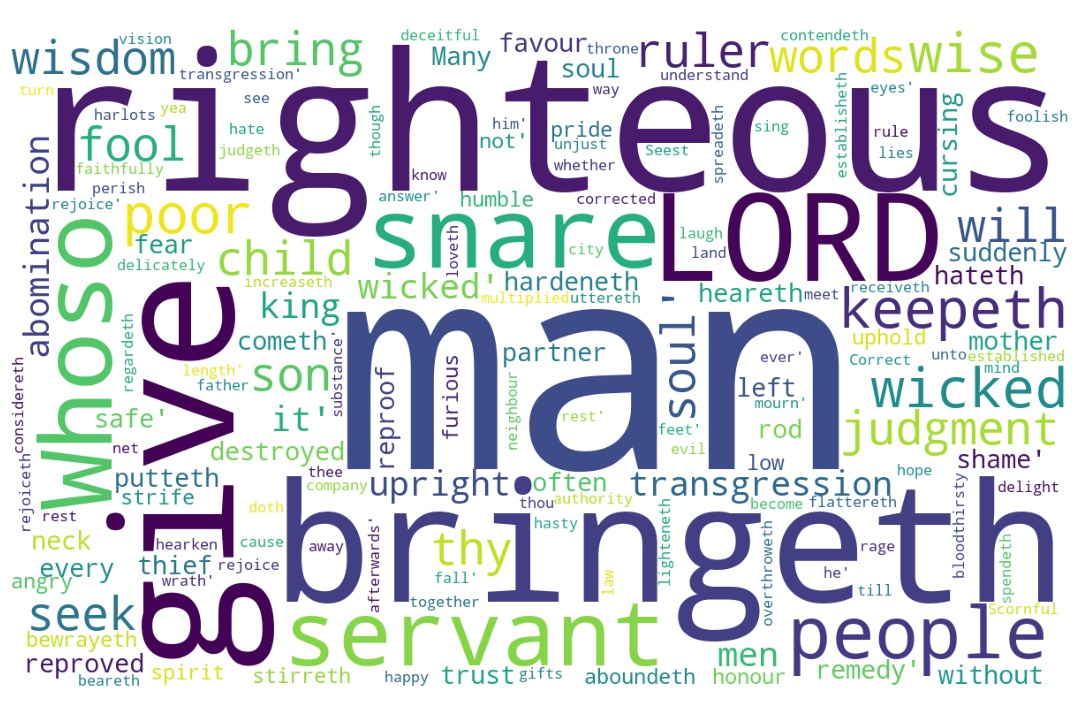
\includegraphics[width=\linewidth]{20OT-Proverbs/Proverb29-WordCloud.jpg}
  \caption{Proverb 29 Word Cloud}
  \label{fig:Proverb 29 word Cloud}
\end{figure}

\marginpar{\scriptsize \centering \fcolorbox{bone}{lime}{\textbf{MISSING WITHOUT WISDOM}}\\ (Proverb 29:1--27) 
\begin{compactenum}[I.][8]
    \item No \textbf{Remedy} \index[scripture]{Proverbs!Pro 29:01}(Pro 29:1) 
    \item No \textbf{Remorse} \index[scripture]{Proverbs!Pro 29:02}(Pro 29:2) 
    \item No \textbf{Rejoicing} \index[scripture]{Proverbs!Pro 29:06}(Pro 29:6) 
    \item No \textbf{Regard} \index[scripture]{Proverbs!Pro 29:07}(Pro 29:7) 
    \item No \textbf{Rest} \index[scripture]{Proverbs!Pro 29:09}(Pro 29:9) 
    \item No \textbf{Reproof} \index[scripture]{Proverbs!Pro 29:15}(Pro 29:15) 
    \item No \textbf{Restraint} \index[scripture]{Proverbs!Pro 29:16}(Pro 29:16) 
\end{compactenum} }

\footnote{\textcolor[cmyk]{0.99998,1,0,0}{\hyperlink{TOC}{Return to end of Table of Contents.}}}\footnote{\href{https://www.audioverse.org/english/audiobibles/books/ENGKJV/O/Prov/1}{\textcolor[cmyk]{0.99998,1,0,0}{Proverbs Audio}}}\textcolor[cmyk]{0.99998,1,0,0}{He, that being often reproved hardeneth \fcolorbox{bone}{bone}{his} neck, shall suddenly be destroyed, and that without \fcolorbox{bone}{lime}{remedy}.}
[2] \textcolor[cmyk]{0.99998,1,0,0}{When the righteous are in authority, the people rejoice: \fcolorbox{bone}{bone}{but} when the wicked beareth rule, the people \fcolorbox{bone}{lime}{mourn}.}
[3] \textcolor[cmyk]{0.99998,1,0,0}{Whoso loveth wisdom rejoiceth \fcolorbox{bone}{bone}{his} father: \fcolorbox{bone}{bone}{but} he that keepeth company with harlots spendeth \emph{his} substance.}
[4] \textcolor[cmyk]{0.99998,1,0,0}{The king by judgment establisheth the land: \fcolorbox{bone}{bone}{but} he that receiveth gifts overthroweth it.}
[5] \textcolor[cmyk]{0.99998,1,0,0}{A man that flattereth \fcolorbox{bone}{bone}{his} neighbour spreadeth a net for \fcolorbox{bone}{bone}{his} feet.}
[6] \textcolor[cmyk]{0.99998,1,0,0}{In the transgression of an evil man \emph{there} \emph{is} a snare: \fcolorbox{bone}{bone}{but} the righteous doth sing and \fcolorbox{bone}{lime}{rejoice}.}
[7] \textcolor[cmyk]{0.99998,1,0,0}{The righteous considereth the cause of the poor: \emph{but} the wicked \fcolorbox{bone}{lime}{regardeth} not to know \emph{it}.}
[8] \textcolor[cmyk]{0.99998,1,0,0}{Scornful men bring a city into a snare: \fcolorbox{bone}{bone}{but} wise \emph{men} turn away wrath.}
[9] \textcolor[cmyk]{0.99998,1,0,0}{\emph{If} a wise man contendeth with a foolish man, whether he rage or laugh, \emph{there} \emph{is} no \fcolorbox{bone}{lime}{rest}.}
[10] \textcolor[cmyk]{0.99998,1,0,0}{The bloodthirsty hate the upright: \fcolorbox{bone}{bone}{but} the just seek \fcolorbox{bone}{bone}{his} soul.}
[11] \textcolor[cmyk]{0.99998,1,0,0}{A fool uttereth all \fcolorbox{bone}{bone}{his} mind: \fcolorbox{bone}{bone}{but} a wise \emph{man} keepeth it in till afterwards.}
[12] \textcolor[cmyk]{0.99998,1,0,0}{If a ruler hearken to lies, all \fcolorbox{bone}{bone}{his} servants \emph{are} wicked.}
[13] \textcolor[cmyk]{0.99998,1,0,0}{The poor and the deceitful man meet together: the LORD lighteneth both their eyes.}
[14] \textcolor[cmyk]{0.99998,1,0,0}{The king that faithfully judgeth the poor, \fcolorbox{bone}{bone}{his} throne shall be established for ever.}
[15] \textcolor[cmyk]{0.99998,1,0,0}{The rod and \fcolorbox{bone}{lime}{reproof} give wisdom: \fcolorbox{bone}{bone}{but} a child left \emph{to} \emph{himself} bringeth \fcolorbox{bone}{bone}{his} mother to shame.}
[16] \textcolor[cmyk]{0.99998,1,0,0}{When the wicked are multiplied, \fcolorbox{bone}{lime}{\fcolorbox{bone}{MYGOLD}{transgression} increaseth}: \fcolorbox{bone}{bone}{but} the righteous shall see their fall.}
[17] \textcolor[cmyk]{0.99998,1,0,0}{Correct thy son, and he shall give thee rest; yea, he shall give delight unto thy soul.}
[18] \textcolor[cmyk]{0.99998,1,0,0}{Where \emph{there} \emph{is} no vision, the people perish: \fcolorbox{bone}{bone}{but} he that keepeth the law, happy \emph{is} he.}
[19] \textcolor[cmyk]{0.99998,1,0,0}{A servant will not be corrected by words: for though he understand he will not answer.}
[20] \textcolor[cmyk]{0.99998,1,0,0}{Seest thou a man \emph{that} \emph{is} hasty in \fcolorbox{bone}{bone}{his} words? \emph{there} \emph{is} more hope of a fool than of him.}
[21] \textcolor[cmyk]{0.99998,1,0,0}{He that delicately bringeth up \fcolorbox{bone}{bone}{his} servant from a child shall have him become \emph{his} son at the length.}
[22] \textcolor[cmyk]{0.99998,1,0,0}{An angry man stirreth up strife, and a furious man aboundeth in transgression.}
[23] \textcolor[cmyk]{0.99998,1,0,0}{A man's pride shall bring him low: \fcolorbox{bone}{bone}{but} honour shall uphold the humble in spirit.}
[24] \textcolor[cmyk]{0.99998,1,0,0}{Whoso is partner with a thief hateth \fcolorbox{bone}{bone}{his} own soul: he heareth cursing, and bewrayeth \emph{it} not.}
[25] \textcolor[cmyk]{0.99998,1,0,0}{The fear of man bringeth a snare: \fcolorbox{bone}{bone}{but} whoso putteth \fcolorbox{bone}{bone}{his} trust in the LORD shall be safe.}
[26] \textcolor[cmyk]{0.99998,1,0,0}{Many seek the ruler's favour; \fcolorbox{bone}{bone}{but} \emph{every} man's judgment \emph{cometh} from the LORD.}
[27] \textcolor[cmyk]{0.99998,1,0,0}{An unjust man \emph{is} an abomination to the just: and \emph{he} \emph{that} \emph{is} upright in the way \emph{is} abomination to the wicked.}



\index[NWIV]{16!Proverbs!Pro 29:1}\index[AWIP]{He!Proverbs!Pro 29:1}\index[AWIP]{that!Proverbs!Pro 29:1}\index[AWIP]{that!Proverbs!Pro 29:1 (2)}\index[AWIP]{being!Proverbs!Pro 29:1}\index[AWIP]{often!Proverbs!Pro 29:1}\index[AWIP]{reproved!Proverbs!Pro 29:1}\index[AWIP]{hardeneth!Proverbs!Pro 29:1}\index[AWIP]{his!Proverbs!Pro 29:1}\index[AWIP]{neck!Proverbs!Pro 29:1}\index[AWIP]{shall!Proverbs!Pro 29:1}\index[AWIP]{suddenly!Proverbs!Pro 29:1}\index[AWIP]{be!Proverbs!Pro 29:1}\index[AWIP]{destroyed!Proverbs!Pro 29:1}\index[AWIP]{and!Proverbs!Pro 29:1}\index[AWIP]{without!Proverbs!Pro 29:1}\index[AWIP]{remedy!Proverbs!Pro 29:1}

\index[NWIV]{18!Proverbs!Pro 29:2}\index[AWIP]{When!Proverbs!Pro 29:2}\index[AWIP]{the!Proverbs!Pro 29:2}\index[AWIP]{the!Proverbs!Pro 29:2 (2)}\index[AWIP]{the!Proverbs!Pro 29:2 (3)}\index[AWIP]{the!Proverbs!Pro 29:2 (4)}\index[AWIP]{righteous!Proverbs!Pro 29:2}\index[AWIP]{are!Proverbs!Pro 29:2}\index[AWIP]{in!Proverbs!Pro 29:2}\index[AWIP]{authority!Proverbs!Pro 29:2}\index[AWIP]{people!Proverbs!Pro 29:2}\index[AWIP]{people!Proverbs!Pro 29:2 (2)}\index[AWIP]{rejoice!Proverbs!Pro 29:2}\index[AWIP]{but!Proverbs!Pro 29:2}\index[AWIP]{when!Proverbs!Pro 29:2}\index[AWIP]{wicked!Proverbs!Pro 29:2}\index[AWIP]{beareth!Proverbs!Pro 29:2}\index[AWIP]{rule!Proverbs!Pro 29:2}\index[AWIP]{mourn!Proverbs!Pro 29:2}

\index[NWIV]{16!Proverbs!Pro 29:3}\index[AWIP]{Whoso!Proverbs!Pro 29:3}\index[AWIP]{loveth!Proverbs!Pro 29:3}\index[AWIP]{wisdom!Proverbs!Pro 29:3}\index[AWIP]{rejoiceth!Proverbs!Pro 29:3}\index[AWIP]{his!Proverbs!Pro 29:3}\index[AWIP]{father!Proverbs!Pro 29:3}\index[AWIP]{but!Proverbs!Pro 29:3}\index[AWIP]{he!Proverbs!Pro 29:3}\index[AWIP]{that!Proverbs!Pro 29:3}\index[AWIP]{keepeth!Proverbs!Pro 29:3}\index[AWIP]{company!Proverbs!Pro 29:3}\index[AWIP]{with!Proverbs!Pro 29:3}\index[AWIP]{harlots!Proverbs!Pro 29:3}\index[AWIP]{spendeth!Proverbs!Pro 29:3}\index[AWIP]{\emph{his}!Proverbs!Pro 29:3}\index[AWIP]{substance!Proverbs!Pro 29:3}\index[AWIP]{\emph{his}!Proverbs!Pro 29:3}

\index[NWIV]{14!Proverbs!Pro 29:4}\index[AWIP]{The!Proverbs!Pro 29:4}\index[AWIP]{king!Proverbs!Pro 29:4}\index[AWIP]{by!Proverbs!Pro 29:4}\index[AWIP]{judgment!Proverbs!Pro 29:4}\index[AWIP]{establisheth!Proverbs!Pro 29:4}\index[AWIP]{the!Proverbs!Pro 29:4}\index[AWIP]{land!Proverbs!Pro 29:4}\index[AWIP]{but!Proverbs!Pro 29:4}\index[AWIP]{he!Proverbs!Pro 29:4}\index[AWIP]{that!Proverbs!Pro 29:4}\index[AWIP]{receiveth!Proverbs!Pro 29:4}\index[AWIP]{gifts!Proverbs!Pro 29:4}\index[AWIP]{overthroweth!Proverbs!Pro 29:4}\index[AWIP]{it!Proverbs!Pro 29:4}

\index[NWIV]{12!Proverbs!Pro 29:5}\index[AWIP]{A!Proverbs!Pro 29:5}\index[AWIP]{man!Proverbs!Pro 29:5}\index[AWIP]{that!Proverbs!Pro 29:5}\index[AWIP]{flattereth!Proverbs!Pro 29:5}\index[AWIP]{his!Proverbs!Pro 29:5}\index[AWIP]{his!Proverbs!Pro 29:5 (2)}\index[AWIP]{neighbour!Proverbs!Pro 29:5}\index[AWIP]{spreadeth!Proverbs!Pro 29:5}\index[AWIP]{a!Proverbs!Pro 29:5}\index[AWIP]{net!Proverbs!Pro 29:5}\index[AWIP]{for!Proverbs!Pro 29:5}\index[AWIP]{feet!Proverbs!Pro 29:5}

\index[NWIV]{18!Proverbs!Pro 29:6}\index[AWIP]{In!Proverbs!Pro 29:6}\index[AWIP]{the!Proverbs!Pro 29:6}\index[AWIP]{the!Proverbs!Pro 29:6 (2)}\index[AWIP]{transgression!Proverbs!Pro 29:6}\index[AWIP]{of!Proverbs!Pro 29:6}\index[AWIP]{an!Proverbs!Pro 29:6}\index[AWIP]{evil!Proverbs!Pro 29:6}\index[AWIP]{man!Proverbs!Pro 29:6}\index[AWIP]{\emph{there}!Proverbs!Pro 29:6}\index[AWIP]{\emph{is}!Proverbs!Pro 29:6}\index[AWIP]{a!Proverbs!Pro 29:6}\index[AWIP]{snare!Proverbs!Pro 29:6}\index[AWIP]{but!Proverbs!Pro 29:6}\index[AWIP]{righteous!Proverbs!Pro 29:6}\index[AWIP]{doth!Proverbs!Pro 29:6}\index[AWIP]{sing!Proverbs!Pro 29:6}\index[AWIP]{and!Proverbs!Pro 29:6}\index[AWIP]{rejoice!Proverbs!Pro 29:6}\index[AWIP]{\emph{there}!Proverbs!Pro 29:6}\index[AWIP]{\emph{is}!Proverbs!Pro 29:6}

\index[NWIV]{16!Proverbs!Pro 29:7}\index[AWIP]{The!Proverbs!Pro 29:7}\index[AWIP]{righteous!Proverbs!Pro 29:7}\index[AWIP]{considereth!Proverbs!Pro 29:7}\index[AWIP]{the!Proverbs!Pro 29:7}\index[AWIP]{the!Proverbs!Pro 29:7 (2)}\index[AWIP]{the!Proverbs!Pro 29:7 (3)}\index[AWIP]{cause!Proverbs!Pro 29:7}\index[AWIP]{of!Proverbs!Pro 29:7}\index[AWIP]{poor!Proverbs!Pro 29:7}\index[AWIP]{\emph{but}!Proverbs!Pro 29:7}\index[AWIP]{wicked!Proverbs!Pro 29:7}\index[AWIP]{regardeth!Proverbs!Pro 29:7}\index[AWIP]{not!Proverbs!Pro 29:7}\index[AWIP]{to!Proverbs!Pro 29:7}\index[AWIP]{know!Proverbs!Pro 29:7}\index[AWIP]{\emph{it}!Proverbs!Pro 29:7}\index[AWIP]{\emph{but}!Proverbs!Pro 29:7}\index[AWIP]{\emph{it}!Proverbs!Pro 29:7}

\index[NWIV]{14!Proverbs!Pro 29:8}\index[AWIP]{Scornful!Proverbs!Pro 29:8}\index[AWIP]{men!Proverbs!Pro 29:8}\index[AWIP]{bring!Proverbs!Pro 29:8}\index[AWIP]{a!Proverbs!Pro 29:8}\index[AWIP]{a!Proverbs!Pro 29:8 (2)}\index[AWIP]{city!Proverbs!Pro 29:8}\index[AWIP]{into!Proverbs!Pro 29:8}\index[AWIP]{snare!Proverbs!Pro 29:8}\index[AWIP]{but!Proverbs!Pro 29:8}\index[AWIP]{wise!Proverbs!Pro 29:8}\index[AWIP]{\emph{men}!Proverbs!Pro 29:8}\index[AWIP]{turn!Proverbs!Pro 29:8}\index[AWIP]{away!Proverbs!Pro 29:8}\index[AWIP]{wrath!Proverbs!Pro 29:8}\index[AWIP]{\emph{men}!Proverbs!Pro 29:8}

\index[NWIV]{18!Proverbs!Pro 29:9}\index[AWIP]{\emph{If}!Proverbs!Pro 29:9}\index[AWIP]{a!Proverbs!Pro 29:9}\index[AWIP]{a!Proverbs!Pro 29:9 (2)}\index[AWIP]{wise!Proverbs!Pro 29:9}\index[AWIP]{man!Proverbs!Pro 29:9}\index[AWIP]{man!Proverbs!Pro 29:9 (2)}\index[AWIP]{contendeth!Proverbs!Pro 29:9}\index[AWIP]{with!Proverbs!Pro 29:9}\index[AWIP]{foolish!Proverbs!Pro 29:9}\index[AWIP]{whether!Proverbs!Pro 29:9}\index[AWIP]{he!Proverbs!Pro 29:9}\index[AWIP]{rage!Proverbs!Pro 29:9}\index[AWIP]{or!Proverbs!Pro 29:9}\index[AWIP]{laugh!Proverbs!Pro 29:9}\index[AWIP]{\emph{there}!Proverbs!Pro 29:9}\index[AWIP]{\emph{is}!Proverbs!Pro 29:9}\index[AWIP]{no!Proverbs!Pro 29:9}\index[AWIP]{rest!Proverbs!Pro 29:9}\index[AWIP]{\emph{If}!Proverbs!Pro 29:9}\index[AWIP]{\emph{there}!Proverbs!Pro 29:9}\index[AWIP]{\emph{is}!Proverbs!Pro 29:9}

\index[NWIV]{11!Proverbs!Pro 29:10}\index[AWIP]{The!Proverbs!Pro 29:10}\index[AWIP]{bloodthirsty!Proverbs!Pro 29:10}\index[AWIP]{hate!Proverbs!Pro 29:10}\index[AWIP]{the!Proverbs!Pro 29:10}\index[AWIP]{the!Proverbs!Pro 29:10 (2)}\index[AWIP]{upright!Proverbs!Pro 29:10}\index[AWIP]{but!Proverbs!Pro 29:10}\index[AWIP]{just!Proverbs!Pro 29:10}\index[AWIP]{seek!Proverbs!Pro 29:10}\index[AWIP]{his!Proverbs!Pro 29:10}\index[AWIP]{soul!Proverbs!Pro 29:10}

\index[NWIV]{15!Proverbs!Pro 29:11}\index[AWIP]{A!Proverbs!Pro 29:11}\index[AWIP]{fool!Proverbs!Pro 29:11}\index[AWIP]{uttereth!Proverbs!Pro 29:11}\index[AWIP]{all!Proverbs!Pro 29:11}\index[AWIP]{his!Proverbs!Pro 29:11}\index[AWIP]{mind!Proverbs!Pro 29:11}\index[AWIP]{but!Proverbs!Pro 29:11}\index[AWIP]{a!Proverbs!Pro 29:11}\index[AWIP]{wise!Proverbs!Pro 29:11}\index[AWIP]{\emph{man}!Proverbs!Pro 29:11}\index[AWIP]{keepeth!Proverbs!Pro 29:11}\index[AWIP]{it!Proverbs!Pro 29:11}\index[AWIP]{in!Proverbs!Pro 29:11}\index[AWIP]{till!Proverbs!Pro 29:11}\index[AWIP]{afterwards!Proverbs!Pro 29:11}\index[AWIP]{\emph{man}!Proverbs!Pro 29:11}

\index[NWIV]{11!Proverbs!Pro 29:12}\index[AWIP]{If!Proverbs!Pro 29:12}\index[AWIP]{a!Proverbs!Pro 29:12}\index[AWIP]{ruler!Proverbs!Pro 29:12}\index[AWIP]{hearken!Proverbs!Pro 29:12}\index[AWIP]{to!Proverbs!Pro 29:12}\index[AWIP]{lies!Proverbs!Pro 29:12}\index[AWIP]{all!Proverbs!Pro 29:12}\index[AWIP]{his!Proverbs!Pro 29:12}\index[AWIP]{servants!Proverbs!Pro 29:12}\index[AWIP]{\emph{are}!Proverbs!Pro 29:12}\index[AWIP]{wicked!Proverbs!Pro 29:12}\index[AWIP]{\emph{are}!Proverbs!Pro 29:12}

\index[NWIV]{14!Proverbs!Pro 29:13}\index[AWIP]{The!Proverbs!Pro 29:13}\index[AWIP]{poor!Proverbs!Pro 29:13}\index[AWIP]{and!Proverbs!Pro 29:13}\index[AWIP]{the!Proverbs!Pro 29:13}\index[AWIP]{the!Proverbs!Pro 29:13 (2)}\index[AWIP]{deceitful!Proverbs!Pro 29:13}\index[AWIP]{man!Proverbs!Pro 29:13}\index[AWIP]{meet!Proverbs!Pro 29:13}\index[AWIP]{together!Proverbs!Pro 29:13}\index[AWIP]{LORD!Proverbs!Pro 29:13}\index[AWIP]{lighteneth!Proverbs!Pro 29:13}\index[AWIP]{both!Proverbs!Pro 29:13}\index[AWIP]{their!Proverbs!Pro 29:13}\index[AWIP]{eyes!Proverbs!Pro 29:13}

\index[NWIV]{14!Proverbs!Pro 29:14}\index[AWIP]{The!Proverbs!Pro 29:14}\index[AWIP]{king!Proverbs!Pro 29:14}\index[AWIP]{that!Proverbs!Pro 29:14}\index[AWIP]{faithfully!Proverbs!Pro 29:14}\index[AWIP]{judgeth!Proverbs!Pro 29:14}\index[AWIP]{the!Proverbs!Pro 29:14}\index[AWIP]{poor!Proverbs!Pro 29:14}\index[AWIP]{his!Proverbs!Pro 29:14}\index[AWIP]{throne!Proverbs!Pro 29:14}\index[AWIP]{shall!Proverbs!Pro 29:14}\index[AWIP]{be!Proverbs!Pro 29:14}\index[AWIP]{established!Proverbs!Pro 29:14}\index[AWIP]{for!Proverbs!Pro 29:14}\index[AWIP]{ever!Proverbs!Pro 29:14}

\index[NWIV]{17!Proverbs!Pro 29:15}\index[AWIP]{The!Proverbs!Pro 29:15}\index[AWIP]{rod!Proverbs!Pro 29:15}\index[AWIP]{and!Proverbs!Pro 29:15}\index[AWIP]{reproof!Proverbs!Pro 29:15}\index[AWIP]{give!Proverbs!Pro 29:15}\index[AWIP]{wisdom!Proverbs!Pro 29:15}\index[AWIP]{but!Proverbs!Pro 29:15}\index[AWIP]{a!Proverbs!Pro 29:15}\index[AWIP]{child!Proverbs!Pro 29:15}\index[AWIP]{left!Proverbs!Pro 29:15}\index[AWIP]{\emph{to}!Proverbs!Pro 29:15}\index[AWIP]{\emph{himself}!Proverbs!Pro 29:15}\index[AWIP]{bringeth!Proverbs!Pro 29:15}\index[AWIP]{his!Proverbs!Pro 29:15}\index[AWIP]{mother!Proverbs!Pro 29:15}\index[AWIP]{to!Proverbs!Pro 29:15}\index[AWIP]{shame!Proverbs!Pro 29:15}\index[AWIP]{\emph{to}!Proverbs!Pro 29:15}\index[AWIP]{\emph{himself}!Proverbs!Pro 29:15}

\index[NWIV]{14!Proverbs!Pro 29:16}\index[AWIP]{When!Proverbs!Pro 29:16}\index[AWIP]{the!Proverbs!Pro 29:16}\index[AWIP]{the!Proverbs!Pro 29:16 (2)}\index[AWIP]{wicked!Proverbs!Pro 29:16}\index[AWIP]{are!Proverbs!Pro 29:16}\index[AWIP]{multiplied!Proverbs!Pro 29:16}\index[AWIP]{transgression!Proverbs!Pro 29:16}\index[AWIP]{increaseth!Proverbs!Pro 29:16}\index[AWIP]{but!Proverbs!Pro 29:16}\index[AWIP]{righteous!Proverbs!Pro 29:16}\index[AWIP]{shall!Proverbs!Pro 29:16}\index[AWIP]{see!Proverbs!Pro 29:16}\index[AWIP]{their!Proverbs!Pro 29:16}\index[AWIP]{fall!Proverbs!Pro 29:16}

\index[NWIV]{17!Proverbs!Pro 29:17}\index[AWIP]{Correct!Proverbs!Pro 29:17}\index[AWIP]{thy!Proverbs!Pro 29:17}\index[AWIP]{thy!Proverbs!Pro 29:17 (2)}\index[AWIP]{son!Proverbs!Pro 29:17}\index[AWIP]{and!Proverbs!Pro 29:17}\index[AWIP]{he!Proverbs!Pro 29:17}\index[AWIP]{he!Proverbs!Pro 29:17 (2)}\index[AWIP]{shall!Proverbs!Pro 29:17}\index[AWIP]{shall!Proverbs!Pro 29:17 (2)}\index[AWIP]{give!Proverbs!Pro 29:17}\index[AWIP]{give!Proverbs!Pro 29:17 (2)}\index[AWIP]{thee!Proverbs!Pro 29:17}\index[AWIP]{rest!Proverbs!Pro 29:17}\index[AWIP]{yea!Proverbs!Pro 29:17}\index[AWIP]{delight!Proverbs!Pro 29:17}\index[AWIP]{unto!Proverbs!Pro 29:17}\index[AWIP]{soul!Proverbs!Pro 29:17}

\index[NWIV]{17!Proverbs!Pro 29:18}\index[AWIP]{Where!Proverbs!Pro 29:18}\index[AWIP]{\emph{there}!Proverbs!Pro 29:18}\index[AWIP]{\emph{is}!Proverbs!Pro 29:18}\index[AWIP]{\emph{is}!Proverbs!Pro 29:18 (2)}\index[AWIP]{no!Proverbs!Pro 29:18}\index[AWIP]{vision!Proverbs!Pro 29:18}\index[AWIP]{the!Proverbs!Pro 29:18}\index[AWIP]{the!Proverbs!Pro 29:18 (2)}\index[AWIP]{people!Proverbs!Pro 29:18}\index[AWIP]{perish!Proverbs!Pro 29:18}\index[AWIP]{but!Proverbs!Pro 29:18}\index[AWIP]{he!Proverbs!Pro 29:18}\index[AWIP]{he!Proverbs!Pro 29:18 (2)}\index[AWIP]{that!Proverbs!Pro 29:18}\index[AWIP]{keepeth!Proverbs!Pro 29:18}\index[AWIP]{law!Proverbs!Pro 29:18}\index[AWIP]{happy!Proverbs!Pro 29:18}\index[AWIP]{\emph{there}!Proverbs!Pro 29:18}\index[AWIP]{\emph{is}!Proverbs!Pro 29:18}\index[AWIP]{\emph{is}!Proverbs!Pro 29:18 (2)}

\index[NWIV]{16!Proverbs!Pro 29:19}\index[AWIP]{A!Proverbs!Pro 29:19}\index[AWIP]{servant!Proverbs!Pro 29:19}\index[AWIP]{will!Proverbs!Pro 29:19}\index[AWIP]{will!Proverbs!Pro 29:19 (2)}\index[AWIP]{not!Proverbs!Pro 29:19}\index[AWIP]{not!Proverbs!Pro 29:19 (2)}\index[AWIP]{be!Proverbs!Pro 29:19}\index[AWIP]{corrected!Proverbs!Pro 29:19}\index[AWIP]{by!Proverbs!Pro 29:19}\index[AWIP]{words!Proverbs!Pro 29:19}\index[AWIP]{for!Proverbs!Pro 29:19}\index[AWIP]{though!Proverbs!Pro 29:19}\index[AWIP]{he!Proverbs!Pro 29:19}\index[AWIP]{he!Proverbs!Pro 29:19 (2)}\index[AWIP]{understand!Proverbs!Pro 29:19}\index[AWIP]{answer!Proverbs!Pro 29:19}

\index[NWIV]{20!Proverbs!Pro 29:20}\index[AWIP]{Seest!Proverbs!Pro 29:20}\index[AWIP]{thou!Proverbs!Pro 29:20}\index[AWIP]{a!Proverbs!Pro 29:20}\index[AWIP]{a!Proverbs!Pro 29:20 (2)}\index[AWIP]{man!Proverbs!Pro 29:20}\index[AWIP]{\emph{that}!Proverbs!Pro 29:20}\index[AWIP]{\emph{is}!Proverbs!Pro 29:20}\index[AWIP]{\emph{is}!Proverbs!Pro 29:20 (2)}\index[AWIP]{hasty!Proverbs!Pro 29:20}\index[AWIP]{in!Proverbs!Pro 29:20}\index[AWIP]{his!Proverbs!Pro 29:20}\index[AWIP]{words?!Proverbs!Pro 29:20}\index[AWIP]{\emph{there}!Proverbs!Pro 29:20}\index[AWIP]{more!Proverbs!Pro 29:20}\index[AWIP]{hope!Proverbs!Pro 29:20}\index[AWIP]{of!Proverbs!Pro 29:20}\index[AWIP]{of!Proverbs!Pro 29:20 (2)}\index[AWIP]{fool!Proverbs!Pro 29:20}\index[AWIP]{than!Proverbs!Pro 29:20}\index[AWIP]{him!Proverbs!Pro 29:20}\index[AWIP]{\emph{that}!Proverbs!Pro 29:20}\index[AWIP]{\emph{is}!Proverbs!Pro 29:20}\index[AWIP]{\emph{is}!Proverbs!Pro 29:20 (2)}\index[AWIP]{\emph{there}!Proverbs!Pro 29:20}

\index[NWIV]{19!Proverbs!Pro 29:21}\index[AWIP]{He!Proverbs!Pro 29:21}\index[AWIP]{that!Proverbs!Pro 29:21}\index[AWIP]{delicately!Proverbs!Pro 29:21}\index[AWIP]{bringeth!Proverbs!Pro 29:21}\index[AWIP]{up!Proverbs!Pro 29:21}\index[AWIP]{his!Proverbs!Pro 29:21}\index[AWIP]{servant!Proverbs!Pro 29:21}\index[AWIP]{from!Proverbs!Pro 29:21}\index[AWIP]{a!Proverbs!Pro 29:21}\index[AWIP]{child!Proverbs!Pro 29:21}\index[AWIP]{shall!Proverbs!Pro 29:21}\index[AWIP]{have!Proverbs!Pro 29:21}\index[AWIP]{him!Proverbs!Pro 29:21}\index[AWIP]{become!Proverbs!Pro 29:21}\index[AWIP]{\emph{his}!Proverbs!Pro 29:21}\index[AWIP]{son!Proverbs!Pro 29:21}\index[AWIP]{at!Proverbs!Pro 29:21}\index[AWIP]{the!Proverbs!Pro 29:21}\index[AWIP]{length!Proverbs!Pro 29:21}\index[AWIP]{\emph{his}!Proverbs!Pro 29:21}

\index[NWIV]{13!Proverbs!Pro 29:22}\index[AWIP]{An!Proverbs!Pro 29:22}\index[AWIP]{angry!Proverbs!Pro 29:22}\index[AWIP]{man!Proverbs!Pro 29:22}\index[AWIP]{man!Proverbs!Pro 29:22 (2)}\index[AWIP]{stirreth!Proverbs!Pro 29:22}\index[AWIP]{up!Proverbs!Pro 29:22}\index[AWIP]{strife!Proverbs!Pro 29:22}\index[AWIP]{and!Proverbs!Pro 29:22}\index[AWIP]{a!Proverbs!Pro 29:22}\index[AWIP]{furious!Proverbs!Pro 29:22}\index[AWIP]{aboundeth!Proverbs!Pro 29:22}\index[AWIP]{in!Proverbs!Pro 29:22}\index[AWIP]{transgression!Proverbs!Pro 29:22}

\index[NWIV]{15!Proverbs!Pro 23:23}\index[AWIP]{A!Proverbs!Pro 23:23}\index[AWIP]{man's!Proverbs!Pro 23:23}\index[AWIP]{pride!Proverbs!Pro 23:23}\index[AWIP]{shall!Proverbs!Pro 23:23}\index[AWIP]{shall!Proverbs!Pro 23:23 (2)}\index[AWIP]{bring!Proverbs!Pro 23:23}\index[AWIP]{him!Proverbs!Pro 23:23}\index[AWIP]{low!Proverbs!Pro 23:23}\index[AWIP]{but!Proverbs!Pro 23:23}\index[AWIP]{honour!Proverbs!Pro 23:23}\index[AWIP]{uphold!Proverbs!Pro 23:23}\index[AWIP]{the!Proverbs!Pro 23:23}\index[AWIP]{humble!Proverbs!Pro 23:23}\index[AWIP]{in!Proverbs!Pro 23:23}\index[AWIP]{spirit!Proverbs!Pro 23:23}

\index[NWIV]{17!Proverbs!Pro 29:24}\index[AWIP]{Whoso!Proverbs!Pro 29:24}\index[AWIP]{is!Proverbs!Pro 29:24}\index[AWIP]{partner!Proverbs!Pro 29:24}\index[AWIP]{with!Proverbs!Pro 29:24}\index[AWIP]{a!Proverbs!Pro 29:24}\index[AWIP]{thief!Proverbs!Pro 29:24}\index[AWIP]{hateth!Proverbs!Pro 29:24}\index[AWIP]{his!Proverbs!Pro 29:24}\index[AWIP]{own!Proverbs!Pro 29:24}\index[AWIP]{soul!Proverbs!Pro 29:24}\index[AWIP]{he!Proverbs!Pro 29:24}\index[AWIP]{heareth!Proverbs!Pro 29:24}\index[AWIP]{cursing!Proverbs!Pro 29:24}\index[AWIP]{and!Proverbs!Pro 29:24}\index[AWIP]{bewrayeth!Proverbs!Pro 29:24}\index[AWIP]{\emph{it}!Proverbs!Pro 29:24}\index[AWIP]{not!Proverbs!Pro 29:24}\index[AWIP]{\emph{it}!Proverbs!Pro 29:24}

\index[NWIV]{18!Proverbs!Pro 29:25}\index[AWIP]{The!Proverbs!Pro 29:25}\index[AWIP]{fear!Proverbs!Pro 29:25}\index[AWIP]{of!Proverbs!Pro 29:25}\index[AWIP]{man!Proverbs!Pro 29:25}\index[AWIP]{bringeth!Proverbs!Pro 29:25}\index[AWIP]{a!Proverbs!Pro 29:25}\index[AWIP]{snare!Proverbs!Pro 29:25}\index[AWIP]{but!Proverbs!Pro 29:25}\index[AWIP]{whoso!Proverbs!Pro 29:25}\index[AWIP]{putteth!Proverbs!Pro 29:25}\index[AWIP]{his!Proverbs!Pro 29:25}\index[AWIP]{trust!Proverbs!Pro 29:25}\index[AWIP]{in!Proverbs!Pro 29:25}\index[AWIP]{the!Proverbs!Pro 29:25}\index[AWIP]{LORD!Proverbs!Pro 29:25}\index[AWIP]{shall!Proverbs!Pro 29:25}\index[AWIP]{be!Proverbs!Pro 29:25}\index[AWIP]{safe!Proverbs!Pro 29:25}

\index[NWIV]{13!Proverbs!Pro 29:26}\index[AWIP]{Many!Proverbs!Pro 29:26}\index[AWIP]{seek!Proverbs!Pro 29:26}\index[AWIP]{the!Proverbs!Pro 29:26}\index[AWIP]{the!Proverbs!Pro 29:26 (2)}\index[AWIP]{ruler's!Proverbs!Pro 29:26}\index[AWIP]{favour!Proverbs!Pro 29:26}\index[AWIP]{but!Proverbs!Pro 29:26}\index[AWIP]{\emph{every}!Proverbs!Pro 29:26}\index[AWIP]{man's!Proverbs!Pro 29:26}\index[AWIP]{judgment!Proverbs!Pro 29:26}\index[AWIP]{\emph{cometh}!Proverbs!Pro 29:26}\index[AWIP]{from!Proverbs!Pro 29:26}\index[AWIP]{LORD!Proverbs!Pro 29:26}\index[AWIP]{\emph{every}!Proverbs!Pro 29:26}\index[AWIP]{\emph{cometh}!Proverbs!Pro 29:26}

\index[NWIV]{22!Proverbs!Pro 29:27}\index[AWIP]{An!Proverbs!Pro 29:27}\index[AWIP]{unjust!Proverbs!Pro 29:27}\index[AWIP]{man!Proverbs!Pro 29:27}\index[AWIP]{\emph{is}!Proverbs!Pro 29:27}\index[AWIP]{\emph{is}!Proverbs!Pro 29:27 (2)}\index[AWIP]{\emph{is}!Proverbs!Pro 29:27 (3)}\index[AWIP]{an!Proverbs!Pro 29:27}\index[AWIP]{abomination!Proverbs!Pro 29:27}\index[AWIP]{abomination!Proverbs!Pro 29:27 (2)}\index[AWIP]{to!Proverbs!Pro 29:27}\index[AWIP]{to!Proverbs!Pro 29:27 (2)}\index[AWIP]{the!Proverbs!Pro 29:27}\index[AWIP]{the!Proverbs!Pro 29:27 (2)}\index[AWIP]{the!Proverbs!Pro 29:27 (3)}\index[AWIP]{just!Proverbs!Pro 29:27}\index[AWIP]{and!Proverbs!Pro 29:27}\index[AWIP]{\emph{he}!Proverbs!Pro 29:27}\index[AWIP]{\emph{that}!Proverbs!Pro 29:27}\index[AWIP]{upright!Proverbs!Pro 29:27}\index[AWIP]{in!Proverbs!Pro 29:27}\index[AWIP]{way!Proverbs!Pro 29:27}\index[AWIP]{wicked!Proverbs!Pro 29:27}\index[AWIP]{\emph{is}!Proverbs!Pro 29:27}\index[AWIP]{\emph{is}!Proverbs!Pro 29:27 (2)}\index[AWIP]{\emph{is}!Proverbs!Pro 29:27 (3)}\index[AWIP]{\emph{he}!Proverbs!Pro 29:27}\index[AWIP]{\emph{that}!Proverbs!Pro 29:27}


\section{Proverb 29 Outlines}

\subsection{My Outlines}

\subsubsection{Things Missing without Wisdom}
%Proverbs 29\footnote{29 May 2016, Keith Anthony}
\index[speaker]{Keith Anthony!Proverb 29 (Things Missing without Wisdom)}
\index[series]{Proverbs (Keith Anthony)!Pro 29 (Things Missing without Wisdom)}
\index[date]{2016/05/29!Proverb 29 (Things Missing without Wisdom) (Keith Anthony)}

\begin{compactenum}[I.]
    \item No \textbf{Remedy} \index[scripture]{Proverbs!Pro 29:01}(Pro 29:1) 
    \item No \textbf{Remorse} \index[scripture]{Proverbs!Pro 29:02}(Pro 29:2) 
    \item No \textbf{Rejoicing} \index[scripture]{Proverbs!Pro 29:06}(Pro 29:6) 
    \item No \textbf{Regard} \index[scripture]{Proverbs!Pro 29:07}(Pro 29:7) 
    \item No \textbf{Rest} \index[scripture]{Proverbs!Pro 29:09}(Pro 29:9) 
    \item No \textbf{Restraint} \index[scripture]{Proverbs!Pro 29:11}(Pro 29:1) 
    \item No \textbf{Reproof} \index[scripture]{Proverbs!Pro 29:15}(Pro 29:15) 
\end{compactenum}

\subsection{Outlines from Others}

 \subsubsection{The People Rejoice - The People Mourn}
\index[speaker]{unknown!Proverb 29:2 (The People Rejoice - The People Mourn)}
\index[series]{Proverbs (unknown)!Pro 29:2 (The People Rejoice - The People Mourn)}
\index[date]{unknown!Proverb 29:2 (The People Rejoice - The People Mourn) (unknown)}
\textbf{Introduction:} About the ``Wicked Ruler'':
\begin{compactenum}[I.][8]
	\item The Wicked Ruler and his  \textbf{People} \index[scripture]{Proverbs!Pro 28:15}(Pro 28:15) \footnote{Temple Baptist Church, Salem Va.}
	\item The Wicked Ruler and his  \textbf{Perception} \index[scripture]{Proverbs!Pro 28:16-17} (Pro 28:16-17) 
	\item The Wicked Ruler and his  \textbf{Perversity} \index[scripture]{Proverbs!Pro 28:18} (Pro 28:18) 
	\item The Wicked Ruler and his  \textbf{Priorities} \index[scripture]{Proverbs!Pro 28:19-22}( Pro 28:19-22) 
	\begin{compactenum}[A.][8]
		\item His Goals \index[scripture]{Proverbs!Pro 28:19} (Pro 28:19) 
		\item His  Guilt \index[scripture]{Proverbs!Pro 28:20} (Pro 28:20) 
		\item His Guile \index[scripture]{Proverbs!Pro 28:21} (Pro 28:21) 
	\end{compactenum}
	\item The Wicked Ruler and his  \textbf{Problems} \index[scripture]{Proverbs!Pro 28:23-27} (Pro 28:23-27) 
	\begin{compactenum}[A.][8]
		\item His Critics \index[scripture]{Proverbs!Pro 28:23} (Pro 28:23) 
		\item His Crimes \index[scripture]{Proverbs!Pro 28:24} (Pro 28:24) 
		\item His Conceit \index[scripture]{Proverbs!Pro 28:25-26} (Pro 28:25-27) 
		\item His Curse \index[scripture]{Proverbs!Pro 28:27} (Pro 28:27) 
	\end{compactenum}
	\item The Wicked Ruler and his  \textbf{Power} \index[scripture]{Proverbs!Pro 28:28} (Pro 28:28) 
	\item The Wicked Ruler and his  \textbf{Punishments} \index[scripture]{Proverbs!Pro 29:01} (Pro 29:1) 
\end{compactenum}
\section{Proverb 29 Comments}

\subsection{Numeric Nuggets}
\textbf{13:} The words ``his'' and ``but'' are used 13 times in Proverb 29. There are 13 words in verses 22 and 26. There are 13 unique words in verses 8, 13, 16, 17, and 19. The only 13-letter word used in Proverb 29 is ``transgression.''


\subsection{Proverb 29:1}
Israel's experience with this is described in a variety of places. Nehemiah 9:16, 9:17, and 9:29 recall Israel before the Babylonian deportation.\footnote{\textbf{Nehemiah 9:16-17} - But they and our fathers dealt proudly, and hardened their necks, and hearkened not to thy commandments, [17] And refused to obey, neither were mindful of thy wonders that thou didst among them; but hardened their necks, and in their rebellion appointed a captain to return to their bondage: but thou art a God ready to pardon, gracious and merciful, slow to anger, and of great kindness, and forsookest them not.}\footnote{\textbf{Nehemiah 9:29} - And testifiedst against them, that thou mightest bring them again unto thy law: yet they dealt proudly, and hearkened not unto thy commandments, but sinned against thy judgments, (which if a man do, he shall live in them;) and withdrew the shoulder, and hardened their neck, and would not hear.}
A promise of this is made way back in Deuteronomy 32.


\subsection{Proverb 29:27}


\subsection{Proverb 29 Repeated Phrases}


%%%%%%%%%%
%%%%%%%%%%
\normalsize
 
\begin{center}
\begin{longtable}{|c|c|}
\caption[Proverb 29 Repeated Phrases]{Proverb 29 Repeated Phrases}\label{table:Repeated Phrases Proverb 29} \\
\hline \multicolumn{1}{|c|}{\textbf{Phrase}} & \multicolumn{1}{c|}{\textbf{Frequency}} \\ \hline 
\endfirsthead
 
\multicolumn{2}{c}
{{\bfseries \tablename\ \thetable{} -- continued from previous page}} \\  
\hline \multicolumn{1}{|c|}{\textbf{Phrase}} & \multicolumn{1}{c|}{\textbf{Frequency}} \\ \hline 
\endhead
 
\hline \multicolumn{2}{c}{{ }} \\ \hline
\endfoot 
the wicked & 4\\ \hline 
\emph{there} \emph{is} & 4\\ \hline 
the righteous & 3\\ \hline 
the people & 3\\ \hline 
but he & 3\\ \hline 
but he that & 3\\ \hline 
he that & 3\\ \hline 
a snare & 3\\ \hline 
a snare but & 3\\ \hline 
snare but & 3\\ \hline 
but the & 3\\ \hline 
the LORD & 3\\ \hline 
\end{longtable}
\end{center}



%%%%%%%%%%
%%%%%%%%%%



%\newpage
\section{Proverb 29 Statistics}

%%%%%%%%%%%%%%%%%%%%%%%%%%%
%%%%% Word Statistics
%%%%%%%%%%%%%%%%%%%%%%%%%%

\normalsize
\subsection{Chapter Word Statistics}


%%%%%%%%%%
%%%%%%%%%%
 
\begin{center}
\begin{longtable}{l|c|c|c|c}
\caption[Stats for Proverb 29]{Stats for Proverb 29} \label{table:Stats for Proverb 29} \\ 
\hline \multicolumn{1}{|c|}{\textbf{Verse(s)}} & \multicolumn{1}{|c|}{\textbf{Count}} & \multicolumn{1}{|c|}{\textbf{Unique}} & \multicolumn{1}{|c|}{\textbf{Italics}} & \multicolumn{1}{|c|}{\textbf{Uniq Italic}}  \\ \hline 
\endfirsthead
 
\multicolumn{5}{c}
{{\bfseries \tablename\ \thetable{} -- continued from previous page}} \\  
\hline \multicolumn{1}{|c|}{\textbf{Verse(s)}} & \multicolumn{1}{|c|}{\textbf{Count}} & \multicolumn{1}{|c|}{\textbf{Unique}} & \multicolumn{1}{|c|}{\textbf{Italics}} & \multicolumn{1}{|c|}{\textbf{Uniq Italic}}  \\ \hline 
\endhead
 
\hline \multicolumn{5}{|r|}{{Continued if needed}} \\ \hline
\endfoot 
1 & 16 & 15 & 0 & 0\\ \hline
2 & 18 & 14 & 0 & 0\\ \hline
3 & 16 & 16 & 1 & 1\\ \hline
4 & 14 & 14 & 0 & 0\\ \hline
5 & 12 & 11 & 0 & 0\\ \hline
6 & 18 & 17 & 2 & 2\\ \hline
7 & 16 & 14 & 2 & 2\\ \hline
8 & 14 & 13 & 1 & 1\\ \hline
9 & 18 & 16 & 3 & 3\\ \hline
10 & 11 & 10 & 0 & 0\\ \hline
11 & 15 & 15 & 1 & 1\\ \hline
12 & 11 & 11 & 1 & 1\\ \hline
13 & 14 & 13 & 0 & 0\\ \hline
14 & 14 & 14 & 0 & 0\\ \hline
15 & 17 & 17 & 2 & 2\\ \hline
16 & 14 & 13 & 0 & 0\\ \hline
17 & 17 & 13 & 0 & 0\\ \hline
18 & 17 & 14 & 3 & 2\\ \hline
19 & 16 & 13 & 0 & 0\\ \hline
20 & 20 & 17 & 4 & 3\\ \hline
21 & 19 & 19 & 1 & 1\\ \hline
22 & 13 & 12 & 0 & 0\\ \hline
23 & 15 & 14 & 0 & 0\\ \hline
24 & 17 & 17 & 1 & 1\\ \hline
25 & 18 & 18 & 0 & 0\\ \hline
26 & 13 & 12 & 2 & 2\\ \hline
27 & 22 & 16 & 5 & 3\\ \hline
\hline \hline
Total & 425 & 214 & 29 & 15




\end{longtable}
\end{center}

%%%%%%%%%%
%%%%%%%%%%


\subsection{Words by Frequency}

\begin{center}
\begin{longtable}{l|r}
\caption[Word Frequencies in Proverb 29]{Word Frequencies in Proverb 29} \label{table:WordsIn-Proverb-29} \\ 
\hline \multicolumn{1}{|c|}{\textbf{Word}} & \multicolumn{1}{c|}{\textbf{Frequency}} \\ \hline 
\endfirsthead
  
\multicolumn{2}{c}  
{{\bfseries \tablename\ \thetable{} -- continued from previous page}} \\   
\hline \multicolumn{1}{|c|}{\textbf{Word}} & \multicolumn{1}{c|}{\textbf{Frequency}} \\ \hline   
\endhead  
  
\hline \multicolumn{2}{|r|}{{Continue}} \\ \hline  
\endfoot  
  
\hline \hline  
\endlastfoot  
  
the & 27\\ \hline 
a & 15\\ \hline 
his & 13\\ \hline 
but & 13\\ \hline 
he & 10\\ \hline 
man & 10\\ \hline 
shall & 9\\ \hline 
\emph{is} & 9\\ \hline 
that & 8\\ \hline 
and & 8\\ \hline 
in & 7\\ \hline 
The & 7\\ \hline 
wicked & 5\\ \hline 
of & 5\\ \hline 
to & 5\\ \hline 
be & 4\\ \hline 
righteous & 4\\ \hline 
A & 4\\ \hline 
\emph{there} & 4\\ \hline 
not & 4\\ \hline 
people & 3\\ \hline 
keepeth & 3\\ \hline 
with & 3\\ \hline 
for & 3\\ \hline 
transgression & 3\\ \hline 
snare & 3\\ \hline 
poor & 3\\ \hline 
wise & 3\\ \hline 
soul & 3\\ \hline 
LORD & 3\\ \hline 
give & 3\\ \hline 
bringeth & 3\\ \hline 
him & 3\\ \hline 
He & 2\\ \hline 
When & 2\\ \hline 
are & 2\\ \hline 
rejoice & 2\\ \hline 
Whoso & 2\\ \hline 
wisdom & 2\\ \hline 
\emph{his} & 2\\ \hline 
king & 2\\ \hline 
by & 2\\ \hline 
judgment & 2\\ \hline 
it & 2\\ \hline 
an & 2\\ \hline 
\emph{it} & 2\\ \hline 
bring & 2\\ \hline 
no & 2\\ \hline 
rest & 2\\ \hline 
upright & 2\\ \hline 
just & 2\\ \hline 
seek & 2\\ \hline 
fool & 2\\ \hline 
all & 2\\ \hline 
their & 2\\ \hline 
child & 2\\ \hline 
thy & 2\\ \hline 
son & 2\\ \hline 
servant & 2\\ \hline 
will & 2\\ \hline 
words & 2\\ \hline 
\emph{that} & 2\\ \hline 
up & 2\\ \hline 
from & 2\\ \hline 
An & 2\\ \hline 
man's & 2\\ \hline 
abomination & 2\\ \hline 
being & 1\\ \hline 
often & 1\\ \hline 
reproved & 1\\ \hline 
hardeneth & 1\\ \hline 
neck & 1\\ \hline 
suddenly & 1\\ \hline 
destroyed & 1\\ \hline 
without & 1\\ \hline 
remedy & 1\\ \hline 
authority & 1\\ \hline 
when & 1\\ \hline 
beareth & 1\\ \hline 
rule & 1\\ \hline 
mourn & 1\\ \hline 
loveth & 1\\ \hline 
rejoiceth & 1\\ \hline 
father & 1\\ \hline 
company & 1\\ \hline 
harlots & 1\\ \hline 
spendeth & 1\\ \hline 
substance & 1\\ \hline 
establisheth & 1\\ \hline 
land & 1\\ \hline 
receiveth & 1\\ \hline 
gifts & 1\\ \hline 
overthroweth & 1\\ \hline 
flattereth & 1\\ \hline 
neighbour & 1\\ \hline 
spreadeth & 1\\ \hline 
net & 1\\ \hline 
feet & 1\\ \hline 
In & 1\\ \hline 
evil & 1\\ \hline 
doth & 1\\ \hline 
sing & 1\\ \hline 
considereth & 1\\ \hline 
cause & 1\\ \hline 
\emph{but} & 1\\ \hline 
regardeth & 1\\ \hline 
know & 1\\ \hline 
Scornful & 1\\ \hline 
men & 1\\ \hline 
city & 1\\ \hline 
into & 1\\ \hline 
\emph{men} & 1\\ \hline 
turn & 1\\ \hline 
away & 1\\ \hline 
wrath & 1\\ \hline 
\emph{If} & 1\\ \hline 
contendeth & 1\\ \hline 
foolish & 1\\ \hline 
whether & 1\\ \hline 
rage & 1\\ \hline 
or & 1\\ \hline 
laugh & 1\\ \hline 
bloodthirsty & 1\\ \hline 
hate & 1\\ \hline 
uttereth & 1\\ \hline 
mind & 1\\ \hline 
\emph{man} & 1\\ \hline 
till & 1\\ \hline 
afterwards & 1\\ \hline 
If & 1\\ \hline 
ruler & 1\\ \hline 
hearken & 1\\ \hline 
lies & 1\\ \hline 
servants & 1\\ \hline 
\emph{are} & 1\\ \hline 
deceitful & 1\\ \hline 
meet & 1\\ \hline 
together & 1\\ \hline 
lighteneth & 1\\ \hline 
both & 1\\ \hline 
eyes & 1\\ \hline 
faithfully & 1\\ \hline 
judgeth & 1\\ \hline 
throne & 1\\ \hline 
established & 1\\ \hline 
ever & 1\\ \hline 
rod & 1\\ \hline 
reproof & 1\\ \hline 
left & 1\\ \hline 
\emph{to} & 1\\ \hline 
\emph{himself} & 1\\ \hline 
mother & 1\\ \hline 
shame & 1\\ \hline 
multiplied & 1\\ \hline 
increaseth & 1\\ \hline 
see & 1\\ \hline 
fall & 1\\ \hline 
Correct & 1\\ \hline 
thee & 1\\ \hline 
yea & 1\\ \hline 
delight & 1\\ \hline 
unto & 1\\ \hline 
Where & 1\\ \hline 
vision & 1\\ \hline 
perish & 1\\ \hline 
law & 1\\ \hline 
happy & 1\\ \hline 
corrected & 1\\ \hline 
though & 1\\ \hline 
understand & 1\\ \hline 
answer & 1\\ \hline 
Seest & 1\\ \hline 
thou & 1\\ \hline 
hasty & 1\\ \hline 
more & 1\\ \hline 
hope & 1\\ \hline 
than & 1\\ \hline 
delicately & 1\\ \hline 
have & 1\\ \hline 
become & 1\\ \hline 
at & 1\\ \hline 
length & 1\\ \hline 
angry & 1\\ \hline 
stirreth & 1\\ \hline 
strife & 1\\ \hline 
furious & 1\\ \hline 
aboundeth & 1\\ \hline 
pride & 1\\ \hline 
low & 1\\ \hline 
honour & 1\\ \hline 
uphold & 1\\ \hline 
humble & 1\\ \hline 
spirit & 1\\ \hline 
is & 1\\ \hline 
partner & 1\\ \hline 
thief & 1\\ \hline 
hateth & 1\\ \hline 
own & 1\\ \hline 
heareth & 1\\ \hline 
cursing & 1\\ \hline 
bewrayeth & 1\\ \hline 
fear & 1\\ \hline 
whoso & 1\\ \hline 
putteth & 1\\ \hline 
trust & 1\\ \hline 
safe & 1\\ \hline 
Many & 1\\ \hline 
ruler's & 1\\ \hline 
favour & 1\\ \hline 
\emph{every} & 1\\ \hline 
\emph{cometh} & 1\\ \hline 
unjust & 1\\ \hline 
\emph{he} & 1\\ \hline 
way & 1\\ \hline 
\end{longtable}  
\end{center}  


  
\normalsize  

  
  


\subsection{Words Alphabetically}

\begin{center}
\begin{longtable}{l|r}
\caption[Word Frequencies in Proverb 29]{Word Frequencies in Proverb 29} \label{table:WordsIn-Proverb-29} \\ 
\hline \multicolumn{1}{|c|}{\textbf{Word}} & \multicolumn{1}{c|}{\textbf{Frequency}} \\ \hline 
\endfirsthead
  
\multicolumn{2}{c}  
{{\bfseries \tablename\ \thetable{} -- continued from previous page}} \\   
\hline \multicolumn{1}{|c|}{\textbf{Word}} & \multicolumn{1}{c|}{\textbf{Frequency}} \\ \hline   
\endhead  
  
\hline \multicolumn{2}{|r|}{{Continue}} \\ \hline  
\endfoot  
  
\hline \hline  
\endlastfoot  
  
A & 4\\ \hline 
An & 2\\ \hline 
Correct & 1\\ \hline 
He & 2\\ \hline 
If & 1\\ \hline 
In & 1\\ \hline 
LORD & 3\\ \hline 
Many & 1\\ \hline 
Scornful & 1\\ \hline 
Seest & 1\\ \hline 
The & 7\\ \hline 
When & 2\\ \hline 
Where & 1\\ \hline 
Whoso & 2\\ \hline 
\emph{If} & 1\\ \hline 
\emph{are} & 1\\ \hline 
\emph{but} & 1\\ \hline 
\emph{cometh} & 1\\ \hline 
\emph{every} & 1\\ \hline 
\emph{he} & 1\\ \hline 
\emph{himself} & 1\\ \hline 
\emph{his} & 2\\ \hline 
\emph{is} & 9\\ \hline 
\emph{it} & 2\\ \hline 
\emph{man} & 1\\ \hline 
\emph{men} & 1\\ \hline 
\emph{that} & 2\\ \hline 
\emph{there} & 4\\ \hline 
\emph{to} & 1\\ \hline 
a & 15\\ \hline 
abomination & 2\\ \hline 
aboundeth & 1\\ \hline 
afterwards & 1\\ \hline 
all & 2\\ \hline 
an & 2\\ \hline 
and & 8\\ \hline 
angry & 1\\ \hline 
answer & 1\\ \hline 
are & 2\\ \hline 
at & 1\\ \hline 
authority & 1\\ \hline 
away & 1\\ \hline 
be & 4\\ \hline 
beareth & 1\\ \hline 
become & 1\\ \hline 
being & 1\\ \hline 
bewrayeth & 1\\ \hline 
bloodthirsty & 1\\ \hline 
both & 1\\ \hline 
bring & 2\\ \hline 
bringeth & 3\\ \hline 
but & 13\\ \hline 
by & 2\\ \hline 
cause & 1\\ \hline 
child & 2\\ \hline 
city & 1\\ \hline 
company & 1\\ \hline 
considereth & 1\\ \hline 
contendeth & 1\\ \hline 
corrected & 1\\ \hline 
cursing & 1\\ \hline 
deceitful & 1\\ \hline 
delicately & 1\\ \hline 
delight & 1\\ \hline 
destroyed & 1\\ \hline 
doth & 1\\ \hline 
established & 1\\ \hline 
establisheth & 1\\ \hline 
ever & 1\\ \hline 
evil & 1\\ \hline 
eyes & 1\\ \hline 
faithfully & 1\\ \hline 
fall & 1\\ \hline 
father & 1\\ \hline 
favour & 1\\ \hline 
fear & 1\\ \hline 
feet & 1\\ \hline 
flattereth & 1\\ \hline 
fool & 2\\ \hline 
foolish & 1\\ \hline 
for & 3\\ \hline 
from & 2\\ \hline 
furious & 1\\ \hline 
gifts & 1\\ \hline 
give & 3\\ \hline 
happy & 1\\ \hline 
hardeneth & 1\\ \hline 
harlots & 1\\ \hline 
hasty & 1\\ \hline 
hate & 1\\ \hline 
hateth & 1\\ \hline 
have & 1\\ \hline 
he & 10\\ \hline 
heareth & 1\\ \hline 
hearken & 1\\ \hline 
him & 3\\ \hline 
his & 13\\ \hline 
honour & 1\\ \hline 
hope & 1\\ \hline 
humble & 1\\ \hline 
in & 7\\ \hline 
increaseth & 1\\ \hline 
into & 1\\ \hline 
is & 1\\ \hline 
it & 2\\ \hline 
judgeth & 1\\ \hline 
judgment & 2\\ \hline 
just & 2\\ \hline 
keepeth & 3\\ \hline 
king & 2\\ \hline 
know & 1\\ \hline 
land & 1\\ \hline 
laugh & 1\\ \hline 
law & 1\\ \hline 
left & 1\\ \hline 
length & 1\\ \hline 
lies & 1\\ \hline 
lighteneth & 1\\ \hline 
loveth & 1\\ \hline 
low & 1\\ \hline 
man & 10\\ \hline 
man's & 2\\ \hline 
meet & 1\\ \hline 
men & 1\\ \hline 
mind & 1\\ \hline 
more & 1\\ \hline 
mother & 1\\ \hline 
mourn & 1\\ \hline 
multiplied & 1\\ \hline 
neck & 1\\ \hline 
neighbour & 1\\ \hline 
net & 1\\ \hline 
no & 2\\ \hline 
not & 4\\ \hline 
of & 5\\ \hline 
often & 1\\ \hline 
or & 1\\ \hline 
overthroweth & 1\\ \hline 
own & 1\\ \hline 
partner & 1\\ \hline 
people & 3\\ \hline 
perish & 1\\ \hline 
poor & 3\\ \hline 
pride & 1\\ \hline 
putteth & 1\\ \hline 
rage & 1\\ \hline 
receiveth & 1\\ \hline 
regardeth & 1\\ \hline 
rejoice & 2\\ \hline 
rejoiceth & 1\\ \hline 
remedy & 1\\ \hline 
reproof & 1\\ \hline 
reproved & 1\\ \hline 
rest & 2\\ \hline 
righteous & 4\\ \hline 
rod & 1\\ \hline 
rule & 1\\ \hline 
ruler & 1\\ \hline 
ruler's & 1\\ \hline 
safe & 1\\ \hline 
see & 1\\ \hline 
seek & 2\\ \hline 
servant & 2\\ \hline 
servants & 1\\ \hline 
shall & 9\\ \hline 
shame & 1\\ \hline 
sing & 1\\ \hline 
snare & 3\\ \hline 
son & 2\\ \hline 
soul & 3\\ \hline 
spendeth & 1\\ \hline 
spirit & 1\\ \hline 
spreadeth & 1\\ \hline 
stirreth & 1\\ \hline 
strife & 1\\ \hline 
substance & 1\\ \hline 
suddenly & 1\\ \hline 
than & 1\\ \hline 
that & 8\\ \hline 
the & 27\\ \hline 
thee & 1\\ \hline 
their & 2\\ \hline 
thief & 1\\ \hline 
thou & 1\\ \hline 
though & 1\\ \hline 
throne & 1\\ \hline 
thy & 2\\ \hline 
till & 1\\ \hline 
to & 5\\ \hline 
together & 1\\ \hline 
transgression & 3\\ \hline 
trust & 1\\ \hline 
turn & 1\\ \hline 
understand & 1\\ \hline 
unjust & 1\\ \hline 
unto & 1\\ \hline 
up & 2\\ \hline 
uphold & 1\\ \hline 
upright & 2\\ \hline 
uttereth & 1\\ \hline 
vision & 1\\ \hline 
way & 1\\ \hline 
when & 1\\ \hline 
whether & 1\\ \hline 
whoso & 1\\ \hline 
wicked & 5\\ \hline 
will & 2\\ \hline 
wisdom & 2\\ \hline 
wise & 3\\ \hline 
with & 3\\ \hline 
without & 1\\ \hline 
words & 2\\ \hline 
wrath & 1\\ \hline 
yea & 1\\ \hline 
\end{longtable}  
\end{center}  


  
\normalsize  

  
  
\subsection{Word Lengths in Chapter} 
\normalsize 
\begin{center} 
\begin{longtable}{l|p{3.75in}} 
\caption[Words by Length in Proverb 29]{Words by Length in Proverb 29} \label{table:WordsIn-Proverb-29} \\ 
\hline \multicolumn{1}{|c|}{\textbf{Length}} & \multicolumn{1}{c|}{\textbf{Words}} \\ \hline 
\endfirsthead 
 
\multicolumn{2}{c} 
{{\bfseries \tablename\ \thetable{} -- continued from previous page}} \\ 
\hline \multicolumn{1}{|c|}{\textbf{Length}} & \multicolumn{1}{c|}{\textbf{Words}} \\ \hline 
\endhead 
 
\hline \multicolumn{2}{|r|}{{Continued}} \\ \hline 
\endfoot 
 
\hline \hline 
\endlastfoot 
1 & A, a\\ \hline 
2 & He, be, in, he, by, it, In, of, an, \emph{is}, to, \emph{it}, \emph{If}, or, no, If, \emph{to}, up, at, An, is, \emph{he}\\ \hline 
3 & his, and, the, are, but, \emph{his}, The, man, net, for, \emph{but}, not, men, \emph{men}, all, \emph{man}, \emph{are}, rod, see, thy, son, yea, law, him, low, own, way\\ \hline 
4 & that, neck, When, when, rule, with, king, land, feet, evil, doth, sing, poor, know, city, into, wise, turn, away, rage, rest, hate, just, seek, soul, fool, mind, till, lies, meet, LORD, both, eyes, ever, give, left, fall, thee, unto, will, thou, \emph{that}, more, hope, than, from, have, fear, safe, Many\\ \hline 
5 & being, often, shall, mourn, Whoso, gifts, \emph{there}, snare, cause, bring, wrath, laugh, ruler, their, child, shame, Where, happy, words, Seest, hasty, angry, man's, pride, thief, whoso, trust, \emph{every}\\ \hline 
6 & remedy, people, wicked, loveth, wisdom, father, throne, mother, vision, perish, though, answer, become, length, strife, honour, uphold, humble, spirit, hateth, favour, \emph{cometh}, unjust\\ \hline 
7 & without, rejoice, beareth, keepeth, company, harlots, foolish, whether, upright, hearken, judgeth, reproof, \emph{himself}, Correct, delight, servant, furious, partner, heareth, cursing, putteth, ruler's\\ \hline 
8 & reproved, suddenly, spendeth, judgment, Scornful, uttereth, servants, together, bringeth, stirreth\\ \hline 
9 & hardeneth, destroyed, righteous, authority, rejoiceth, substance, receiveth, neighbour, spreadeth, regardeth, deceitful, corrected, aboundeth, bewrayeth\\ \hline 
10 & flattereth, contendeth, afterwards, lighteneth, faithfully, multiplied, increaseth, understand, delicately\\ \hline 
11 & considereth, established, abomination\\ \hline 
12 & establisheth, overthroweth, bloodthirsty\\ \hline 
13 & transgression\\ \hline 
\end{longtable} 
\end{center} 




%%%%%%%%%%
%%%%%%%%%%
 



%%% For Indexes

%\index[DEVOTIONAL]{TGIF1!Os Hillman (Living for a Cause Greater Than Yourself) - Proverb 19:17!2021/12/21}

%\index[DEVOTIONAL]{TGIF1!Os Hillman (Living for a Cause Greater Than Yourself) - Proverb 19:17!2021/12/21}

















%%% colour: cardinal red - \textcolor[cmyk]{0,0.85,0.70,0.23}{text}


%%%% Example marginpar with a compactenum list --- green color text
%\marginpar{\scriptsize \textcolor[rgb]{0.00,0.545,0.269}{$\rightarrow$7 Abominations: 
%\begin{compactenum}
%	\item A proud look,
%	\item a lying tongue,
%	\item hands that shed innocent blood,
%	\item An heart that deviseth wicked imaginations,
%	\item feet that be swift in running to mischief,
%	\item A false witness that speaketh lies, and
%	\item he that soweth discord among brethren.
%\end{compactenum}}}



%\newpage

%\begin{mdframed}[style=MyFrame]
%\begin{center}
%\begin{longtable}{|p{.5in}|p{3.5in}|}

%\caption[Corruption Alert: Proverbs 18:1]{Corruption Alert: Proverbs 18:1} \label{table:CorruptionProv18:1} \\ 

%\hline  
%\multicolumn{1}{|c|}{\textbf{Version}} & 
%\multicolumn{1}{c|}{\textbf{Corruption}}  \\ \hline 
%\endfirsthead
 
%\multicolumn{2}{c}
%{{\bfseries \tablename\ \thetable{} -- continued from previous page}} \\  \hline  
%\multicolumn{1}{|c|}{\textbf{Version}} & 
%\multicolumn{1}{c|}{\textbf{Corruption}}  \\ \hline 
%\endhead
 
%\hline \multicolumn{2}{|r|}{{Continued on next page}} \\ \hline
%\endfoot 
%\textcolor[rgb]{0.00,0.00,1.00}{AV} & \textcolor[rgb]{0.00,0.00,1.00}{Through desire a man, having separated himself, seeketh \emph{and} intermeddleth with all wisdom.} \\ \hline
%
%ASV &  He that separateth himself seeketh his own desire, And  rageth against all sound wisdom. \\ \hline
%
%CEB &  Unfriendly people look out for themselves; they bicker with sensible people.\\ \hline
%
%ESV & Whoever isolates himself seeks his own desire;  he breaks out against all sound judgment. \\ \hline
%
%NASV &  He who separates himself seeks his own desire, He quarrels against all sound wisdom.\\ \hline
%
%MEV & He who separates himself seeks his own desire; he seeks and quarrels against all wisdom.\\ \hline
%
%NIV &  An unfriendly person pursues selfish ends and against all sound judgment starts quarrels. \\ \hline
%
%NKJV &  A man who isolates himself seeks his own desire; He rages against all wise judgment.\\ \hline
%
%RSV &  He who is estranged seeks pretexts  to break out against all sound judgment.\\ \hline

% \multicolumn{2}{p{4.3in}}{{Modern translations, such as the ASV and others, strike out the first part of the verse, concealing the intent of mankind in genewisdom clearly revealed in scripture. How wonderful is the obfuscated RSV text: ``He who is estranged seeks pretexts.'' What does THAT mean?}} \\ %\hline

%\hline

%\end{longtable}
%\end{center}

%\normalsize 
%\end{mdframed}

%\marginpar{\scriptsize \centering \fcolorbox{black}{lime}{\textbf{OUTIDE THE PLACE OF PROMISE}}\\ (Psalm 137:1--9) 
%\begin{compactenum}[I.][8]
%	\item \textbf{Plight \& Distress} \index[scripture]{Psalms!Psa 137:01} (Psalm 137:1)
%	\item The \textbf{Place Desired} \index[scripture]{Psalms!Psa 137:01} (Psalm 137:1)
%	\item \textbf{Pining \& Despiar} \index[scripture]{Psalms!Psa 137:02} (Psalm 137:2)
%	\item \textbf{Provoked \& Degraded}\index[scripture]{Psalms!Psa 137:03} (Psalm 137:3)
%	\item The \textbf{Predicament Described}\index[scripture]{Psalms!Psa 137:04} (Psalm 137:4)
%	\item A \textbf{Preference Decided}\index[scripture]{Psalms!Psa 137:06} (Psalm 137:6)
%	\item A \textbf{Prediction of Destruction}\index[scripture]{Psalms!Psa 137:08} (Psalm 137:8)
%\end{compactenum} }


%\subsection{Outlines from Others}

%\subsubsection{Words on Wisdom}
%\index[speaker]{John Battles!Proverbs 01 (Words on Wisdom)}
%\index[series]{Proverbs (John Battles)!Proverbs 01 (Words on Wisdom)}
%\index[date]{2016/01/20!Proverbs 01 (Words on Wisdom) (John Battles)}
%\textbf{Lineage}: adpated from S. Conway\\
%\textbf{Introduction}: Proverbs distinctly points out things that a fool does:
%\begin{compactenum}[I.][4]
%	\item \textbf{Welcome to Wisdom} \index[scripture]{Proverbs!Pro 01:01-09}(Proverbs 1:1-9)
%	\item \textbf{Warnings of Wisdom} \index[scripture]{Proverbs!Pro 01:10-19}(Proverbs 1:10-19).
%	\item \textbf{Woe of Wisdom} \index[scripture]{Proverbs!Pro 01:24-32}(Proverbs 1:24-32)
%	\item \textbf{Watchcare of Wisdom} \index[scripture]{Proverbs!Pro 01:33}(Proverbs 1:33).
%\end{compactenum}


%%%%% COLOR FOR MARGINPAR OUTLINES
%% 1  LIME - \marginpar{\scriptsize \centering \fcolorbox{black}{lime}{\textbf{TITLE}}\\ (Passage) 
%% 2. YELLOW - \marginpar{\scriptsize \centering \fcolorbox{black}{yellow}{\textbf{TITLE}}\\ (Passage) 
%% 3. Blue BGND, WHITE LETTERS - \marginpar{\scriptsize \centering \fcolorbox{black}{blue}{\textbf{\textcolor[cmyk]{0,0,0,0}{TITLE}}}\\ (Passage) 
%% 4. black BGND, WHITE LETTERS - \marginpar{\scriptsize \centering \fcolorbox{black}{black}{\textbf{\textcolor[cmyk]{0,0,0,0}{TITLE}}}\\ (Passage) 
%% 5. red BGND, WHITE LETTERS - \marginpar{\scriptsize \centering \fcolorbox{black}{red}{\textbf{\textcolor[cmyk]{0,0,0,0}{TITLE}}}\\ (Passage) 

%%%%%% INCLUSION OF GRAPHIC
%\newpage

%\begin{figure}
%\begin{center}
%\includegraphics[scale=0.5, angle=90]{07OT-Judges/References/b201107i1-large}
%\caption[Summary of the 13 Judges]{Summary of the 13 Judges}
%\label{fig:Summary of the 13 Judges}
%\end{center}
%\end{figure}


%%%%%%%%%%%
%%%%%%%%%%%

% SYTEMATIC THEOLOGY (10 + 2)
% Theology proper – The study of the character of God
% Angelology – The study of angels
% Biblical theology – The study of the Bible
% Christology – The study of Christ
% Ecclesiology – The study of the church
% Eschatology – The study of the end times[5]
% Hamartiology – The study of sin
% Pneumatology – The study of the Holy Spirit
% Soteriology – The study of salvation
% Theological anthropology – The study of the nature of humanity.
% ++
% Moral theology
% Bilical cosomolgy

%%%%%%%%%%%%%%
%%%%%%%%%%%%%%

% \footnote{\href{https://audiobible.com/bible/psalms_91.html}{\textcolor[cmyk]{0.99998,1,0,0}{Psalm 91 Audio}}}

% \marginpar{\scriptsize \centering \fcolorbox{black}{lime}{\textbf{JERUSALEM}}\\
% \fcolorbox{black}{lime}{\textbf{DON'T GO BACK TO EGYPT}} \\ (Isaiah 31:1--9) 

%%%%%%%%%%%%%%
%%% Extra Colors
%%% from https://latexcolor.blogspot.com/2019/10/list-of-latex-colors.html
%%%%%%%%%%%%%%
% \definecolor{champagne}{rgb}{0.97,0.91,0.81}
% \definecolor{bone}{rgb}{0.89,0.85,0.79}
%\titleJE
%

%%%%% EXAMPLE Index entry:
% \index[DOCTRINES]{Eschatology - Millennium!Psalms!Psa 069:036}

%%% for things found 13 times
%\fcolorbox{black}{bone}{TEXT}
\scriptsize

%%%%%%%%%%%%%%%%%%%%%%%%%%%%%
%Indices
%%%%%%%%%%%%%%%%%%%%%%%%%%%%%

\chapter{Indexes}

\printindex[DOCTRINES]
\printindex[scripture]

\printindex[speaker]
%\printindex[series]

\printindex[FACEBOOK]
\printindex[LOCATION]

\printindex[AWIP]


\printbibliography
\end{document}

